\documentclass[a4paper]{article}

\def\nbook {Applied Partial Differential Equations \\ with Fourier Series and Boundary Value Problems}
\def\nbookshort {APDeq}

% Shared preamble. The fallback lets the document build whether the working
% directory is its own folder or the project root.
\IfFileExists{headerapde.tex}{\input{headerapde}}{\input{../headerapde}}

\begin{document}
\maketitle

\newpage
\tableofcontents

\newpage
\section{\textsf{1 - Heat Equation}}

\subsection{\textsf{1.2 - Derivation of the Conduction of Heat in a One-Dimensional Rod}}
% QUESTION 1
\qs{1.2.1}{Briefly explain the minus sign:
\begin{enumerate}[label=(\alph*)]
	\item in conservation law (1.2.3) or (1.2.5) if \( Q = 0 \)
	\item in Fourier's law (1.2.8)
	\item in conservation law (1.2.12), \( \frac{\partial u}{\partial t} = -\frac{\partial \phi}{\partial x} \)
	\item in Fick's law (1.2.13)
\end{enumerate}}

\begin{enumerate}[label=(\alph*)]
	\item Assuming zero internal thermal energy, we have
	\[
		\frac{\partial e}{\partial t} = -\frac{\partial \phi}{\partial x} 
	\]
	The temporal change in thermal energy density is opposite to the spatial change in heat flux. If more heat leaves a unit volume than had entered, the thermal energy density decreases, and vice-versa.
	\item Fourier's law of heat conduction states
	\[
		\phi = -K_{0}\frac{\partial u}{\partial x} 
	\]
	Heat moves in the direction of the negative of the temperature gradient, or from hot to cold regions.
	\item The spatial change in heat flux is opposite to the temporal change in temperature. If more heat leaves a unit volume than had entered, the temperature decreases, and vice-versa.
	\item Fick's law states
	\[
		\phi = -k \frac{\partial u}{\partial x} 
	\]
	The chemical moves in the direction of the negative of the gradient of the chemical concentration, or from more to less concentrated regions.
\end{enumerate}

% QUESTION 2
\qs{1.2.2}{Derive the heat equation for a rod assuming constant thermal properties and no sources.
\begin{enumerate}[label=(\alph*)]
	\item Consider the total thermal energy between \( x \) and \( x + \Delta x \).
	\item Consider the total thermal energy between \( x = a \) and \( x = b \).
\end{enumerate}}

\begin{enumerate}[label=(\alph*)]
	\item For a thin slice of width \( \Delta x \), the rate of change of heat energy is approximately equal to the flow of thermal energy at \( x \) and \( x + \Delta x \).
	\[
		\frac{\partial }{\partial t} \!\left[ e \!\left( x,t \right)A \Delta x \right] \approx \phi \!\left( x, t \right)A - \phi \!\left( x + \Delta x, t \right)A
	\]
	Divide through by \( A \Delta x \) and in the limit as \( \Delta x \rightarrow 0 \), we find
	\[
		\frac{\partial e}{\partial t} = \lim\limits_{\Delta x \to 0} \frac{\phi \!\left( x, t \right) - \phi \!\left( x + \Delta x, t \right)}{\Delta x} = -\frac{\partial \phi}{\partial x}
	\]
	Replacing \( \partial e / \partial t \) with \( c \rho \partial u / \partial t \), where \( c \) is the specific heat and \( \rho \) is the mass density, we have
	\[
		c \rho \frac{\partial u}{\partial t} = -\frac{\partial \phi}{\partial x} 
	\]
	Lastly, we take the spatial derivative of Fourier's law, where \( K_{0} \) is the thermal conductivity
	\[
		\phi = -K_{0}\frac{\partial u}{\partial x} \quad \implies \quad \frac{\partial \phi}{\partial x} = -K_{0}\frac{\partial^{2}u}{\partial x^{2}} 
	\]
	and substitute into the conservation equation to derive the heat equation.
	\[
		\frac{\partial u}{\partial t} = \frac{K_{0}}{c \rho}\frac{\partial^{2}u}{\partial x^{2}} 
	\]
	\item In lieu of the approximation in the previous set-up, consider the integral conservation
	\[
		\frac{d }{d t}\int^{b}_{a} e \!\left( x,t \right) \, dx = \phi \!\left( a,t \right) - \phi \!\left( b,t \right)
	\]
	By the Fundamental Theorem of Calculus and the constancy of \( x \), the left side becomes
	\[
		\int^{b}_{a} \frac{\partial e}{\partial t} \, dx  
	\]
	And the right side
	\[
		-\int^{b}_{a} \frac{\partial \phi}{\partial x} \, dx  
	\]
	Setting equal and combining terms, we find
	\[
		\int^{b}_{a} \!\left[ \frac{\partial e}{\partial t} + \frac{\partial \phi}{\partial x} \right] \, dx = 0
	\]
	from which we can immediately deduce the conservation law. Proceed as in part (a).
\end{enumerate}

\newpage
% QUESTION 3
\qs{1.2.3}{Derive the heat equation for a rod assuming constant thermal properties with variable cross-sectional area \( A \!\left( x \right) \) assuming no sources by considering the total thermal energy between \( x = a \) and \( x = b \).}

By the integral conservation law, we have
\[
	\frac{d }{d t} \int^{b}_{a} e A \!\left( x \right) \, dx = \int^{b}_{a} \frac{\partial e}{\partial t}A \!\left( x \right) \, dx = -\int^{b}_{a} \frac{\partial }{\partial x}\!\left[ \phi \!\left( x,t \right)A \!\left( x \right) \right] \, dx   
\]
From which we can derive
\[
	\frac{\partial e}{\partial t}A \!\left( x \right) + \frac{\partial }{\partial x}\!\left[ \phi \!\left( x,t \right)A \!\left( x \right) \right] = 0 
\]
Replacing \( e \!\left( x,t \right) \) with \( c \rho u \!\left( x,t \right) \) and combining with the Fourier law, conclude
\[
	\frac{\partial u}{\partial t} = \frac{K_{0}}{c \rho A \!\left( x \right)}\frac{\partial }{\partial x}\!\left[ A \!\left( x \right)\frac{\partial u}{\partial x} \right] = \frac{K_{0}}{c \rho} \!\left[ \frac{\partial^{2}u}{\partial x^{2}} + \frac{1}{A \!\left( x \right)}\frac{\partial u}{\partial x}\frac{\partial A}{\partial x} \right]
\]

% QUESTION 4
\qs{1.2.4}{Derive the diffusion equation for a chemical pollutant.
\begin{enumerate}[label=(\alph*)]
	\item Consider the total amount of the chemical in a thin region between \( x \) and \( x + \Delta x \).
	\item Consider the total amount of the chemical between \( x = a \) and \( x = b \).
\end{enumerate}}

\begin{enumerate}[label=(\alph*)]
	\item The derivation is analogous to that of the heat equation for a thin slice, with chemical diffusivity \( k \) in lieu of the thermal diffusivity \( K_{0} / c \rho \).
	\item See 1.2.2(b) with the same comment about the chemical diffusivity as above.
\end{enumerate}

% QUESTION 5
\qs{1.2.5}{Derive an equation for the concentration \( u \!\left( x,t \right) \) of a chemical pollutant if the chemical is produced due to chemical reaction at the rate of \( \alpha u \!\left( \beta - u \right) \) per unit volume.}

One conceptual understanding here is the production of the chemical originates from some \textit{source} \( Q \), which from the conservation law gives us
\[
	\frac{\partial u}{\partial t} + \frac{\partial \phi}{\partial x} = \alpha u \!\left( \beta - u \right)
\]
From Fick's law, substitute \( \phi \) to derive
\[
	\frac{\partial u}{\partial t} - k \frac{\partial^{2}u}{\partial x^{2}} = \alpha u \!\left( \beta - u \right) 
\]
Observe the logistic form on the right. This equation is called the \textbf{Fisher-KPP equation}, named after Ronald Fisher, Andrey Kolmogorov, Ivan Petrovsky, and Nikolai Piskunov.

% QUESTION 6
\qs{1.2.6}{Suppose that the specific heat is a function of position and temperature, \( c \!\left( x,u \right) \).
\begin{enumerate}[label=(\alph*)]
	\item Show that the heat energy per unit mass necessary to raise the temperature of a thin slice of thickness \( \Delta x \) from \( 0^{\circ} \) to \( u \!\left( x,t \right) \) is not \( c \!\left( x \right)u \!\left( x,t \right) \), but instead \( \int^{u}_{0} c \!\left( x,\overline{u} \right) \, d \overline{u} \).
	\item Rederive the heat equation in this case. Show that (1.2.3) remains unchanged.
\end{enumerate}}

\begin{enumerate}[label=(\alph*)]
	\item Since specific heat is, in this instance, a function of temperature and not independent of it, we must integrate with respect to a dummy variable \( \overline{u} \):
	\[
		\int^{u}_{0} c \!\left( x,\overline{u} \right) \, d \overline{u}  
	\]
	Conceptually, the specific heat varies as a function of the temperature for any given \( \!\left( x,t \right) \). For infinitesimal subdivisions of the total change in temperature from \( 0 \) to \( u \), some amount of energy per unit mass \( c \!\left( x,\overline{u} \right) \, d \overline{u} \) is needed. Because this energy per unit mass varies depending on how far we are along the temperature change to \( u \), we integrate to sum those infinitesimal amounts.
	\item The beginning of the derivation proceeds as in the original case: conservation of heat energy mandates that the rate of change of heat energy equals the thermal flux through the boundaries and internal sources.
	\[
		\frac{\partial }{\partial t} \!\left[ e \!\left( x,t \right)A \Delta x \right] \approx \phi \!\left( x,t \right)A - \phi \!\left( x + \Delta x,t \right)A + Q \!\left( x,t \right)A \Delta x
	\]
	which implies equation (1.2.3)
	\[
		\frac{\partial e}{\partial t} + \frac{\partial \phi}{\partial x} = Q 
	\]
	However, what changes is in the calculation of thermal energy density. Instead of the product of specific heat, mass density, and temperature, we have
	\[
		e \!\left( x,t \right) = \rho \!\left( x \right) \int^{u}_{0} c \!\left( x,\overline{u} \right) \, d \overline{u} 
	\]
	Taking the time derivative and applying Leibniz's rule, derive
	\begin{align*}
		\frac{\partial e}{\partial t} & = \rho \!\left( x \right) \frac{\partial }{\partial t}\int^{u}_{0} c \!\left( x,\overline{u} \right) \, d \overline{u} \\
					      & = \rho \!\left( x \right)\!\left[ c \!\left( x,u \right) \frac{\partial u}{\partial t} + \!\left( x \right)\int^{u}_{0} \underbrace{\frac{\partial }{\partial t}c \!\left( x,\overline{u} \right)}_{= 0} \, d \overline{u} \right]
	\end{align*}
	which is analogous to our derivation of the heat equation in the original case. Combine with Fourier's law to get
	\[
		c \!\left( x,u \right) \rho \!\left( x \right) \frac{\partial u}{\partial t} = \frac{\partial }{\partial x} \!\left( K_{0} \frac{\partial u}{\partial x} \right) + Q
	\]
\end{enumerate}

% QUESTION 7
\qs{1.2.7}{Consider conservation of thermal energy (1.2.4) for any segment of a one-dimensional rod \( a \le x \le b \). By using the fundamental theorem of calculus,
\[
	\frac{\partial }{\partial b} \int^{b}_{a} f \!\left( x \right) \, dx = f \!\left( b \right) 
\]
derive the heat equation (1.2.9).}

The formula implies that \( a \) is constant and \( b \) is varying. Take our integral conservation law, and differentiate both sides by \( b \):
\begin{align*}
	\frac{\partial }{\partial b} \int^{b}_{a} \frac{\partial e \!\left( x,t \right)}{\partial t} \, dx & = \frac{\partial }{\partial b} \!\left[ \phi \!\left( a,t \right) - \phi \!\left( b,t \right) + \int^{b}_{a} Q \, dx \right] \\
	   \frac{\partial e \!\left( b,t \right)}{\partial t} & = -\frac{\partial \phi \!\left( b,t \right)}{\partial b} + Q
\end{align*}
which restores the conservation law! From here we can continue as normal to re-derive
\[
	\frac{\partial u}{\partial t} = k \frac{\partial^{2}u}{\partial x^{2}} 
\]
Since \( b \) is the stand-in for our variable, we can revert to the more customary \( x \).

\vspace{12pt}

% QUESTION 8
\qs{1.2.8}{If \( u \!\left( x,t \right) \) is known, give an expression for the total thermal energy contained in a rod \( \!\left( 0 < x < L \right) \).}

For an arbitrary thin slice, the total thermal energy is
\[
	e \!\left( x,t \right) A \Delta x = c \!\left( x \right)u \!\left( x,t \right) \rho \!\left( x \right) A \Delta x 
\]
Integrating for over the length of the rod, we derive
\[
	E \!\left( t \right) = A \int^{L}_{0} c \!\left( x \right) u \!\left( x,t \right) \rho \!\left( x \right) \, dx  
\]

\newpage
% QUESTION 9
\qs{1.2.9}{Consider a thin one-dimensional rod without sources of thermal energy whose lateral surface area is not insulated.
\begin{enumerate}[label=(\alph*)]
	\item Assume that the heat energy flowing out of the lateral sides per unit surface area per unit time is \( w \!\left( x,t \right) \). Derive the partial differential equation for the temperature \( u \!\left( x,t \right) \).
	\item Assume that \( w \!\left( x,t \right) \) is proportional to the temperature difference between the rod \( u \!\left( x,t \right) \) and a known outside temperature \( \gamma \!\left( x,t \right) \). Derive
	\[
		c \rho \frac{\partial u}{\partial t} = \frac{\partial }{\partial x} \!\left( K_{0}\frac{\partial u}{\partial x} \right) - \frac{P}{A}\!\left[ u \!\left( x,t \right) - \gamma \!\left( x,t \right) \right]h \!\left( x \right) 
	\]
	where \( h \!\left( x \right) \) is a positive \( x \)-dependent proportionality, \( P \) is the lateral perimeter, and \( A \) is the cross-sectional area.
	\item Compare (1.2.15) with the equation for a one-dimensional rod whose lateral surfaces are insulated, but with heat sources.
	\item Specialize (1.2.15) to a rod of circular cross section with constant thermal properties and \( 0^{\circ} \) outside temperature.
	\item Consider the assumptions in part (d). Suppose that the temperature in the rod is uniform [i.e., \( u \!\left( x,t \right) = u \!\left( t \right) \)]. Determine \( u \!\left( t \right) \) if initially \( u \!\left( 0 \right) = u_{0} \).
\end{enumerate}}

\begin{enumerate}[label=(\alph*)]
	\item Suppose that \( A \) is the \textit{cross-sectional area} of the rod and \( P \) is its perimeter. Since \( w \!\left( x,t \right) \) is given as energy per unit surface area per unit time, one intuition we can pursue is to sum over all infinitesimal subdivisions of the total \textit{lateral surface area}. \textbf{Note that it is critical that we distinguish between these two separate areas: cross-sectional (over which the heat fluxes \( \pmb{\phi} \) transpire) and lateral (over which heat escapes in the form of \( \pmb{w \!\left( x,t \right)} \))}. Very simply, the lateral surface area is \( P \, dx \) (for a cylinder, \( P \) would be \( 2 \pi r \), and lateral surface area would be that times the length).
	\[
		P \int^{b}_{a} w \!\left( x,t \right) \, dx
	\]
	Observe that this integral is in units of energy per unit time. Taking our integral conservation equation, the temporal change in total energy must then be equal to the difference of the product of the cross-sectional area with the spatial derivative of the fluxes and the outflow of heat energy per unit time.
	\[
		 \frac{d }{d t}\int^{b}_{a} e \!\left( x,t \right)A \, dx = \!\left[ \phi \!\left( a,t \right) - \phi \!\left( b,t \right) \right]A - P \int^{b}_{a} w \!\left( x,t \right) \, dx 
	\]
	Which simplifies to, after dividing through by cross-sectional area \( A \)
	\[
		\int^{b}_{a} \frac{\partial e}{\partial t} \, dx = -\int^{b}_{a} \frac{\partial \phi}{\partial x} \, dx - \frac{P}{A}\int^{b}_{a} w \!\left( x,t \right) \, dx    
	\]
	and from the arbitrariness of the limits, must produce
	\[
		\frac{\partial e}{\partial t} = -\frac{\partial \phi}{\partial x} - \frac{P}{A}w \!\left( x,t \right) 
	\]
	Switching out \( e \!\left( x,t \right) \) for \( c \rho u \!\left( x,t \right) \) and incorporating Fourier's law in place of \( \phi \) gives us
	\[
		c \rho \frac{\partial u}{\partial t} = \frac{\partial }{\partial x}\!\left( K_{0}\frac{\partial u}{\partial x} \right) - \frac{P}{A}w \!\left( x,t \right) 
	\]
	\item Suppose that the proportionality between \( w \!\left( x,t \right) \) and \( u \!\left( x,t \right) - \gamma \!\left( x,t \right) \) varies as a positive function of \( x \). Call that function \( h \!\left( x \right) \). Now we can write
	\[
		 w \!\left( x,t \right) = \!\left[ u \!\left( x,t \right) - \gamma \!\left( x,t \right) \right]h \!\left( x \right)
	\]
	Then substitute the \( w \!\left( x,t \right) \) from the last term of the equation from part (a) with
	\[
		c \rho \frac{\partial u}{\partial t} = \frac{\partial }{\partial x}\!\left( K_{0} \frac{\partial u}{\partial x} \right) - \frac{P}{A}\!\left[ u \!\left( x,t \right) - \gamma \!\left( x,t \right) \right]h \!\left( x \right) 
	\]
	Since \( h \!\left( x \right) \) is positive, we need not worry about dealing with sign alterations on that last term. Physically, suppose that \( u > \gamma \). Then the outside temperature is cooler, so heat transfer is in the opposite direction of the temperature gradient (from the rod to the outside), hence the final term is negative. In the converse direction when \( u < \gamma \), heat flows from the outside to the rod, and the final term is positive. At equality, the final term vanishes, and whether or not the lateral surface area is insulated becomes irrelevant in this special case.
	\item In lieu of non-insulation and in the presence of heat sources, we have
	\[
		c \rho \frac{\partial u}{\partial t} = \frac{\partial }{\partial x}\!\left( K_{0}\frac{\partial u}{\partial x} \right) + Q 
	\]
	One physical takeaway here is whether \( Q \) serves as a \textbf{source} or a \textbf{sink}, in which the sign is positive and negative, respectively. This is analogous to whether heat flows inward or outward, depending on the lateral temperature change. The chief difference is in whether the contribution or subtraction from the temporal change in energy originates from an external lateral temperature gradient or an internal source or sink.
	\item Let \( \gamma = 0 \). Moreover, \( h \!\left( x \right) = h \), \( P = 2 \pi r \), and \( A = \pi r^{2} \) by the assumption of constant thermal properties, where \( r \) is the radius of the rod. We have implicitly taken \( c \), \( \rho \), and \( K_{0} \) to be constants throughout, but let us explicitly assert that they are constants. Then
	\[
		c \rho \frac{\partial u}{\partial t} = K_{0}\frac{\partial^{2}u}{\partial x^{2}} - \frac{2h}{r}u \!\left( x,t \right)
	\]
	Now might be a good time to note the scale invariance of the equation: irrespective of the choice of units (e.g. Kelvin, Celsius, or Fahrenheit) the equation holds.
	\item Assume spatial uniformity in \( u \). This is a truly delightful assumption, for now the second spatial derivative is annihilated, and our partial differential equation reduces to a first-order ordinary differential equation.
	\[
		u' = -\frac{2h}{c \rho r}u 
	\]
	By separable variables, integrate
	\begin{align*}
		\int^{u \!\left( t \right)}_{u_{0}} \frac{dU}{U} & = -\frac{2h}{c \rho r}\int^{t}_{0}  \, dT \\
		\ln\!\left(\frac{u \!\left( t \right)}{u_{0}}\right) & = -\frac{2h}{c \rho r}t \\
		u \!\left( t \right) & = u_{0}e^{-\frac{2h}{c \rho r}t}
	\end{align*}
\end{enumerate}
The solution under this regime of assumptions is that the temperature decreases exponentially with time from the initial temperature of \( u \!\left( 0 \right) = u_{0} \). In the long run as \( t \rightarrow 0 \), \( u \!\left( t \right) \) tends towards 0, and the rod equilibriates with the outside temperature.

\newpage
\subsection{\textsf{1.3 - Boundary Conditions}}
% QUESTION 1
\qs{1.3.1}{Consider a one-dimensional rod, \( 0 \le x \le L \). Assume that the heat energy flowing out of the rod at \( x = L \) is proportional to the temperature difference between the end temperature of the bar and the known external temperature. Derive (1.3.5); briefly, physically explain why \( H > 0 \).}

Recall that our sign convention for \( \phi \!\left( x,t \right) \) is \textbf{positive} for rightward thermal energy flow per time per unit surface area. Let \( u \!\left( L,t \right) \) and \( u_{B} \!\left( t \right) \) be the the temperature of the bar at the right boundary and the external temperature, respectively. Then if \( H \), the heat transfer coefficient, is the proportionality constant, we have
\[
	\phi \!\left( L,t \right) = H \!\left[ u \!\left( L,t \right) - u_{B} \!\left( t \right) \right] 
\]
We need to be clear about the sign convention. Suppose that \( u \!\left( L,t \right) > u_{B} \!\left( t \right) \). Then heat energy will flow from the rod to the external bath. In order to maintain consistency with our sign convention for \( \phi \), this forces \( H > 0 \). Conversely, if \( u \!\left( L,t \right) < u_{B} \!\left( t \right) \), then heat energy propagates from the outside to the rod (right to left), so we require \( \phi < 0 \). Only if \( H > 0 \) does that condition work. Therefore combining with the Fourier heat law, we have equation (1.3.5)
\[
	-K_{0}\!\left( L \right)\frac{\partial u}{\partial x}\!\left( L,t \right) = H \!\left[ u \!\left( L,t \right) - u_{B}\!\left( t \right) \right] 
\]

% QUESTION 2
\qs{1.3.2}{Two one-dimensional rods of different materials joined at \( x = x_{0} \) are said to be in \textbf{perfect thermal contact} if the temperature is continuous at \( x = x_{0} \):
\[
	u \!\left( x_{0}-,t \right) = u \!\left( x_{0}+,t \right) 
\]
and no heat energy is lost at \( x = x_{0} \) (i.e., the heat energy flowing out of one flows into the other). What mathematical equation represents the latter condition at \( x = x_{0} \)? Under what special condition is \( \partial u / \partial x \) continuous at \( x = x_{0} \)?}

Consider two rods labeled \( A \) and \( B \). Since we do not assume they consist of identical materials, we must generalize by assuming two different temperature functions \( u_{A} \), \( u_{B} \) and thermal conductivity constants \( K_{A} \), \( K_{B} \).

\begin{center}
\begin{tikzpicture}[>=Latex, thick]

    % Parameters
    \def\L{8}
    \def\H{2}
    \def\xo{4}

    % Main cylinder body
    \draw (0,0) -- (\L,0);
    \draw (0,\H) -- (\L,\H);

    % Left ellipse
    \draw (0,\H/2) ellipse (0.35 and \H/2);

    % Middle divider
    \draw (\xo,\H/2) ellipse (0.35 and \H/2);

    % Right ellipse
    \draw (\L,\H/2) ellipse (0.35 and \H/2);

    % Labels inside
    \node at (2,\H/2) {\Large $A$};
    \node at (6,\H/2) {\Large $B$};

    % Region labels
    \node at (2,\H+0.25) {$K_A$};
    \node at (6,\H+0.25) {$K_B$};

    % Arrows at interface
    \draw[->] (\xo-0.8,1.2) -- (\xo+0.8,1.2);
    \draw[->] (\xo-0.8,0.8) -- (\xo+0.8,0.8);

    % x-axis labels
    \node[below] at (0,0) {$x=0$};
    \node[below] at (\xo,0) {$x=x_0$};
    \node[below] at (\L,0) {$x=L$};

\end{tikzpicture}
\end{center}

Some physical insights we must draw: firstly, for there to be no loss of heat energy, the \textbf{thermal energy fluxes at the threshold must be equal in magnitude}, for if they were not, heat energy would either accrue or diminish at \( x = x_{0} \), violating the conservation assumption. There is no addition or subtraction of thermal energy from the outside environment. Secondly, the fluxes must be identical in \textbf{direction}, as otherwise we would violate the premise that heat energy propagates from high to cold temperatures. In other words, \textbf{the fluxes across \( \pmb{A} \) and \( \pmb{B} \) are equal} in the limit as \( x_{0}-,x_{0}+ \rightarrow x_{0} \).
\[
	\phi_{A}\!\left( x_{0}-,t \right) = \phi_{B}\!\left( x_{0}+,t \right) 
\]
Using the Fourier heat law and canceling the sign, we have
\[
	K_{A}\!\left( x_{0}- \right)\frac{\partial u_{A}}{\partial x}\!\left( x_{0}-,t \right) = K_{B}\!\left( x_{0}+ \right)\frac{\partial u_{B}}{\partial x}\!\left( x_{0}+,t \right) 
\]
which is our equation for imposing heat conservation at the junction of the rods. To further enforce continuity of the spatial derivative, we must have the partial derivatives equal to each other, which implies that it is only equality of the conductivity constants that leads to continuity of the spatial derivatives.
\[
	K_{A}\!\left( x_{0}- \right) = K_{B}\!\left( x_{0}+ \right) 
\]

% QUESTION 3
\qs{1.3.3}{Consider a bath containing a fluid of specific heat \( c_{f} \) and mass density \( \rho_{f} \) that surrounds the end \( x = L \) of a one-dimensional rod. Suppose that the bath is rapidly-stirred in a manner such that the bath temperature is approximately uniform throughout, equaling the temperature at \( x = L \), \( u \!\left( L,t \right) \). Assume that the bath is thermally insulated except at its perfect thermal contact with the rod, where the bath may be heated or cooled by the rod. Determine an equation for the temperature in the bath. (This will be a boundary condition at the end \( x = L \).) (\textit{Hint}: See Exercise 1.3.2.)}

Before we begin, it helps to illustrate the scenario. Consider a bath with volume \( V_{\text{bath}} \), and let the area of the contact between the rod and the bath be \( A \). The conceptual setup should look something like this:

\begin{center}
\begin{tikzpicture}[>=Latex, thick, scale=0.7]
    % ---- Parameters ----
    \def\bathRx{5}      % bath ellipse x-radius
    \def\bathRy{1.6}    % bath ellipse y-radius
    \def\bathH{3}       % bath height
    \def\rodRx{0.7}     % rod ellipse x-radius
    \def\rodRy{0.22}    % rod ellipse y-radius
    \def\rodTop{5.0}    % y of rod top
    \def\rodBot{-0.2}   % y of rod bottom (x=L face): below the bath rim
    % ---- Bath: side walls, bottom front arc, top ellipse ----
    \draw (-\bathRx,0) -- (-\bathRx,-\bathH);
    \draw (\bathRx,0) -- (\bathRx,-\bathH);
    \draw (-\bathRx,-\bathH) arc[start angle=180, end angle=360, x radius=\bathRx, y radius=\bathRy];
    % ---- Rod: vertical cylinder, end face submerged, centered on bath axis ----
    \draw (-\rodRx,\rodTop) -- (-\rodRx,\rodBot);
    \draw (\rodRx,\rodTop)  -- (\rodRx,\rodBot);
    % rod bottom face (x = L): full ellipse, drawn before bath top so the
    % bath rim overdraws the part of the rod that is inside the fluid
    \draw (0,\rodBot) ellipse[x radius=\rodRx, y radius=\rodRy];
    % ---- Bath top ellipse: drawn AFTER rod so the rim sits in front ----
    \draw (0,0) ellipse[x radius=\bathRx, y radius=\bathRy];
    % redraw the visible (above-rim) portion of the rod walls on top
    \draw (-\rodRx,\rodTop) -- (-\rodRx,0.12);
    \draw (\rodRx,\rodTop)  -- (\rodRx,0.12);
    % rod top (open): front arc dashed to suggest continuation
    \draw[dashed] (-\rodRx,\rodTop) arc[start angle=180, end angle=360, x radius=\rodRx, y radius=\rodRy];
    % ---- Labels and annotations ----
    % flux arrows: emanate from the submerged end face into the fluid
    \draw[->] (-0.28,\rodBot-0.05) -- (-0.28,\rodBot-0.9);
    \draw[->] (0.28,\rodBot-0.05)  -- (0.28,\rodBot-0.9);
    % phi label placed right next to the flux arrows
    \node at (1.2,\rodBot-0.6) {$\phi(L,t)$};
    % x = L label, pointing at the end face
    \node[right] at (\rodRx+0.25,\rodBot) {$x = L$};
    \draw (\rodRx+0.2,\rodBot) -- (\rodRx-0.05,\rodBot);
    % cross-sectional area A, leader curving in from the right
    \node at (3.3,3.7) {Area of Contact $= A$};
    \draw (2.8,3.4) .. controls (2.0,2.4) and (1.2,1.0) .. (0.0,\rodBot+0.02);
    % bath label, placed low and central in clear space
    \node at (0,-\bathH+0.2) {Volume $= V_{\text{bath}}$};
\end{tikzpicture}
\end{center}

With the given quantities, one natural first step might be to calculate the total energy of the bath as 
\[
	e \!\left( L,t \right) = c_{f}\rho_{f}V_{bath}u \!\left( L,t \right)
\]
Notice here \( e \) is defined in the textbook as an energy density, so we will make a slight alteration to that definition by multiplying through by the bath volume to express in terms of energy alone. Moreover, notice that this is an equation purely in terms of time \( t \). Differentiating with respect to time gives us
\[
	\frac{\partial e}{\partial t} = c_{f}\rho_{f}V_{\text{bath}}\frac{\partial u}{\partial t}\!\left( L,t \right) 
\]
From exercise 1.3.2, the physical intuition we are meant to derive is the insight that at the boundary \( x = L \), \textbf{the heat energy fluxes on either infinitesimal flank of the threshold \( \pmb{x = L} \) are equal}. 
\[
	\phi \!\left( L-,t \right) = \phi \!\left( L+,t \right)
\]
Originally, in deriving the heat equation, we considered a sub-section within a single rod, and identified a spatial gradient of the fluxes between the endpoints of that sub-section. In this case, we only have a \textit{singular} point of contact with an external source or sink (the rod), and thus we only have the flux \( \phi \) to concern ourselves with.

Being perspicacious with units, you will observe that \( \partial e / \partial t \) is in units of \( \text{W} \). However, the flux \( \phi \) is in units \( \text{W} / \text{m}^{2} \). One natural intuition to consider is the geometry of the rod is relevant, and particularly the area of the cross-sectional slice of the rod that touches the bath. Then
\[
	\phi \!\left( L,t \right)A = -K_{0} \frac{\partial u \!\left( L,t \right)}{\partial x}A
\]
Specifically, due to energy conservation, the only contribution or subtraction of the total heat energy in the bath will be due to the exchange of heat energy, or the flux, over the perfect thermal contact. Ergo, our final equation is
\[
	\frac{\partial e}{\partial t} = c_{f}\rho_{f}V_{\text{bath}}\frac{\partial u \!\left( L,t \right)}{\partial t} = -K_{0}\frac{\partial u \!\left( L,t \right)}{\partial x}A
\]
Conceptually, suppose the temperature of the bath increases with time. Then the initial temperature of the rod is warmer than that of the bath, and \( \partial u / \partial x < 0 \) corresponds to \( \partial u / \partial t > 0 \). Vice-versa, if \( \partial u / \partial t < 0 \)--temperature of the bath drops over time--then the rod is relatively cooler than the bath, and heat energy moves in the opposite direction.

\newpage
\subsection{\textsf{1.4 - Equilibrium Temperature Distribution}}
% QUESTION 1
\qs{1.4.1}{Determine the equilibrium temperature distribution for a one-dimensional rod with constant thermal properties with the following sources and boundary conditions:
\begin{enumerate}[label=(\alph*)]
	\item \( Q = 0 \), \quad \( u \!\left( 0 \right) = 0 \), \quad \( u \!\left( L \right) = T \)
	\item \( Q = 0 \), \quad \( u \!\left( 0 \right) = T \), \quad \( u \!\left( L \right) = 0 \)
	\item \( Q = 0 \), \quad \( \displaystyle{\frac{\partial u}{\partial x}\!\left( 0 \right) = 0} \), \quad \( u \!\left( L \right) = T \)
	\item \( Q = 0 \), \quad \( u \!\left( 0 \right) = T \), \quad \( \displaystyle{\frac{\partial u}{\partial x}\!\left( L \right) = \alpha} \)
	\item \( \displaystyle{\frac{Q}{K_{0}} = 1} \), \quad \( u \!\left( 0 \right) = T_{1} \), \quad \( u \!\left( L \right) = T_{2} \)
	\item \( \displaystyle{\frac{Q}{K_{0}} = x^{2}} \), \quad \( u \!\left( 0 \right) = T \), \quad \( \displaystyle{\frac{\partial u}{\partial x}\!\left( L \right) = 0} \)
	\item \( Q = 0 \), \quad \( u \!\left( 0 \right) = T \), \quad %
	\( \displaystyle{\frac{\partial u}{\partial x}\!\left( L \right) + u \!\left( L \right) = 0} \)
	\item \( Q = 0 \), \quad \( \displaystyle{\frac{\partial u}{\partial x}\!\left( 0 \right) - \!\left[ u \!\left( 0 \right) - T \right] = 0} \), \quad \( \displaystyle{\frac{\partial u}{\partial x}\!\left( L \right) = \alpha} \)
\end{enumerate}
In these you may assume that \( u \!\left( x,0 \right) = f \!\left( x \right) \).}

\begin{enumerate}[label=(\alph*)]
	\item No source, so we satisfy \( d^{2}u / dx^{2} = 0 \) and derive \( u \!\left( x \right) = C_{1}x + C_{2} \). The boundary conditions imply
	\begin{align*}
		u \!\left( 0 \right) & = C_{2} = 0 \\
		u \!\left( L \right) & = C_{1}L = T
	\end{align*}
	Leading us to equilibrium temperature distribution \( \displaystyle{u \!\left( x \right) = \frac{T}{L}x} \).
	\item Flip the boundary conditions from the previous exercise, and find
	\begin{align*}
		u \!\left( 0 \right) & = C_{2} = T \\
		u \!\left( L \right) & = C_{1}L + C_{2} = 0 \\ 
		      \implies C_{1} & = -\frac{T}{L}
	\end{align*}
	The equilibrium temperature distribution is \( \displaystyle{u \!\left( x \right) = -\frac{T}{L}x + T} \).
	\item We have the same temperature function \( u \!\left( x \right) = C_{1}x + C_{2} \), but this time with a first derivative boundary condition. Derive
	\begin{align*}
		\frac{\partial u}{\partial x}\!\left( 0 \right) & = C_{1} = 0 \\
		u \!\left( L \right) & = C_{2} = T
	\end{align*}
	Leaving us with \( u \!\left( x \right) = T \). Intuitively, this is correct because to have a zero spatial derivative at one end for a linear temperature distribution immediately implies a horizontal function.
	\item Once more, \( u \!\left( x \right) = C_{1}x + C_{2} \). We can intuitively infer that the line will have slope \( \alpha \) and intercept \( T \) at \( x = 0 \). Applying the boundary conditions gives us
	\begin{align*}
		u \!\left( 0 \right) & = C_{2} = T \\
		\frac{\partial u}{\partial x}\!\left( L \right) & = C_{1} = \alpha
	\end{align*}
	Leading us to \( u \!\left( x \right) = \alpha x + T \). Our intuition proved correct for this simple case, but it is a lesson in examining how the nature of internal sources or boundary conditions can influence the shape of the equilibrium temperature distribution.
	\item Now, our source is non-zero. Setting \( \partial u / \partial t = 0 \), we have
	\[
		K_{0}\frac{d^{2}u}{dx^{2}} + K_{0} = 0
	\]
	Divide through by \( K_{0} \) and isolate the second derivative to get
	\[
		\frac{d^{2}u}{dx^{2}} = -1
	\]
	Integrating twice yields the quadratic
	\[
		u \!\left( x \right) = -\frac{x^{2}}{2} + C_{1}x + C_{2} 
	\]
	Imposing the boundary conditions, derive
	\begin{align*}
		u \!\left( 0 \right) & = C_{2} = T_{1} \\
		u \!\left( L \right) & = -\frac{L^{2}}{2} + C_{1}L + T_{1} = T_{2} \\ 
		      \implies C_{1} & = \frac{2 \!\left( T_{2} - T_{1} \right) + L^{2}}{2L}
	\end{align*}
	Leaving us with
	\[
		u \!\left( x \right) = -\frac{x^{2}}{2} + \!\left[ \frac{2 \!\left( T_{2} - T_{1} \right) + L^{2}}{2L} \right]x + T_{1} 
	\]
	\item From
	\[
		K_{0}\frac{d^{2}u}{dx^{2}} + K_{0}x^{2} = 0 
	\]
	Derive
	\[
		u \!\left( x \right) = -\frac{x^{4}}{12} + C_{1}x + C_{2} 
	\]
	And apply boundary conditions
	\begin{align*}
		u \!\left( 0 \right) & = C_{2} = T \\
		\frac{\partial u}{\partial x}\!\left( L \right) & = -\frac{L^{3}}{3} + C_{1} = 0 \\
		\implies C_{1} & = \frac{L^{3}}{3}
	\end{align*}
	Finishing with temperature distribution
	\[
		u \!\left( x \right) = -\frac{x^{4}}{12} + \frac{L^{3}}{3}x + T
	\]
	\item Returning again to the form \( u \!\left( x \right) = C_{1}x + C_{2} \), apply boundary conditions
	\begin{align*}
		u \!\left( 0 \right) & = C_{2} = T \\
		\frac{\partial u}{\partial x}\!\left( L \right) + u \!\left( L \right) & = C_{1}\!\left( 1 + L \right) + T = 0 \\ 
		C_{1} & = -\frac{T}{1 + L}
	\end{align*}
	Leading to
	\[
		u \!\left( x \right) = T \!\left( 1 - \frac{x}{1 + L} \right) 
	\]
	\item Lastly, we finish up this set with, once more, temperature distribution form \( u \!\left( x \right) = C_{1}x + C_{2} \). Applying the boundary conditions gives us coefficients
	\begin{align*}
		\frac{\partial u}{\partial x}\!\left( 0 \right) - \!\left[ u \!\left( 0 \right) - T \right] & = C_{1} - C_{2} + T = 0 \\
		\frac{\partial u}{\partial x}\!\left( L \right) & = C_{1} = \alpha \\ 
		\implies C_{2} & = \alpha + T
	\end{align*}
	and concluding with
	\[
		u \!\left( x \right) = \alpha \!\left( x + 1 \right) + T 
	\]
\end{enumerate}

\newpage
% QUESTION 2
\qs{1.4.2}{Consider the equilibrium temperature distribution for a uniform one-dimensional rod with sources \( Q / K_{0} = x \) of thermal energy, subject to the boundary conditions \( u \!\left( 0 \right) = 0 \) and \( u \!\left( L \right) = 0 \).
\begin{enumerate}[label=(\alph*)]
	\item Determine the heat energy generated per unit time inside the entire rod.
	\item Determine the heat energy flowing out of the rod per unit time at \( x = 0 \) and at \( x = L \).
	\item What relationships should exist between the answers in parts (a) and (b)? 
\end{enumerate}}

\begin{enumerate}[label=(\alph*)]
	\item Conceptually, we have to consider \( Q / K_{0} = x \) as a \textbf{distributed source} of thermal energy, whilst the problem asks about the rate of heat energy generation \textbf{for the entire rod}. Recall that \( Q \) itself is a measure of heat energy per unit volume per unit time. Therefore, the problem entails summing over all of these distributed sources of heat energy internal to the rod, or
	\[
		Q_{\text{total}} = \int^{L}_{0} Q \, dx = K_{0}\int^{L}_{0} x \, dx = \frac{K_{0}L^{2}}{2} 
	\]
	\item The objective here is to calculate the fluxes \( -K_{0} \partial u / \partial x \) at the boundaries. Derive the equilibrium temperature distribution from 
	\[
		K_{0}\frac{d^{2}u}{dx^{2}} + K_{0}x = 0 \quad \implies \quad u \!\left( x \right) = -\frac{x^{3}}{6} + C_{1}x + C_{2} 
	\]
	where applying boundary conditions yields \( u \!\left( 0 \right) = C_{2} = 0 \) and \( u \!\left( L \right) = -L^{3} / 6 + C_{1}L = 0 \), or \( C_{1} = L^{2} / 6 \). Then our function is
	\[
		u \!\left( x \right) = -\frac{x^{3}}{6} + \frac{L^{2}}{6}x 
	\]
	which has spatial derivative
	\[
		\frac{\partial u}{\partial x} = -\frac{x^{2}}{2} + \frac{L^{2}}{6} 
	\]
	The fluxes are then
	\begin{align*}
		\phi \!\left( 0,t \right) & = -K_{0}\frac{\partial u}{\partial x}\!\left( 0,t \right) = -\frac{K_{0}L^{2}}{6} \\
		\phi \!\left( L,t \right) & = -K_{0}\frac{\partial u}{\partial x}\!\left( L,t \right) = K_{0} \frac{L^{2}}{3}
	\end{align*}
	And since \( K_{0} > 0 \), the directionality of the fluxes is clear. Heat energy propagates leftward at \( x = 0 \) and rightward at \( x = L \). Thus at both ends, \textbf{energy leaves the rod}.
	Now, taking a step back, consider the flux component of the heat equation, which gives us the combined heat energy outflow per unit time at \textit{both} boundaries.
	\[
		-\int^{L}_{0} \frac{\partial \phi}{\partial x} \, dx = K_{0}\frac{\partial u}{\partial x}\!\left( L,t \right) - K_{0}\frac{\partial u}{\partial x}\!\left( 0,t \right) = -\frac{K_{0}L^{2}}{2}
	\]
	\item Returning to the key physical premise of the problem: that we are at \textbf{equilibrium state} for temperature, definitionally we know that \( \partial u / \partial t = 0 \). Equivalently, \( \partial e / \partial t = 0 \). \textbf{We can then deduce for the entire bar}
	\[
		\frac{\partial }{\partial t}\int^{L}_{0} e \, dx = -\int^{L}_{0} \frac{\partial \phi}{\partial x} \, dx + Q_{\text{total}} = 0
	\]
	By conservation of heat energy within the rod, the rate of internal heat energy generation must match the rate of outflow at the boundaries. Indeed, we can confirm
	\[
		\frac{\partial }{\partial t}\int^{L}_{0} e \, dx = -\int^{L}_{0} \frac{\partial \phi}{\partial x} \, dx + Q_{\text{total}} = -\frac{K_{0}L^{2}}{2} + \frac{K_{0}L^{2}}{2} = 0
	\]
\end{enumerate}

% QUESTION 3
\qs{1.4.3}{Determine the equilibrium temperature distribution for a one-dimensional rod composed of two different materials in perfect thermal contact at \( x = 1 \). For \( 0 < x < 1 \), there is one material (\( c \rho = 1 \), \( K_{0} = 1 \)) with a constant source (\( Q = 1 \)), whereas for the other \( 1 < x < 2 \), there are no sources (\( Q = 0 \), \( c \rho = 2 \), \( K_{0} = 2 \)) (see Exercise 1.3.2) with \( u \!\left( 0 \right) = 0 \) and \( u \!\left( 2 \right) = 0 \).}

By the assumption of perfect thermal contact, we know that 

\begin{enumerate}[label=(\alph*)]
	\item the temperatures at the boundary must be equal:
	\[
		u_{A}\!\left( 1-,t \right) = u_{B}\!\left( 1+,t \right) 
	\]
	\item the fluxes at the boundary are equal: 
	\[ 
		\phi_{A}\!\left( 1-,t \right) = \phi_{B}\!\left( 1+,t \right) 
	\]
\end{enumerate}

\begin{center}
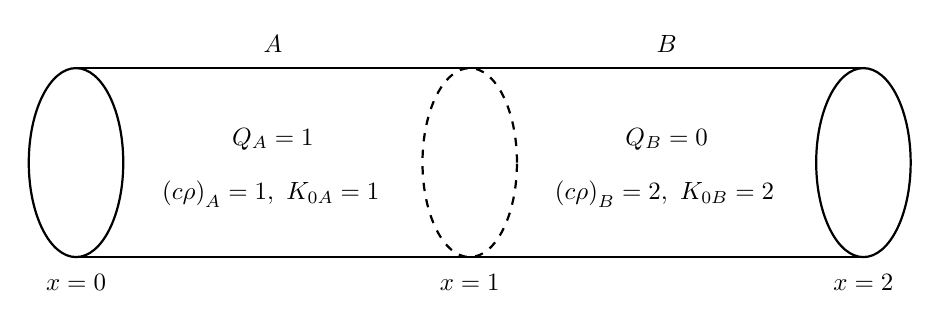
\begin{tikzpicture}[thick, every node/.style={scale=0.9}]

% --- Segment A (x=0 to x=1) ---
\draw (-1,0) ellipse (0.6cm and 1.2cm);
\draw (-1, 1.2) -- (4.0, 1.2);
\draw (-1,-1.2) -- (4.0,-1.2);
\draw[dashed] (4.0, 0) ellipse (0.6cm and 1.2cm);
\node at (1.5, 0.3) {$Q_{A} = 1$};
\node at (1.5, -0.4) {$\!\left( c\rho \right)_{A}=1,\ K_{0A}=1$};
\node at (1.5, 1.5) {$A$};
\node[below] at (-1, -1.3) {$x=0$};
\node[below] at (4.0, -1.3) {$x=1$};

% --- Segment B (x=1 to x=2) ---
\draw (4.0, 1.2) -- (9.0, 1.2);
\draw (4.0,-1.2) -- (9.0,-1.2);
\draw (9.0, 0) ellipse (0.6cm and 1.2cm);
\node at (6.5, 0.3) {$Q_{B} = 0$};
\node at (6.5, -0.4) {$\!\left( c\rho \right)_{B}=2,\ K_{0B}=2$};
\node at (6.5, 1.5) {$B$};
\node[below] at (9.0, -1.3) {$x=2$};

\end{tikzpicture}%
\end{center}

First, let us derive the temperature distributions for sections \( A \) and \( B \) to the extent that we can. In \( A \), we have
\[
	K_{0A}\frac{d^{2}u_{A}}{dx^{2}} + 1 = 0 
\]
Isolating the second derivative and integrating twice, derive
\[
	u_{A}\!\left( x \right) = -\frac{x^{2}}{2} + C_{1A}x + C_{2A}  
\]
Now, from the boundary condition \( u_{A}\!\left( 0 \right) = 0 \), we immediately deduce \( C_{2A} = 0 \), so now we are left with
\[
	u_{A}\!\left( x \right) = -\frac{x^{2}}{2} + C_{1A}x  
\]
Moving onto section \( B \), we have
\[
	\frac{d^{2}u_{B}}{dx^{2}} = 0
\]
which yields
\[
	u_{B}\!\left( x \right) = C_{1B}x + C_{2B}
\]
Imposing the second boundary condition, we can further conclude
\[
	u_{B}\!\left( 2 \right) = 2C_{1B} + C_{2B} = 0 \quad \implies \quad C_{2B} = -2C_{1B}, \quad u_{B}\!\left( x \right) = C_{1B}\!\left( x - 2 \right)
\]
The last component we need is the fluxes, and thus spatial derivatives for both sections, which are
\begin{align*}
	K_{0A}\frac{\partial u_{A}}{\partial x} & = -x + C_{1A} \\
	K_{0B}\frac{\partial u_{B}}{\partial x} & = 2C_{1B}
\end{align*}
Finally, we may apply boundary conditions (a) and (b) at \( x = 1 \).
\begin{alignat*}{5}
	u_{A}\!\left( 1-,t \right) & = -\frac{1}{2} && + C_{1A} && = - && C_{1B} && = u_{B}\!\left( 1+,t \right) \\
	K_{0A}\frac{\partial u_{A}}{\partial x}\!\left( 1-,t \right) & = -1 && + C_{1A} && = && 2C_{1B} && = K_{0B}\frac{\partial u_{B}}{\partial x}\!\left( 1+,t \right)
\end{alignat*}
Solve for this using matrix algebra, using which we find
\[
	C_{1A} = \frac{2}{3}, \quad C_{1B} = -\frac{1}{6}, \quad C_{2B} = \frac{1}{3} 
\]
Giving us equilibrium temperature distribution
\[
	u \!\left( x \right) = \begin{cases}
		\displaystyle{-\frac{x^{2}}{2} + \frac{2}{3}x}, & 0 < x < 1 \\[12pt]
		\displaystyle{-\frac{x}{6} + \frac{1}{3}}, & 1 < x < 2 \\
	\end{cases} 
\]
Observe that \( c \rho \) were irrelevant to this problem, as they matter only in the transient, not equilibrium state.

\vspace{12pt}

% QUESTION 4
\qs{1.4.4}{If both ends of a rod are insulated, derive \textit{from the partial differential equation} that the total thermal energy in the rod is constant.}

By the insulation assumption, we must have
\[
	\frac{\partial u}{\partial x}\!\left( 0,t \right) = \frac{\partial u}{\partial x}\!\left( L,t \right) = 0 
\]
Suppose further that \( u \!\left( x,0 \right) = f \!\left( x \right) \), and \( c \) and \( \rho \) the specific heat and density, respectively. Consider the integral conservation equation
\[
	\frac{d }{d t}\underbrace{\int^{L}_{0} e \, dx}_{\substack{\text{total thermal} \\ \text{energy}}} = \frac{d }{d t}\int^{L}_{0} c \rho u \!\left( x,t \right) \, dx = -\int^{L}_{0} \frac{\partial \phi}{\partial x} \, dx = K_{0}\frac{\partial u}{\partial x}\!\left( L,t \right) - K_{0}\frac{\partial u}{\partial x}\!\left( 0,t \right) = 0
\]
Since the derivative of the total energy density is zero, we may deduce that it is constant.

\vspace{12pt}

% QUESTION 5
\qs{1.4.5}{Consider a one-dimensional rod \( 0 \le x \le L \) of known length and known constant thermal properties without sources. Suppose that the temperature is an \textit{unknown} constant \( T \) at \( x = L \). Determine \( T \) if we know (in the steady state) both the temperature and the heat flow at \( x = 0 \).}

Let \( u \!\left( 0 \right) = T_{1} \) and \( \partial u / \partial x \!\left( 0 \right) \) be known quantities. Since the rod is bereft of internal heat sources, the steady state temperature distribution is of form \( u \!\left( x \right) = C_{1}x + C_{2} \). From the boundary conditions, \( u \!\left( 0 \right) = C_{2} = T_{1} \) and \( \partial u / \partial x \!\left( 0 \right) = C_{1} \). Then \( u \!\left( L \right) \) is
\[
	u \!\left( L \right) = \frac{\partial u}{\partial x}\!\left( 0 \right)L + T_{1}
\]

% QUESTION 6
\qs{1.4.6}{The two ends of a uniform rod of length \( L \) are insulated. There is a constant source of thermal energy \( Q_{0} \neq 0 \), and the temperature is initially \( u \!\left( x,0 \right) = f \!\left( x \right) \).
\begin{enumerate}[label=(\alph*)]
	\item Show mathematically that there does not exist any equilibrium temperature distribution. Briefly explain physically.
	\item Calculate the total thermal energy in the entire rod.
\end{enumerate}}

\begin{enumerate}[label=(\alph*)]
	\item Since insulation implies there is no heat energy flux at the rod's boundaries, the integral conservation equation reduces to
	\[
		\frac{d }{dt}\int^{L}_{0} c \rho u \, dx = \int^{L}_{0} Q_{0} \, dx = Q_{0}L \neq 0
	\]
	which implies that the rate of change of the total thermal energy is never zero. To deduce that we also cannot have \( \partial u / \partial t = 0 \), suppose otherwise. Then \( \partial u / \partial t = 0 \) implies
	\[
		\int^{L}_{0} c \rho \frac{\partial u}{\partial t} \, dx = 0  
	\]
	which immediately contradicts our result. Thus this precludes the existence of an equilibrium temperature distribution.
	\item Integrating from time \( 0 \) to \( t \) and using the dummy variable \( T \), derive
	\begin{align*}		
		\int^{t}_{0} \!\left[ \frac{d }{dT}\int^{L}_{0} c \rho u \!\left( x,T \right) \, dx \right] \, dT & = \int^{t}_{0} \!\left[ \int^{L}_{0} Q_{0} \, dx \right] \, dT \\
		\int^{L}_{0} c \rho u \!\left( x,t \right) \, dx & = \underbrace{\int^{L}_{0} c \rho f \!\left( x \right) \, dx}_{\text{initial thermal energy}} + \underbrace{Q_{0}Lt}_{\text{internal source}}
	\end{align*}
	where we make the substitution \( u \!\left( x,0 \right) = f \!\left( x \right) \). Intuitively, the total thermal energy is a sum of the initial thermal energy and the energy contributed by the heat source over time.
\end{enumerate}

% QUESTION 7
\qs{1.4.7}{For the following problems, determine an equilibrium temperature distribution (if one exists). For what values of \( \beta \) are there solutions? Explain physically.
\begin{enumerate}[label=(\alph*)]
	\item \( \displaystyle{\frac{\partial u}{\partial t} = \frac{\partial^{2}u}{\partial x^{2}} + 1} \), \quad \( u \!\left( x,0 \right) = f \!\left( x \right) \), \quad \( \displaystyle{\frac{\partial u}{\partial x}\!\left( 0,t \right) = 1} \), \quad \( \displaystyle{\frac{\partial u}{\partial x}\!\left( L,t \right) = \beta} \)
	\item \( \displaystyle{\frac{\partial u}{\partial t} = \frac{\partial^{2}u}{\partial x^{2}}} \), \quad \( u \!\left( x,0 \right) = f \!\left( x \right) \), \quad \( \displaystyle{\frac{\partial u}{\partial x}\!\left( 0,t \right) = 1} \), \quad \( \displaystyle{\frac{\partial u}{\partial x}\!\left( L,t \right) = \beta} \)
	\item \( \displaystyle{\frac{\partial u}{\partial t} = \frac{\partial^{2}u}{\partial x^{2}} + x - \beta} \), \quad \( u \!\left( x,0 \right) = f \!\left( x \right) \), \quad \( \displaystyle{\frac{\partial u}{\partial x}\!\left( 0,t \right) = 0} \), \quad \( \displaystyle{\frac{\partial u}{\partial x}\!\left( L,t \right) = 0} \)
\end{enumerate}}

\begin{enumerate}[label=(\alph*)]
	\item Proceed by letting \( \partial u / \partial t = 0 \) to see what becomes of this assumption. We have temperature distribution
	\[
		u \!\left( x \right) = -\frac{x^{2}}{2} + C_{1}x + C_{2} 
	\]
	which has spatial derivative \( \partial u / \partial x = -x + C_{1} \). Then \( \partial u / \partial x \!\left( 0,t \right) = C_{1} = 1 \) and \( \partial u / \partial x \!\left( L,t \right) = 1 - L = \beta \); this is the only permissible value of \( \beta \) for an equilibrium to exist. Unfortunately, we are at a dead end for identifying \( C_{2} \), but this merely sets the vertical position of the equilibrium temperature distribution and can be determined if prescribed temperatures at the ends are given.
	\item Let \( \partial u / \partial t = 0 \). No source, so our temperature distribution is
	\[
		u \!\left( x \right) = C_{1}x + C_{2} 
	\]
	and spatial derivative \( \partial u / \partial x = C_{1} \). Since this is not a function of \( x \) and is constant throughout the rod, the boundary conditions at either end must be equal, so we must have \( C_{1} = \beta = 1 \) for an equilibrium to exist. Again, we have a situation in which \( C_{2} \) cannot be determined, but prescribing temperatures at the boundaries rectifies this.
	\item Let \( \partial u / \partial t = 0 \). Incorporating the distributed heat source, we have temperature distribution
	\[
		u \!\left( x \right) = -\frac{x^{3}}{6} + \frac{\beta x^{2}}{2} + C_{1}x + C_{2} 
	\]
	Then our spatial derivative is 
	\[
		\frac{\partial u}{\partial x} = -\frac{x^{2}}{2} + \beta x + C_{1} 
	\]
	Evaluating at the ends, we get \( \partial u / \partial x \!\left( 0,t \right) = C_{1} = 0 \) and \( \partial u / \partial x \!\left( L,t \right) = \beta L - L^{2} / 2 = 0 \), implying that \( \beta = L / 2 \) for the equilibrium state.
\end{enumerate}

% QUESTION 8
\qs{1.4.8}{Express the integral conservation law for the entire rod with constant thermal properties. Assume the heat flow is known to be different constants at both ends. By integrating with respect to time, determine the total thermal energy in the rod. (Hint: Use the initial condition.)
\begin{enumerate}[label=(\alph*)]
	\item Assume there are no sources.
	\item Assume the sources of thermal energy are constant.
\end{enumerate}}

In both cases, let the initial condition be \( u \!\left( x,0 \right) = f \!\left( x \right) \). Let \( \phi \!\left( 0,t \right) = \alpha \) and \( \phi \!\left( L,t \right) = \beta \).

\begin{enumerate}[label=(\alph*)]
	\item \begin{align*}
			\frac{d }{dt}\int^{L}_{0} c \rho u \, dx & = -\int^{L}_{0} \frac{\partial \phi}{\partial x} \, dx \\
								 & = \phi \!\left( 0,t \right) - \phi \!\left( L,t \right) \\
								 & = \alpha - \beta
	\end{align*}
	Integrate from time \( 0 \) to \( t \) to get
	\begin{alignat*}{2}
		&& \int^{t}_{0} \!\left[ \frac{d }{dT} \int^{L}_{0} c \rho u \!\left( x,T \right) \, dx \right] \, dT & = \int^{t}_{0} \!\left( \alpha - \beta \right) \, dT \\
		\implies && \int^{L}_{0} c \rho u \!\left( x,t \right) \, dx & = \int^{L}_{0} c \rho f \!\left( x \right) \, dx + \!\left( \alpha - \beta \right)t  
	\end{alignat*}
	\item 
	\begin{align*}
		\frac{d }{dt}\int^{L}_{0} c \rho u \, dx & = -\int^{L}_{0} \frac{\partial \phi}{\partial x} \, dx + \int^{L}_{0} Q \, dx \\
							 & = \phi \!\left( 0,t \right) - \phi \!\left( L,t \right) + QL \\
							 & = \alpha - \beta + QL
	\end{align*}
	Integrate from time \( 0 \) to \( t \) to get
	\begin{alignat*}{2}
		&& \int^{t}_{0} \!\left[ \frac{d }{dT}\int^{L}_{0} c \rho u \!\left( x,T \right) \, dx \right] \, dT & = \int^{t}_{0} \!\left( \alpha - \beta + QL \right) \, dT  \\
		\implies && \int^{L}_{0} c \rho u \!\left( x,t \right) \, dx & = \int^{L}_{0} c \rho f \!\left( x \right) \, dx + \!\left( \alpha - \beta + QL \right)t
	\end{alignat*}
\end{enumerate}

% QUESTION 9
\qs{1.4.9}{Derive the integral conservation law for the entire rod with constant thermal properties by integrating the heat equation (1.2.10) (assuming no sources). Show the result is equivalent to (1.2.4).}

The heat equation is
\[
	\frac{\partial u}{\partial t} = k \frac{\partial^{2}u}{\partial x^{2}} 
\]
where \( k = K_{0} / c \rho \). Multiply through by \( c \rho \) and integrate with respect to \( x \) over \( a \le x \le b \) to get
\begin{align*}
	\int^{b}_{a} c \rho \frac{\partial u}{\partial t} \, dx & = K_{0}\int^{b}_{a} \frac{\partial^{2}u}{\partial x^{2}} \, dx \\
								& = K_{0}\!\left[ \frac{\partial u}{\partial x}\!\left( b,t \right) - \frac{\partial u}{\partial x}\!\left( a,t \right) \right] \\
								& = \phi \!\left( a,t \right) - \phi \!\left( b,t \right)
 \end{align*}
By Leibniz's rule, we can pull the differential operator out of the integral. We restore the integral conservation law:
\[
	\frac{d }{dt}\int^{b}_{a} c \rho u \, dx = \phi \!\left( a,t \right) - \phi \!\left( b,t \right)
\]

% QUESTION 10
\qs{1.4.10}{Suppose \( \frac{\partial u}{\partial t} = \frac{\partial^{2}u}{\partial x^{2}} + 4 \), \( u \!\left( x,0 \right) = f \!\left( x \right) \), \( \frac{\partial u}{\partial x}\!\left( 0,t \right) = 5 \), \( \frac{\partial u}{\partial x}\!\left( L,t \right) = 6 \). Calculate the total thermal energy in the one-dimensional rod (as a function of time).}

By the integral conservation law,
\begin{align*}
	\frac{d }{dt}\int^{L}_{0} c \rho u \, dx & = \frac{\partial u}{\partial x}\!\left( L,t \right) - \frac{\partial u}{\partial x}\!\left( 0,t \right) + \int^{L}_{0} 4 \, dx \\
						 & = 6 - 5 + 4L \\
						 & = 1 + 4L
\end{align*}
Integrate from time \( 0 \) to \( t \) to get
\begin{alignat*}{2}
	&& \int^{t}_{0} \!\left[ \frac{d }{dT} \int^{L}_{0} c \rho u \!\left( x,T \right) \, dx \right] \, dT & = \int^{t}_{0} \!\left( 1 + 4L \right) \, dT \\
	\implies && \int^{L}_{0} c \rho u \!\left( x,t \right) \, dx & = \int^{L}_{0} c \rho f \!\left( x \right) \, dx + \!\left( 1 + 4L \right)t \\ 
\end{alignat*}

% QUESTION 11
\qs{1.4.11}{Suppose \( \frac{\partial u}{\partial t} = \frac{\partial^{2}u}{\partial x^{2}} + x \), \( u \!\left( x,0 \right) = f \!\left( x \right) \), \( \frac{\partial u}{\partial x}\!\left( 0,t \right) = \beta \), \( \frac{\partial u}{\partial x}\!\left( L,t \right) = 7 \).
\begin{enumerate}[label=(\alph*)]
	\item Calculate the total thermal energy in the one-dimensional rod (as a function of time).
	\item From part (a), determine the value of \( \beta \) for which an equilibrium exists. For this value of \( \beta \), determine \( \lim\limits_{t \to \infty} u \!\left( x,t \right) \).
\end{enumerate}}

\begin{enumerate}[label=(\alph*)]
	\item By the integral conservation law,
	\begin{align*}
		\frac{d }{dt}\int^{L}_{0} c \rho u \, dx & = \frac{\partial u}{\partial x}\!\left( L,t \right) - \frac{\partial u}{\partial x}\!\left( 0,t \right) + \int^{L}_{0} x \, dx \\
		 & = 7 - \beta + \frac{L^{2}}{2}
	\end{align*}
	Integrating over time from \( 0 \) to \( t \), derive
	\begin{alignat*}{2}
		 && \int^{t}_{0} \!\left[ \frac{d }{dT}\int^{L}_{0} c \rho u \!\left( x,T \right)\, dx \right] \, dT & = \int^{t}_{0} \!\left( 7 - \beta + \frac{L^{2}}{2} \right) \, dT \\
		\implies && \int^{L}_{0} c \rho u \!\left( x,t \right) \, dx & = \int^{L}_{0} c \rho f \!\left( x \right) \, dx + \!\left( 7 - \beta + \frac{L^{2}}{2} \right)t
	\end{alignat*}
	\item Let \( \partial u / \partial t = 0 \). Then
	\[
		u \!\left( x \right) = -\frac{x^{3}}{6} + C_{1}x + C_{2} 
	\]
	with spatial derivative
	\[
		\frac{\partial u}{\partial x} = -\frac{x^{2}}{2} + C_{1} 
	\]
	Applying the boundary conditions, we have
	\begin{align*}
		\frac{\partial u}{\partial x}\!\left( 0,t \right) & = C_{1} = \beta \\
		\frac{\partial u}{\partial x}\!\left( L,t \right) & = \beta - \frac{L^{2}}{2} = 7 \\ 
		\beta & = 7 + \frac{L^{2}}{2}
	\end{align*}
	Then in the steady-state, the temperature distribution is
	\[
		\lim\limits_{t \to \infty} u \!\left( x,t \right) = u \!\left( x \right) = -\frac{x^{3}}{6} + \!\left( 7 + \frac{L^{2}}{2} \right)x + C_{2} 
	\]
	Where \( C_{2} \) is an arbitrary constant dependent on the initial condition.
\end{enumerate}

% QUESTION 12
\qs{1.4.12}{Suppose the concentration \( u \!\left( x,t \right) \) of a chemical satisfies Fick's law (1.2.13), and the initial concentration is given as \( u \!\left( x,0 \right) = f \!\left( x \right) \). Consider a region \( 0 < x < L \) in which the flow is specified at both ends \( -k \frac{\partial u}{\partial x}\!\left( 0,t \right) = \alpha \) and \( -k \frac{\partial u}{\partial x}\!\left( L,t \right) = \beta \). Assume \( \alpha \) and \( \beta \) are constants.
\begin{enumerate}[label=(\alph*)]
	\item Express the conservation law for the entire region.
	\item Determine the total amount of chemical in the region as a function of time (using the initial condition).
	\item Under what conditions is there an equilibrium chemical concentration, and what is it?
\end{enumerate}}

\begin{enumerate}[label=(\alph*)]
	\item \[
		\frac{d }{dt}\int^{L}_{0} u \, dx = -\int^{L}_{0} \frac{\partial \phi}{\partial x} \, dx = -k \!\left[ \frac{\partial u}{\partial x}\!\left( 0,t \right) - \frac{\partial u}{\partial x}\!\left( L,t \right) \right] = \alpha - \beta
	\]
	\item Since we define \( u \!\left( x,t \right) \) as the concentration of the chemical per unit volume, we will need to multiply through by the cross-sectional area of the rod \( A \). Integrate over time from \( 0 \) to \( t \) to get
	\begin{alignat*}{2}
		&& \int^{t}_{0} \!\left[ \frac{d }{dT}\int^{L}_{0} u \!\left( x,T \right)A \, dx  \right] \, dT & = A \int^{t}_{0} \!\left( \alpha - \beta \right) \, dT \\
		\implies && \int^{L}_{0} u \!\left( x,t \right)A \, dx & = A \!\left[ \int^{L}_{0} f \!\left( x \right) \, dx + \!\left( \alpha - \beta \right)t \right]
	\end{alignat*}
	\item Let \( \partial u / \partial t = 0 \). With zero sources, we have chemical concentration
	\[
		u \!\left( x \right) = C_{1}x + C_{2}
	\]
	Applying the boundary conditions, we have
	\[
		\frac{\partial u}{\partial x}\!\left( 0,t \right) = -\frac{\alpha}{k} = C_{1} = -\frac{\beta}{k} = \frac{\partial u}{\partial x}\!\left( L,t \right) 
	\]
	from which we can conclude that equilibrium exists only when \( \alpha = \beta \).
\end{enumerate}

\newpage
% QUESTION 13
\qs{1.4.13}{Do Exercise 1.4.12 if \( \alpha \) and \( \beta \) are functions of time.}

\begin{enumerate}[label=(\alph*)]
	\item Now we assume \( \alpha \) and \( \beta \) are functions of time, which changes the conservation equation to
	\[
		\frac{d }{dt}\int^{L}_{0} u \, dx = -\int^{L}_{0} \frac{\partial \phi}{\partial x} \, dx = -k \!\left[ \frac{\partial u}{\partial x}\!\left( 0,t \right) - \frac{\partial u}{\partial x}\!\left( L,t \right) \right] = \alpha \!\left( t \right) - \beta \!\left( t \right)
	\]
	\item Since \( \alpha \) and \( \beta \) are no longer pure constants, we can only consider their integrals in the abstract as part of the total amount of chemical.
	\[
		\int^{L}_{0} u \!\left( x,t \right)A \, dx = A \!\left[ \int^{L}_{0} f \!\left( x \right) \, dx + \int^{t}_{0} \!\left( \alpha \!\left( T \right) - \beta \!\left( T \right) \right) \, dT \right]  
	\]
	\item Lastly, by assuming \( \partial u / \partial t = 0 \) and that \( \lim\limits_{t \to \infty} u \!\left( x,t \right) = u \!\left( x \right) \), it still follows that \( C_{1} \) is a constant. From the boundary conditions, we still must have
	\[
		-\lim\limits_{t \to \infty}\frac{\alpha \!\left( t \right)}{k} = C_{1} = -\lim\limits_{t \to \infty}\frac{\beta \!\left( t \right)}{k} 
	\]
	In other words, \( \alpha \!\left( t \right) \) and \( \beta \!\left( t \right) \) must approach constants in the temporal limit for a steady-state to exist.
\end{enumerate}

\newpage
\subsection{\textsf{1.5 - Derivation of the Heat Equation in Two or Three Dimensions}}
% QUESTION 1
\qs{1.5.1}{Let \( c \!\left( x,y,z,t \right) \) denote the concentration of a pollutant (the amount per unit volume).
\begin{enumerate}[label=(\alph*)]
	\item What is an expression for the total amount of pollutant in the region \( R \)?
	\item Suppose that the flow \( \pmb{J} \) of the pollutant is proportional to the gradient of the concentration. (Is this reasonable?) Express conservation of the pollutant.
	\item Derive the partial differential equation governing the diffusion of the pollutant.
\end{enumerate}}

\begin{enumerate}[label=(\alph*)]
	\item \( \iiint_{R} c \, dV \)
	\item Let \( \pmb{J} = A \nabla c \). This is simply Fick's law in three dimensions when \( A = -k \).
	\[
		\pmb{J} = -k \nabla c \!\left( x,y,z,t \right) = \frac{\partial c}{\partial x}\pmb{\hat{i}} + \frac{\partial c}{\partial y}\pmb{\hat{j}} + \frac{\partial c}{\partial z}\pmb{\hat{k}}
	\]
	Conservation is when there is no change in mass in the volume, so assuming that the three-dimensional region is invariant with time, we have
	\[
		\frac{d }{dt}\iiint_{R} c \!\left( x,y,z,t \right) \, dV = 0 \quad \implies \quad \frac{\partial c}{\partial t} = 0 
	\]
	\item Conceptually, the rate of change of the amount of pollutant is expressed by
	\[
		\vcenter{\hbox{\shortstack{Rate of change\\of amount\\of pollutant}}}
		\quad=\quad
		\vcenter{\hbox{\shortstack{Surface flux\\of the pollutant\\per unit time}}}
		\quad+\quad
		\vcenter{\hbox{\shortstack{Internal pollutant\\generation\\per unit time}}}
	\]
	It is helpful to visualize the physics with a diagram:
	\begin{center}
	\begin{tikzpicture}[
	  scale=0.7,
	  every node/.style={font=\small},
	  outarrow/.style={-{Stealth[length=6pt]}, line width=1.5pt, color=red!70!black},
	  inarrow/.style={-{Stealth[length=6pt]}, line width=1.5pt, color=blue!70!black},
	  leader/.style={dashed, line width=0.5pt, color=black!40},
	  axis/.style={dashed, line width=0.6pt, color=teal!60!black, opacity=0.5},
	]

	%% ── Sphere ──────────────────────────────────────────────────────────────
	\def\R{5.5cm}
	\coordinate (O) at (0,0);

	\shade[ball color=teal!15, opacity=0.6] (O) circle (\R);
	\draw[teal!60!black, line width=1.5pt] (O) circle (\R);

	\draw[axis] (-\R,0) -- (\R,0);
	\draw[axis] (0,-\R) -- (0,\R);

	%% ── Internal generation sources ────────────────────────────────────────
	\foreach \x/\y/\r in {-1.2/1.1/0.26, 1.1/-0.55/0.26, -0.5/-0.75/0.20, 1.0/1.6/0.18}{
	  \fill[orange!25, opacity=0.4] (\x,\y) circle (\r*1.8 cm);
	  \fill[orange!70, opacity=0.65] (\x,\y) circle (\r cm);
	  \fill[orange!90!brown] (\x,\y) circle (0.07 cm);
	}

	\node[font=\small\itshape, color=orange!60!brown] at (-2.2, 2.2)
	  {$Q$ (generation)};
	\draw[leader] (-1.85,2.05) -- (-1.3,1.2);

	%% ── Surface normal ──────────────────────────────────────────────────────
	\draw[-{Stealth[length=5pt]}, teal!70!black, line width=1pt]
	  (0,\R) -- (0,\R+0.9cm) node[right, font=\footnotesize\itshape]{$\hat{n}$};

	\node[font=\footnotesize, color=teal!50!black] at (3.7, 4.7) {$dS$};
	\draw[leader] (3.05,4.15) -- (2.7,3.7);

	\draw[black!40, dashed, line width=0.7pt] (O) -- (3.4,3.4)
	  node[midway, above left, font=\footnotesize\itshape, black!50]{$R$};

	%% ── Outward flux arrows ─────────────────────────────────────────────────
	\foreach \angle in {90, 45, 0, -45, -90, -135, 180, 135}{
	  \draw[outarrow]
	    ({cos(\angle)*\R},{sin(\angle)*\R})
	    -- ({cos(\angle)*(\R+1.3cm)},{sin(\angle)*(\R+1.3cm)});
	}

	%% ── Inward flux arrows ──────────────────────────────────────────────────
	\foreach \angle in {30, 10, -10}{
	  \draw[inarrow]
	    ({cos(\angle)*(\R+1.3cm)},{sin(\angle)*(\R+1.3cm)})
	    -- ({cos(\angle)*(\R+0.05cm)},{sin(\angle)*(\R+0.05cm)});
	}

	%% ── Mass balance equation ────────────────────────────────────────────────
	\draw[teal!40!black, rounded corners=6pt, line width=0.7pt]
	  (-6.0,-9.7) rectangle (6.0,-7.4);

	\node[font=\small\bfseries, teal!50!black] at (0,-7.85)
	  {Integral conservation law with mass balance};

	\node[font=\small] at (0,-8.7)
	  {$\displaystyle\frac{d }{dt}\iiint c\!\left( x,y,z,t \right) \, dV
	    \;=\; -\oiint\,\pmb{J}\cdot\hat{n}\, dS
	    \;+\; \iiint_{R} Q \, dV$};

	%% ── Legend (below equation box) ─────────────────────────────────────────
	\begin{scope}[yshift=-10.4cm]
	  % Outward
	  \draw[outarrow] (-2.8, 0) -- (-1.7, 0);
	  \node[right, font=\footnotesize, color=red!70!black] at (-1.55, 0)
	    {$\mathbf{J}\cdot\hat{n}>0$\enspace outward flux};

	  % Inward
	  \draw[inarrow] (-2.8, -1) -- (-1.7, -1);
	  \node[right, font=\footnotesize, color=blue!70!black] at (-1.55, -1)
	    {$\mathbf{J}\cdot\hat{n}<0$\enspace inward flux};

	  % Generation dot
	  \fill[orange!70, opacity=0.7]  (-1.7, -2) circle (0.15cm);
	  \fill[orange!90!brown]         (-1.7, -2) circle (0.06cm);
	  \node[right, font=\footnotesize, color=orange!60!brown] at (-1.4, -2)
	    {Internal source $Q$};
	\end{scope}

	%% ── Title ────────────────────────────────────────────────────────────────
	\node[font=\small\bfseries, teal!50!black] at (0, 7.0)
	  {Mass conservation and the diffusion equation};

	\end{tikzpicture}
	\end{center}
	Mathematically, we triply integrate over the concentration to derive the total amount of pollutant in the volume, and differentiate to get the rate of change.
	\[
		\text{rate of change of amount of pollutant} = \frac{d }{dt}\iiint_{R} c \!\left( x,y,z,t \right) \, dV
	\]
	This is balanced by the sum of the net flux of the pollutant across the volume boundary and the total amount internally generated, which is given by
	\[
		-\oiint\, \pmb{J}\cdot \hat{n} \, dS + \iiint_{R} Q \, dV 
	\]
	where \( \hat{n} \) is the unit vector normal to the surface of the volume and \( Q \) is the amount of pollutant internally generated per unit volume per unit time. By the divergence theorem, the surface integral can be rewritten as 
	\[
		=\iiint_{R} \nabla \cdot \pmb{J} \, dV 
	\]
	Combining the terms, we have
	\[
		\frac{d }{dt}\iiint_{R} c \!\left( x,y,z,t \right) \, dV = -\iiint_{R} \nabla \cdot \pmb{J} \, dV + \iiint_{R} Q \, dV
	\]
	Assembling the integrands together on one side yields
	\[
		\frac{\partial c}{\partial t} + \nabla \cdot \pmb{J} - Q = 0 
	\]
	And using Fick's law in three dimensions as derived in part (b)
	\[
		\pmb{J} = -k \nabla c
	\]
	We derive the diffusion equation
	\[
		\frac{\partial c}{\partial t} - k\nabla^{2}c - Q = 0
	\]
\end{enumerate}

% QUESTION 2
\qs{1.5.2}{For conduction of thermal energy, the heat flux vector is \( \pmb{\phi} = -K_{0}\nabla u \). If in addition the molecules move at an average velocity \( \pmb{V} \), a process called \textbf{convection}, then briefly explain why \( \pmb{\phi} = -K_{0}\nabla u + c \rho u \pmb{V} \). Derive the corresponding equation for heat flow, including both conduction and convection of thermal energy (assuming constant thermal properties with no sources).}

Fundamentally, this is a superposition argument. \textbf{The total flux is the sum of the energy transfer anti-parallel to the temperature gradient (conduction) and the ``movement'' of energy by the physical translation of the molecules (convection).}

\begin{center}
\begin{tikzpicture}[
  every node/.style={font=\small},
  arr/.style={-{Stealth[length=6pt]}, line width=1.5pt},
  leader/.style={dashed, line width=0.5pt, color=black!40},
  axis/.style={dashed, line width=0.6pt, color=black!30},
]

\def\Ra{3.8cm}
\def\RaI{2.5cm}
\def\RaII{1.4cm}

\coordinate (O) at (0,0);

%% ── Concentric spheres ───────────────────────────────────────────────────
\shade[ball color=teal!10, opacity=0.5] (O) circle (\Ra);
\draw[teal!60!black, line width=1.2pt] (O) circle (\Ra);

\shade[ball color=red!20, opacity=0.55] (O) circle (\RaI);
\draw[red!60!black, line width=1pt, dashed] (O) circle (\RaI);

\shade[ball color=red!50, opacity=0.6] (O) circle (\RaII);
\draw[red!80!black, line width=1pt] (O) circle (\RaII);

%% ── Level surface labels ─────────────────────────────────────────────────
\node[font=\footnotesize, red!80!black] at (1.05, 0.22) {$u_1$};
\node[font=\footnotesize, red!60!black] at (2.25, 0.22) {$u_2$};

%% ── Conduction flux arrow: radially outward at top, clearly normal ───────
%% Arrow goes straight up from u1 surface to u2 surface — visibly orthogonal
%% to the (locally horizontal) level curves
\draw[arr, color=blue!70!black]
  (0, 1.4) -- (0, 2.5)
  node[right, font=\footnotesize, color=blue!70!black, xshift=1pt, yshift=-25pt]
  {$\pmb{\phi} = -K_0 \nabla u$};

%% Small normal tick label
\draw[arr, teal!60!black, line width=0.8pt]
  (0, 2.5) -- (0, 3.1)
  node[right, font=\footnotesize\itshape, teal!60!black]{$\hat{n}$};

%% Tangent line to level surface u1 at top — makes orthogonality explicit
\draw[black!30, line width=0.6pt] (-0.7, 1.4) -- (0.7, 1.4);
%% Tangent line to level surface u2 at top
\draw[black!30, line width=0.6pt] (-0.7, 2.5) -- (0.7, 2.5);
%% Right-angle mark at base of arrow
\draw[black!40, line width=0.6pt] (0.12, 1.4) -- (0.12, 1.52) -- (0, 1.52);

%% ── 3D coordinate axes — bottom-left corner, well clear of everything ────
\coordinate (Axes) at (-5.0, -2.8);
\def\axlen{0.9}

\draw[arr, black!70, line width=1pt]
  (Axes) -- ++(\axlen, 0) node[right, font=\footnotesize]{$x$};
\draw[arr, black!70, line width=1pt]
  (Axes) -- ++(0, \axlen) node[above, font=\footnotesize]{$y$};
\draw[arr, black!70, line width=1pt]
  (Axes) -- ++(-0.55, 0.46) node[left, font=\footnotesize]{$z$};

%% ── Molecule sub-sphere — bottom-right, outside main sphere ─────────────
\coordinate (Msph) at (0, 0);
\def\Rm{0.7cm}

\draw[fill=orange!15, draw=orange!60!brown, line width=0.8pt]
  (Msph) circle (\Rm);

%% Molecule dots
\foreach \mx/\my in {-0.1/0.1, 0.08/0.18, 0.22/-0.02,
                      -0.12/-0.12, 0.12/-0.18, -0.02/0.02}{
  \fill[orange!80!brown] (\mx, \my) circle (0.05cm);
}

%% c rho u label — below the sub-sphere so it doesn't crowd the vectors
\node[font=\footnotesize, orange!60!brown] at (0, -0.5)
  {$c\rho u$};
\draw[leader] (3.2, -3.38) -- (3.2, -3.32);

%% ── Velocity vector V and projections ───────────────────────────────────
%% V points upper-left from sub-sphere
\coordinate (Vtip) at (-1.0, 1.45);
\draw[arr, color=purple!70!black, line width=1.5pt]
  (Msph) -- (Vtip)
  node[above, font=\footnotesize, color=purple!70!black]{$\pmb{V}$};

%% Vx: horizontal left
\draw[arr, purple!45, line width=1pt, dashed]
  (Msph) -- ++(-0.85, 0)
  node[below, font=\footnotesize, color=purple!50!black]{$V_x$};

%% Vy: vertical up
\draw[arr, purple!45, line width=1pt, dashed]
  (Msph) -- ++(0, 0.75)
  node[right, font=\footnotesize, color=purple!50!black]{$V_y$};

%% Vz: oblique (isometric z direction)
\draw[arr, purple!45, line width=1pt, dashed]
  (Msph) -- ++(-0.42, 0.35)
  node[left, font=\footnotesize, color=purple!50!black]{$V_z$};

%% Construction lines from tip to foot of each projection
\draw[dotted, black!25, line width=0.5pt] (Vtip) -- ++(0.85, 0);
\draw[dotted, black!25, line width=0.5pt] (Vtip) -- ++(0, -0.75);
\draw[dotted, black!25, line width=0.5pt] (Vtip) -- ++(0.42, -0.35);

%% ── Labels ───────────────────────────────────────────────────────────────
\node[font=\small\itshape, teal!50!black] at (0, 4.25) {Region $R$};

\node[font=\footnotesize, red!80!black] at (4.3, 1.2)
  {$u_1 > u_2$};

\node[font=\footnotesize, black!55] at (0, -4.85)
   {$\pmb{\phi} = -K_0\nabla u + c\rho u\,\pmb{V}$
   \quad (conduction + convection)};

\end{tikzpicture}
\end{center}

The addition of the \( c \rho u \pmb{V} \) term arises from the notion of ``advecting'' energy across space in each of the three spatial dimensions, \textit{in addition} to the spontaneous energy transfer (i.e. heat) in the direction of the negative temperature gradient. We can confirm that \( c \rho u \pmb{V} \) is also in units of flux:
\[
	\!\left( \frac{\text{J}}{\text{m}^{3}} \right) \!\left( \frac{\text{m}}{\text{s}} \right) = \frac{\text{J}}{\text{m}^{2} \cdot \text{s}}
\]
Hence total flux is 
\[
	\pmb{\phi} = -K_{0}\nabla u + c \rho u \pmb{V} 
\]
Substituting into the derivation of the heat equation (with no sources) produces
\begin{align*}
	c \rho \frac{\partial u}{\partial t} & = -\nabla \cdot \!\left( -K_{0}\nabla u + c \rho u \pmb{V} \right) \\
	 & = K_{0}\nabla^{2}u - c \rho \!\left( \pmb{V} \cdot \nabla u + u \!\left( \nabla \cdot \pmb{V} \right) \right)
\end{align*}
But by premise, \( \pmb{V} \) is constant, so that last term vanishes. Dividing through by \( c \rho \) and using \( k = K_{0} / c \rho \), we derive
\[
	\frac{\partial u}{\partial t} = k \nabla^{2}u - \pmb{V} \cdot \nabla u
\]
We typically call the first term \textbf{diffusion} and the second \textbf{advection}.

\vspace{12pt}

% QUESTION 3
\qs{1.5.3}{Consider the polar coordinates
\begin{align*}
	x & = r \cos\!\left(\theta\right) \\
	y & = r \sin\!\left(\theta\right)
\end{align*}
\begin{enumerate}[label=(\alph*)]
	\item Since \( r^{2} = x^{2} + y^{2} \), show that \( \frac{\partial r}{\partial x} = \cos\!\left(\theta\right) \), \( \frac{\partial r}{\partial y} = \sin\!\left(\theta\right) \), \( \frac{\partial \theta}{\partial y} = \frac{\cos\!\left(\theta\right)}{r} \), and \( \frac{\partial \theta}{\partial x} = \frac{-\sin\!\left(\theta\right)}{r} \).
	\item Show that \( \pmb{\hat{r}} = \cos\!\left(\theta\right) \pmb{\hat{i}} + \sin\!\left(\theta\right) \pmb{\hat{j}} \) and \( \pmb{\hat{\theta}} = -\sin\!\left(\theta\right)\pmb{\hat{i}} + \cos\!\left(\theta\right)\pmb{\hat{j}} \).
	\item Using the chain rule, show that \( \nabla = \pmb{\hat{r}}\frac{\partial }{\partial r} + \pmb{\hat{\theta}}\frac{1}{r}\frac{\partial }{\partial \theta} \) and hence \( \nabla u = \frac{\partial u}{\partial r}\pmb{\hat{r}} + \frac{1}{r}\frac{\partial u}{\partial \theta}\pmb{\hat{\theta}} \).
	\item If \( \pmb{A} = A_{r}\pmb{\hat{r}} + A_{\theta}\pmb{\hat{\theta}} \), show that \( \nabla \cdot \pmb{A} = \frac{1}{r}\frac{\partial }{\partial r}\!\left( r A_{r} \right) + \frac{1}{r}\frac{\partial }{\partial \theta}\!\left( A_{\theta} \right) \), since \( \partial \pmb{\hat{r}} / \partial \theta = \pmb{\hat{\theta}} \) and \( \partial \pmb{\hat{\theta}} / \partial \theta = -\pmb{\hat{r}} \) follows from part (b).
	\item Show that \( \nabla^{2}u = \frac{1}{r}\frac{\partial }{\partial r}\!\left( r \frac{\partial u}{\partial r} \right) + \frac{1}{r^{2}}\frac{\partial^{2}u}{\partial \theta^{2}} \).
\end{enumerate}}

\begin{enumerate}[label=(\alph*)]
	\item \begin{alignat}{3}
		&& 2r \frac{\partial r}{\partial x} & = 2x \frac{\partial x}{\partial x} = 2r \cos\!\left(\theta\right) && \implies \frac{\partial r}{\partial x} = \cos\!\left(\theta\right) \\
		&& 2r \frac{\partial r}{\partial y} & = 2y \frac{\partial y}{\partial y} = 2r \sin\!\left(\theta\right) && \implies \frac{\partial r}{\partial y} = \sin\!\left(\theta\right) \\
		&& \frac{\partial y}{\partial y} & = \frac{\partial r}{\partial y}\sin\!\left(\theta\right) + r \cos\!\left(\theta\right) \frac{\partial \theta}{\partial y} && \notag \\
		&&			      & = \sin^{2}\!\left(\theta\right) + r \cos\!\left(\theta\right) \frac{\partial \theta}{\partial y} \notag \\
		&& 1 & = 1 - \cos^{2}\!\left(\theta\right) + r \cos\!\left(\theta\right) \frac{\partial \theta}{\partial y} \notag \\
		\implies && \cos^{2}\!\left(\theta\right) & = r \cos\!\left(\theta\right) \frac{\partial \theta}{\partial y} && \implies \frac{\partial \theta}{\partial y} = \frac{\cos\!\left(\theta\right)}{r} \\
			 && \frac{\partial x}{\partial x} & = \frac{\partial r}{\partial x}\cos\!\left(\theta\right) - r \sin\!\left(\theta\right) \frac{\partial \theta}{\partial x} && \notag \\
			 && 				  & = \cos^{2}\!\left(\theta\right) - r \sin\!\left(\theta\right) && \notag \\
			 && 1 & = 1 - \sin^{2}\!\left(\theta\right) - r \sin\!\left(\theta\right) \frac{\partial \theta}{\partial x} \notag  \\
		\implies && \sin^{2}\!\left(\theta\right) & = -r \sin\!\left(\theta\right) \frac{\partial \theta}{\partial x} && \implies \frac{\partial \theta}{\partial x} = -\frac{\sin\!\left(\theta\right)}{r}
	\end{alignat}
	\item Let \( \pmb{r} = r \cos\!\left(\theta\right) \pmb{\hat{i}} + r \sin\!\left(\theta\right) \pmb{\hat{j}} \). By the Pythagorean theorem, its norm is
	\[
		\abs{\pmb{r}} = \sqrt{r^{2}\cos^{2}\!\left(\theta\right) + r^{2}\sin^{2}\!\left(\theta\right) } = r
	\]
	Normalizing, we derive
	\[
		\pmb{\hat{r}} = \frac{\pmb{r}}{\abs{\pmb{r}}} = \cos\!\left(\theta\right) \pmb{\hat{i}} + \sin\!\left(\theta\right) \pmb{\hat{j}} 
	\]
	Now, we know that \( \pmb{\hat{r}} \) and \( \pmb{\hat{\theta}} \) must be spanning basis vectors, which is to say that we must have \( \pmb{\hat{r}} \perp \pmb{\hat{\theta}} \). We need only differentiate with respect to \( \theta \) to derive this orthogonal basis vector.
	\[
		\pmb{\hat{\theta}} = -\sin\!\left(\theta\right) \pmb{\hat{i}} + \cos\!\left(\theta\right) \pmb{\hat{j}} 
	\]
	\item In \( x \) and \( y \) coordinates, by definition
	\[
		\nabla = \frac{\partial }{\partial x}\pmb{\hat{i}} + \frac{\partial }{\partial y}\pmb{\hat{j}} 
	\]
	Let \( u \!\left( r,\theta \right) \) be a function of \( r \) and \( \theta \). Consider the total derivatives with respect to \( x \) and \( y \):
	\begin{align*}
		\frac{\partial u}{\partial x} & = \frac{\partial u}{\partial r}\frac{\partial r}{\partial x} + \frac{\partial u}{\partial \theta}\frac{\partial \theta}{\partial x} \\
		 			      & = \frac{\partial u}{\partial r}\cos\!\left(\theta\right) - \frac{\partial u}{\partial \theta}\frac{1}{r}\sin\!\left(\theta\right) \\ 
		 			      & = \!\left( \cos\!\left(\theta\right) \frac{\partial }{\partial r} - \frac{1}{r}\sin\!\left(\theta\right)\frac{\partial }{\partial \theta} \right)u \\
		\frac{\partial u}{\partial y} & = \frac{\partial u}{\partial r}\frac{\partial r}{\partial y} + \frac{\partial u}{\partial \theta}\frac{\partial \theta}{\partial y} \\
					      & = \frac{\partial u}{\partial r}\sin\!\left(\theta\right) + \frac{\partial u}{\partial \theta}\frac{1}{r}\cos\!\left(\theta\right) \\
					      & = \!\left( \sin\!\left(\theta\right) \frac{\partial }{\partial r} + \frac{1}{r}\cos\!\left(\theta\right) \frac{\partial }{\partial \theta} \right)u
	\end{align*}
	Combining these expressions for \( \partial u / \partial x \) and \( \partial u / \partial y \), we have the anticipated result
	\begin{align*}
		\nabla u & = \frac{\partial u}{\partial r} \!\left[ \cos\!\left(\theta\right) \pmb{\hat{i}} + \sin\!\left(\theta\right) \pmb{\hat{j}} \right] + \frac{1}{r}\frac{\partial u}{\partial \theta} \!\left[ -\sin\!\left(\theta\right) \pmb{\hat{i}} + \cos\!\left(\theta\right) \pmb{\hat{j}} \right] \\
			 & = \frac{\partial u}{\partial r}\pmb{\hat{r}} + \frac{1}{r}\frac{\partial u}{\partial \theta}\pmb{\hat{\theta}}
	\end{align*}
	\item The key physical intuition is that the purpose of polar coordinates is to represent \textit{radial symmetry}, and particularly, a frame of reference that \textit{rotates} while retaining the orthogonality of the basis vectors. Put differently, the axes move with rotation, unlike in the Cartesian case, where the positions of \( \pmb{\hat{i}} \) and \( \pmb{\hat{j}} \) are fixed.

	Instead of component-wise multiplication as we can afford to do in the Cartesian case, we must completely expand the dot product and calculate term-by-term.
	\begin{align*}
		\nabla \cdot A & = \!\left( \pmb{\hat{r}}\frac{\partial }{\partial r} + \pmb{\hat{\theta}}\frac{1}{r}\frac{\partial }{\partial \theta} \right) \cdot \!\left( A_{r}\pmb{\hat{r}} + A_{\theta}\pmb{\hat{\theta}} \right) \\
		 & = \pmb{\hat{r}}\frac{\partial }{\partial r}\!\left( A_{r}\pmb{\hat{r}} \right) + \pmb{\hat{r}}\frac{\partial }{\partial r}\!\left( A_{\theta}\pmb{\hat{\theta}} \right) + \pmb{\hat{\theta}}\frac{1}{r}\frac{\partial }{\partial \theta}\!\left( A_{r}\pmb{\hat{r}} \right) + \pmb{\hat{\theta}}\frac{1}{r}\frac{\partial }{\partial \theta}\!\left( A_{\theta}\pmb{\hat{\theta}} \right) \\ 
		 & = \pmb{\hat{r}}\!\left( \frac{\partial A_{r}}{\partial r}\pmb{\hat{r}} + A_{r}\frac{\partial \pmb{\hat{r}}}{\partial r} \right) + \pmb{\hat{r}}\!\left( \frac{\partial A_{\theta}}{\partial r}\pmb{\hat{\theta}} + A_{\theta}\frac{\partial \pmb{\hat{\theta}}}{\partial r} \right) + \pmb{\hat{\theta}}\frac{1}{r}\!\left( \frac{\partial A_{r}}{\partial \theta}\pmb{\hat{r}} + A_{r}\frac{\partial \pmb{\hat{r}}}{\partial \theta} \right) \\
		 & \qquad + \pmb{\hat{\theta}}\frac{1}{r}\!\left( \frac{\partial A_{\theta}}{\partial \theta}\pmb{\hat{\theta}} + A_{\theta}\frac{\partial \pmb{\hat{\theta}}}{\partial \theta} \right) \\
		 & = \frac{\partial A_{r}}{\partial r} + \frac{A_{r}}{r} + \frac{1}{r}\frac{\partial A_{\theta}}{\partial \theta} \\
		 & = \frac{1}{r}\!\left( \frac{\partial }{\partial r}\!\left( rA_{r} \right) + \frac{\partial A_{\theta}}{\partial \theta} \right)
	\end{align*}
	where we use the facts that \( \partial \pmb{\hat{r}} / \partial \theta = \pmb{\hat{\theta}} \), \( \partial \pmb{\hat{\theta}} / \partial \theta = -\pmb{\hat{r}} \), and \( \pm \pmb{\hat{r}} \cdot \pm \pmb{\hat{\theta}} = 0 \).
	\item Calculate the Laplacian as 
	\begin{align*}
		\nabla^{2} = \nabla \cdot \nabla & = \!\left( \pmb{\hat{r}}\frac{\partial }{\partial r} + \pmb{\hat{\theta}}\frac{1}{r}\frac{\partial }{\partial \theta} \right) \cdot \!\left( \pmb{\hat{r}}\frac{\partial }{\partial r} + \pmb{\hat{\theta}}\frac{1}{r}\frac{\partial }{\partial \theta} \right) \\
		 & = \pmb{\hat{r}}\frac{\partial }{\partial r}\!\left( \pmb{\hat{r}}\frac{\partial }{\partial r} \right) + \pmb{\hat{r}}\frac{\partial }{\partial r}\!\left( \pmb{\hat{\theta}}\frac{1}{r}\frac{\partial }{\partial \theta} \right) + \pmb{\hat{\theta}}\frac{1}{r}\frac{\partial }{\partial \theta}\!\left( \pmb{\hat{r}}\frac{\partial }{\partial r} \right) \\ 
		 & \qquad + \pmb{\hat{\theta}}\frac{1}{r}\frac{\partial }{\partial \theta}\!\left( \pmb{\hat{\theta}}\frac{1}{r}\frac{\partial }{\partial \theta} \right) \\ 
		 & = \pmb{\hat{r}}\!\left( \frac{\partial \pmb{\hat{r}}}{\partial r}\frac{\partial }{\partial r} + \pmb{\hat{r}}\frac{\partial^2 }{\partial r^2} \right) + \pmb{\hat{\theta}}\frac{1}{r}\!\left( \frac{\partial \pmb{\hat{r}}}{\partial \theta}\frac{\partial }{\partial r} + \pmb{\hat{r}}\frac{\partial }{\partial \theta}\frac{\partial }{\partial r} \right) \\
		 & \qquad + \pmb{\hat{\theta}}\frac{1}{r^2}\!\left( \frac{\partial \pmb{\hat{\theta}}}{\partial \theta}\frac{\partial }{\partial \theta} + \pmb{\hat{\theta}}\frac{\partial^2 }{\partial \theta^2} \right) \\
		 & = \frac{\partial^2 }{\partial r^2} + \frac{1}{r}\frac{\partial }{\partial r} + \frac{1}{r^{2}}\frac{\partial^2 }{\partial \theta^2} \\
		 & = \frac{1}{r}\frac{\partial }{\partial r}\!\left( r \frac{\partial }{\partial r} \right) + \frac{1}{r^{2}}\frac{\partial^2 }{\partial \theta^2}
	\end{align*}
	where in cases where the operator is \( \partial / \partial r \), the unit vector is pulled out, and if multiplied by its orthogonal unit vector, the entire term vanishes. Then \( \nabla^{2}u = \frac{1}{r}\frac{\partial }{\partial r}\!\left( r \frac{\partial u}{\partial r} \right) + \frac{1}{r^{2}}\frac{\partial^2 u}{\partial \theta^2} \).
\end{enumerate}

% QUESTION 4
\qs{1.5.4}{Using Exercise 1.5.3(a) and the chain rule for partial derivatives, derive the special case of Exercise 1.5.3(e) if \( u \!\left( r \right) \) only.}

Begin with
\[
	\nabla^{2}u = \frac{\partial^2 u}{\partial x^2} + \frac{\partial^2 u}{\partial y^2}
\]
To calculate the second derivatives of \( u \), refer to 1.5.3(c) and apply the chain rule once more. Since here \( u \!\left( r \right) \) is not a function of \( \theta \), we omit the terms involving it.
\begin{align*}
	\frac{\partial^2 u}{\partial x^2} & = \frac{\partial }{\partial x}\!\left( \frac{\partial u}{\partial r}\frac{\partial r}{\partial x} + \frac{\partial u}{\partial \theta}\frac{\partial \theta}{\partial x} \right) \\
	 & = \frac{\partial^2 u}{\partial r^2}\!\left( \frac{\partial r}{\partial x} \right)^{2} + \frac{\partial u}{\partial r}\frac{\partial^2 r}{\partial x^2} \\
	\frac{\partial^2 u}{\partial y^2} & = \frac{\partial }{\partial y}\!\left( \frac{\partial u}{\partial r}\frac{\partial r}{\partial y} + \frac{\partial u}{\partial \theta}\frac{\partial \theta}{\partial y} \right) \\
	 & = \frac{\partial^2 u}{\partial r^2}\!\left( \frac{\partial r}{\partial y} \right)^{2} + \frac{\partial u}{\partial r}\frac{\partial^2 r}{\partial y^2}
\end{align*}
To get the second derivatives of \( r \), refer to 1.5.3(a) and differentiate once more:
\begin{alignat*}{3}
	\frac{\partial }{\partial x}\!\left( 2r \frac{\partial r}{\partial x} \right) & = \frac{\partial }{\partial x}\!\left( 2x \right) && && \\
	\implies 2 \!\left( \frac{\partial r}{\partial x} \right)^{2} + 2r \frac{\partial^2 r}{\partial x^2} & = 2 && \implies \frac{\partial^2 r}{\partial x^2} && = \frac{1 - \!\left( \partial r / \partial x \right)^{2}}{r} = \frac{1 - \cos^{2}\!\left(\theta\right)}{r} \\
													     & && && = \boxed{\frac{\sin^{2}\!\left(\theta\right)}{r}} \\ 
	\frac{\partial }{\partial y}\!\left( 2r \frac{\partial r}{\partial y} \right) & = \frac{\partial }{\partial y}\!\left( 2y \right) && && \\
	\implies 2 \!\left( \frac{\partial r}{\partial y} \right)^{2} + 2r \frac{\partial^2 r}{\partial y^2} & = 2 && \implies \frac{\partial^2 r}{\partial y^2} && = \frac{1 - \!\left( \partial r / \partial y \right)^{2}}{r} = \frac{1 - \sin^{2}\!\left(\theta\right)}{r} \\ 
													     & && && = \boxed{\frac{\cos^{2}\!\left(\theta\right)}{r}}
\end{alignat*}
Now adding the second derivatives of \( u \), derive
\begin{align*}
	\nabla^{2}u & = \frac{\partial^2 u}{\partial x^2} + \frac{\partial^2 u}{\partial y^2} \\
		    & = \frac{\partial^2 u}{\partial r^2}\!\left[ \!\left( \frac{\partial r}{\partial x} \right)^{2} + \!\left( \frac{\partial r}{\partial y} \right)^{2} \right] + \frac{\partial u}{\partial r}\!\left[ \frac{\partial^2 r}{\partial x^2} + \frac{\partial^2 r}{\partial y^2} \right] \\ 
		    & = \frac{\partial^2 u}{\partial r^2}\!\left[ \cos^{2}\!\left(\theta\right) + \sin^{2}\!\left(\theta\right) \right] + \frac{1}{r}\frac{\partial u}{\partial r}\!\left[ \sin^{2}\!\left(\theta\right) + \cos^{2}\!\left(\theta\right) \right] \\
		    & = \frac{\partial^2 u}{\partial r^2} + \frac{1}{r}\frac{\partial u}{\partial r}
\end{align*}
Now, the easiest solution would have been to substitute into the result of 1.5.3(e), in which case we have
\[
	\nabla^{2}u = \frac{\partial^2 u}{\partial r^2} + \frac{1}{r}\frac{\partial u}{\partial r} 
\]
Since there is no variation with \( \theta \), the final \( 1 / r^{2} \frac{\partial^2 u}{\partial \theta^2} \) term vanishes.

\vspace{12pt}

% QUESTION 5
\qs{1.5.5}{Assume that the temperature is circularly symmetric: \( u = u \!\left( r,t \right) \), where \( r^{2} = x^{2} + y^{2} \). We will derive the heat equation for this problem. Consider any circular annulus \( a \le r \le b \).
\begin{enumerate}[label=(\alph*)]
	\item Show that the total heat energy is \( 2 \pi \int^{b}_{a} c \rho u r \, dr \).
	\item Show that the flow of heat energy per unit time out of the annulus at \( r = b \) is \( -2 \pi b K_{0} \partial u / \partial r \big|_{r = b} \). A similar result holds at \( r = a \).
	\item Use parts (a) and (b) to derive the circularly symmetric heat equation without sources:
	\[
		\frac{\partial u}{\partial t} = \frac{k}{r}\frac{\partial }{\partial r}\!\left( r \frac{\partial u}{\partial r} \right) 
	\]
\end{enumerate}}

\begin{enumerate}[label=(\alph*)]
	\item The first observation to make here is since the annulus is a two-dimensional creature, the energy density \( c \rho u \) is in units of energy per area. The infinitesimal area is \( r\,dr\,d \theta \), apparent from the diagram below:
	\begin{center}
	\begin{tikzpicture}[>=stealth]
	    % Full disk (r < a) — blue
	    \fill[blue!15] (0,0) circle (1.5cm);
	    % Annulus (a < r < b) — orange
	    \fill[orange!25] (0,0) circle (3.5cm);
	    \fill[blue!15] (0,0) circle (1.5cm);
	    % Thin strip (r to r+dr) — red, between 3.5 and 3.9
	    \fill[red!40] (0,0) circle (3.9cm);
	    \fill[orange!25] (0,0) circle (3.5cm);
	    \fill[blue!15] (0,0) circle (1.5cm);
	    % Borders
	    \draw[thick, dashed] (0,0) circle (1.5cm);
	    \draw[thick, dashed] (0,0) circle (3.5cm);
	    \draw[thick] (0,0) circle (3.9cm);
	    % Labels r=a and r=b
	    \node[font=\small] at (130:1.9cm) {$r=a$};
	    \node[font=\small] at (130:3.1cm) {$r=b$};
	    % Radial lines for the strip wedge
	    \draw[dashed, thick] (0,0) -- (0:3.9cm);
	    \draw[dashed, thick] (0,0) -- (20:3.9cm);
	    % Label r: slightly below horizontal, from origin to r=b
	    \draw[|-|, thick] (0,0) -- (-5:3.9cm)
		node[midway, below, font=\small] {$r$};
	    % Label dr: continues from r=b to dashed circle
	    \draw[{Bar[width=12pt]}-{Bar[width=12pt]}, thick] (20:1.5cm) -- (20:3.5cm)
		node[midway, above, font=\small] {$dr$};
	    % Label r*dtheta along arc, outside at radius 4.4cm
	    \draw[|-|, thick] (0:4.4cm) arc[start angle=0, end angle=20, radius=4.4cm]
		node[midway, right, font=\small] {$r\,d\theta$};
	    % Leader lines
	    \draw[dashed, gray] (0:3.9cm) -- (0:4.5cm);
	    \draw[dashed, gray] (20:3.9cm) -- (20:4.5cm);
	    % Strip label
	    \draw[->] (3.0, 4.0) node[right, font=\small, red!70!black] {$r\,dr\,d \theta$ infinitesimal area}
		-- (2.7, 0.6);
	    % Annulus label
	    \node[font=\small, orange!80!black] at (0.0, -2.5) {annulus};
	    % Origin
	    \fill (0,0) circle (1.5pt) node[below left, font=\small] {$O$};
	\end{tikzpicture}
	\end{center}
	The arc length, \( r\,d \theta \) gives the width of the infinitesimal area, while \( dr \) gives its length. Since we consider the whole rotational span of the annulus going from \( 0 \) to \( 2 \pi \), the total energy is given by
	\[
		\text{total heat energy} = \int^{2 \pi}_{0} \int^{b}_{a} c \rho u r \, dr \, d \theta = 2 \pi \int^{b}_{a} c \rho u r \, dr 
	\]
	\item The intuition here is to recall that in the case of the rod, heat flux is in units of thermal energy per unit time per unit \textit{surface area}; for this two-dimensional annulus, its circumference, a one-dimensional quantity, means flux is now in terms of unit \textit{length}. To represent flow of heat energy per unit time, we need to multiply Fourier's heat law by a length: the circumference, or \( 2 \pi b \).
	\[
		\vcenter{\hbox{\shortstack{flow of heat energy \\ per unit time}}}
		= 
		-2 \pi b K_{0} \frac{\partial u}{\partial r} \Big|_{r=b}
	\]
	Similarly, we can calculate for \( r = a \)
	\[
		\vcenter{\hbox{\shortstack{flow of heat energy \\ per unit time}}}
		= 
		-2 \pi a K_{0} \frac{\partial u}{\partial r} \Big|_{r=a} 
	\]
	Heat flows \textit{out} at \( r = b \) and \textit{in} at \( r = a \).

	In general, the rate of flow of heat energy is given by
	\[
		\phi r \Delta \theta = -K_{0}r \frac{\partial u}{\partial r} \Delta \theta 
	\]
	where \( r \Delta \theta \) is the arc length over which flux transpires.
	\item Assuming no sources, derive the circular heat equation with the integral conservation setup 
	\begin{align*}
		\frac{d }{dt}\int^{2 \pi}_{0} \int^{b}_{a} c \rho u r \, dr \, d \theta & = \phi \!\left( a,t \right)L_{a} - \phi \!\left( b,t \right)L_{b} \\
											& = -2 \pi a K_{0}\frac{\partial u}{\partial r}\Big|_{a} + 2 \pi b K_{0}\frac{\partial u}{\partial r}\Big|_{b}
	\end{align*}
	Conceptually, the rate of change of total energy equals the difference in inbound and outbound energy transfer through the annulus. On the right side, we can equivalently write (thanks to the Fundamental Theorem of Calculus)
	\[
		\frac{d }{dt}\int^{2 \pi}_{0} \int^{b}_{a} c \rho u r \, dr \, d \theta = K_{0}\int^{2 \pi}_{0} \int^{b}_{a} \frac{\partial }{\partial r} \!\left( r \frac{\partial u}{\partial r} \right) \, dr \, d \theta 
	\]
	Moving the differential operator on the left into the integrand (since we do not integrate over time) and setting the integrands equal, we have
	\[
		c \rho \frac{\partial u}{\partial t}r = K_{0}\frac{\partial }{\partial r}\!\left( r \frac{\partial u}{\partial r} \right) 
	\]
	Divide through by \( c \rho r \) to conclude
	\[
		\frac{\partial u}{\partial t} = \frac{k}{r}\frac{\partial }{\partial r}\!\left( r \frac{\partial u}{\partial r} \right) 
	\]
\end{enumerate}

\newpage
% QUESTION 6
\qs{1.5.6}{Modify Exercise 1.5.5 if the thermal properties depend on \( r \).}

The integral conservation law becomes
\begin{align*}
	\frac{d }{d t}\int^{2 \pi}_{0} \int^{b}_{a} c \!\left( r \right)\rho \!\left( r \right)u \!\left( r,t \right) r \, dr \, d \theta & = \phi \!\left( a,t \right)L_{a} - \phi \!\left( b,t \right)L_{b} \\
	 & = -2 \pi a K_{0}\!\left( a \right)\frac{\partial u}{\partial r}\Big|_{a} + 2 \pi b K_{0}\!\left( b \right)\frac{\partial u}{\partial r}\Big|_{b}
\end{align*}
which then becomes
\[
	\frac{d }{d t}\int^{2 \pi}_{0} \int^{b}_{a} c \!\left( r \right)\rho \!\left( r \right)u \!\left( r,t \right) r \, dr \, d \theta = \int^{2 \pi}_{0} \int^{b}_{a} \frac{\partial }{\partial r}\!\left( K_{0}\!\left( r \right)r \frac{\partial u}{\partial r} \right) \, dr \, d \theta  
\]
Notice here that \( K_{0}\!\left( r \right) \), now a function of \( r \), can no longer be pulled out of the integrand. Moving the derivative inside the integral on the left and setting the integrands equal yields
\[
	c \!\left( r \right) \rho \!\left( r \right) \frac{\partial u}{\partial r} \!\left( r,t \right) r = \frac{\partial }{\partial r}\!\left( K_{0}\!\left( r \right)r \frac{\partial u}{\partial r} \right) 
\]
Lastly, divide by \( c \!\left( r \right) \rho \!\left( r \right) r \) to get
\[
	\frac{\partial u}{\partial t} = \frac{1}{c \!\left( r \right) \rho \!\left( r \right) r} \frac{\partial }{\partial r}\!\left( K_{0}\!\left( r \right) r \frac{\partial u}{\partial r} \right) 
\]

% QUESTION 7
\qs{1.5.7}{Derive the heat equation in two dimensions by using Green's theorem, (1.5.16), the two-dimensional form of the divergence theorem.}

In general, for any two-dimensional geometric object \( R \), the rate of change of the total energy is given by
\[
	\frac{d }{dt}\iint_{R} c \rho u \, dS
\]
where \( \rho \) is an area density and \( dS \) is an infinitesimal area. Let \( \pmb{\hat{\phi}} \) be the heat flux per time per length. The total flux through the line boundary is
\[
	-\oint \pmb{\phi} \cdot \pmb{\hat{n}} \, d \tau
\]
Assuming a non-zero source, assembling the integral conservation law gives us
\[
	\frac{d }{dt}\iint_{R} c \rho u \, dS = -\oint \pmb{\phi} \cdot \pmb{\hat{n}} \, d \tau + \iint_{R} Q \, dS
\]
It is easiest to convert the line integral to the divergence theorem in two dimensions by way of Green's theorem:
\[
	\iint_{R} \nabla \cdot \pmb{\phi} \, dS = \oint \pmb{\phi} \cdot \pmb{\hat{n}} \, d \tau
\]
which allows us to write and consolidate the integrands to derive
\begin{align*}
	\frac{d }{dt}\iint_{R} c \rho u \, dS & = -\iint_{R} \nabla \cdot \pmb{\phi} \, dS + \iint_{R} Q \, dS \\
	c \rho \frac{\partial u}{\partial t} & = -\nabla \cdot \pmb{\phi} + Q
\end{align*}
and finally, substituting Fourier's heat law \( \pmb{\phi} = -K_{0} \nabla u \) and dividing by \( c \rho \) produces the heat equation
\[
	\frac{\partial u}{\partial t} = k \nabla^{2}u + \frac{Q}{c \rho}
\]

% QUESTION 8
\qs{1.5.8}{If Laplace's equation is satisfied in three dimensions, show that
\[
	\oiint \nabla u \cdot \pmb{\hat{n}} \, dS = 0 
\]
for any closed surface. (\textit{Hint}: Use the divergence theorem.) Give a physical interpretation of this result (in the context of heat flow).}

By premise, \( \nabla^{2}u = 0 \). Using the divergence theorem, we can write
\[
	\oiint \nabla u \cdot \pmb{\hat{n}} \, dS = \iiint_{R} \nabla \cdot \nabla u \, dV = \iiint_{R} \nabla^{2}u \, dV = 0
\]
Physically, if \( \pmb{\phi} \propto \nabla u \), then this says that the net flux is zero. If there are no internal sources, then the \textit{rate of change of total energy is zero.}

\vspace{12pt}

% QUESTION 9
\qs{1.5.9}{Determine the equilibrium temperature distribution inside a circular annulus (\( r_{1} \le r \le r_{2} \)):
\begin{enumerate}[label=(\alph*)]
	\item if the outer radius is at temperature \( T_{2} \) and the inner at \( T_{1} \)
	\item if the outer radius is insulated and the inner radius is at temperature \( T_{1} \)
\end{enumerate}}

\begin{enumerate}[label=(\alph*)]
	\item By premise, \( u \!\left( r_{1},t \right) = T_{1} \) and \( u \!\left( r_{2},t \right) = T_{2} \). At equilibrium, we assume
	\[
		\frac{\partial u}{\partial t} = 0 
	\]
	Then we solve
	\[
		\frac{\partial }{\partial r}\!\left( r \frac{\partial u}{\partial r} \right) = \frac{\partial u}{\partial r} + r \frac{\partial^2 u}{\partial r^2} = 0
	\]
	Effectively, this is a homogeneous second-order ordinary differential equation, which we can rewrite as 
	\[
		\frac{d^2 u}{d r^2} + \frac{1}{r}\frac{d u}{d r} = 0 
	\]
	An Euler-Cauchy equation, we know to substitute \( u = r^{n} \) to find
	\[
		n \!\left( n - 1 \right) r^{n-2} + n r^{n-2} = 0 \quad \implies \quad n^{2} = 0
	\]
	Which leaves a repeated root in \( n = 0 \). Thus one null solution is \( u_{1} = 1 \). A second-order equation implies two linearly independent solutions. To find the other, we use reduction of order. Let \( u_{2} = v \!\left( r \right) u_{1} = v \!\left( r \right) \). Then 
	\[
		v'' + \frac{1}{r}v' = 0 
	\]
	Now, let \( w = v' \). Then we rewrite as 
	\[
		w' + \frac{1}{r}w = 0 
	\]
	Separating variables, solve
	\[
		\int \frac{dw}{w} = -\int \frac{dr}{r} \quad \implies \quad \ln\!\left(w\right) = -\ln\!\left(r\right) \quad \implies \quad w = \frac{1}{r}
	\]
	which implies \( u_{2} = v \!\left( r \right) = \ln\!\left(r\right) \). Our complete null solution is
	\[
		u \!\left( r \right) = c_{1} + c_{2}\ln\!\left(r\right)  
	\]
	Using this solution, we can write the system of equations
	\begin{align*}
		u \!\left( r_{1} \right) & = c_{1} + c_{2}\ln\!\left(r_{1}\right) = T_{1} \\
		u \!\left( r_{2} \right) & = c_{1} + c_{2}\ln\!\left(r_{2}\right) = T_{2}
	\end{align*}
	Solving for the unknowns gives
	\[
		c_{1} = \frac{T_{1}\ln\!\left(r_{2}\right) - T_{2}\ln\!\left(r_{1}\right)}{\ln\!\left(r_{2}/r_{1}\right)}, \quad c_{2} = \frac{T_{2} - T_{1}}{\ln\!\left(r_{2}/r_{1}\right) }
	\]
	\item By premise, \( \partial u / \partial r |_{r=r_{2}} = 0 \) and \( u \!\left( r_{1},t \right) = T_{1} \). From the general solution obtained in the previous part 
	\[
		u \!\left( r \right) = c_{1} + c_{2}\ln\!\left(r\right)  
	\]
	we generate the system of equations
	\begin{align*}
		u \!\left( r_{1} \right) & = c_{1} + c_{2}\ln\!\left(r_{1}\right) = T_{1} \\
		\frac{\partial u}{\partial r}\Big|_{r=r_{2}} & = \frac{c_{2}}{r_{2}} = 0 
	\end{align*}
	which implies \( c_{1} = T_{1} \) and \( c_{2} = 0 \). Then \( u \!\left( r \right) = T_{1} \). Interestingly, since heat cannot transfer out of the annulus at \( r = r_{2} \), the temperature must equilibriate to a constant value throughout the entire region.
\end{enumerate}

% QUESTION 10
\qs{1.5.10}{Determine the equilibrium temperature distribution inside a circle (\( r \le r_{0} \)) if the boundary is fixed at temperature \( T_{0} \).}

By premise, \( u \!\left( r_{0} \right) = T_{0} \). We can derive the general solution as we did before
\[
	u \!\left( r \right) = c_{1} + c_{2}\ln\!\left(r\right)  
\]
But a problem arises when we consider the origin of the circle at \( r = 0 \) -- the temperature approaches infinity, a physical impossibility. Therefore, we require a second ``boundary condition'' of sorts, namely
\[
	\abs{u \!\left( r \right)} < \infty \text{ for all } r 
\]
Since we cannot satisfy this boundary condition with the logarithm's presence, we necessarily force \( c_{2} = 0 \). That leaves
\[
	u \!\left( r_{0} \right) = c_{1} = T_{0} \quad \implies \quad u \!\left( r \right) = T_{0}
\]
Intuitively, this makes physical sense. For a constant fixed temperature at the boundary, we must have homogeneous temperature throughout the circle at equilibrium.

\vspace{12pt}

% QUESTION 11
\qs{1.5.11}{Consider
\[
	\frac{\partial u}{\partial t} = \frac{k}{r}\frac{\partial }{\partial r}\!\left( r \frac{\partial u}{\partial r} \right), \quad a < r < b 
\]
subject to
\[
	u \!\left( r,0 \right) = f \!\left( r \right), \frac{\partial u}{\partial r}\!\left( a,t \right) = \beta, \text{ and } \frac{\partial u}{\partial r}\!\left( b,t \right) = 1
\]
Using physical reasoning, for what value(s) of \( \beta \) does an equilibrium temperature distribution exist?}

The temperature at equilibrium is given by the general form
\[
	u \!\left( r \right) = c_{1} + c_{2}\ln\!\left(r\right)  
\]
which subjected to the boundary conditions yields
\begin{align*}
	\frac{\partial u}{\partial r}\!\left( a,t \right) & = \frac{c_{2}}{a} = \beta \\
	\frac{\partial u}{\partial r}\!\left( b,t \right) & = \frac{c_{2}}{b} = 1
\end{align*}
This immediately implies \( c_{2} = b \) and \( \beta = b / a \). Previously, we derived that the heat flow is proportional to
\[
	r \frac{\partial u}{\partial r} 
\]
In our case, we can see that form at \( r = a \):
\[
	\frac{\partial u}{\partial r}\!\left( a,t \right) = \beta = \frac{b}{a} \quad \implies \quad a \frac{\partial u}{\partial r}\!\left( a,t \right) = b 
\]

% QUESTION 12
\qs{1.5.12}{Assume that the temperature is spherically symmetric, \( u = u \!\left( r,t \right) \), where \( r \) is the distance from a fixed point (\( r^{2} = x^{2} + y^{2} + z^{2} \)). Consider the heat flow (without sources) between any two concentric spheres of radii \( a \) and \( b \).
\begin{enumerate}[label=(\alph*)]
	\item Show that the total heat energy is \( 4 \pi \int^{b}_{a} c \rho u r^{2} \, dr \).
	\item Show that the flow of heat energy per unit time out of the spherical shell at \( r = b \) is \( -4 \pi b^{2}K_{0} \partial u / \partial r |_{r = b} \). A similar result holds at \( r = a \).
	\item Use parts (a) and (b) to derive the spherically symmetric heat equation
	\[
		\frac{\partial u}{\partial t} = \frac{k}{r^{2}}\frac{\partial }{\partial r}\!\left( r^{2}\frac{\partial u}{\partial r} \right) 
	\]
\end{enumerate}}

The diagram below visualizes heat flow through the concentric spheres:

\begin{center}
\begin{tikzpicture}[>=stealth]

    % Shell (a <= r <= b) — orange
    \shade[ball color=orange!30, opacity=0.8] (0,0) circle (3.5cm);

    % Inner sphere (r < a) — blue
    \shade[ball color=blue!40, opacity=1.0] (0,0) circle (2.0cm);

    % Equator ellipses for 3D feel
    \draw[black!40, dashed] (0,0) ellipse (3.5cm and 0.6cm);
    \draw[black!30, dashed] (0,0) ellipse (2.0cm and 0.35cm);

    % Longitude arc on outer sphere
    \draw[black!20] (0, 3.5) arc[start angle=90, end angle=270, radius=3.5cm];
    \draw[black!20, dashed] (0, 3.5) arc[start angle=90, end angle=-90, radius=3.5cm];

    % Borders — only two
    \draw[thick] (0,0) circle (3.5cm);         % r = b
    \draw[thick, dashed] (0,0) circle (2.0cm); % r = a

    % Labels
    \node[font=\small] at (135:2.5cm) {$r=a$};
    \node[font=\small] at (135:4.0cm) {$r=b$};

    % Radial line
    \draw[thick] (0,0) -- (0:3.5cm);

    % Outward normal
    \draw[->, thick] (0:3.5cm) -- (0:4.2cm)
        node[right, font=\small] {$\hat{n}$};

    % Heat flux arrow
    \draw[->, thick, blue!70!black] (0:2.0cm) -- (0:2.7cm)
        node[above, font=\small, blue!70!black] {$-K_0\dfrac{\partial u}{\partial r}$};

    % Shell label
    \draw[->] (3.2, -2.8) node[right, font=\small, orange!80!black] {shell $a < r < b$}
        -- (2.6, -0.5);

    % Origin
    \fill (0,0) circle (1.5pt) node[below left, font=\small] {$O$};

    % 3D axes
    \coordinate (Ax) at (-4.5, -3.2);
    \draw[->, black!70, thick] (Ax) -- ++(1.0, 0)    node[right, font=\footnotesize]{$x$};
    \draw[->, black!70, thick] (Ax) -- ++(0, 1.0)    node[above, font=\footnotesize]{$y$};
    \draw[->, black!70, thick] (Ax) -- ++(-0.6, 0.5) node[left,  font=\footnotesize]{$z$};

\end{tikzpicture}
\end{center}

\begin{enumerate}[label=(\alph*)]
	\item Let \( x \), \( y, \), and \( z \) be defined as in (1.5.21):
	\begin{align*}
		x & = r \sin\!\left(\phi\right)\cos\!\left(\theta\right) \\
		y & = r \sin\!\left(\phi\right)\sin\!\left(\theta\right) \\ 
		z & = r \cos\!\left(\phi\right)
	\end{align*}
	One potential source of confusion is \( \phi \) is the author's nomenclature for flux \textit{and} the polar angle, but I hope the distinction is clear in the proceeding derivation. Since \( c \rho u \) is an energy density, we do a volume integral to get the total heat energy. In spherical coordinates, our set up is
	\[	
		\text{total heat energy} = \int^{2 \pi}_{0} \int^{\pi}_{0} \int^{b}_{a} c \rho u r^{2}\sin\!\left(\phi\right) \, dr \, d \phi \, d \theta  
	\]
	Integrating over \( \phi \) and \( \theta \), we derive
	\[
		4 \pi \int^{b}_{a} c \rho u r^{2} \, dr  
	\]
	Notice how the surface area of a sphere, \( 4 \pi r^{2} \), emerges in our formula.
	\item Analogous to the two-dimensional case of the annulus, since flux is given in units of energy per unit time per unit area, we multiply by the entire area through which heat transfer occurs. Since the area of the spherical shell at \( r = b \) is \( 4 \pi b^{2} \), we multiply the Fourier heat conduction law by this area.
	\[
		-4 \pi b^{2}K_{0}\frac{\partial u}{\partial r}\Big|_{r=b} 
	\]
	and similarly, the same calculation holds at \( r = a \):
	\[
		-4 \pi a^{2}K_{0}\frac{\partial u}{\partial r}\Big|_{r=a} 
	\]
	\item The integral conservation law is given by
	\begin{align*}
		\frac{d }{dt}\int^{2 \pi}_{0} \int^{\pi}_{0} \int^{b}_{a} c \rho u r^{2}\sin\!\left(\phi\right) \, dr \, d \phi \, d \theta & = \phi \!\left( a,t \right) S_{a} - \phi \!\left( b,t \right) S_{b} \\
															       & = -4 \pi a^{2}K_{0}\frac{\partial u}{\partial r}\Big|_{r=a} + 4 \pi b^{2}K_{0}\frac{\partial u}{\partial r}\Big|_{r=b} \\
															       & = \int^{2 \pi}_{0} \int^{\pi}_{0} \int^{b}_{a} \frac{\partial }{\partial r}\!\left( K_{0}r^{2}\sin\!\left(\phi\right)\frac{\partial u}{\partial r} \right) \, dr \, d \phi \, d \theta 
	\end{align*}
	Setting the integrands equal produces
	\[
		c \rho \frac{\partial u}{\partial t}r^{2}\sin\!\left(\phi\right) = \frac{\partial }{\partial r}\!\left( K_{0}r^{2}\sin\!\left(\phi\right) \frac{\partial u}{\partial r} \right)
	\]
	On the right-hand side, pull out the \( K_{0} \) and \( \sin\!\left(\phi\right) \) from the derivative, as they are independent of \( r \). Divide by \( c \rho r^{2} \sin\!\left(\phi\right) \) to conclude
	\[
		\frac{\partial u}{\partial t} = \frac{k}{r^{2}}\frac{\partial }{\partial r}\!\left( r^{2}\frac{\partial u}{\partial r} \right) 
	\]
\end{enumerate}	

% QUESTION 13
\qs{1.5.13}{Determine the \textit{steady-state} temperature distribution between two concentric \textit{spheres} with radii \( 1 \) and \( 4 \), respectively, if the temperature of the outer sphere is maintained at \( 80^{\circ} \) and the inner sphere at \( 0^{\circ} \) (see Exercise 1.5.12).}

Using our result from the previous exercise, set \( \partial u / \partial t = 0 \) to derive
\[
	r^{2}\frac{\partial^2 u}{\partial r^2} + 2r \frac{\partial u}{\partial r} = 0 \quad \iff \quad \frac{\partial^2 u}{\partial r^2} + \frac{2}{r}\frac{\partial u}{\partial r} = 0
\]
Which equivalently is an second-order ordinary Euler-Cauchy homogeneous differential equation:
\[
	\frac{d^2 u}{d r^2} + \frac{2}{r}\frac{d u}{d r} = 0 
\]
Let \( u = r^{n} \). Then
\[
	n \!\left( n - 1 \right)r^{n - 2} + 2n r^{n - 2} = 0 \quad \implies \quad n^{2} + n = 0 \quad \implies \quad n_{1} = 0, n_{2} = -1
\]
which produces the general solution
\[
	u \!\left( r \right) = c_{1} + c_{2}\frac{1}{r}
\]
Imposing the boundary conditions, we have the system of equations
\begin{align*}
	u \!\left( 1 \right) & = c_{1} + c_{2} = 0 \\
	u \!\left( 4 \right) & = c_{1} + c_{2}\frac{1}{4} = 80
\end{align*}
In matrix form,
\[
	\begin{bmatrix}
		1 & 1\\
		1 & 1 / 4 \\
	\end{bmatrix}
	\begin{bmatrix}
		c_{1} \\
		c_{2} \\
	\end{bmatrix}
	=
	\begin{bmatrix}
		0 \\
		80 \\
	\end{bmatrix}
\]
Solving for the unknowns, we get
\[
	c_{1} = \frac{320}{3}, \quad c_{2} = -\frac{320}{3} 
\]
and equilibrium temperature distribution
\[
	u \!\left( r \right) = \frac{320}{3}\!\left( 1 - \frac{1}{r} \right) 
\]

% QUESTION 14
\qs{1.5.14}{Isobars are lines of constant temperature. Show that isobars are perpendicular to any part of the boundary that is insulated.}

I believe the author means \textbf{isotherms}, which are level curves for temperature. Isobars are for pressure. By definition, the temperature distribution along an isotherm is constant, meaning \( u \!\left( r \right) = c \). Additionally, from the construction of a gradient, we know that it is always perpendicular to level curves at any point. Along the normal vector \( \pmb{\hat{n}} \), if we have an insulated boundary, then \( \nabla u \cdot \pmb{\hat{n}} = 0 \). Since the gradient is orthogonal to both the isotherm and the normal vector, they must be parallel, demonstrating that isotherms must be orthogonal to any part of an insulated boundary.

\newpage

% QUESTION 15
\qs{1.5.15}{Derive the heat equation in three dimensions assuming constant thermal properties and no sources.}

Let \( c \) be the specific heat, \( \rho \) the mass density, and \( u \!\left( x,y,z,t \right) \) the temperature distribution. The rate of change of the total energy in the region \( R \) is
\[
	\frac{d }{dt} \iiint_{R} c \rho u \, dV 
\]
Let \( \pmb{\phi} \) be the heat flux (energy per unit time per unit area). One conceptual simplification is to measure the heat flux along the vector normal to the surface boundary, which we calculate as 
\[
	\pmb{\phi} \cdot \pmb{\hat{n}} 
\]
which has sign convention \( \pmb{\phi} \cdot \pmb{\hat{n}} < 0 \) corresponding to inward flux and \( \pmb{\phi} \cdot \pmb{\hat{n}} > 0 \) for outward flux. Summing over the aggregate of these infinitesimal areas, we have the surface integral
\[
	-\oiint \pmb{\phi} \cdot \pmb{\hat{n}} \, dS 
\]
Setting this equal to the rate of change of the total energy, we have
\[
	\frac{d }{d t}\iiint_{R} c \rho u \, dV = -\oiint \pmb{\phi} \cdot \pmb{\hat{n}} \, dS
\]
Moving the derivative inside the triple integral (as we don't integrate over time) and invoking the divergence theorem to deal with the surface integral, we have
\[
	\iiint_{R} c \rho \frac{\partial u}{\partial t} \, dV = -\iiint_{R} \nabla \cdot \pmb{\phi} \, dV
\]
At last, we can set the integrands together to derive
\[
	c \rho \frac{\partial u}{\partial t} = -\nabla \cdot \pmb{\phi} 
\]
In this final step, use the Fourier heat conduction law
\[
	\pmb{\phi} = -K_{0}\nabla u 
\]
where \( K_{0} \) is the thermal conductivity, substitute for \( \pmb{\phi} \), and divide by \( c \rho \) to get the heat equation in three dimensions
\[
	 \frac{\partial u}{\partial t} = k \nabla^{2}u
\]
where \( k = K_{0} / c \rho \) is the thermal diffusivity.

\newpage

% QUESTION 16
\qs{1.5.16}{Express the integral conservation law for any three-dimensional object. Assume there are no sources. Also assume the heat flow is specified, \( \nabla u \cdot \pmb{\hat{n}} = \pmb{g \!\left( x,y,z \right)} \), on the entire boundary and does not depend on time. By integrating with respect to time, determine the total thermal energy. (Hint: Use the initial condition.)}

As derived in the previous exercise, the integral conservation law with no sources is
\[
	\iiint_{R} c \rho \frac{\partial u}{\partial t} \, dV = -\oiint \pmb{\phi} \cdot \pmb{\hat{n}} \, dS 
\]
On the right-hand side, substituting \( \pmb{\phi} = -K_{0}\nabla u \) gives
\[
	-\oiint \pmb{\phi} \cdot \pmb{\hat{n}} \, dS = -K_{0}\oiint \nabla u \cdot \pmb{\hat{n}} \, dS = -K_{0} \oiint g \!\left( x,y,z \right) \, dS
\]
Integrating all over time, we have
\begin{align*}
	\int^{t}_{0} \!\left[ \iiint_{R} c \rho \frac{\partial u}{\partial T} \, dV \right] \, dT & = -K_{0}\int^{t}_{0} \!\left[ \oiint g \!\left( x,y,z \right) \, dS \right] \, dT \\
	\implies \iiint_{R} c \rho u \!\left( x,y,z,t \right) \, dV & = \iiint_{R} c \rho f \!\left( x,y,z \right) \, dV - K_{0}\!\left[ \oiint g \!\left( x,y,z \right) \, dS \right]t 
\end{align*}
where we use the fact that from the initial condition,
\[
	\iiint_{R} c \rho u \!\left( x,y,z,0 \right) \, dV = \iiint_{R} c \rho f \!\left( x,y,z \right) \, dV 
\]

% QUESTION 17
\qs{1.5.17}{Derive the integral conservation law for any three dimensional object (with constant thermal properties) by integrating the heat equation (1.5.11) (assuming no sources). Show that the result is equivalent to (1.5.1).}

Integrate over volume on both sides of the heat equation to derive
\[
	\iiint_{R} c \rho \frac{\partial u}{\partial t} \, dV = K_{0}\iiint_{R} \nabla \cdot \nabla u \, dV 
\]
where \( k = K_{0} / c \rho \) was split into its constituent terms and \( c \rho \) multiplied on both sides. On the right, use the Fourier heat conduction law and substitute:
\[
	\iiint_{R} c \rho \frac{\partial u}{\partial t} \, dV = -\iiint_{R} \nabla \cdot \pmb{\phi} \, dV 
\]
Lastly, use the divergence theorem to restore equation (1.5.1).
\[
	\iiint_{R} c \rho \frac{\partial u}{\partial t} \, dV = -\oiint \pmb{\phi} \cdot \pmb{\hat{n}} \, dS 
\]

\textbf{Orthogonal curvilinear coordinates}. A coordinate system \( \!\left( u,v,w \right) \) may be introduced and defined by \( x = x \!\left( u,v,w \right) \), \( y = y \!\left( u,v,w \right) \), and \( z = z \!\left( u,v,w \right) \). The radial vector \( \pmb{r} \equiv x \pmb{\hat{i}} + y \pmb{\hat{j}} + z \pmb{\hat{k}} \). Partial derivatives of \( \pmb{r} \) with respect to a coordinate are in the direction of the coordinate. Thus, for example, a vector in the \( u \)-direction \( \partial \pmb{r} / \partial u \) can be made a unit vector \( \pmb{\hat{e}_{u}} \) in the \( u \)-direction by dividing by its length \( h_{u} = \abs{\partial \pmb{r} / \partial u} \) called the \textbf{scale factor}: \( \pmb{\hat{e}_{u}} = \frac{1}{h_{u}}\partial \pmb{r} / \partial u \).

\vspace{12pt}

% QUESTION 18
\qs{1.5.18}{Determine the scale factors for the cylindrical coordinates.}

Define the radial vector \( \pmb{r} \) as above. The coordinate transformation is as given in equation (1.5.18). The scale factors and transformed unit vectors are as follows:
\begin{align*}
	\frac{\partial \pmb{r}}{\partial r} & = \frac{\partial x}{\partial r}\pmb{\hat{i}} + \frac{\partial y}{\partial r}\pmb{\hat{j}} + \frac{\partial z}{\partial r}\pmb{\hat{k}} \\
	 & = \cos\!\left(\theta\right) \pmb{\hat{i}} + \sin\!\left(\theta\right) \pmb{\hat{j}} \\ 
	h_{r} & = \abs{\partial \pmb{r} / \partial r} = \sqrt{\cos^{2}\!\left(\theta\right) + \sin^{2}\!\left(\theta\right)} = \boxed{1} \\
	\pmb{\hat{e}_{r}} & = \frac{1}{h_{r}}\frac{\partial \pmb{r}}{\partial r} = \boxed{\frac{\partial \pmb{r}}{\partial r}} \\
	\frac{\partial \pmb{r}}{\partial \theta} & = \frac{\partial x}{\partial \theta}\pmb{\hat{i}} + \frac{\partial y}{\partial \theta}\pmb{\hat{j}} + \frac{\partial z}{\partial \theta}\pmb{\hat{k}} \\
						 & = r \!\left[ -\sin\!\left(\theta\right) \pmb{\hat{i}} + \cos\!\left(\theta\right) \pmb{\hat{j}} \right] \\
	h_{\theta} & = \abs{\partial \pmb{r} / \partial \theta} = \sqrt{r^{2}\!\left[ \cos^{2}\!\left(\theta\right) + \sin^{2}\!\left(\theta\right) \right]} = \boxed{r} \\
	\pmb{\hat{e}_{\theta}} & = \frac{1}{h_{\theta}}\frac{\partial \pmb{r}}{\partial \theta} = \boxed{\frac{1}{r}\frac{\partial \pmb{r}}{\partial \theta}} \\
	\frac{\partial \pmb{r}}{\partial z} & = \frac{\partial z}{\partial z}\pmb{\hat{k}} = \pmb{\hat{k}} \\
	h_{z} & = \abs{\partial \pmb{r} / \partial z} = \boxed{1} \\
	\pmb{\hat{e}_{z}} & = \frac{1}{h_{z}}\frac{\partial \pmb{r}}{\partial z} = \boxed{\pmb{\hat{k}}}
\end{align*}

% QUESTION 19
\qs{1.5.19}{Determine the scale factors for spherical coordinates.}

Define the radial vector \( \pmb{r} \) as above. The coordinate transformation is as given in equation (1.5.21). The scale factors and transformed unit vectors are as follows:
\begin{align*}
	\frac{\partial \pmb{r}}{\partial \rho} & = \frac{\partial x}{\partial \rho}\pmb{\hat{i}} + \frac{\partial y}{\partial \rho}\pmb{\hat{j}} + \frac{\partial z}{\partial \rho}\pmb{\hat{k}} \\
	 & = \sin\!\left(\phi\right)\cos\!\left(\theta\right)\pmb{\hat{i}} + \sin\!\left(\phi\right)\sin\!\left(\theta\right)\pmb{\hat{j}} + \cos\!\left(\phi\right)\pmb{\hat{k}} \\ 
	h_{\rho} & = \abs{\partial \pmb{r} / \partial \rho} = \sqrt{\sin^{2}\!\left(\phi\right)\cos^{2}\!\left(\theta\right) + \sin^{2}\!\left(\phi\right)\sin^{2}\!\left(\theta\right) + \cos^{2}\!\left(\phi\right)} = \boxed{1} \\
	\pmb{\hat{e}_{\rho}} & = \frac{1}{h_{\rho}}\frac{\partial \pmb{r}}{\partial \rho} = \boxed{\frac{\partial \pmb{r}}{\partial \rho}} \\
	\frac{\partial \pmb{r}}{\partial \phi} & = \frac{\partial x}{\partial \phi}\pmb{\hat{i}} + \frac{\partial y}{\partial \phi}\pmb{\hat{j}} + \frac{\partial z}{\partial \phi}\pmb{\hat{k}} \\
					       & = \rho \cos\!\left(\phi\right) \cos\!\left(\theta\right) \pmb{\hat{i}} + \rho \cos\!\left(\phi\right) \sin\!\left(\theta\right) \pmb{\hat{j}} - \rho \sin\!\left(\phi\right) \pmb{\hat{k}} \\
	h_{\phi} & = \abs{\partial \pmb{r} / \partial \phi} = \rho \sqrt{\cos^{2}\!\left(\phi\right) \cos^{2}\!\left(\theta\right) + \cos^{2}\!\left(\phi\right) \sin^{2}\!\left(\theta\right) + \sin^{2}\!\left(\phi\right) } = \boxed{\rho} \\
	\pmb{\hat{e}_{\phi}} & = \frac{1}{h_{\phi}}\frac{\partial \pmb{r}}{\partial \phi} = \boxed{\frac{1}{\rho}\frac{\partial \pmb{r}}{\partial \phi}} \\
	\frac{\partial \pmb{r}}{\partial \theta} & = \frac{\partial x}{\partial \theta}\pmb{\hat{i}} + \frac{\partial y}{\partial \theta}\pmb{\hat{j}} + \frac{\partial z}{\partial \theta}\pmb{\hat{k}} \\
						 & = -\rho \sin\!\left(\phi\right) \sin\!\left(\theta\right) \pmb{\hat{i}} + \rho \sin\!\left(\phi\right) \cos\!\left(\theta\right) \pmb{\hat{j}} \\
	h_{\theta} & = \abs{\partial \pmb{r} / \partial \theta} = \rho \sqrt{\sin^{2}\!\left(\phi\right) \sin^{2}\!\left(\theta\right) + \sin^{2}\!\left(\phi\right) \cos^{2}\!\left(\theta\right) } = \boxed{\rho \sin\!\left(\phi\right)} \\
	\pmb{\hat{e}_{\theta}} & = \frac{1}{h_{\theta}}\frac{\partial \pmb{r}}{\partial \theta} = \boxed{\frac{1}{\rho \sin\!\left(\phi\right)}\frac{\partial \pmb{r}}{\partial \theta}}
\end{align*}

% QUESTION 20
\qs{1.5.20}{The gradient of a scalar can be expressed in terms of the new coordinate system \( \nabla g = a \partial \pmb{r} / \partial u + b \partial \pmb{r} / \partial v + c \partial \pmb{r} / \partial w \), where you will determine the scalars \( a \), \( b \), \( c \). Using \( dg = \nabla g \cdot d \pmb{r} \), derive that the \textbf{gradient} in an orthogonal curvilinear coordinate system is given by
\begin{equation}
	\nabla g = \frac{1}{h_{u}}\frac{\partial g}{\partial u}\pmb{\hat{e}_{u}} + \frac{1}{h_{v}}\frac{\partial g}{\partial v}\pmb{\hat{e}_{v}} + \frac{1}{h_{w}}\frac{\partial g}{\partial w}\pmb{\hat{e}_{w}}
	\tag{1.5.23}
\end{equation}
An expression for the divergence is more difficult to derive, and we will just state that if a vector \( \pmb{p} \) is expressed in terms of this new coordinate system \( \pmb{p} = p_{u}\pmb{\hat{e}_{u}} + p_{v}\pmb{\hat{e}_{v}} + p_{w}\pmb{\hat{e}_{w}} \), then the \textbf{divergence} satisfies
\begin{equation}
	\nabla \cdot \pmb{p} = \frac{1}{h_{u}h_{v}h_{w}}\!\left[ \frac{\partial }{\partial u}\!\left( h_{v}h_{w}p_{u} \right) + \frac{\partial }{\partial v}\!\left( h_{u}h_{w}p_{v} \right) + \frac{\partial }{\partial w}\!\left( h_{u}h_{v}p_{w} \right) \right]
	\tag{1.5.24}
\end{equation}}

The basis vectors in \( u \), \( v \), and \( w \) coordinates are
\[
	\pmb{\hat{e}_{u}} = \frac{1}{h_{u}}\frac{\partial \pmb{r}}{\partial u}, \quad \pmb{\hat{e}_{v}} = \frac{1}{h_{v}}\frac{\partial \pmb{r}}{\partial v}, \quad \pmb{\hat{e}_{w}} = \frac{1}{h_{w}}\frac{\partial \pmb{r}}{\partial w} 
\]
And the differentials are 
\begin{align*}
	dg & = \frac{\partial g}{\partial u}du + \frac{\partial g}{\partial v}dv + \frac{\partial g}{\partial w}dw \\
	d \pmb{r} & = \frac{\partial \pmb{r}}{\partial u}du + \frac{\partial \pmb{r}}{\partial v}dv + \frac{\partial \pmb{r}}{\partial w}dw \\ 
		  & = h_{u}du \, \pmb{\hat{e}_{u}} + h_{v}dv \, \pmb{\hat{e}_{v}} + h_{w}dw \, \pmb{\hat{e}_{w}}
\end{align*}
where the last equality stems from the definition of the basis vectors. Calculating \( \nabla g \cdot d \pmb{r} \) and invoking orthogonality between the basis vectors, we find
\[
	\nabla g \cdot d \pmb{r} = h^{2}_{u}a \, du + h^{2}_{v}b \, dv + h^{2}_{w}c \, dw 
\]
Setting equal to \( dg \), we can derive
\[
	\frac{\partial g}{\partial u} = h^{2}_{u}a, \quad \frac{\partial g}{\partial v} = h^{2}_{v}b, \quad \frac{\partial g}{\partial w} = h^{2}_{w}c 
\]
Back to the definition of \( \nabla g \). If we isolate \( a \), \( b \), and \( c \) and each of the derivatives of \( \pmb{r} \) from the basis vectors, we can conclude
\[
	\nabla g = \frac{1}{h_{u}}\frac{\partial g}{\partial u}\pmb{\hat{e}_{u}} + \frac{1}{h_{v}}\frac{\partial g}{\partial v}\pmb{\hat{e}_{v}} + \frac{1}{h_{w}}\frac{\partial g}{\partial w}\pmb{\hat{e}_{w}}
\]

% QUESTION 21
\qs{1.5.21}{Using (1.5.23) and (1.5.24), derive the \textbf{Laplacian} in an orthogonal curvilinear coordinate system:
\begin{equation}
	\nabla^{2}T = \frac{1}{h_{u}h_{v}h_{w}}\!\left[ \frac{\partial }{\partial u}\!\left( \frac{h_{v}h_{w}}{h_{u}}\frac{\partial T}{\partial u} \right) + \frac{\partial }{\partial v}\!\left( \frac{h_{u}h_{w}}{h_{v}}\frac{\partial T}{\partial v} \right) + \frac{\partial }{\partial w}\!\left( \frac{h_{u}h_{v}}{h_{w}}\frac{\partial T}{\partial w} \right) \right] 
	\tag{1.5.25}
\end{equation}}

Replace the components of \( \pmb{p} \) with those of \( \nabla g \), switching out \( g \) for \( T \), from (1.5.23):
\[
	p_{u} \implies \frac{1}{h_{u}}\frac{\partial T}{\partial u}, \quad p_{v} \implies \frac{1}{h_{v}}\frac{\partial T}{\partial v}, \quad p_{w} \implies \frac{1}{h_{w}}\frac{\partial T}{\partial w} 
\]
And then substitute in equation (1.5.24):
\[
	\nabla \cdot \nabla T = \nabla^{2}T = \frac{1}{h_{u}h_{v}h_{w}}\!\left[ \frac{\partial }{\partial u}\!\left( \frac{h_{v}h_{w}}{h_{u}}\frac{\partial T}{\partial u} \right) + \frac{\partial }{\partial v}\!\left( \frac{h_{u}h_{w}}{h_{v}}\frac{\partial T}{\partial v} \right) + \frac{\partial }{\partial w}\!\left( \frac{h_{u}h_{v}}{h_{w}}\frac{\partial T}{\partial w} \right) \right] 
\]

% QUESTION 22
\qs{1.5.22}{Using (1.2.25), derive the Laplacian for cylindrical coordinates.}

Let \( u = r \), \( v = \theta \), and \( w = z \). Recall from exercise 18 that the scale factors are
\[
	h_{r} = 1, \quad h_{\theta} = r, \quad h_{z} = 1 
\]
Substituting into (1.5.25) yields
\begin{align*}
	\nabla^{2}T & = \frac{1}{h_{r}h_{\theta}h_{z}}\!\left[ \frac{\partial }{\partial r}\!\left( \frac{h_{\theta}h_{z}}{h_{r}}\frac{\partial T}{\partial r} \right) + \frac{\partial }{\partial \theta}\!\left( \frac{h_{r}h_{z}}{h_{\theta}}\frac{\partial T}{\partial \theta} \right) + \frac{\partial }{\partial z}\!\left( \frac{h_{r}h_{\theta}}{h_{z}}\frac{\partial T}{\partial z} \right) \right] \\
	 & = \frac{1}{r}\!\left[ \frac{\partial }{\partial r}\!\left( r \frac{\partial T}{\partial r} \right) + \frac{\partial }{\partial \theta}\!\left( \frac{1}{r}\frac{\partial T}{\partial \theta} \right) + \frac{\partial }{\partial z}\!\left( r \frac{\partial T}{\partial z} \right) \right] \\
	 & = \frac{1}{r}\frac{\partial }{\partial r}\!\left( r \frac{\partial T}{\partial r} \right) + \frac{1}{r^{2}}\frac{\partial^2 T}{\partial \theta^2} + \frac{\partial^2 T}{\partial z^2}
\end{align*}

% QUESTION 23
\qs{1.5.23}{Using (1.5.25), derive the Laplacian for spherical coordinates.}

Let \( u = \rho \), \( v = \phi \), and \( w = \theta \). Recall from exercise 19 that the scale factors are 
\[
	h_{\rho} = 1, \quad h_{\phi} = \rho, \quad h_{\theta} = \rho \sin\!\left(\phi\right)  
\]
Substituting into (1.5.25) yields
\begin{align*}
	\nabla^{2}T & = \frac{1}{h_{\rho}h_{\phi}h_{\theta}}\!\left[ \frac{\partial }{\partial \rho}\!\left( \frac{h_{\phi}h_{\theta}}{h_{\rho}}\frac{\partial T}{\partial \rho} \right) + \frac{\partial }{\partial \phi}\!\left( \frac{h_{\rho}h_{\theta}}{h_{\phi}}\frac{\partial T}{\partial \phi} \right) + \frac{\partial }{\partial \theta}\!\left( \frac{h_{\rho}h_{\phi}}{h_{\theta}}\frac{\partial T}{\partial \theta} \right) \right] \\
	 & = \frac{1}{\rho^{2}\sin\!\left(\phi\right)}\!\left[ \frac{\partial }{\partial \rho}\!\left( \rho^{2}\sin\!\left(\phi\right) \frac{\partial T}{\partial \rho}\right) + \frac{\partial }{\partial \phi}\!\left( \sin\!\left(\phi\right) \frac{\partial T}{\partial \phi} \right) + \frac{\partial }{\partial \theta}\!\left( \frac{1}{\sin\!\left(\phi\right)}\frac{\partial T}{\partial \theta} \right) \right] \\ 
	 & = \frac{1}{\rho^{2}}\frac{\partial }{\partial \rho}\!\left( \rho^{2}\frac{\partial T}{\partial \rho} \right) + \frac{1}{\rho^{2}\sin\!\left(\phi\right)}\frac{\partial }{\partial \phi}\!\left( \sin\!\left(\phi\right) \frac{\partial T}{\partial \phi} \right) + \frac{1}{\rho^{2}\sin^{2}\!\left(\phi\right)}\frac{\partial^2 T}{\partial \theta^2}
\end{align*}

% QUESTION 24
\qs{1.5.24}{Derive the three-dimensional heat equation assuming constant thermal properties and assuming there are no sources of thermal energy. (\textit{Hint}: Use an arbitrary three-dimensional region, and use the divergence theorem.)}

The insight to make here is that the derivation of the heat equation is coordinate-agnostic. By habit we derived it in \( x \), \( y \), and \( z \) coordinates, but we could have chosen any basis. Thus refer to exercise 1.5.15.

When evaluating \( k \nabla^{2}u \), we use (1.5.25) with the appropriate scale factors.

\newpage

% QUESTION 25
\qs{1.5.25}{Suppose a sphere of radius \( 2 \) satisfies \( \frac{\partial u}{\partial t} = \nabla^{2}u + 5 \) with \( u \!\left( x,y,z,0 \right) = f \!\left( x,y,z \right) \) and on the surface of the sphere it is given that \( \nabla u \cdot \pmb{\hat{n}} = 6 \), where \( \pmb{\hat{n}} \) is a unit outward normal vector. Calculate the total thermal energy for this sphere as a function of time. (\textit{Hint}: Use the divergence theorem.)}

Using the integral conservation law and the divergence theorem, write
\begin{align*}
	\int^{t}_{0} \!\left[ \frac{d }{d t}\iiint_{R} u \!\left( x,y,z,T \right) \, dV \right] \, dT & = \!\left[ \oiint \nabla u \cdot \pmb{\hat{n}} \, dS + \iiint_{R} 5 \, dV \right]t \\
	\implies \iiint_{R} u \!\left( x,y,z,t \right) \, dV & = \iiint_{R} f \!\left( x,y,z \right) \, dV + \!\left[ \oiint 6 \, dS + \iiint_{R} 5 \, dV \right]t \\
								    & = \iiint_{R} f \!\left( x,y,z \right) \, dV + 6 \cdot 16 \pi t + 5 \cdot \frac{32}{3}\pi t \\
								    & = \iiint_{R} f \!\left( x,y,z \right) \, dV + \frac{448 \pi t}{3}
\end{align*}
Using the surface area and volume of a sphere formulae, \( S = 4 \pi r^{2} \) and \( V = \frac{4}{3}\pi r^{3} \).


\newpage
\section{\textsf{2 - Method of Separation of Variables}}
\subsection{\textsf{2.2 - Linearity}}

% QUESTION 1
\qs{2.2.1}{Show that any linear combination of linear operators is a linear operator.}
Let \( c_{1} \) and \( c_{2} \) be constants and \( u_{1} \) and \( u_{2} \) be functions. Define
\[
	L \!\left( c_{1}u_{1} + c_{2}u_{2} \right) = \sum^{n}_{i=1} d_{i}L_{i}\!\left( c_{1}u_{1} + c_{2}u_{2} \right) 
\]
where the \( L_{i} \)'s are each linear operators and the \( d_{i} \)'s are constants. By the definition of linear operator, we can demonstrate
\begin{align*}
	L \!\left( c_{1}u_{1} + c_{2}u_{2} \right) & = \sum^{n}_{i=1} d_{i}L_{i}\!\left( c_{1}u_{1} + c_{2}u_{2} \right) \\
	 & = \sum^{n}_{i=1} d_{i}\!\left[ c_{1}L_{i}\!\left( u_{1} \right) + c_{2}L_{i}\!\left( u_{2} \right) \right] \\ 
	 & = c_{1}\sum^{n}_{i=1} d_{i}L_{i}\!\left( u_{1} \right) + c_{2}\sum^{n}_{i=1} d_{i}L_{i}\!\left( u_{2} \right)
\end{align*}
Thereby establishing that \( L \) is also a linear operator.

\vspace{12pt}

% QUESTION 2
\qs{2.2.2}{\begin{enumerate}[label=(\alph*)]
	\item Show that \( L \!\left( u \right) = \frac{\partial }{\partial x}\!\left[ K_{0}\!\left( x \right)\frac{\partial u}{\partial x} \right] \) is a linear operator.
	\item Show that usually \( L \!\left( u \right) = \frac{\partial }{\partial x}\!\left[ K_{0}\!\left( x,u \right)\frac{\partial u}{\partial x} \right] \) is not a linear operator.
\end{enumerate}}

Let \( c_{1} \) and \( c_{2} \) be constants and \( u_{1} \) and \( u_{2} \) be functions.

\begin{enumerate}[label=(\alph*)]
	\item \begin{align*}
		L \!\left( c_{1}u_{1} + c_{2}u_{2} \right) & = \frac{\partial }{\partial x}\!\left[ K_{0}\!\left( x \right)\frac{\partial }{\partial x}\!\left( c_{1}u_{1} + c_{2}u_{2} \right) \right] \\
		 & = \frac{\partial }{\partial x}\!\left[ K_{0}\!\left( x \right)\!\left( c_{1}\frac{\partial u_{1}}{\partial x} + c_{2}\frac{\partial u_{2}}{\partial x} \right) \right] \\ 
		 & = c_{1}\frac{\partial }{\partial x}\!\left[ K_{0}\!\left( x \right)\frac{\partial u_{1}}{\partial x} \right] + c_{2}\frac{\partial }{\partial x}\!\left[ K_{0}\!\left( x \right)\frac{\partial u_{2}}{\partial x} \right] \\
		 & = c_{1}L \!\left( u_{1} \right) + c_{2}L \!\left( u_{2} \right)
	\end{align*}
	\item As given, one would need to demonstrate 
	\begin{align*}
		L \!\left( c_{1}u_{1} + c_{2}u_{2} \right) & = \frac{\partial }{\partial x}\!\left[ K_{0}\!\left( x, c_{1}u_{1} + c_{2}u_{2} \right)\frac{\partial }{\partial x}\!\left( c_{1}u_{1} + c_{2}u_{2} \right) \right] \\
		 & = c_{1}\frac{\partial }{\partial x}\!\left[ K_{0}\!\left( x,u_{1} \right)\frac{\partial u_{1}}{\partial x} \right] + c_{2}\!\left[ K_{0}\!\left( x,u_{2} \right)\frac{\partial u_{2}}{\partial x} \right]
	\end{align*}
	And for the sake of argument, suppose
	\[
		K_{0}\!\left( x,c_{1}u_{1} + c_{2}u_{2} \right) = c_{1}K_{0}\!\left( x,u_{1} \right) + c_{2}K_{0}\!\left( x,u_{2} \right) 
	\]
	Then we would have
	\begin{align*}
		L \!\left( c_{1}u_{1} + c_{2}u_{2} \right) & = \frac{\partial }{\partial x}\!\left[ K_{0}\!\left( x, c_{1}u_{1} + c_{2}u_{2} \right)\frac{\partial }{\partial x}\!\left( c_{1}u_{1} + c_{2}u_{2} \right) \right] \\
		 & = \frac{\partial }{\partial x}\!\left[ \!\left( c_{1}K_{0}\!\left( x,u_{1} \right) + c_{2}K_{0}\!\left( x,u_{2} \right) \right) \!\left( c_{1}\frac{\partial u_{1}}{\partial x} + c_{2}\frac{\partial u_{2}}{\partial x} \right) \right] \\
		 & = c^{2}_{1}\frac{\partial }{\partial x}\!\left[ K_{0}\!\left( x,u_{1} \right)\frac{\partial u_{1}}{\partial x} \right] + c^{2}_{2}\!\left[ K_{0}\!\left( x,u_{2} \right)\frac{\partial u_{2}}{\partial x} \right] \\ 
		 & \qquad + c_{1}c_{2}\frac{\partial }{\partial x}\!\left[ K_{0}\!\left( x,u_{1} \right)\frac{\partial u_{2}}{\partial x} \right] + c_{1}c_{2}\!\left[ K_{0}\!\left( x,u_{2} \right)\frac{\partial u_{1}}{\partial x} \right]
	\end{align*}
	But even here, the cross-terms must be guaranteed to vanish, and the squared constant terms do not adhere to the definition of linearity.
	Under the given information, there is no way to determine if \( K_{0}\!\left( x,u \right) \) decomposes in the way that it needs to enable this second equality to be true.
\end{enumerate}

% QUESTION 3
\qs{2.2.3}{Show that \( \frac{\partial u}{\partial t} = k \frac{\partial^2 u}{\partial x^2} + Q \!\left( u,x,t \right) \) is linear if \( Q = \alpha \!\left( x,t \right)u + \beta \!\left( x,t \right) \) and, in addition, homogeneous if \( \beta \!\left( x,t \right) = 0 \).}

Define
\[
	L \!\left( u \right) = \frac{\partial u}{\partial t} - k \frac{\partial^2 u}{\partial x^2} - \alpha \!\left( x,t \right)u = \beta \!\left( x,t \right)
\]
To test for linearity, compute
\begin{align*}
	L \!\left( c_{1}u_{1} + c_{2}u_{2} \right) & = \frac{\partial }{\partial t}\!\left( c_{1}u_{1} + c_{2}u_{2} \right) - k \frac{\partial^2 }{\partial x^2}\!\left( c_{1}u_{1} + c_{2}u_{2} \right) \\
						   & \qquad - \alpha \!\left( x,t \right) \!\left( c_{1}u_{1} + c_{2}u_{2} \right) \\
	 & = c_{1}\frac{\partial u_{1}}{\partial t} + c_{2}\frac{\partial u_{2}}{\partial t} - c_{1}k \frac{\partial^2 u_{1}}{\partial x^2} - c_{2}k \frac{\partial^2 u_{2}}{\partial x^2} \\ 
	 & \qquad -c_{1}\alpha \!\left( x,t \right)u_{1} - c_{2}\alpha \!\left( x,t \right)u_{2} \\
	 & = c_{1}L \!\left( u_{1} \right) + c_{2}L \!\left( u_{2} \right)
\end{align*}
By definition of homogeneity, \( \beta \!\left( x,t \right) = 0 \) produces the homogeneous condition.

\newpage 

% QUESITON 4
\qs{2.2.4}{In this exercise we derive superposition principles for nonhomogeneous problems.
\begin{enumerate}[label=(\alph*)]
	\item Consider \( L \!\left( u \right) = f \). If \( u_{p} \) is a particular solution, \( L \!\left( u_{p} \right) = f \), and if \( u_{1} \) and \( u_{2} \) are homogeneous solutions, \( L \!\left( u_{i} \right) = 0 \), show that \( u  = u_{p} + c_{1}u_{1} + c_{2}u_{2} \) is another particular solution.
	\item If \( L \!\left( u \right) = f_{1} + f_{2} \), where \( u_{pi} \) is a particular solution corresponding to \( f_{i} \), what is a particular solution for \( f_{1} + f_{2} \)?
\end{enumerate}}

\begin{enumerate}[label=(\alph*)]
	\item \( L \!\left( u_{p} + c_{1}u_{1} + c_{2}u_{2} \right) = L \!\left( u_{p} \right) + c_{1}L \!\left( u_{1} \right) + c_{2}L \!\left( u_{2} \right) = f + 0 + 0 = f \)
	\item One particular solution is \( u = u_{p1} + u_{p2} \). In general, we can have
	\[
		u = c_{1}u_{1} + c_{2}u_{2} + u_{p1} + u_{p2} 
	\]
\end{enumerate}

% QUESTION 5
\qs{2.2.5}{If \( L \) is a linear operator, show that \( L \!\left( \sum^{M}_{n=1} c_{n}u_{n} \right) = \sum^{M}_{n=1} c_{n}L \!\left( u_{n} \right) \). Use this result to show that the principle of superposition may be extended to any finite number of homogeneous solutions.}

Compute from the definition of linearity
\[
	L \!\left( \sum^{M}_{n=1} c_{n}u_{n} \right) = \sum^{M}_{n=1} L \!\left( c_{n}u_{n} \right) = \sum^{M}_{n=1} c_{n}L \!\left( u_{n} \right)
\]
Assuming homogeneity for every solution, we can do (pedantically) induction on \( M \) to demonstrate that the result holds for any finite natural number.
\[
	L \!\left( \sum^{M}_{n=1} c_{n}u_{n} + c_{M+1}u_{M+1} \right) = \sum^{M}_{n=1} L \!\left( c_{n}u_{n} \right) + L \!\left( c_{M+1}u_{M+1} \right) = \sum^{M+1}_{n=1} c_{n}L \!\left( u_{n} \right) 
\]

\newpage
\subsection{\textsf{2.3 - Heat Equation with Zero Temperatures at Finite Ends}}

% QUESTION 1
\qs{2.3.1}{For the following partial differential equations, what ordinary differential equations are implied by the method of separation of variables?
\begin{enumerate}[label=(\alph*)]
	\item \( \displaystyle{\frac{\partial u}{\partial t} = \frac{k}{r}\frac{\partial }{\partial r}\!\left( r \frac{\partial u}{\partial r} \right)} \)
	\item \( \displaystyle{\frac{\partial u}{\partial t} = k \frac{\partial^2 u}{\partial x^2} - v_{0}\frac{\partial u}{\partial x}} \)
	\item \( \displaystyle{\frac{\partial^2 u}{\partial x^2} + \frac{\partial u}{\partial y} = 0} \)
	\item \( \displaystyle{\frac{\partial u}{\partial t} = \frac{k}{r^{2}}\frac{\partial }{\partial r}\!\left( r^{2}\frac{\partial u}{\partial r} \right)} \)
	\item \( \displaystyle{\frac{\partial u}{\partial t} = k \frac{\partial^4 u}{\partial x^4}} \)
	\item \( \displaystyle{\frac{\partial^2 u}{\partial t^2} = c^{2}\frac{\partial^2 u}{\partial x^2}} \)
\end{enumerate}}

\begin{enumerate}[label=(\alph*)]
	\item Let \( u \!\left( r,t \right) = \phi \!\left( r \right)G \!\left( t \right) \). Then
	\begin{align*}
		\frac{\partial u}{\partial t} & = \phi \!\left( r \right) \frac{d G}{d t} \\
		\frac{k}{r}\frac{\partial }{\partial r}\!\left( r \frac{\partial u}{\partial r} \right) & = \frac{k}{r}G \!\left( t \right)\frac{d}{dr}\!\left( r \frac{d \phi}{dr} \right)
	\end{align*}
	Setting equal and separating variables, we find
	\begin{alignat*}{2}
		 && \phi \!\left( r \right)\frac{d G}{d t} & = \frac{k}{r}G \!\left( t \right)\frac{d}{dr}\!\left( r \frac{d \phi}{dr} \right) \\
		\implies \quad && \frac{1}{k G \!\left( t \right)}\frac{d G}{d t} & = \frac{1}{r \phi \!\left( r \right)}\frac{d}{dr}\!\left( r \frac{d \phi}{dr} \right) = -\lambda
	\end{alignat*}
	This produces ordinary differential equations
	\[
		\frac{d G}{d t} = -\lambda k G \!\left( t \right), \qquad \frac{1}{r}\frac{d }{dr}\!\left( r \frac{d \phi}{dr} \right) = -\lambda \phi \!\left( r \right)
	\]
	\item Let \( u \!\left( x,t \right) = \phi \!\left( x \right)G \!\left( t \right) \). Then
	\begin{align*}
		\frac{\partial u}{\partial t} & = \phi \!\left( x \right)\frac{d G}{d t} \\
		k \frac{\partial^2 u}{\partial x^2} - v_{0}\frac{\partial u}{\partial x} & = G \!\left( t \right)\!\left[ k \frac{d^2 \phi}{d x^2} - v_{0}\frac{d \phi}{d x} \right] \\ 
											 & = k G \!\left( t \right)\!\left[ \frac{d^2 \phi}{d x^2} - \frac{v_{0}}{k}\frac{d \phi}{d x} \right]
	\end{align*}
	Setting equal and separating variables, we find
	\begin{alignat*}{2}
		 && \phi \!\left( x \right)\frac{d G}{d t} & = kG \!\left( t \right)\!\left[ \frac{d^2 \phi}{d x^2} - \frac{v_{0}}{k}\frac{d \phi}{d x} \right] \\
		\implies && \frac{1}{k G \!\left( t \right)}\frac{d G}{d t} & = \frac{1}{\phi \!\left( x \right)}\!\left[ \frac{d^2 \phi}{d x^2} - \frac{v_{0}}{k}\frac{d \phi}{d x} \right] = -\lambda 
	\end{alignat*}
	This produces ordinary differential equations
	\[
		\frac{d G}{d t} = -\lambda k G \!\left( t \right), \qquad \frac{d^2 \phi}{d x^2} - \frac{v_{0}}{k}\frac{d \phi}{d x} = -\lambda \phi \!\left( x \right) 
	\]
	\item Let \( u \!\left( x,y \right) = \phi \!\left( x \right)G \!\left( y \right) \). Then
	\[
		\frac{\partial^2 u}{\partial x^2} + \frac{\partial u}{\partial y} = \frac{d^2 \phi}{d x^2}G \!\left( y \right) + \phi \!\left( x \right)\frac{d G}{d y} = 0 
	\]
	Setting equal to zero and separating variables, we find
	\[
		 \frac{1}{\phi \!\left( x \right)}\frac{d^2 \phi}{d x^2} = -\frac{1}{G \!\left( y \right)}\frac{d G}{d y} = -\lambda
	\]
	This produces ordinary differential equations
	\[
		\frac{d^2 \phi}{d x^2} = -\lambda \phi \!\left( x \right), \qquad \frac{d G}{d y} = \lambda G \!\left( y \right) 
	\]
	\item Let \( u \!\left( r,t \right) = \phi \!\left( r \right)G \!\left( t \right) \). Then 
	\begin{align*}
		\frac{\partial u}{\partial t} & = \phi \!\left( r \right)\frac{d G}{d t} \\
		\frac{k}{r^{2}}\frac{\partial }{\partial r}\!\left( r^{2}\frac{\partial u}{\partial r} \right) & = G \!\left( t \right)\frac{k}{r^{2}}\frac{d }{d r}\!\left( r^{2}\frac{d \phi}{d r} \right)
	\end{align*}
	Setting equal and separating variables, we find
	\begin{alignat*}{2}
		 && \phi \!\left( r \right)\frac{d G}{d t} & = G \!\left( t \right)\frac{k}{r^{2}}\frac{d }{d r}\!\left( r^{2}\frac{d \phi}{d r} \right) \\
		\implies && \frac{1}{kG \!\left( t \right)}\frac{d G}{d t} & = \frac{1}{r^{2}\phi \!\left( r \right)}\frac{d }{d r}\!\left( r^{2}\frac{d \phi}{d r} \right) = -\lambda
	\end{alignat*}
	This produces ordinary differential equations
	\[
		\frac{d G}{d t} = -\lambda k G \!\left( t \right), \quad \frac{1}{r^{2}}\frac{d }{d r}\!\left( r^{2}\frac{d \phi}{d r} \right) = -\lambda \phi \!\left( r \right)
	\]
	\item Let \( u \!\left( x,t \right) = \phi \!\left( x \right)G \!\left( t \right) \). Then 
	\begin{align*}
		\frac{\partial u}{\partial t} & = \phi \!\left( x \right)\frac{d G}{d t} \\
		k \frac{\partial^4 u}{\partial x^4} & = k G \!\left( t \right)\frac{d^4 \phi}{d x^4}
	\end{align*}
	Setting equal and separating variables, we find
	\begin{alignat*}{2}
		 && \phi \!\left( x \right)\frac{d G}{d t} & = k G \!\left( t \right)\frac{d^4 \phi}{d x^4} \\
		\implies && \frac{1}{k G \!\left( t \right)}\frac{d G}{d t} & = \frac{1}{\phi \!\left( x \right)}\frac{d^4 \phi}{d x^4} = -\lambda
	\end{alignat*}
	This produces ordinary differential equations
	\[
		\frac{d G}{d t} = -\lambda k G \!\left( t \right), \quad \frac{d^4 \phi}{d x^4} = -\lambda \phi \!\left( x \right) 
	\]
	\item Let \( u \!\left( x,t \right) = \phi \!\left( x \right)G \!\left( t \right) \). Then
	\begin{align*}
		\frac{\partial^2 u}{\partial t^2} & = \phi \!\left( x \right)\frac{d^2 G}{d t^2} \\
		c^{2}\frac{\partial^2 u}{\partial x^2} & = c^{2} G \!\left( t \right)\frac{d^2 \phi}{d x^2}
	\end{align*}
	Setting equal and separating variables, we find
	\begin{alignat*}{2}
		 && \phi \!\left( x \right)\frac{d^2 G}{d t^2} & = c^{2}G \!\left( t \right)\frac{d^2 \phi}{d x^2} \\
		\implies && \frac{1}{c^{2}G \!\left( t \right)}\frac{d^2 G}{d t^2} & = \frac{1}{\phi \!\left( x \right)}\frac{d^2 \phi}{d x^2} = -\lambda
	\end{alignat*}
	This produces ordinary differential equations
	\[
		\frac{d^2 G}{d t^2} = -\lambda c^{2}G \!\left( t \right), \quad \frac{d^2 \phi}{d x^2} = -\lambda \phi \!\left( x \right)
	\]
\end{enumerate}

\newpage
% QUESTION 2
\qs{2.3.2}{Consider the differential equation
\[
	\frac{d^2 \phi}{d x^2} + \lambda \phi = 0 
\]
Determine the eigenvalues \( \lambda \) (and corresponding eigenfunctions) if \( \phi \) satisfies the following boundary conditions. Analyze three cases (\( \lambda > 0 \), \( \lambda = 0 \), \( \lambda < 0 \)). You may assume that the eigenvalues are real.
\begin{enumerate}[label=(\alph*)]
	\item \( \phi \!\left( 0 \right) = 0 \) and \( \phi \!\left( \pi \right) = 0 \)
	\item \( \phi \!\left( 0 \right) = 0 \) and \( \phi \!\left( 1 \right) = 0 \)
	\item \( \displaystyle{\frac{d \phi}{d x}\!\left( 0 \right) = 0} \) and \( \displaystyle{\frac{d \phi}{d x}\!\left( L \right) = 0} \) (If necessary, see Section 2.4.1.)
	\item \( \phi \!\left( 0 \right) = 0 \) and \( \displaystyle{\frac{d \phi}{d x}\!\left( L \right) = 0} \)
	\item \( \displaystyle{\frac{d \phi}{d x}\!\left( 0 \right) = 0} \) and \( \phi \!\left( L \right) = 0 \)
	\item \( \phi \!\left( a \right) = 0 \) and \( \phi \!\left( b \right) = 0 \) (You may assume that \( \lambda > 0 \).)
	\item \( \phi \!\left( 0 \right) = 0 \) and \( \displaystyle{\frac{d \phi}{d x}\!\left( L \right)} + \phi \!\left( L \right) = 0 \) (If necessary, see Section 5.8.)
\end{enumerate}}

The general forms for each case are
\begin{alignat*}{2}
	\phi & = c_{1}\cos\!\left(\sqrt{\lambda}x\right) + c_{2}\sin\!\left(\sqrt{\lambda}x\right) && \quad \!\left( \lambda > 0 \right) \\
	\phi & = c_{1} + c_{2}x && \quad \!\left( \lambda = 0 \right) \\ 
	\phi & = c_{1}\cosh\!\left( \sqrt{s}x \right) + c_{2}\sinh\!\left( \sqrt{s}x \right) && \quad \!\left( \lambda < 0, s = -\lambda \right)
\end{alignat*}

\begin{enumerate}[label=(\alph*)]
	\item \underline{\( \lambda > 0 \)}
	The boundary conditions produce
	\begin{align*}
		\phi \!\left( 0 \right) & = c_{1} = 0 \\
		\phi \!\left( \pi \right) & = c_{2}\sin\!\left(\sqrt{\lambda}\pi\right) = 0
	\end{align*}
	which forces \( \sqrt{\lambda} = n \), implying \( \lambda = n^{2} \) for positive integers. Then \( \phi \!\left( x \right) = c_{2}\sin\!\left(nx\right) \).

	\underline{\( \lambda = 0 \)}
	The boundary conditions produce
	\begin{align*}
		\phi \!\left( 0 \right) & = c_{1} = 0 \\
		\phi \!\left( \pi \right) & = c_{2}\pi = 0
	\end{align*}
	implying \( c_{2} = 0 \), so we only have the trivial solution, confirming that \( \lambda = 0 \) cannot be an eigenvalue.

	\underline{\( \lambda < 0 \)}
	Let \( -\lambda = s \). The boundary conditions produce
	\begin{align*}
		\phi \!\left( 0 \right) & = c_{1} = 0 \\
		\phi \!\left( \pi \right) & = c_{2}\sinh\!\left( \sqrt{s}\pi \right) = 0
	\end{align*}
	which requires either \( s = 0 \) or \( c_{2} = 0 \). We consider only \( s > 0 \), so that forces \( c_{2} = 0 \), and the implication that \( \lambda < 0 \) also cannot be an eigenvalue.
	\item \underline{\( \lambda > 0 \)} The boundary conditions produce
	\begin{align*}
		\phi \!\left( 0 \right) & = c_{1} = 0 \\
		\phi \!\left( 1 \right) & = c_{2}\sin\!\left(\sqrt{\lambda}\right) = 0
	\end{align*}
	which forces \( \lambda = \!\left( n \pi \right)^{2} \) for positive integers. Then \( \phi \!\left( x \right) = c_{2}\sin\!\left(n \pi x\right) \).

	\underline{\( \lambda = 0 \)}
	The boundary conditions produce
	\begin{align*}
		\phi \!\left( 0 \right) & = c_{1} = 0 \\
		\phi \!\left( 1 \right) & = c_{2} = 0
	\end{align*}
	leaving us only with the trivial solution, implying that \( \lambda = 0 \) cannot be an eigenvalue.

	\underline{\( \lambda < 0 \)}
	Let \( -\lambda = s \). The boundary conditions produce
	\begin{align*}
		\phi \!\left( 0 \right) & = c_{1} = 0 \\
		\phi \!\left( 1 \right) & = c_{2}\sinh\!\left( \sqrt{s} \right) = 0
	\end{align*}
	which requires either \( s = 0 \) or \( c_{2} = 0 \). We consider only \( s > 0 \) (equivalent with \( \lambda < 0 \)), so we must have \( c_{2} = 0 \), ergo \( \lambda < 0 \) also cannot be an eigenvalue.
	\item \underline{\( \lambda > 0 \)}
	The boundary conditions produce
	\begin{align*}
		\frac{d \phi}{d x}\!\left( 0 \right) & = c_{2}\sqrt{\lambda} = 0 \quad \implies c_{2} = 0 \\
		\frac{d \phi}{d x}\!\left( L \right) & = -c_{1}\sqrt{\lambda}\sin\!\left(\sqrt{\lambda}L\right) = 0
	\end{align*}
	which requires \( \lambda = \!\left( n \pi / L \right)^{2} \) for positive integers. Then \( \phi \!\left( x \right) = c_{1}\cos\!\left(n \pi x / L\right) \).

	\underline{\( \lambda = 0 \)}
	The boundary conditions produce
	\[
		\frac{d \phi}{d x}\!\left( 0 \right) = \frac{d \phi}{d x}\!\left( L \right) = c_{2} = 0
	\]
	Then \( \phi \!\left( x \right) = c_{1} \), thus establishing \( \lambda = 0 \) as an eigenvalue for this function.

	\underline{\( \lambda < 0 \)}
	Let \( -\lambda = s \). The boundary conditions produce
	\begin{align*}
		\frac{d \phi}{d x}\!\left( 0 \right) & = c_{2}\sqrt{s} = 0 \quad \implies c_{2} = 0 \\
		\frac{d \phi}{d x}\!\left( L \right) & = c_{1}\sqrt{s}\sinh\!\left(\sqrt{s}L\right) = 0
	\end{align*}
	which requires \( c_{1} = 0 \) as well, as neither \( s = 0 \) nor \( L = 0 \) can be true. Therefore \( \lambda < 0 \) does not exist as an eigenvalue.
	\item \underline{\( \lambda > 0 \)} The boundary conditions produce
	\begin{align*}
		\phi \!\left( 0 \right) & = c_{1} = 0 \\
		\frac{d \phi}{d x}\!\left( L \right) & = c_{2}\sqrt{\lambda}\cos\!\left(\sqrt{\lambda}L\right) = 0
	\end{align*}
	which requires \( \lambda = \!\left[ \!\left( 2n - 1 \right)\pi / 2L \right]^{2} = \!\left[ \!\left( n - 1/2 \right)\pi / L \right]^{2} \) for positive integers. Then
	\[
		\phi \!\left( x \right) = c_{2}\sin\!\left(\frac{\!\left( n - \frac{1}{2} \right)\pi x}{L}\right) 
	\]

	\underline{\( \lambda = 0 \)}
	The boundary conditions produce
	\begin{align*}
		\phi \!\left( 0 \right) & = c_{1} = 0 \\
		\frac{d \phi}{d x}\!\left( L \right) & = c_{2} = 0
	\end{align*}
	Leaving only the trivial solution, so \( \lambda = 0 \) is not an eigenvalue.

	\underline{\( \lambda < 0 \)}
	Let \( s = -\lambda \). The boundary conditions produce
	\begin{align*}
		\phi \!\left( 0 \right) & = c_{1} = 0 \\
		\frac{d \phi}{d x}\!\left( L \right) & = c_{2}\sqrt{s}\cosh\!\left(\sqrt{s}L\right) = 0 \quad \implies c_{2} = 0
	\end{align*}
	which confirms that \( \lambda < 0 \) are ineligible to be eigenvalues of the boundary value problem.
	\item \underline{\( \lambda > 0 \)}
	The boundary conditions produce
	\begin{align*}
		\frac{d \phi}{d x}\!\left( 0 \right) & = c_{2}\sqrt{\lambda} = 0 \quad \implies c_{2} = 0 \\
		\phi \!\left( L \right) & = c_{1}\cos\!\left(\sqrt{\lambda}L\right) = 0
	\end{align*}
	which forces \( \lambda = \!\left[ \!\left( n - 1/2 \right)\pi / L \right]^{2} \) for positive integers. Then
	\[
		\phi \!\left( x \right) = c_{1}\cos\!\left(\frac{\!\left( n - \frac{1}{2} \right)\pi x}{L}\right) 
	\]

	\underline{\( \lambda = 0 \)}
	The boundary conditions produce
	\begin{align*}
		\frac{d \phi}{d x}\!\left( 0 \right) & = c_{2} = 0 \\
		\phi \!\left( L \right) & = c_{1} = 0
	\end{align*}
	implying that \( \lambda = 0 \) cannot be an eigenvalue of \( \phi \).

	\underline{\( \lambda < 0 \)}
	Let \( s = -\lambda \). The boundary conditions produce
	\begin{alignat*}{2}
		\frac{d \phi}{d x}\!\left( 0 \right) & = c_{2}\sqrt{s} = 0 \quad && \implies c_{2} = 0 \\
		\phi \!\left( L \right) & = c_{1}\cosh\!\left(\sqrt{s}L\right) = 0 \quad && \implies c_{1} = 0
	\end{alignat*}
	once more indicating that the trivial solution is all that is yielded, ensuring that \( \lambda < 0  \) can never be eigenvalues of the boundary value problem.
	\item \underline{\( \lambda > 0 \)}
	The boundary conditions produce
	\begin{align*}
		\phi \!\left( a \right) & = c_{1}\cos\!\left(\sqrt{\lambda}a\right) + c_{2}\sin\!\left(\sqrt{\lambda}a\right) = 0 \\
		\phi \!\left( b \right) & = c_{1}\cos\!\left(\sqrt{\lambda}b\right) + c_{2}\sin\!\left(\sqrt{\lambda}b\right) = 0
	\end{align*}
	One insight here is to rewrite these equations as a matrix equation
	\[
		\begin{bmatrix}
			\cos\!\left(\sqrt{\lambda}a\right) & \sin\!\left(\sqrt{\lambda}a\right)\\[6pt]
			\cos\!\left(\sqrt{\lambda}b\right) & \sin\!\left(\sqrt{\lambda}b\right)
		\end{bmatrix}
		\begin{bmatrix}
			c_{1} \\
			c_{2}
		\end{bmatrix}
		=
		\begin{bmatrix}
			0 \\
			0
		\end{bmatrix}
	\]
	And calculate the determinant of the left-most matrix using the sine angle difference identity:
	\[
		\det = \cos\!\left(\sqrt{\lambda}a\right)\sin\!\left(\sqrt{\lambda}b\right) - \cos\!\left(\sqrt{\lambda}b\right)\sin\!\left(\sqrt{\lambda}a\right) = \sin\!\left(\sqrt{\lambda}\!\left( b - a \right)\right) 
	\]
	Now, the question before us that will determine \( \lambda \): is the determinant zero or non-zero? We know that we cannot have \( c_{1} \) and \( c_{2} \) both equal to zero if we want positive eigenvalues, which implies that there exists a non-trivial solution. In turn, we can deduce that \textit{the rows are linearly dependent}, guaranteeing a zero determinant. This forces
	\[
		\lambda = \!\left( \frac{n \pi}{b - a} \right)^{2} 
	\]
	for positive integers. Since there exist non-zero coefficients \( c_{1} \) and \( c_{2} \), we can guess one solution for both
	\begin{align*}
		c_{1} & = -C \sin\!\left(\sqrt{\lambda}a\right) \\
		c_{2} & = C \cos\!\left(\sqrt{\lambda}a\right)
	\end{align*}
	In the first row the combination of the two terms is clearly zero, and in the second, that is simply equal to the determinant, which we have established is zero. The corresponding eigenfunctions are
	\begin{align*}
		\phi \!\left( x \right) & = -C \sin\!\left(\sqrt{\lambda}a\right)\cos\!\left(\sqrt{\lambda}x\right) + C \cos\!\left(\sqrt{\lambda}a\right)\sin\!\left(\sqrt{\lambda}x\right) \\
					& = C \sin\!\left(\sqrt{\lambda}\!\left( x - a \right)\right) \\
					& = C \sin\!\left(\frac{n \pi \!\left( x - a \right)}{b - a}\right)
	\end{align*}
	\item \underline{\( \lambda > 0 \)} 
	The boundary conditions produce
	\begin{align*}
		\phi \!\left( 0 \right) & = c_{1} = 0 \\
		\frac{d \phi}{d x}\!\left( L \right) + \phi \!\left( L \right) & = c_{2}\sqrt{\lambda}\cos\!\left(\sqrt{\lambda}L\right) + c_{2}\sin\!\left(\sqrt{\lambda}L\right) = 0
	\end{align*}
	Equivalently, the second boundary condition can be written as 
	\[
		\tan\!\left(\sqrt{\lambda}L\right) = -\sqrt{\lambda} 
	\]
	which is legal as if \( \cos\!\left(\sqrt{\lambda}L\right) = 0 \), the corresponding values of \( \lambda \) would not render \( \sin\!\left(\sqrt{\lambda}L\right) = 0 \), forcing \( c_{2} = 0 \), and producing only the trivial solution. The equation derived is a transcendental equation and must be evaluated with numerical methods. Referring to Figure 5.8.1 in Haberman demonstrates that there are infinitely many solutions. For now, call the solutions \( \lambda_{1} \), \( \lambda_{2} \), ..., where \( \lambda_{1} < \lambda_{2} < \cdots \). Then \( \phi_{n} \!\left( x \right) = c_{2}\sin\!\left(\sqrt{\lambda_{n}}x\right) \) for positive integers.

	\underline{\( \lambda = 0 \)} 
	The boundary conditions produce
	\begin{align*}
		\phi \!\left( 0 \right) & = c_{1} = 0 \\
		\frac{d \phi}{d x}\!\left( L \right) + \phi \!\left( L \right) & = c_{2}\!\left( 1 + L \right) = 0
	\end{align*}
	Forcing \( c_{2} = 0 \), so only the trivial solution exists, implying \( \lambda = 0 \) cannot be an eigenvalue.
	
	\underline{\( \lambda < 0 \)}
	Let \( s = -\lambda \). The boundary conditions produce
	\begin{align*}
		\phi \!\left( 0 \right) & = c_{1} = 0 \\
		\frac{d \phi}{d x}\!\left( L \right) + \phi \!\left( L \right) & = c_{2}\sqrt{s}\cosh\!\left(\sqrt{s}L\right) + c_{2}\sinh\!\left(\sqrt{s}L\right) = 0
	\end{align*}
	Again, we can rewrite the second boundary condition as 
	\[
		\tanh\!\left( \sqrt{s}L \right) = -\sqrt{s} 
	\]
	This is once more a transcendental equation, however it is true only at \( s = 0 \), as when \( s > 0 \), \( \tanh\!\left( \sqrt{s} \right) > 0 \) and \( -\sqrt{s} < 0 \). Therefore we have \( c_{2} = 0 \), and once again only the trivial solution. There exist no eigenvalues \( \lambda < 0 \) for \( \phi \).
\end{enumerate}

\newpage
% QUESTION 3
\qs{2.3.3}{Consider the heat equation
\[
	\frac{\partial u}{\partial t} = k \frac{\partial^2 u}{\partial x^2} 
\]
subject to the boundary conditions
\[
	u \!\left( 0,t \right) = 0 \qquad \text{and} \qquad u \!\left( L,t \right) = 0
\]
Solve the initial value problem if the temperature is initially
\begin{enumerate}[label=(\alph*)]
	\item \( u \!\left( x,0 \right) = 6 \sin\!\left(\frac{9 \pi x}{L}\right) \)
	\item \( u \!\left( x,0 \right) = 3 \sin\!\left(\frac{\pi x}{L}\right) - \sin\!\left(\frac{3 \pi x}{L}\right) \)
	\item \( u \!\left( x,0 \right) = 2 \cos\!\left(\frac{3 \pi x}{L}\right) \)
	\item \( u \!\left( x,0 \right) = \begin{cases}
		1 & \quad 0 < x \le L/2 \\
		2 & \quad L/2 < x < L
	\end{cases} \)
	\item \( u \!\left( x,0 \right) = f \!\left( x \right) \)
\end{enumerate}}

Use the general solution
\[
	u \!\left( x,t \right) = B \sin\!\left(\frac{n \pi x}{L}\right)e^{-k \!\left( n \pi / L \right)^{2}t} 
\]

\begin{enumerate}[label=(\alph*)]
	\item Set \( B = 6 \) and \( n = 9 \) to get
	\[
		u \!\left( x,t \right) = 6 \sin\!\left(\frac{9 \pi x}{L}\right)e^{-k \!\left( 9 \pi / L \right)^{2}t} 
	\]
	\item From the principle of superposition, the general form looks like
	\[
		u \!\left( x,t \right) = B_{1}\sin\!\left(\frac{n_{1}\pi x}{L}\right)e^{-k \!\left( n_{1}\pi / L \right)^{2}t} + B_{2}\sin\!\left(\frac{n_{2}\pi x}{L}\right)e^{-k \!\left( n_{2}\pi / L \right)^{2}t} 
	\]
	Set \( B_{1} = 3 \), \( B_{2} = -1 \), \( n_{1} = 1 \), and \( n_{2} = 3 \) to get
	\[
		u \!\left( x,t \right) = 3 \sin\!\left(\frac{\pi x}{L}\right)e^{-k \!\left( \pi / L \right)^{2}t} - \sin\!\left(\frac{3 \pi x}{L}\right)e^{-k \!\left( 3 \pi / L \right)^{2}t} 
	\]
	\item The issue here is the initial temperature fails to meet the boundary conditions.
	In this case, the general solution is
	\[
		u \!\left( x,t \right) = \sum^{\infty}_{n=1} A_{n}\sin\!\left(\frac{n \pi x}{L}\right)e^{-k \!\left( n \pi / L \right)^{2}t} 
	\]
	From the initial condition, we must set equal
	\[
		 u \!\left( x,0 \right) = 2 \cos\!\left(\frac{3 \pi x}{L}\right) = \sum^{\infty}_{n=1} A_{n}\sin\!\left(\frac{n \pi x}{L}\right)
	\]
	Now, multiply both sides by \( \sin\!\left(m \pi x / L\right) \) and integrate from \( 0 \) to \( L \):
	\[
		\int^{L}_{0} 2 \cos\!\left(\frac{3 \pi x}{L}\right)\sin\!\left(\frac{m \pi x}{L}\right) \, dx = \int^{L}_{0} \sum^{\infty}_{n=1} A_{n}\sin\!\left(\frac{n \pi x}{L}\right)\sin\!\left(\frac{m \pi x}{L}\right) \, dx  
	\]
	By orthogonality of sines, the right-hand side equals
	\[
		A_{m}\int^{L}_{0} \sin^{2}\!\left(\frac{m \pi x}{L}\right) \, dx 
	\]
	And solving for \( A_{m} \) gives us
	\[
		A_{m} = \frac{\int^{L}_{0} 2 \cos\!\left(\frac{3 \pi x}{L}\right)\sin\!\left(\frac{m \pi x}{L}\right) \, dx}{\int^{L}_{0} \sin^{2}\!\left(\frac{m \pi x}{L}\right) \, dx} = \frac{2}{L}\int^{L}_{0} 2 \cos\!\left(\frac{3 \pi x}{L}\right)\sin\!\left(\frac{m \pi x}{L}\right) \, dx 
	\]
	Using the product identity for cosine and sine, we further derive
	\begin{align*}
		A_{m} & = \frac{2}{L}\int^{L}_{0} 2 \cos\!\left(\frac{3 \pi x}{L}\right)\sin\!\left(\frac{m \pi x}{L}\right) \, dx \\
		& = \frac{2}{L}\!\left[ \int^{L}_{0} \sin\!\left(\frac{\!\left( m + 3 \right)\pi x}{L}\right) \, dx + \int^{L}_{0} \sin\!\left(\frac{\!\left( m - 3 \right)\pi x}{L}\right) \, dx \right] \\
		 & = -\frac{2}{L}\!\left[ \frac{L}{\!\left( m + 3 \right)\pi}\cos\!\left(\frac{\!\left( m + 3 \right)\pi x}{L}\right)\Big|^{L}_{0} + \frac{L}{\!\left( m - 3 \right)\pi}\cos\!\left(\frac{\!\left( m - 3 \right)\pi x}{L}\right)\Big|^{L}_{0} \right] \\
		 & = \begin{cases}
			 \displaystyle{-\frac{2}{L}\!\left[ -\frac{2L}{\!\left( m + 3 \right)\pi} - \frac{2L}{\!\left( m - 3 \right)\pi} \right]}, & m \text{ even} \\
		 	0, & m \text{ odd}
		     \end{cases} \\
		 & = \begin{cases}
			 \displaystyle{\frac{8m}{\!\left( m + 3 \right)\!\left( m - 3 \right)\pi}}, & m \text{ even} \\
		 	0, & m \text{ odd}
		 \end{cases}
	\end{align*}
	Rewriting as 
	\[
		A_{n} = \frac{16n}{\!\left( 2n + 3 \right)\!\left( 2n - 3 \right)\pi} 
	\]
	we have temperature distribution
	\[
		u \!\left( x,t \right) = \sum^{\infty}_{n=1} \frac{16n}{\!\left( 2n + 3 \right)\!\left( 2n - 3 \right)\pi}\sin\!\left(\frac{2n \pi x}{L}\right)e^{-k \!\left( 2n \pi / L \right)^{2}t} 
	\]
	Observe that by ensuring that we sum only over even indices, \textit{every} index throughout the expression must be scaled by a factor of two.
	\item From the general solution
	\[
		u \!\left( x,t \right) = \sum^{\infty}_{n=1} A_{n}\sin\!\left(\frac{n \pi x}{L}\right)e^{-k \!\left( n \pi / L \right)^{2}t} 
	\]
	Set equal
	\[
		u \!\left( x,0 \right) = \sum^{\infty}_{n=1} A_{n}\sin\!\left(\frac{n \pi x}{L}\right) 
	\]
	And multiply both sides by \( \sin\!\left(m \pi x / L\right) \) and integrate from \( 0 \) to \( L \) to get
	\begin{align*}
		\int^{L}_{0} u \!\left( x,0 \right)\sin\!\left(\frac{m \pi x}{L}\right) \, dx & = \int^{L/2}_{0} \sin\!\left(\frac{m \pi x}{L}\right) \, dx + \int^{L}_{L/2} 2 \sin\!\left(\frac{m \pi x}{L}\right) \, dx \\
											      & = \int^{L}_{0} \sum^{\infty}_{n=1} A_{n}\sin\!\left(\frac{n \pi x}{L}\right)\sin\!\left(\frac{m \pi x}{L}\right) \, dx \\
											      & = A_{m}\int^{L}_{0} \sin^{2}\!\left(\frac{m \pi x}{L}\right) \, dx \\
											      & = A_{m}\frac{L}{2}
	\end{align*}
	Isolating \( A_{m} \), we find
	\begin{align*}
		A_{m} & = \frac{2}{L}\!\left[ \int^{L/2}_{0} \sin\!\left(\frac{m \pi x}{L}\right) \, dx + \int^{L}_{L/2} 2 \sin\!\left(\frac{m \pi x}{L}\right) \, dx \right] \\
		      & = -\frac{2}{L}\frac{L}{m \pi}\!\left[ \cos\!\left(\frac{m \pi x}{L}\right)\Big|^{L/2}_{0} + 2 \cos\!\left(\frac{m \pi x}{L}\right)\Big|^{L}_{L/2} \right] \\
		      & = \frac{2}{m \pi}\!\left[ 1 + \cos\!\left(\frac{m \pi}{2}\right) - 2 \cos\!\left(m \pi\right) \right]
	\end{align*}
	Unfortunately, due to the \( \cos\!\left(m \pi / 2\right) \) term and the modulo \( 4 \) arithmetic involved in evaluating it, there is no simpler algebraic expression for this Fourier coefficient. Nevertheless, it does allow us to write the complete temperature distribution:
	\[
		u \!\left( x,t \right) = \sum^{\infty}_{n=1} \frac{2}{n \pi}\!\left[ 1 + \cos\!\left(\frac{n \pi}{2}\right) - 2 \cos\!\left(n \pi\right) \right]\sin\!\left(\frac{n \pi x}{L}\right)e^{-k \!\left( n \pi / L \right)^{2}t} 
	\]
	\item In the absolute general case for the initial condition, we set equal
	\[
		u \!\left( x,0 \right) = f \!\left( x \right) = \sum^{\infty}_{n=1} A_{n}\sin\!\left(\frac{n \pi x}{L}\right) 
	\]
	Multiply both sides by \( \sin\!\left( m \pi x / L \right) \), integrate over \( 0 \) to \( L \), and invoke sine orthongonality to get
	\begin{align*}
		\int^{L}_{0} f \!\left( x \right)\sin\!\left(\frac{m \pi x}{L}\right) \, dx & = \int^{L}_{0} \sum^{\infty}_{n=1} A_{n}\sin\!\left(\frac{n \pi x}{L}\right)\sin\!\left(\frac{m \pi x}{L}\right) \, dx \\
		 & = A_{m}\int^{L}_{0} \sin^{2}\!\left(\frac{m \pi x}{L}\right) \, dx
	\end{align*}
	Leading us to
	\[
		A_{m} = \frac{\displaystyle{\int^{L}_{0} f \!\left( x \right)\sin\!\left(\frac{m \pi x}{L}\right) \, dx}}{\displaystyle{\int^{L}_{0} \sin^{2}\!\left(\frac{m \pi x}{L}\right) \, dx}} = \frac{2}{L} \int^{L}_{0} f \!\left( x \right)\sin\!\left(\frac{m \pi x}{L}\right) \, dx
	\]
\end{enumerate}

% QUESTION 4
\qs{2.3.4}{Consider
\[
	\frac{\partial u}{\partial t} = k \frac{\partial^2 u}{\partial x^2} 
\]
subject to \( u \!\left( 0,t \right) = 0 \), \( u \!\left( L,t \right) = 0 \), and \( u \!\left( x,0 \right) = f \!\left( x \right) \).
\begin{enumerate}[label=(\alph*)]
	\item What is the total heat energy in the rod as a function of time?
	\item What is the flow of heat energy out of the rod at \( x = 0 \)? at \( x = L \)?
	\item What relationship should exist between parts (a) and (b)?
\end{enumerate}}

\begin{enumerate}[label=(\alph*)]
	\item For the one-dimensional rod, we have the energy per unit length, \( c \rho A u \!\left( x,t \right) \). To find the total energy in the rod, we must integrate across the entire length \( 0 \) to \( L \). Let \( B_{n} \) be the Fourier coefficient derived in 2.3.3(e). Compute
	\begin{align*}
		\substack{\text{Total} \\ \text{Energy}} & = \int^{L}_{0} c \rho A u \!\left( x,t \right) \, dx \\
							 & = \int^{L}_{0} c \rho A \sum^{\infty}_{n=1} B_{n}\sin\!\left(\frac{n \pi x}{L}\right)e^{-k \!\left( n \pi / L \right)^{2}t} \, dx \\
							 & = c \rho A \sum^{\infty}_{n=1} B_{n}\frac{L}{n \pi} \!\left[ 1 - \cos\!\left(n \pi\right) \right]e^{-k \!\left( n \pi / L \right)^{2}t} \\
							 & = c \rho A \sum^{\infty}_{j=1} B_{2j-1}\frac{2L}{\!\left( 2j - 1 \right)\pi}e^{-k \!\left( \!\left( 2j - 1 \right)\pi / L \right)^{2}t}
	\end{align*}
	Where in the final step, we re-index the sum based on whether \( n \) is even or odd.
	\item From the Fourier heat transfer law, we multiply by the area \( A \) to get the total flow of energy per time
	\[
		\phi \!\left( x \right)A = -k_{0} \frac{\partial u}{\partial x} = -k_{0} A \sum^{\infty}_{n=1} B_{n}\frac{n \pi}{L}\cos\!\left(\frac{n \pi x}{L}\right)e^{-k \!\left( n \pi / L \right)^{2}t} 
	\]
	At either end
	\begin{align*}
		\phi \!\left( 0 \right)A & = -k_{0}A \sum^{\infty}_{n=1} B_{n}\frac{n \pi}{L}e^{-k \!\left( n \pi / L \right)^{2}t} \\
		\phi \!\left( L \right)A & = -k_{0}A \sum^{\infty}_{n=1} B_{n}\frac{n \pi}{L}\!\left( -1 \right)^{n}e^{-k \!\left( n \pi / L \right)^{2}t}
	\end{align*}
	where the sign convention is \( \phi \!\left( x \right) \) describes the \textit{rightward} flow of heat energy per time per unit area at point \( x \).
	\item Physically, we can reconstruct the heat equation by balancing the rate of change of total energy with the spatial difference in flux at both ends of the rod. For the former, if \( E \) is the total energy and \( k = k_{0} / c \rho \), then
	\begin{align*}
		\frac{\partial E}{\partial t} & = -c \rho k A \sum^{\infty}_{j=1} B_{2j-1}\!\left( \frac{\!\left( 2j-1 \right)\pi}{L} \right)^{2}\!\left( \frac{2L}{\!\left( 2j-1 \right)\pi} \right)e^{-k \!\left( \!\left( 2j-1 \right)\pi / L \right)^{2}t} \\
					      & = -k_{0} A \sum^{\infty}_{j=1} 2B_{2j-1}\frac{\!\left( 2j-1 \right)\pi}{L}e^{-k \!\left( \!\left( 2j-1 \right)\pi / L \right)^{2}t}
	\end{align*}
	and for the latter
	\begin{align*}
		\!\left[ \phi \!\left( 0 \right) - \phi \!\left( L \right) \right]A & = -k_{0}A \sum^{\infty}_{n=1} B_{n}\frac{n \pi}{L}e^{-k \!\left( n \pi / L \right)^{2}t}\!\left( 1 - \!\left( -1 \right)^{n} \right) \\ 
		 & = -k_{0} A \sum^{\infty}_{j=1} 2B_{2j-1}\frac{\!\left( 2j-1 \right)\pi}{L}e^{-k \!\left( \!\left( 2j-1 \right)\pi / L \right)^{2}t}
	\end{align*}
	where the last line arises from the elimination of the even modes, leaving only the odd modes. Hence the rate of change of energy balances the spatial difference of heat flux:
	\[
		\frac{\partial E}{\partial t} = \!\left[ \phi \!\left( 0 \right) - \phi \!\left( L \right) \right]A
	\]
\end{enumerate}

% QUESTION 5
\qs{2.3.5}{Evaluate (be careful if \( n = m \))
\[
	\int^{L}_{0} \sin\!\left(\frac{n \pi x}{L}\right)\sin\!\left(\frac{m \pi x}{L}\right) \, dx \qquad \text{for }n > 0, m > 0  
\]
Use the trigonometic identity
\[
	\sin\!\left(a\right)\sin\!\left(b\right) = \frac{1}{2}\!\left[ \cos\!\left(a - b \right) - \cos\!\left(a + b\right) \right] 
\]}
From the identity, if \( n \neq m \), solve
{\footnotesize
\begin{align*}
	\int^{L}_{0} \frac{1}{2}\!\left[ \cos\!\left(\frac{\!\left( n - m \right)\pi x}{L}\right) - \cos\!\left(\frac{\!\left( n + m \right)\pi x}{L}\right) \right] \, dx & = \frac{1}{2}\!\biggl[ \frac{L}{\!\left( n - m \right)\pi}\sin\!\left(\frac{\!\left( n - m \right)\pi x}{L}\right) - \\ 
																					   & \qquad \frac{L}{\!\left( n + m \right)\pi}\sin\!\left(\frac{\!\left( n + m \right)\pi x}{L}\right) \biggr]\Big|^{L}_{0} \\
	 & = 0 
\end{align*}}
which proves the orthogonality of sines when \( n \neq m \). In the case when \( n = m \), solve using the double angle identity:
\begin{align*}
	\int^{L}_{0} \sin^{2}\!\left(\frac{n \pi x}{L}\right) \, dx & = \int^{L}_{0} \frac{1}{2}\!\left( 1 - \cos\!\left(\frac{2n \pi x}{L}\right) \right) \, dx \\
	 & = \frac{x}{2}\Big|^{L}_{0} - \frac{L}{4n \pi}\cos\!\left(\frac{2n \pi x}{L}\right)\Big|^{L}_{0} \\ 
	 & = \frac{L}{2}
\end{align*}
Explaining the \( L / 2 \) factor that arises when calculating Fourier coefficients.

\vspace{12pt}

% QUESTION 6
\qs{2.3.6}{Evaluate
\[
	\int^{L}_{0} \cos\!\left(\frac{n \pi x}{L}\right)\cos\!\left(\frac{m \pi x}{L}\right) \, dx \qquad \text{for } n \ge 0, m \ge 0  
\]
Use the trigonometric identity
\[
	\cos\!\left(a\right)\cos\!\left(b\right) = \frac{1}{2}\!\left[ \cos\!\left(a + b\right)+ \cos\!\left(a - b\right) \right] 
\]
(Be careful if \( a - b = 0 \) or \( a + b = 0 \).)}

Suppose we pick \( n \) and \( m \) such that \( n - m \neq 0 \) and \( n + m \neq 0 \). Then
solve
{\footnotesize
\begin{align*}
	\int^{L}_{0} \frac{1}{2}\!\left[ \cos\!\left(\frac{\!\left( n + m \right)\pi x}{L}\right) + \cos\!\left(\frac{\!\left( n - m \right)\pi x}{L}\right) \right] \, dx & = \frac{1}{2}\!\biggl[ \frac{L}{\!\left( n + m \right)\pi}\sin\!\left(\frac{\!\left( n + m \right)\pi x}{L}\right) + \\
																					   & \qquad \frac{L}{\!\left( n - m \right)\pi}\sin\!\left(\frac{\!\left( n - m \right)\pi x}{L}\right) \biggr]\Big|^{L}_{0} \\
	 & = 0
\end{align*}}
which demonstrates the orthogonality of cosines. In the case when \( m = n \neq 0 \), then
\begin{align*}
	\int^{L}_{0} \cos^{2}\!\left(\frac{n \pi x}{L}\right) \, dx & = \int^{L}_{0} \frac{1}{2}\!\left[ 1 + \cos\!\left(\frac{2n \pi x}{L}\right) \right] \, dx \\
	 & = \frac{x}{2}\Big|^{L}_{0} + \frac{L}{2n \pi}\sin\!\left(\frac{2n \pi x}{L}\right)\Big|^{L}_{0} \\
	 & = \frac{L}{2}
\end{align*}
Again demonstrating that the squared norm of each nonzero cosine mode on \( \!\left[ 0,L \right] \) is \( L / 2 \). Now, in the special case when \( m = n = 0 \), both cosines are \( 1 \), and
\[
	\int^{L}_{0} \, dx = L  
\]
We are not yet at this point in the textbook, but it is this result that explains the \( a_{0} = \frac{1}{L}\int^{L}_{0} f \!\left( x \right) \, dx \) term in the Fourier cosine series.

\newpage

% QUESTION 7
\qs{2.3.7}{Consider the following boundary value problem (if necessary, see Section 2.4.1):
\[
	\frac{\partial u}{\partial t} = k \frac{\partial^2 u}{\partial x^2} \text{ with } \frac{\partial u}{\partial x}\!\left( 0,t \right) = 0, \frac{\partial u}{\partial x}\!\left( L,t \right) = 0, \text{ and } u \!\left( x,0 \right) = f \!\left( x \right)
\]
\begin{enumerate}[label=(\alph*)]
	\item Give a one-sentence physical interpretation of this problem.
	\item Solve by the method of separation of variables. First show that there are no separated solutions which exponentially grow in time. [\textit{Hint}: The answer is
	\[
		u \!\left( x,t \right) = A_{0} + \sum^{\infty}_{n=1} A_{n}e^{-\lambda_{n}kt}\cos\!\left(\frac{n \pi x}{L}\right) \biggr]
	\]
	What is \( \lambda_{n} \)?
	\item Show that the initial condition, \( u \!\left( x,0 \right) = f \!\left( x \right) \), is satisfied if 
	\[
		f \!\left( x \right) = A_{0} + \sum^{\infty}_{n=1} A_{n}\cos\!\left(\frac{n \pi x}{L}\right) 
	\]
	\item Using Exercise 2.3.6, solve for \( A_{0} \) and \( A_{n} \) (\( n \ge 1 \)).
	\item What happens to the temperature distribution as \( t \rightarrow \infty \)? Show that it approaches the steady-state temperature distribution (see Section 1.4).
\end{enumerate}}

\begin{enumerate}[label=(\alph*)]
	\item The ends of the rod are insulated.
	\item Let \( u \!\left( x,t \right) = \phi \!\left( x \right)G \!\left( t \right) \). Then
	\begin{align*}
		\frac{\partial u}{\partial t} & = \phi \!\left( x \right)\frac{d G}{d t} \\
		k \frac{\partial^2 u}{\partial x^2} & = k \frac{d^2 \phi}{d x^2}G \!\left( t \right)
	\end{align*}
	Separating variables, derive
	\[
		\frac{1}{k G \!\left( t \right)}\frac{d G}{d t} = \frac{1}{\phi \!\left( x \right)}\frac{d^2 \phi}{d x^2} = -\lambda
	\]
	From the time equation, we get
	\[
		G \!\left( t \right) = ce^{-\lambda kt} 
	\]
	and from the spatial equation, we must solve by assuming different values of \( \lambda \). First, consider \( \lambda < 0 \), and let \( s = -\lambda \). Then \( s > 0 \). We solve
	\[
		\frac{d^2 \phi}{d x^2} = -\lambda \phi \!\left( x \right) 
	\]
	and find
	\[
		\phi \!\left( x \right) = c_{1}\cosh\!\left(\sqrt{s}x\right) + c_{2}\sinh\!\left(\sqrt{s}x\right) 
	\]
	Now, we must verify that we can find non-trivial solutions subject to the boundary conditions \( \partial \phi / \partial x \!\left( 0,t \right) = 0 \) and \( \partial \phi / \partial x \!\left( L,t \right) = 0 \). First, the spatial derivative
	\[
		\frac{\partial \phi}{\partial x} = c_{1}\sqrt{s}\sinh\!\left(\sqrt{s}x\right) + c_{2}\sqrt{s}\cosh\!\left(\sqrt{s}x\right) 
	\]
	And evaluating the boundary conditions, we find
	\[
		\frac{\partial \phi}{\partial x}\!\left( 0 \right) = c_{2}\sqrt{s} = 0 
	\]
	which implies \( c_{2} = 0 \). For the second,
	\[
		\frac{\partial \phi}{\partial x}\!\left( L \right) = c_{1}\sqrt{s}\sinh\!\left(\sqrt{s}L\right) = 0 
	\]
	which must imply \( c_{1} = 0 \); for \( \sinh\!\left(\sqrt{s}L\right) = 0 \), we would require \( \sqrt{s}L = 0 \), but that cannot be the case. Therefore, only the trivial solution remains. Now, \( G \!\left( t \right) = ce^{-\lambda kt} \) grows only when \( \lambda < 0 \), but since \( \lambda < 0 \) only admits the trivial solution, we have now established that there cannot be any non-trivial solution that exponentially grows in time.

	In the case where \( \lambda = 0 \), we solve the ordinary differential equation to get
	\[
		\phi \!\left( x \right) = c_{1} + c_{2}x 
	\]
	and imposing the boundary conditions produces
	\[
		\frac{\partial \phi}{\partial x}\!\left( 0 \right) = \frac{\partial \phi}{\partial x}\!\left( L \right) = c_{2} = 0
	\]
	which implies constant \( \phi \!\left( x \right) \) and \( G \!\left( t \right) \) and thus, constant temperature throughout the rod. We will include this constant term in our solution shortly.

	Lastly, when \( \lambda > 0 \), we have
	\[
		\phi \!\left( x \right) = c_{1}\cos\!\left(\sqrt{\lambda}x\right) + c_{2}\sin\!\left(\sqrt{\lambda}x\right) 
	\]
	which has spatial derivative
	\[
		\frac{\partial \phi}{\partial x} = -c_{1}\sqrt{\lambda}\sin\!\left(\sqrt{\lambda}x\right) + c_{2}\sqrt{\lambda}\cos\!\left(\sqrt{\lambda}x\right) 
	\]
	Imposing the boundary conditions yield
	\[
		\frac{\partial \phi}{\partial x}\!\left( 0 \right) = c_{2}\sqrt{\lambda} = 0 \implies c_{2} = 0, \qquad \frac{\partial \phi}{\partial x}\!\left( L \right) = -c_{1}\sqrt{\lambda}\sin\!\left(\sqrt{\lambda}L\right) = 0
	\]
	where in the second boundary condition, if we hold \( c_{1} \neq 0 \), a non-trivial solution emerges if we set 
	\[
		\lambda_{n} = \!\left( \frac{n \pi}{L} \right)^{2} 
	\]
	where \( n \) is any positive integer. Since the solution holds for any cosine mode \( n \), appealing to superposition, we can write our complete solution by combining the separated functions into a linear combination:
	\[
		u \!\left( x,t \right) = A_{0} + \sum^{\infty}_{n=1} A_{n}e^{-\lambda_{n}kt}\cos\!\left(\frac{n \pi x}{L}\right) 
	\]
	where \( A_{0} \) is our constant solution from the zero eigenvalue case, \( \lambda_{n} \) our indexed eigenvalue, and \( A_{n} \) arbitrary constants determined by the initial condition \( f \!\left( x \right) \).
	\item From part (b), at \( t = 0 \), we have
	\[
		u \!\left( x,0 \right) = f \!\left( x \right) = A_{0} + \sum^{\infty}_{n=1} A_{n}\cos\!\left(\frac{n \pi x}{L}\right) 
	\]
	\item For \( A_{0} \), since \( L \) is the squared norm of cosine at \( n = m = 0 \), we simply write
	\[
		A_{0} = \frac{\int^{L}_{0} f \!\left( x \right)\cos\!\left(0\right) \, dx}{\int^{L}_{0} \, dx} = \frac{1}{L}\int^{L}_{0} f \!\left( x \right) \, dx  
	\]
	As for the remaining coefficients, we have
	\[
		A_{n} = \frac{\int^{L}_{0} f \!\left( x \right)\cos\!\left(\frac{n \pi x}{L}\right) \, dx}{\int^{L}_{0} \cos^{2}\!\left(\frac{n \pi x}{L}\right) \, dx} = \frac{2}{L}\int^{L}_{0} f \!\left( x \right)\cos\!\left(\frac{n \pi x}{L}\right) \, dx  
	\]
	\item In the limit, we can evaluate
	\[
		\lim\limits_{t \to \infty}u \!\left( x,t \right) = \lim\limits_{t \to \infty}\!\left[ A_{0} + \sum^{\infty}_{n=1} A_{n}e^{-\lambda_{n}kt}\cos\!\left(\frac{n \pi x}{L}\right) \right] = A_{0}
	\]
	as demonstrated in equation (1.4.21), the steady-state distribution in the case of insulated ends produces the average of the initial temperature distribution:
	\[
		A_{0} = \frac{1}{L}\int^{L}_{0} f \!\left( x \right) \, dx  
	\]
\end{enumerate}

\newpage

% QUESTION 8
\qs{2.3.8}{Consider
\[
	\frac{\partial u}{\partial t} = k \frac{\partial^2 u}{\partial x^2} - \alpha u
\]
This corresponds to a one-dimensional rod either with heat loss through the lateral sides with outside temperature \( 0^{\circ} \) (\( \alpha > 0 \), see Exercise 1.2.4) or with insulated lateral sides with a heat sink proportional to the temperature. Suppose that the boundary conditions are
\[
	u \!\left( 0,t \right) = 0 \text{ and } u \!\left( L,t \right) = 0 
\]
\begin{enumerate}[label=(\alph*)]
	\item What are the possible equilibrium temperature distributions if \( \alpha > 0 \)?
	\item Solve the time-dependent problem [\( u \!\left( x,0 \right) = f \!\left( x \right) \)] if \( \alpha > 0 \). Analyze the temperature for large time (\( t \rightarrow \infty \)) and compare part (a).
\end{enumerate}}

\begin{enumerate}[label=(\alph*)]
	\item Let \( \partial u / \partial t = 0 \). Then isolating the second derivative, we solve
	\[
		\frac{d^2 u}{d x^2} = \frac{\alpha}{k}u 
	\]
	Let \( u = e^{rx} \). Then the characteristic polynomial \( r^{2} - \alpha / k = 0 \) emerges, producing roots \( r = \pm \sqrt{\alpha / k} \). The general solution is
	\[
		u \!\left( x \right) = c_{1}e^{\sqrt{\alpha / k}x} + c_{2}e^{-\sqrt{\alpha / k}x} 
	\]
	The boundary conditions produce the equations
	\begin{align*}
		u \!\left( 0 \right) & = c_{1} + c_{2} = 0 \\
		u \!\left( L \right) & = c_{1}e^{\sqrt{\alpha / k}L} + c_{2}e^{-\sqrt{\alpha / k}L} = 0
	\end{align*}
	If you write out the matrix equation, it is easy to see that the two columns of the coefficient matrix are linearly independent; the first entries are both \( 1 \) while the second entries differ. Therefore only the trivial solution exists. More concretely, from the first equation we deduce \( c_{1} = -c_{2} \). Substitute into the second equation to get
	\[
		u \!\left( L \right) = c_{1}\!\left[ e^{\sqrt{\alpha / k}L} - e^{-\sqrt{\alpha / k}L} \right] = 0 
	\]
	The bracketed term is zero only when \( \alpha = 0 \), so that forces \( c_{1} = 0 \). Immediately from the first equation, it follows that \( c_{2} = 0 \) as well. Therefore \( u \!\left( x \right) = 0 \) is the only permissible temperature distribution at equilibrium.
	\item Use the method of separation of variables. Let \( u \!\left( x,t \right) = \phi \!\left( x \right)G \!\left( t \right) \). Then after some substitution and division, derive
	\[
		\frac{1}{k G \!\left( t \right)}\frac{d G}{d t} = \frac{1}{\phi \!\left( x \right)}\frac{d^2 \phi}{d x^2} - \frac{\alpha}{k} = -\lambda 
	\]
	The time equation is derived similarly as before:
	\[
		G \!\left( t \right) = ce^{-\lambda kt} 
	\]
	The spatial equation, on the other hand, looks like
	\[
		\frac{d^2 \phi}{d x^2} = \!\left[ -\lambda + \frac{\alpha}{k} \right]\phi \!\left( x \right) 
	\]
	There is no difference in technique, we need only handle the additional \( \alpha / k \) term. To do so, consider first the case where \( \lambda < \alpha / k \). Then
	\[
		\phi \!\left( x \right) = c_{1}\cosh\!\left(\!\left( \sqrt{\frac{\alpha}{k} - \lambda}\right)x\right) + c_{2}\sinh\!\left(\!\left( \sqrt{\frac{\alpha}{k} - \lambda}\right)x\right) 
	\]
	Imposing the boundary conditions produces
	\[
		\phi \!\left( 0 \right) = c_{1} = 0, \qquad \phi \!\left( L \right) = c_{2}\sinh\!\left(\!\left( \sqrt{\frac{\alpha}{k} - \lambda} \right)L\right) = 0
	\]
	Since the argument of the \( \sinh \) term is positive, it follows that the term itself cannot be zero, forcing \( c_{2} = 0 \). Therefore only the trivial solution arises.

	Next, consider \( \lambda = \alpha / k \). Then the right-hand side of the ordinary differential equation vanishes, and integrating twice for the general solution leads to
	\[
		\phi \!\left( x \right) = c_{1} + c_{2}x 
	\]
	The boundary conditions once again enable us to conclude that only the trivial solution is viable:
	\[
		\phi \!\left( 0 \right) = c_{1} = 0, \qquad \phi \!\left( L \right) = c_{2}L = 0 \implies c_{2} = 0
	\]
	Lastly, examine \( \lambda > \alpha / k \). Then we have general solution
	\[
		\phi \!\left( x \right) = c_{1}\cos\!\left(\!\left(\sqrt{\lambda - \frac{\alpha}{k}}\right)x\right) + c_{2}\sin\!\left(\!\left(\sqrt{\lambda - \frac{\alpha}{k}}\right)x\right) 
	\]
	Applying the boundary conditions yield
	\[
		\phi \!\left( 0 \right) = c_{1} = 0, \qquad \phi \!\left( L \right) = c_{2}\sin\!\left(\!\left( \sqrt{\lambda - \frac{\alpha}{k}} \right)L\right) = 0
	\]
	where in the second boundary condition, a non-trivial solution emerges by holding \( c_{2} \neq 0 \) and setting
	\[
		\lambda_{n} = \!\left( \frac{n \pi}{L} \right)^{2} + \frac{\alpha}{k} 
	\]
	for positive integers \( n \). This yields eigenfunctions
	\[
		\phi \!\left( x \right) = \sin\!\left(\frac{n \pi x}{L}\right) 
	\]
	By superposition and combining the spatial and temporal solutions, we derive the time-dependent temperature distribution
	\begin{align*}
		u \!\left( x,t \right) & = \sum^{\infty}_{n=1} B_{n}\sin\!\left(\frac{n \pi x}{L}\right)e^{-\!\left[ \!\left( n \pi / L \right)^{2} + \alpha / k \right]kt} \\
				       & = e^{-\alpha t}\sum^{\infty}_{n=1} B_{n}\sin\!\left(\frac{n \pi x}{L}\right)e^{-k \!\left( n \pi / L \right)^{2}t} 
	\end{align*}
	where \( B_{n} \) is defined as 
	\[
		B_{n} = \frac{2}{L}\int^{L}_{0} f \!\left( x \right)\sin\!\left(\frac{n \pi x}{L}\right) \, dx  
	\]
	In the temporal limit, we can see that
	\[
		\lim\limits_{t \to \infty} u \!\left( x,t \right) = \lim\limits_{t \to \infty} e^{-\alpha t}\sum^{\infty}_{n=1} B_{n}\sin\!\left(\frac{n \pi x}{L}\right)e^{-k \!\left( n \pi / L \right)^{2}t} = 0
	\]
	which confirms our equilibrium result.
\end{enumerate}

% QUESTION 9
\qs{2.3.9}{Redo Exercise 2.3.8 if \( \alpha < 0 \). [Be especially careful if \( -\alpha / k = \!\left( n \pi / L \right)^{2} \).]}

\begin{enumerate}[label=(\alph*)]
	\item When \( \alpha < 0 \), the roots of the characteristic polynomial are \( r = \pm i\sqrt{-\alpha / k} \). The general solution now changes to
	\[
		u \!\left( x \right) = c_{1}\cos\!\left(\sqrt{-\frac{\alpha}{k}}x\right) + c_{2}\sin\!\left(\sqrt{-\frac{\alpha}{k}}x\right)
	\]
	The boundary conditions produce the equations
	\begin{align*}
		u \!\left( 0 \right) & = c_{1} = 0 \\
		u \!\left( L \right) & = c_{2}\sin\!\left(\sqrt{-\frac{\alpha}{k}}L\right) = 0
	\end{align*}
	where in the second equation, it is not the general case that the sine term is zero, so we must also have \( c_{2} = 0 \). Thus in the general case, \( u \!\left( x \right) = 0 \), once again, is the only permissible temperature distribution at equilibrium.

	However, consider the case when \( -\alpha / k = \!\left( n \pi / L \right)^{2} \), where \( n \) is a positive integer. Then there exists a non-trivial solution, as the sine term goes to zero, and \( c_{2} \) is left as a free parameter (contingent on the initial temperature). We are left with \( u \!\left( x \right) = c_{2}\sin\!\left(n \pi x / L\right) \).
	\item The derivation of the spatial equations proceeds exactly as in the case of positive \( \alpha \). The eigenvalues are also
	\[
		\lambda_{n} = \!\left( \frac{n \pi}{L} \right)^{2} + \frac{\alpha}{k} 
	\]
	However, since \( \alpha / k < 0 \), we reach an interesting conclusion: \( \lambda_{n} > 0 \) is no longer a guarantee.

	Let us take a step back. What does \( \alpha < 0 \) physically represent? Previously, we interpreted the \( -\alpha u \) term as a heat sink. Reversing the coefficient sign turns this into a heat \textit{source}. We have three possibilities:
	\begin{itemize}[label=\(\circ\)]
		\item Net outward diffusion of heat energy exceeds internal generation of heat from the source, contributing to energy loss and decaying temperature over time.
		\item Net outward diffusion of heat energy perfectly balances internal heat generation, contributing to constant energy and constant temperature distribution over time.
		\item Net outward diffusion of heat energy is less than internal heat generation, contributing to energy growth and increasing temperature over time.
	\end{itemize}
	Consider the bracketed term \( \!\left( n \pi / L \right)^{2} + \alpha / k \) in the exponential:
	\[
		u \!\left( x,t \right) = \sum^{\infty}_{n=1} B_{n}\sin\!\left(\frac{n \pi x}{L}\right)e^{-k \!\left[ \!\left( n \pi / L \right)^{2} + \alpha / k \right]t} 
	\]
	A subtle point: we assume that \( \alpha / k \) is some fixed quantity. Therefore, its ordering relative to \( \!\left( n \pi / L \right)^{2} \) will depend on \( n \). Conceptually, we must treat each mode on a case-by-case matter. For each respective possibility and each mode, we have
	\begin{itemize}[label=\(\circ\)]
		\item Net outward diffusion of heat energy \( > \) internal heat generation: \( \!\left( n \pi / L \right)^{2} > -\alpha / k \), \( \lim\limits_{t \to \infty} u_{n} \!\left( x,t \right) = 0 \)
		\item Net outward diffusion of heat energy \( = \) internal heat generation: \( \!\left( n \pi / L \right)^{2} = -\alpha / k \), \( \lim\limits_{t \to \infty} u_{n} \!\left( x,t \right) = B_{n}\sin\!\left(n \pi x / L\right) \)
		\item Net outward diffusion of heat energy \( < \) internal heat generation: \( \!\left( n \pi / L \right)^{2} < -\alpha / k \), \( \lim\limits_{t \to \infty} u_{n} \!\left( x,t \right) = \infty \)
	\end{itemize}
	where \( u_{n}\!\left( x,t \right) \) corresponds to the \( n \)-th mode
	\[
		u_{n} \!\left( x,t \right) = B_{n}\sin\!\left(\frac{n \pi x}{L}\right)e^{-k \!\left[ \!\left( n \pi / L \right)^{2} + \alpha / k \right]t} 
	\]
	Observe that the limit of the case of equality is equivalent to the non-trivial solution derived in part (a): balancing of outward diffusion and internal generation leads to a steady-state temperature distribution.

	Lastly, to find the limit of the \textit{entire} temperature distribution \( u \!\left( x,t \right) \), choose the smallest mode: \( n = 1 \). Since we fix \( \alpha \) and \( k \), at some point, \( \!\left( n \pi / L \right)^{2} \) will exceed \( -\alpha / k \), leading to temporal decay of those modes. What matters is \textit{where} \( \!\left( \pi / L \right)^{2} \) starts off \textit{in relation} to \( -\alpha / k \). If \( \!\left( \pi / L \right)^{2} > -\alpha / k \), then
	\[
		\lim\limits_{t \to \infty} u \!\left( x,t \right) = 0 
	\]
	Otherwise, in the cases when \( \!\left( \pi / L \right)^{2} = -\alpha / k \) and \( \!\left( \pi / L \right)^{2} < -\alpha / k \), we have, respectively
	\[
		\lim\limits_{t \to \infty} u \!\left( x,t \right) = B_{1}\sin\!\left(\frac{\pi x}{L}\right) \qquad \lim\limits_{t \to \infty} u \!\left( x,t \right) = \infty
	\]
	\textbf{Author's note:} I love this problem. It is one of those problems where struggling will confer enormous insight. Who knew that reversing the sign on \( \alpha \) would lend itself to such rich physics? My advice: reason through the conceptual physics first, before attempting to rush into mathematical manipulations. Thorough understanding of the physical system will provide the insight that very little manipulation is needed; subtle understanding of the behavior of each independent mode vis-\`a-vis the complete solution is essential.
\end{enumerate}

% QUESTION 10
\qs{2.3.10}{For two- and three-dimensional vectors, the fundamental property of dot products, \( \pmb{A \cdot B = \abs{A}\abs{B}}\cos\!\left(\theta\right) \), implies that
\begin{equation}
	\pmb{\abs{A \cdot B} \le \abs{A}\abs{B}} \tag*{2.3.44}
\end{equation}
In this exercise, we generalize this to \( n \)-dimensional vectors and functions, in which case (2.3.44) is known as \textbf{Schwarz's inequality}. [The names of Cauchy and Buniakovsky are also associated with (2.3.44).]
\begin{enumerate}[label=(\alph*)]
	\item Show that \( \abs{\pmb{A} - \gamma \pmb{B}}^{2} \ge 0 \) implies (2.3.44), where \( \gamma = \pmb{A \cdot B / B \cdot B} \).
	\item Express the inequality using both
	\[
		\pmb{A \cdot B} = \sum^{\infty}_{n=1} a_{n}b_{n} = \sum^{\infty}_{n=1} a_{n}c_{n}\frac{b_{n}}{c_{n}} 
	\]
	\item Generalize (2.3.44) to functions. [\textit{Hint}: Let \( \pmb{A \cdot B} \) mean the integral \( \int^{L}_{0} A \!\left( x \right) B \!\left( x \right) \, dx \).]
\end{enumerate}}

\begin{enumerate}[label=(\alph*)]
	\item Compute
	\begin{align*}
		\abs{\pmb{A} - \gamma \pmb{B}}^{2} & = \!\left( \pmb{A} - \gamma \pmb{B} \right) \cdot \!\left( \pmb{A} - \gamma \pmb{B} \right) \\
		 & = \pmb{A} \cdot \pmb{A} - 2 \gamma \pmb{A} \cdot \pmb{B} + \gamma^{2} \pmb{B} \cdot \pmb{B} \\ 
		 & = \abs{\pmb{A}}^{2} - \frac{2 \!\left( \pmb{A} \cdot \pmb{B} \right)^{2}}{\abs{\pmb{B}}^{2}} + \frac{\!\left( \pmb{A} \cdot \pmb{B} \right)^{2}}{\abs{\pmb{B}}^{2}} \\
		 & \ge 0
	\end{align*}
	Multiplying through by \( \abs{\pmb{B}}^{2} \), collecting the \( \!\left( \pmb{A} \cdot \pmb{B} \right)^{2} \) terms and adding to the other side of the inequality, we get
	\[
		\abs{\pmb{A}}^{2}\abs{\pmb{B}}^{2} \ge \!\left( \pmb{A} \cdot \pmb{B} \right)^{2}
	\]
	taking the positive root of both sides, we conclude the Schwarz inequality:
	\[
		\abs{\pmb{A}}\abs{\pmb{B}} \ge \abs{\pmb{A} \cdot \pmb{B}} 
	\]
	\item From the squared vector definition of the Schwarz inequality, to express in algebraic form, we equivalently derive
	\begin{align*}
		\!\left( \pmb{A} \cdot \pmb{B} \right)^{2} & = \!\left( \sum^{\infty}_{n=1} a_{n}b_{n} \right)^{2} \\
		 & \le \!\left( \sum^{\infty}_{n=1} a^{2}_{n} \right) \!\left( \sum^{\infty}_{n=1} b^{2}_{n} \right) \\ 
		 & = \abs{\pmb{A}}^{2}\abs{\pmb{B}}^{2} \\
		\!\left( \pmb{A} \cdot \pmb{B} \right)^{2} & = \!\left( \sum^{\infty}_{n=1} a_{n}c_{n}\frac{b_{n}}{c_{n}} \right)^{2} \\
				      & \le \!\left( \sum^{\infty}_{n=1} a^{2}_{n}c^{2}_{n} \right) \!\left( \sum^{\infty}_{n=1} \frac{b^{2}_{n}}{c^{2}_{n}} \right)
	\end{align*}
	The second inequality can be interpreted as a weighted inner product.
	\item Similarly, we proceed from the squared vector definition of the Schwarz inequality, and derive in integral form
	\[
		\!\left( \int^{L}_{0} A \!\left( x \right) B \!\left( x \right) \, dx \right)^{2} \le \int^{L}_{0} A \!\left( x \right)^{2} \, dx \int^{L}_{0} B \!\left( x \right)^{2} \, dx    
	\]
\end{enumerate}

% QUESTION 11
\qs{2.3.11}{Solve the heat equation \( \displaystyle{\frac{\partial u}{\partial t} = k \frac{\partial^2 u}{\partial x^2}} \) subject to the following conditions:
\[
	u \!\left( 0,t \right) = 0 \quad u \!\left( L,t \right) = 0 \quad u \!\left( x,0 \right) = f \!\left( x \right) 
\]
What happens as \( t \rightarrow \infty \)? [\textit{Hints}:
\begin{enumerate}[label=(\arabic*)]
	\item It is known that if \( u \!\left( x,t \right) = \phi \!\left( x \right)G \!\left( t \right) \), then \( \displaystyle{\frac{1}{kG}\frac{d G}{d t} = \frac{1}{\phi}\frac{\partial^2 \phi}{\partial x^2}} \).
	\item Use formula sheet.]
\end{enumerate}}

Let \( u \!\left( x,t \right) = \phi \!\left( x \right)G \!\left( t \right) \). Then
\begin{align*}
	\frac{\partial u}{\partial t} & = \phi \!\left( x \right) \frac{d G}{d t} \\
	k \frac{\partial^2 u}{\partial x^2} & = k\frac{d^2 \phi}{d x^2}G \!\left( t \right)
\end{align*}
Collecting similar variables and setting equal to a constant \( -\lambda \), derive
\[
	 \frac{1}{k G \!\left( t \right)}\frac{d G}{d t} = \frac{1}{\phi \!\left( x \right)}\frac{d^2 \phi}{d x^2} = -\lambda
\]
This produces time and spatial equations and we solve each individually. First the time equation:
\[
	G \!\left( t \right) = ce^{-\lambda kt} 
\]
And for the spatial equation, we consider three cases of \( \lambda \): above, below, or at zero. Try \( \lambda > 0 \). Then \( -\lambda < 0 \), and after substituting \( u = e^{rx} \), the characteristic polynomial yields complex roots. The ensuing linear combination of Euler equations can be rewritten as a linear combination of cosine and sine:
\[
	\phi \!\left( x \right) = c_{1}\cos\!\left(\sqrt{\lambda}x\right) + c_{2}\sin\!\left(\sqrt{\lambda}x\right) 
\]
Applying the boundary conditions, we find
\begin{align*}
	\phi \!\left( 0 \right) & = c_{1} = 0 \\
	\phi \!\left( L \right) & = c_{2}\sin\!\left(\sqrt{\lambda}L\right) = 0
\end{align*}
where in the second boundary condition, if we assume \( c_{2} \neq 0 \) so as not to be left with a trivial solution, and set \( \lambda_{n} = \!\left( n \pi / L \right)^{2} \), then we have eigenvalues for the spatial function
\[
	\phi \!\left( x \right) = c_{2}\sin\!\left( \frac{n \pi x}{L}\right) 
\]
Now, assume \( \lambda = 0 \). Then the spatial solution is
\[
	\phi \!\left( x \right) = c_{1} + c_{2}x 
\]
With boundary conditions \( \phi \!\left( 0 \right) = c_{1} = 0 \) and \( \phi \!\left( L \right) = c_{2}L = 0 \) implying \( c_{2} = 0 \), we are left only with the trivial solution. Lastly, try \( \lambda < 0 \). Then set \( -\lambda = s \), which is positive. With positive roots of the characteristic polynomial, we can express the spatial solution as a linear combination of hyperbolic cosine and sine:
\[
	\phi \!\left( x \right) = c_{1}\cosh\!\left(\sqrt{s}x\right) + c_{2}\sinh\!\left(\sqrt{s}x\right) 
\]
The boundary conditions produce \( \phi \!\left( 0 \right) = c_{1} \) and \( \phi \!\left( L \right) = c_{2}\sinh\!\left(\sqrt{s}L\right) = 0 \). Since \( \sqrt{s}L \neq 0 \), it is impossible for the hyperbolic sine to be zero, forcing \( c_{2} = 0 \). Once more, the trivial solution is all that remains.

Therefore we are only permitted eigenvalues \( \lambda_{n} > 0 \).

Multiplying \( \phi \!\left( x \right) \) and \( G \!\left( t \right) \) and appealing to superposition, we have complete solution
\[
	u \!\left( x,t \right) = \sum^{\infty}_{n=1} A_{n}\sin\!\left(\frac{n \pi x}{L}\right)e^{-k \!\left( n \pi / L \right)^{2}t} 
\]
where the coefficients \( A_{n} \) are derived from the projection of the initial temperature \( f \!\left( x \right) \) onto each of the sine modes spanning the Hilbert space of orthogonal sines:
\[
	A_{n} = \frac{\displaystyle{\int^{L}_{0} f \!\left( x \right)\sin\!\left(\frac{n \pi x}{L}\right) \, dx}}{\displaystyle{\int^{L}_{0} \sin^{2}\!\left(\frac{n \pi x}{L}\right) \, dx}} = \frac{2}{L}\int^{L}_{0} f \!\left( x \right)\sin\!\left(\frac{n \pi x}{L}\right) \, dx 
\]
Lastly, in the temporal limit, we have
\[
	\lim\limits_{t \to \infty} u \!\left( x,t \right) = \lim\limits_{t \to \infty} \sum^{\infty}_{n=1} A_{n}\sin\!\left(\frac{n \pi x}{L}\right)e^{-k \!\left( n \pi / L \right)^{2}t} = 0 
\]
Physically, as we do not have insulation and the ends of the rod are assumed to be at zero temperature, the rod itself will eventually cool to the uniformly zero equilibrium temperature.

\newpage
\subsection{\textsf{2.4 - Worked Examples with the Heat Equation (Other Boundary Value Problems)}}

% QUESTION 1
\qs{2.4.1}{Solve the heat equation \( \partial u / \partial t = k \partial^{2}u / \partial x^{2} \), \( 0 < x < L \), \( t > 0 \), subject to
	\begin{alignat*}{2}
		\frac{\partial u}{\partial x}\!\left( 0,t \right) & = 0 & \qquad t > 0 \\
		\frac{\partial u}{\partial x}\!\left( L,t \right) & = 0 & \qquad t > 0
	\end{alignat*}
\begin{enumerate}[label=(\alph*)]
	\item \( \displaystyle{u \!\left( x,0 \right) = \begin{cases}
		0 & x < L/2 \\
		1 & x > L/2 \\
	\end{cases}} \)
	\item \( \displaystyle{u \!\left( x,0 \right) = 6 + 4 \cos\!\left(\frac{3 \pi x}{L}\right)} \)
	\item \( \displaystyle{u \!\left( x,0 \right) = -2 \sin\!\left(\frac{\pi x}{L}\right)} \)
	\item \( \displaystyle{u \!\left( x,0 \right) = -3 \cos\!\left(\frac{8 \pi x}{L}\right)} \)
\end{enumerate}}

For all solutions, use the general form
\[
	u \!\left( x,t \right) = A_{0} + \sum^{\infty}_{n=1} A_{n}\cos\!\left(\frac{n \pi x}{L}\right)e^{-\!\left( n \pi / L \right)^{2}kt} 
\]
where
\[
	u \!\left( x,0 \right) = A_{0} + \sum^{\infty}_{n=1} A_{n}\cos\!\left(\frac{n \pi x}{L}\right) 
\]

\begin{enumerate}[label=(\alph*)]
	\item Multiply the initial temperature by \( \cos\!\left(m \pi x / L\right) \) and integrate from \( 0 \) to \( L \) to find
	\begin{align*}
		\int^{L}_{0} u \!\left( x,0 \right)\cos\!\left(\frac{m \pi x}{L}\right) \, dx & = \int^{L/2}_{0} 0 \cdot \cos\!\left(\frac{m \pi x}{L}\right) \, dx + \int^{L}_{L/2} 1 \cdot \cos\!\left(\frac{m \pi x}{L}\right) \, dx \\										      
& = \int^{L}_{0} A_{0}\cos\!\left(\frac{m \pi x}{L}\right) \, dx + \int^{L}_{0} \sum^{\infty}_{n=1} A_{n}\cos\!\left(\frac{n \pi x}{L}\right)\cos\!\left(\frac{m \pi x}{L}\right) \, dx \\
											      & = \begin{cases}
	\displaystyle{A_{0}L} & m = 0 \\
	\displaystyle{A_{m}\int^{L}_{0} \cos^{2}\!\left(\frac{m \pi x}{L}\right) \, dx} & m \ge 1
    \end{cases}
	\end{align*}
	First isolate \( A_{0} \) by setting \( m = 0 \), and derive
	\[
		A_{0}L = L - \frac{L}{2} = \frac{L}{2} \quad \implies \quad A_{0} = \frac{1}{2} 
	\]
	Next, isolating \( A_{m} \), derive
	\begin{align*}
		A_{m} & = 0 + \frac{\displaystyle{\int^{L}_{L/2} \cos\!\left(\frac{m \pi x}{L}\right) \, dx}}{\displaystyle{\int^{L}_{0} \cos^{2}\!\left(\frac{m \pi x}{L}\right) \, dx}} \\
		 & = -\frac{2}{m \pi}\sin\!\left(\frac{m \pi}{2}\right) \\
		 & = \begin{cases}
		 	0 & m \text{ even} \\
			-\displaystyle{\frac{2}{m \pi}}\sin\!\left(\frac{m \pi}{2}\right) & m \text{ odd} \\
		 \end{cases}
	\end{align*}
	Reindexing, the second case can be rewritten for all positive integers \( n \) as
	\[
		A_{n} = \!\left( -1 \right)^{n}\frac{2}{\!\left( 2n - 1 \right)\pi}  
	\]
	Substituting into the general form, we have temperature distribution
	\[
		u \!\left( x,t \right) = \frac{1}{2} + \sum^{\infty}_{n=1} \!\left( -1 \right)^{n}\frac{2}{\!\left( 2n - 1 \right)\pi} \cos\!\left(\frac{\!\left( 2n - 1 \right)\pi x}{L}\right)e^{-\!\left( \!\left( 2n - 1 \right)\pi / L \right)^{2}kt}
	\]
	\item The boundary conditions are satisfied, so we can conclude \( A_{0} = 6 \), \( n = 3 \), and \( A_{3} = 4 \).
	\item In this case, the boundary conditions are not satisfied. Multiply by \( \cos\!\left(m \pi x / L\right) \) and integrate from \( 0 \) to \( L \) to derive
	\begin{align*}
		\int^{L}_{0} u \!\left( x,0 \right)\cos\!\left(\frac{m \pi x}{L}\right) \, dx & = -2\int^{L}_{0} \sin\!\left(\frac{\pi x}{L}\right)\cos\!\left(\frac{m \pi x}{L}\right) \, dx \\
		 & = \int^{L}_{0} A_{0}\cos\!\left(\frac{m \pi x}{L}\right) \, dx + \int^{L}_{0} \sum^{\infty}_{n=1} A_{n}\cos\!\left(\frac{n \pi x}{L}\right)\cos\!\left(\frac{m \pi x}{L}\right) \, dx \\
		 & = \begin{cases}
		 	A_{0}L & m = 0 \\
			\displaystyle{A_{m}\int^{L}_{0} \cos^{2}\!\left(\frac{m \pi x}{L}\right) \, dx} & m \ge 1 \\
		 \end{cases}
	\end{align*}
	First suppose \( m = 0 \). Then \( A_{0} \) is
	\[
		A_{0} = -\frac{2}{L}\int^{L}_{0} \sin\!\left(\frac{\pi x}{L}\right) \, dx = -\frac{4}{\pi} 
	\]
	and for all other \( m \), we have
	\begin{align*}
		A_{m} & = -\frac{4}{L}\int^{L}_{0} \sin\!\left(\frac{\pi x}{L}\right)\cos\!\left(\frac{m \pi x}{L}\right) \, dx \\
		 & = -\frac{2}{L}\int^{L}_{0} \!\left[ \sin\!\left(\frac{\!\left( 1 + m \right)\pi x}{L}\right) + \sin\!\left(\frac{\!\left( 1 - m \right)\pi x}{L}\right) \right] \, dx \\ 
		 & = \frac{2}{L} \!\left[ \frac{L}{\!\left( 1 + m \right)\pi}\cos\!\left(\frac{\!\left( 1 + m \right)\pi x}{L}\right) + \frac{L}{\!\left( 1 - m \right)\pi}\cos\!\left(\frac{\!\left( 1 - m \right)\pi x}{L}\right) \right] \Big|^{L}_{0} \\
		 & = \frac{2}{\pi}\!\left[ \frac{\cos\!\left(\!\left( 1 + m \right)\pi\right) - 1}{1 + m} + \frac{\cos\!\left(\!\left( 1 - m \right)\pi\right) - 1}{1 - m} \right] \\
		 & = \begin{cases}
		 	0 & m \text{ odd} \\
			\displaystyle{-\frac{4}{\pi}\!\left[ \frac{1}{1 + m} + \frac{1}{1 - m} \right]} & m \text{ even}
		 \end{cases}
	\end{align*}
	Note that the \( 1 - m \) term in the denominator shows up in the derivation, but since we eventually determined that the coefficient vanishes for all odd \( m \), we need not worry about a division by zero. Reindexing the second case, we have for positive integers \( n \)
	\[
		A_{n} = -\frac{8}{\pi}\!\left[ \frac{1}{\!\left( 1 + 2n \right)\!\left( 1 - 2n \right)} \right] = \frac{8}{\pi \!\left( 4n^{2} - 1 \right)}
	\]
	Therefore, the complete temperature distribution is 
	\[
		u \!\left( x,t \right) = -\frac{4}{\pi} + \sum^{\infty}_{n=1} \frac{8}{\pi \!\left( 4n^{2} - 1 \right)}\cos\!\left(\frac{2n \pi x}{L}\right)e^{-\!\left( 2n \pi / L \right)^{2}kt}
	\]
	\item Lastly, the boundary conditions are met, so we can simply assign \( A_{0} = 0 \), \( n = 8 \), and \( A_{8} = -3 \).
\end{enumerate}

% QUESTION 2
\qs{2.4.2}{Solve
\begin{align*}
	\frac{\partial u}{\partial t} = k \frac{\partial^2 u}{\partial x^2} \quad \text{with} \quad & \frac{\partial u}{\partial x}\!\left( 0,t \right) = 0 \\
	 & u \!\left( L,t \right) = 0 \\ 
	 & u \!\left( x,0 \right) = f \!\left( x \right)
\end{align*}
For this problem you may assume that no solutions of the heat equation exponentially grow in time. You may also guess appropriate orthogonality conditions for the eigenfunctions.}

In the case of mixed boundary conditions, proceed normally: let \( u \!\left( x,t \right) = \phi \!\left( x \right)G \!\left( t \right) \). From the typical derivation, we have temporal solution \( G \!\left( t \right) = ce^{-\lambda kt} \). For the spatial solutions, begin with \( \lambda > 0 \). Then the characteristic polynomial produces imaginary roots, with general solution
\[
	\phi \!\left( x \right) = c_{1}\cos\!\left(\sqrt{\lambda}x\right) + c_{2}\sin\!\left(\sqrt{\lambda}x\right) 
\]
Imposing the boundary conditions yield
\begin{align*}
	\frac{d \phi}{d x}\!\left( 0 \right) & = c_{2}\sqrt{\lambda} = 0, \implies c_{2} = 0 \\
	\phi \!\left( L \right) & = c_{1}\cos\!\left(\sqrt{\lambda}L\right) = 0
\end{align*}
where we have a non-trivial solution if 
\[
	\lambda_{n} = \!\left[ \frac{\!\left( 2n - 1 \right)\pi}{2L} \right]^{2}
\]
Next, suppose \( \lambda = 0 \). Then
\[
	\phi \!\left( x \right) = c_{1} + c_{2}x 
\]
The boundary conditions give 
\begin{align*}
	\frac{d \phi}{d x}\!\left( 0 \right) & = c_{2} = 0 \\
	\phi \!\left( L \right) & = c_{1} = 0
\end{align*}
leaving us only with the trivial solution. Lastly, suppose \( \lambda < 0 \). Define \( s = -\lambda \), so \( s > 0 \). The characteristic polynomial gives positive roots, so we have a linear combination of hyperbolic cosine and sine for the solution:
\[
	\phi \!\left( x \right) = c_{1}\cosh\!\left(\sqrt{s}x\right) + c_{2}\sinh\!\left(\sqrt{s}x\right) 
\]
and applying the boundary conditions
\begin{align*}
	\frac{d \phi}{d x}\!\left( 0 \right) & = c_{2}\sqrt{s} = 0 \implies c_{2} = 0 \\
	\phi \!\left( L \right) & = c_{1}\cosh\!\left(\sqrt{s}L\right) = 0
\end{align*}
where the second boundary condition forces \( c_{1} = 0 \), as the hyperbolic cosine is never zero. Thus we get the trivial solution once more. So we are left with the eigenfunctions
\[
	\phi_{n}\!\left( x \right) = c_{1}\cos\!\left[\frac{\!\left( 2n - 1 \right)\pi x}{2L}\right] 
\]
And lastly, appealing to superposition and combining with the temporal solution, we have temperature distribution
\[
	u \!\left( x,t \right) = \sum^{\infty}_{n=1} A_{n}\cos\!\left[\frac{\!\left( 2n - 1 \right)\pi x}{2L}\right]e^{-\!\left[ \!\left( 2n - 1 \right)\pi / 2L \right]^{2}kt}
\]
where the Fourier coefficients must be derived from projecting \( f \!\left( x \right) \) onto the odd ``half-modes'' of cosine Hilbert space. We begin with
\[
	f \!\left( x \right) = \sum^{\infty}_{n=1} A_{n}\cos\!\left[\frac{\!\left( 2n - 1 \right)\pi x}{2L}\right] 
\]
Now, multiply both sides by \( \cos\!\left(\!\left( 2m - 1 \right)\pi x / 2L \right) \) and integrate from \( 0 \) to \( L \) to get
\begin{align*}
	\int^{L}_{0} f \!\left( x \right)\cos\!\left[\frac{\!\left( 2m - 1 \right)\pi x}{2L}\right] \, dx & = \int^{L}_{0} \sum^{\infty}_{n=1} A_{n}\cos\!\left[\frac{\!\left( 2n - 1 \right)\pi x}{2L}\right]\cos\!\left[\frac{\!\left( 2m - 1 \right)\pi x}{2L}\right] \, dx \\
													  & = A_{m}\int^{L}_{0} \cos^{2}\!\left[\frac{\!\left( 2m - 1 \right)\pi x}{2L}\right] \, dx \\
													  & = A_{m}\frac{L}{2} \\
	\implies A_{m} & = \frac{2}{L}\int^{L}_{0} f \!\left( x \right)\cos\!\left[\frac{\!\left( 2m - 1 \right)\pi x}{2L}\right] \, dx 
\end{align*}
where the orthogonality condition still holds between differing values at the half-modes, enabling the truth of the second equality.

\vspace{12pt}

% QUESTION 3
\qs{2.4.3}{Solve the eigenvalue problem
\[
	\frac{d^2 \phi}{d x^2} = -\lambda \phi 
\]
subject to
\[
	\phi \!\left( 0 \right) = \phi \!\left( 2 \pi \right) \quad \text{and} \quad \frac{d \phi}{d x}\!\left( 0 \right) = \frac{d \phi}{d x}\!\left( 2 \pi \right)
\]}

\underline{\( \lambda > 0 \):} We have general solution
\[
	\phi \!\left( x \right) = c_{1}\cos\!\left(\sqrt{\lambda}x\right) + c_{2}\sin\!\left(\sqrt{\lambda}x\right) 
\]
with boundary conditions
\begin{alignat*}{3}
	\phi \!\left( 0 \right) & = c_{1} && = c_{1}\cos\!\left(2\sqrt{\lambda}\pi\right) + c_{2}\sin\!\left(2\sqrt{\lambda}\pi\right) && = \phi \!\left( 2 \pi \right) \\
	\frac{d \phi}{d x}\!\left( 0 \right) & = c_{2}\sqrt{\lambda} && = -c_{1}\sqrt{\lambda}\sin\!\left(2 \sqrt{\lambda}\pi \right) + c_{2}\sqrt{\lambda}\cos\!\left(2 \sqrt{\lambda}\pi \right) && = \frac{d \phi}{d x}\!\left( 2 \pi \right)
\end{alignat*}
This system of equations is solved if we observe that \( \lambda_{n} = n^{2} \), for \( n = 0 \), \( 1 \), ... is an eigenvalue for a corresponding non-trivial solution, namely
\[
	\phi_{n}\!\left( x \right) = c_{1}\cos\!\left(nx\right) + c_{2}\sin\!\left(nx\right)
\]
More concretely, we can solve the matrix equation
\[
	\begin{bmatrix}
		1 - \cos\!\left(2 \sqrt{\lambda}\pi \right) & -\sin\!\left(2 \sqrt{\lambda}\pi \right) \\
		\sqrt{\lambda}\sin\!\left(2 \sqrt{\lambda}\pi \right) & \sqrt{\lambda}\!\left[ 1 - \cos\!\left(2 \sqrt{\lambda}\pi \right) \right]
	\end{bmatrix}
	\begin{bmatrix}
		c_{1} \\
		c_{2}
	\end{bmatrix}
	=
	\begin{bmatrix}
		0\\
		0
	\end{bmatrix}
\]
In order for the existence of a non-trivial solution, we must have a zero determinant, as that guarantees a non-trivial linear combination of the columns to yield the zero vector. Compute from the coefficient matrix
\begin{align*}
	\det & = \sqrt{\lambda}\!\left[ 1 - \cos\!\left(2 \sqrt{\lambda}\pi \right) \right]^{2} + \sqrt{\lambda}\sin^{2}\!\left(2 \sqrt{\lambda}\pi \right) \\
	     & = \sqrt{\lambda}\!\left[ 1 - 2 \cos\!\left(2 \sqrt{\lambda}\pi \right) + \sin^{2}\!\left(2 \sqrt{\lambda}\pi \right) + \cos^{2}\!\left(2 \sqrt{\lambda}\pi \right) \right] \\
	     & = \sqrt{\lambda}\!\left[ 2 - 2 \cos\!\left(2 \sqrt{\lambda}\pi \right) \right]
\end{align*}
where the equality is zero if and only if \( \lambda_{n} = n^{2} \) for \( n = 0 \), \( 1 \), .... Moreover, note that the entire coefficient matrix goes to rank zero, meaning that \( c_{1} \) and \( c_{2} \) are unconstrained. This leaves us with the aforementioned eigenfunctions \( \phi_{n} \).

\underline{\( \lambda = 0 \):} We have general solution
\[
	\phi \!\left( x \right) = c_{1} + c_{2}x 
\]
with boundary conditions
\begin{alignat*}{3}
	\phi \!\left( 0 \right) & = c_{1} && = c_{1} + 2 c_{2}\pi && = \phi \!\left( 2 \pi \right) \\
	\frac{d \phi}{d x}\!\left( 0 \right) & = c_{2} && = c_{2} && = \frac{d \phi}{d x}\!\left( 2 \pi \right)
\end{alignat*}
The boundary conditions force \( c_{2} = 0 \), and \( c_{1} \) is a free-standing constant. Thus for eigenvalue \( \lambda_{0} = 0 \), we have corresponding eigenfunction
\[
	\phi_{0} = c_{1} 
\]

\underline{\( \lambda < 0 \):} Let \( s = -\lambda \) so \( s > 0 \). Then we have general solution
\[
	\phi \!\left( x \right) = c_{1}\cosh\!\left(\sqrt{s}x\right) + c_{2}\sinh\!\left(\sqrt{s}x\right) 
\]
with boundary conditions
\begin{alignat*}{3}
	\phi \!\left( 0 \right) & = c_{1} && = c_{1}\cosh\!\left(2 \sqrt{s}\pi \right) + c_{2}\sinh\!\left(2 \sqrt{s}\pi \right) && = \phi \!\left( 2 \pi \right) \\
	\frac{d \phi}{d x}\!\left( 0 \right) & = c_{2}\sqrt{s} && = c_{1}\sqrt{s}\sinh\!\left(2 \sqrt{s}\pi \right) + c_{2}\sqrt{s}\cosh\!\left(2 \sqrt{s}\pi \right) && = \frac{d \phi}{d x}\!\left( 2 \pi \right)
\end{alignat*}
that correspond to the matrix equation
\[
	\begin{bmatrix}
		1 - \cosh\!\left(2 \sqrt{s}\pi \right) & \sinh\!\left(2 \sqrt{s}\pi \right) \\
		-\sqrt{s}\sinh\!\left(2 \sqrt{s}\pi \right) & \sqrt{s}\!\left[ 1 - \cosh\!\left(2 \sqrt{s}\pi \right) \right]
	\end{bmatrix}
	\begin{bmatrix}
		c_{1} \\
		c_{2}
	\end{bmatrix}
	=
	\begin{bmatrix}
		0 \\
		0
	\end{bmatrix}
\]
Computing the determinant of the coefficient matrix produces
\begin{align*}
	\det & = \sqrt{s}\!\left[ 1 - \cosh\!\left(2 \sqrt{s}\pi \right) \right]^{2} + \sqrt{s}\sinh^{2}\!\left(2 \sqrt{s}\pi \right) \\
	     & = \sqrt{s}\!\left[ 1 - 2 \cosh\!\left(2 \sqrt{s}\pi \right) + \sinh^{2}\!\left(2 \sqrt{s}\pi \right) + \cosh^{2}\!\left(2 \sqrt{s}\pi \right) \right] \\
	     & = \sqrt{s}\!\left[ - 2 \cosh\!\left(2 \sqrt{s}\pi \right) + 2\cosh^{2}\!\left(2 \sqrt{s}\pi \right) \right] \\
	     & = 2 \sqrt{s}\cosh\!\left(2 \sqrt{s}\pi \right)\!\left[ \cosh\!\left(2 \sqrt{s}\pi \right) - 1 \right]
\end{align*}
which vanishes only when \( 2 \sqrt{s}\pi = 0 \), but since we specified positive \( s \), we can only have the trivial solution: \( c_{1} = c_{2} = 0 \).

\vspace{12pt}

% QUESTION 4
\qs{2.4.4}{Explicitly show that there are no negative eigenvalues for 
\[
	\frac{d^2 \phi}{d x^2} = -\lambda \phi \quad \text{subject to} \quad \frac{d \phi}{d x}\!\left( 0 \right) = 0 \quad \text{and} \quad \frac{d \phi}{d x}\!\left( L \right) = 0
\]}

Let \( \lambda < 0 \). Then let \( s = -\lambda \), so \( s > 0 \). We have general solution
\[
	\phi \!\left( x \right) = c_{1}\cosh\!\left(\sqrt{s}x\right) + c_{2}\sinh\!\left(\sqrt{s}x\right) 
\]
with boundary conditions
\[
	\frac{d \phi}{d x}\!\left( 0 \right) = c_{2}\sqrt{s} = 0 = c_{1}\sqrt{s}\sinh\!\left(\sqrt{s}L\right) + c_{2}\sqrt{s}\cosh\!\left(\sqrt{s}L\right) = \frac{d \phi}{d x}\!\left( L \right)
\]
writing as the matrix equation
\[
	\begin{bmatrix}
		0 & \sqrt{s} \\
		\sqrt{s}\sinh\!\left(\sqrt{s}L\right) & \sqrt{s}\cosh\!\left(\sqrt{s}L\right)
	\end{bmatrix}
	\begin{bmatrix}
		c_{1}\\
		c_{2}
	\end{bmatrix}
	=
	\begin{bmatrix}
		0\\
		0
	\end{bmatrix}
\]
From the coefficient matrix, calculate the determinant, which if zero, guarantees a non-trivial pair \( \left( c_{1}, c_{2} \right) \):
\[
	\det = -s\sinh\!\left(\sqrt{s}L\right) = 0 
\]
which holds true only when \( \sinh\!\left(\sqrt{s}L\right) = 0 \), but this is impossible as that holds only at \( \sqrt{s}L = 0 \), and we assumed \( s > 0 \). Therefore no negative eigenvalues exist for this eigenfunction and boundary conditions.

\vspace{12pt}

% QUESTION 5
\qs{2.4.5}{This problem presents an alternative derivation of the heat equation for a thin wire. The equation for a circular wire of finite thickness is the two-dimensional heat equation (in polar coordinates). Show that this reduces to (2.4.25) if the temperature does not depend on \( r \) and if the wire is very thin.}

The difficult part is in conceptualizing the problem. From section 1.5, recall that the polar heat equation can describe a disk or an annulus, depending on whether the lower bound for \( r \) is zero or not. In this scenario, imagine the annulus case, where the radial bounds \( a \) and \( b \) differ by some very small amount \( \delta \):
\[
	b - a = \delta << 1 
\]
It is this assumption that allows us to conclude that there is no radial variation in the temperature; put differently, \( r \) is constant. From (1.5.19), the two-dimensional heat equation in polar coordinates is
\[
	\frac{\partial u}{\partial t} = k \!\left( \frac{\partial^2 u}{\partial r^2} + \frac{1}{r}\frac{\partial u}{\partial r} + \frac{1}{r^{2}}\frac{\partial^2 u}{\partial \theta^2} \right) 
\]
Since temperature is independent of \( r \), we immediately see that the first two terms vanish. Now we are left with
\[
	\frac{\partial u}{\partial t} = \frac{k}{r^{2}}\frac{\partial^2 u}{\partial \theta^2} 
\]
Recall that the arc length \( s = r \theta \). The task will be to convert from \( \!\left( r,\theta \right) \)-coordinates to \( s \)-coordinates. First compute
\[
	\frac{\partial r}{\partial s} = 0, \qquad \frac{\partial \theta}{\partial s} = \frac{1}{r}, \qquad \frac{\partial^2 \theta}{\partial s^2} = -\frac{1}{r^{2}}\frac{\partial r}{\partial s} = 0
\]
where the first and last equalities arise from the result that \( r \) is constant. By the chain rule, derive (once again appealing to the premise of all radial derivatives vanishing)
\begin{align*}
	\frac{\partial u}{\partial s} & = \frac{\partial u}{\partial r}\frac{\partial r}{\partial s} + \frac{\partial u}{\partial \theta}\frac{\partial \theta}{\partial s} = \frac{\partial u}{\partial \theta}\frac{\partial \theta}{\partial s} \\
	 & = \!\left( \frac{1}{r}\frac{\partial }{\partial \theta} \right)u \\
	\frac{\partial^2 u}{\partial s^2} & = \frac{\partial }{\partial s}\!\left( \frac{\partial u}{\partial \theta}\frac{\partial \theta}{\partial s} \right) \\
					  & = \frac{\partial^2 u}{\partial \theta^2}\!\left(  \frac{\partial \theta}{\partial s} \right)^{2} \\
					  & = \!\left( \frac{1}{r^{2}}\frac{\partial^2 }{\partial \theta^2} \right)u
\end{align*}
Substituting back to the heat equation, make the final step to get
\[
	\frac{\partial u}{\partial t} = k \frac{\partial^2 u}{\partial s^2} 
\]

% QUESTION 6
\qs{2.4.6}{Determine the equilibrium temperature distribution for the thin circular ring of Section 2.4.2:
\begin{enumerate}[label=(\alph*)]
	\item directly from the equilibrium problem (see Section 1.4)
	\item by comparing the limit as \( t \rightarrow \infty \) of the time-dependent problem
\end{enumerate}}

\begin{enumerate}[label=(\alph*)]
	\item Set \( \partial u / \partial t = 0 \), leaving us with
	\[
		\frac{\partial^2 u}{\partial x^2} = 0 
	\]
	Integrating twice gives us general solution
	\[
		u \!\left( x \right) = c_{1} + c_{2}x 
	\]
	Imposing the boundary conditions produces
	\begin{alignat*}{3}
		u \!\left( -L \right) & = c_{1} - c_{2}L && = c_{1} + c_{2}L && = u \!\left( L \right) \\
		\frac{d u}{d x}\!\left( -L \right) & = c_{2} && = c_{2} && = \frac{d u}{d x}\!\left( L \right)
	\end{alignat*}
	which forces \( c_{2} = 0 \), leaving only
	\[
		u \!\left( x \right) = c_{1} 
	\]
	At equilibrium, the temperature in the ring is constant, with \( c_{1} \) determined by the initial temperature (due to the conservation of thermal energy), namely
	\[
		c_{1} = \frac{1}{2L}\int^{L}_{-L} f \!\left( x \right) \, dx  
	\]
	\item From equation (2.4.38)
	\[
		u \!\left( x,t \right) = a_{0} + \sum^{\infty}_{n=1} a_{n}\cos\!\left(\frac{n \pi x}{L}\right)e^{-\!\left( n \pi / L \right)^{2}kt} + \sum^{\infty}_{n=1} b_{n}\sin\!\left(\frac{n \pi x}{L}\right)e^{-\!\left( n \pi / L \right)^{2}kt} 
	\]
	Taking the temporal limit, it is simple to derive
	\[
		\lim\limits_{t \to \infty} u \!\left( x,t \right) = a_{0} 
	\]
	from which it follows that \( a_{0} = c_{1} \) from the previous part.
\end{enumerate}

% QUESTION 7
\qs{2.4.7}{Solve the heat equation
\[
	\frac{\partial u}{\partial t} = k \frac{\partial^2 u}{\partial x^2} 
\]
[\textit{Hints}: It is known that if \( u \!\left( x,t \right) = \phi \!\left( x \right)G \!\left( t \right) \), then \( \displaystyle{\frac{1}{kG}\frac{d G}{d t} = \frac{1}{\phi}\frac{d^2 \phi}{d x^2}} \). Appropriately assume \( \lambda > 0 \). Assume the eigenfunctions \( \phi_{n}\!\left( x \right) \) satisfy the following integral condition (orthogonality):
\[
	\int^{L}_{0} \phi_{n}\!\left( x \right)\phi_{m}\!\left( x \right) \, dx = 
	\begin{cases}
		0 & n \neq m \\
		L/2 & n = m
	\end{cases}
\]
subject to the following conditions:
\begin{enumerate}[label=(\alph*)]
	\item \( u \!\left( 0,t \right) = 0 \), \( u \!\left( L,t \right) = 0 \), \( u \!\left( x,0 \right) = f \!\left( x \right) \)
	\item \( u \!\left( 0,t \right) = 0 \), \( \displaystyle{\frac{\partial u}{\partial x}\!\left( L,t \right) = 0} \), \( u \!\left( x,0 \right) = f \!\left( x \right) \)
	\item \( \displaystyle{\frac{\partial u}{\partial x}\!\left( 0,t \right) = 0} \), \( u \!\left( L,t \right) = 0 \), \( u \!\left( x,0 \right) = f \!\left( x \right) \)
	\item \( \displaystyle{\frac{\partial u}{\partial x}\!\left( 0,t \right) = 0} \), \( \displaystyle{\frac{\partial u}{\partial x}\!\left( L,t \right) = 0} \), \( u \!\left( x,0 \right) = f \!\left( x \right) \) and modify orthogonality condition [using Table 2.4.1.]
\end{enumerate}}

In all cases, the temporal solution is
\[
	G \!\left( t \right) = ce^{-\lambda kt} 
\]
and the spatial solution has general form
\[
	\phi \!\left( x \right) = c_{1}\cos\!\left(\sqrt{\lambda}x\right) + c_{2}\sin\!\left(\sqrt{\lambda}x\right) 
\]
\begin{enumerate}[label=(\alph*)]
	\item Impose the boundary conditions
	\begin{alignat*}{2}
		\phi \!\left( 0 \right) & = c_{1} && = 0 \\
		\phi \!\left( L \right) & = c_{2}\sin\!\left(\sqrt{\lambda}L\right) && = 0
	\end{alignat*}
	where a non-trivial solution corresponds to eigenvalues
	\[
		\lambda_{n} = \!\left( \frac{n \pi}{L} \right)^{2}, \quad n = 1, 2, ...
	\]
	Leaving us eigenfunctions
	\[
		\phi_{n}\!\left( x \right) = \sin\!\left(\frac{n \pi x}{L}\right)
	\]
	By superposition, we have temperature distribution
	\[
		u \!\left( x,t \right) = \sum^{\infty}_{n=1} A_{n}\sin\!\left(\frac{n \pi x}{L}\right)e^{-\!\left( n \pi / L \right)^{2}kt} 
	\]
	where \( A_{n} \) is
	\[
		A_{n} = \frac{2}{L}\int^{L}_{0} f \!\left( x \right)\sin\!\left(\frac{n \pi x}{L}\right) \, dx  
	\]
	\item Impose the boundary conditions
	\begin{alignat*}{2}
		\phi \!\left( 0 \right) & = c_{1} && = 0 \\
		\frac{d \phi}{d x}\!\left( L \right) & = c_{2}\sqrt{\lambda}\cos\!\left(\sqrt{\lambda}L\right) && = 0
	\end{alignat*}
	where a non-trivial solution corresponds to
	\[
		\lambda_{n} = \!\left[ \frac{\!\left( 2n - 1 \right)\pi}{2L} \right]^{2}, \quad n = 1, 2, ...
	\]
	Leaving us eigenfunctions
	\[
		\phi_{n}\!\left( x \right) = \sin\!\left[\frac{\!\left( 2n - 1 \right)\pi x}{2L}\right] 
	\]
	By superposition, we have temperature distribution
	\[
		u \!\left( x,t \right) = \sum^{\infty}_{n=1} A_{n}\sin\!\left[\frac{\!\left( 2n - 1 \right)\pi x}{2L}\right]e^{-\!\left[ \!\left( 2n - 1 \right)\pi / 2L \right]^{2}kt} 
	\]
	where \( A_{n} \) is derived by projecting onto the Hilbert sine space of ``half-modes'' to get
	\begin{align*}
		\int^{L}_{0} f \!\left( x \right)\sin\!\left[\frac{\!\left( 2n - 1 \right)\pi x}{2L}\right] \, dx & = \int^{L}_{0} \sum^{\infty}_{n=1} A_{n}\sin\!\left[\frac{\!\left( 2n - 1 \right)\pi x}{2L}\right]\sin\!\left[\frac{\!\left( 2m - 1 \right)\pi x}{2L}\right] \, dx \\ 
														  & = A_{m}\int^{L}_{0} \sin^{2}\!\left[\frac{\!\left( 2m - 1 \right)\pi x}{2L}\right] \, dx \\
														  & = A_{m}\frac{L}{2} \\
		\implies A_{m} & = \frac{2}{L}\int^{L}_{0} f \!\left( x \right)\sin\!\left[\frac{\!\left( 2m - 1 \right)\pi x}{2L}\right] \, dx 
	\end{align*}
	\item Impose the boundary conditions
	\begin{alignat*}{2}
		\frac{d \phi}{d x}\!\left( 0 \right) & = c_{2}\sqrt{\lambda} && = 0 \implies c_{2} = 0 \\
		\phi \!\left( L \right) & = c_{1}\cos\!\left(\sqrt{\lambda}L\right) && = 0
	\end{alignat*}
	where a non-trivial solution corresponds to eigenvalues
	\[
		\lambda_{n} = \!\left[ \frac{\!\left( 2n - 1 \right)\pi}{2L} \right]^{2}, \quad n = 1, 2, ...
	\]
	Leaving us eigenfunctions
	\[
		\phi_{n}\!\left( x \right) = \cos\!\left[\frac{\!\left( 2n - 1 \right)\pi x}{2L}\right]
	\]
	By superposition, we have temperature distribution
	\[
		u \!\left( x,t \right) = \sum^{\infty}_{n=1} A_{n}\cos\!\left[\frac{\!\left( 2n - 1 \right)\pi x}{2L}\right]e^{-\!\left[ \!\left( 2n - 1 \right) \pi / 2L \right]^{2}kt}
	\]
	where \( A_{n} \) is derived by projecting onto the Hilbert cosine space of ``half-modes'' to get
	\begin{align*}
		\int^{L}_{0} f \!\left( x \right)\cos\!\left[\frac{\!\left( 2n - 1 \right)\pi x}{2L}\right] \, dx & = \int^{L}_{0} \sum^{\infty}_{n=1} A_{n}\cos\!\left[\frac{\!\left( 2n - 1 \right)\pi x}{2L}\right]\cos\!\left[\frac{\!\left( 2m - 1 \right)\pi x}{2L}\right] \, dx  \\
		 & = A_{m}\int^{L}_{0} \cos^{2}\!\left(\frac{\!\left( 2m - 1 \right)\pi x}{2L}\right) \, dx \\ 
		 & = A_{m}\frac{L}{2} \\
		\implies A_{m} & = \frac{2}{L}\int^{L}_{0} f \!\left( x \right)\cos\!\left[\frac{\!\left( 2m - 1 \right)\pi x}{2L}\right] \, dx
	\end{align*}
	\item Impose the boundary conditions
	\begin{alignat*}{2}
		\frac{d \phi}{d x}\!\left( 0 \right) & = c_{2}\sqrt{\lambda} && = 0 \implies c_{2} = 0 \\
		\frac{d \phi}{d x}\!\left( L \right) & = -c_{1}\sqrt{\lambda}\sin\!\left(\sqrt{\lambda}L\right) && = 0
	\end{alignat*}
	where a non-trivial solution corresponds to eigenvalues
	\[
		\lambda_{n} = \!\left( \frac{n \pi}{L} \right)^{2}, \quad n = 0, 1, ...
	\]
	Leaving us eigenfunctions
	\[
		\phi_{n}\!\left( x \right) = \cos\!\left(\frac{n \pi x}{L}\right) 
	\]
	By superposition, we have temperature distribution
	\[
		u \!\left( x,t \right) = \sum^{\infty}_{n=0} A_{n}\cos\!\left(\frac{n \pi x}{L}\right)e^{-\!\left( n \pi / L \right)^{2}kt}
	\]
	where the orthogonality conditions for \( A_{0} \) and \( A_{n} \), \( n \neq 0 \), slightly differ:
	\[
		A_{n} = 
		\begin{cases}
			\displaystyle{\frac{1}{L}\int^{L}_{0} f \!\left( x \right) \, dx} & n = 0 \\[12pt]
			\displaystyle{\frac{2}{L}\int^{L}_{0} f \!\left( x \right)\cos\!\left(\frac{n \pi x}{L}\right) \, dx} & n \neq 0
		\end{cases}
	\]
\end{enumerate}

\newpage

\subsection{\textsf{2.5 - Laplace's Equation: Solutions and Qualitative Properties}}
% QUESTION 1
\qs{2.5.1}{Solve Laplace's equation inside a rectangle \( 0 \le x \le L \), \( 0 \le y \le H \), with the following boundary conditions [\textit{Hint}: Separate variables. If there are two homogeneous boundary conditions in \( y \), let \( u \!\left( x,y \right) = h \!\left( x \right)\phi \!\left( y \right) \), and if there are two homogeneous boundary conditions in \( x \), let \( u \!\left( x,y \right) = \phi \!\left( x \right)h \!\left( y \right) \).]:
\begin{enumerate}[label=(\alph*)]
	\item \( \frac{\partial u}{\partial x}\!\left( 0,y \right) = 0 \), \( \frac{\partial u}{\partial x}\!\left( L,y \right) = 0 \), \( u \!\left( x,0 \right) = 0 \), \( u \!\left( x,H \right) = f \!\left( x \right) \)
	\item \( \frac{\partial u}{\partial x}\!\left( 0,y \right) = g \!\left( y \right) \), \( \frac{\partial u}{\partial x}\!\left( L,y \right) = 0 \), \( u \!\left( x,0 \right) = 0 \), \( u \!\left( x,H \right) = 0 \)
	\item \( \frac{\partial u}{\partial x}\!\left( 0,y \right) = 0 \), \( u \!\left( L,y \right) = g \!\left( y \right) \), \( u \!\left( x,0 \right) = 0 \), \( u \!\left( x,H \right) = 0 \)
	\item \( u \!\left( 0,y \right) = g \!\left( y \right) \), \( u \!\left( L,y \right) = 0 \), \( \frac{\partial u}{\partial y}\!\left( x,0 \right) = 0 \), \( u \!\left( x,H \right) = 0 \)
	\item \( u \!\left( 0,y \right) = 0 \), \( u \!\left( L,y \right) = 0 \), \( u \!\left( x,0 \right) - \frac{\partial u}{\partial y}\!\left( x,0 \right) = 0 \), \( u \!\left( x,H \right) = f \!\left( x \right) \)
	\item \( u \!\left( 0,y \right) = f \!\left( y \right) \), \( u \!\left( L,y \right) = 0 \), \( \frac{\partial u}{\partial y}\!\left( x,0 \right) = 0 \), \( \frac{\partial u}{\partial y}\!\left( x,H \right) = 0 \)
	\item \( \frac{\partial u}{\partial x}\!\left( 0,y \right) = 0 \), \( \frac{\partial u}{\partial x}\!\left( L,y \right) = 0 \), \( u \!\left( x,0 \right) = \displaystyle{\begin{cases}
		0 & x > L/2 \\
		1 & x < L/2
	\end{cases}} \), \( \frac{\partial u}{\partial y}\!\left( x,H \right) = 0 \)
	\item \( u \!\left( 0,y \right) = 0 \), \( u \!\left( L,y \right) = g \!\left( y \right) \), \( u \!\left( x,0 \right) = 0 \), \( u \!\left( x,H \right) = 0 \)
\end{enumerate}}

For this specific class of problem -- Sturm-Liouville -- over the given intervals, we will omit consideration of negative eigenvalues, and simply investigate the cases of \( \lambda \ge 0 \).

\begin{enumerate}[label=(\alph*)]
	\item Since the boundary conditions are homogeneous in \( x \), we have
	\[
		u \!\left( x,y \right) = \phi \!\left( x \right)h \!\left( y \right)
	\]
	Then we write the Laplacian as 
	\[
		\nabla^{2}u = h \!\left( y \right)\frac{d^2 \phi}{d x^2} + \phi \!\left( x \right)\frac{d^2 h}{d y^2} = 0	
	\]
	Separating variables and setting equal to the separation constant, derive
	\[
		\frac{1}{\phi \!\left( x \right)}\frac{d^2 \phi}{d x^2} = -\frac{1}{h \!\left( y \right)}\frac{d^2 h}{d y^2} = -\lambda
	\]
	where we choose the negative sign to ensure that we have oscillation in \( x \) (to satisfy the two homogeneous boundary conditions) and exponentials in \( y \). Now, to solve the eigenvalue problem, first consider the positive case:

	\underline{\( \lambda > 0 \):} The general spatial solution is
	\[
		\phi \!\left( x \right) = c_{1}\cos\!\left(\sqrt{\lambda}x\right) + c_{2}\sin\!\left(\sqrt{\lambda}x\right) 
	\]
	Imposing the boundary conditions, derive
	\begin{align*}
		\frac{d \phi}{d x}\!\left( 0 \right) & = c_{2}\sqrt{\lambda} = 0 \implies c_{2} = 0 \\
		\frac{d \phi}{d x}\!\left( L \right) & = -c_{1}\sqrt{\lambda}\sin\!\left(\sqrt{\lambda}L\right) = 0 
	\end{align*}
	where in the second boundary condition, a non-trivial solution corresponds to eigenvalues
	\[
		\lambda_{n} = \!\left( \frac{n \pi}{L} \right)^{2} 
	\]
	with eigenfunctions
	\[
		\phi \!\left( x \right) = \cos\!\left(\frac{n \pi x}{L}\right) 
	\]
	\underline{\( \lambda = 0 \):} The general spatial solution in this case is
	\[
		\phi \!\left( x \right) = c_{1} + c_{2}x 
	\]
	The boundary conditions are simply
	\[
		\frac{d \phi}{d x}\!\left( 0 \right) = \frac{d \phi}{d x}\!\left( L \right) = c_{2} = 0 
	\]
	Leaving us with \( \phi \!\left( x \right) = c_{1} \).

	Now we move onto the \( y \)-equations. For the positive eigenvalues \( \lambda_{n} \) we derived, we have general solution

	\underline{\( \lambda > 0 \):}
	\[
		h \!\left( y \right) = a_{1}\cosh\!\left(\frac{n \pi y}{L}\right) + a_{2}\sinh\!\left(\frac{n \pi y}{L}\right) 
	\]
	where the boundary conditions produce
	\begin{align*}
		h \!\left( 0 \right) & = a_{1} = 0 \\
		h \!\left( H \right) & = a_{2}\sinh\!\left(\frac{n \pi H}{L}\right)
	\end{align*}
	which yields corresponding eigenfunction
	\[
		h \!\left( y \right) = \sinh\!\left(\frac{n \pi y}{L}\right) 
	\]
	Lastly, we examine the zero eigenvalue case.

	\underline{\( \lambda = 0 \):}
	\[
		h \!\left( y \right) = a_{1} + a_{2}y 
	\]
	with boundary conditions
	\begin{align*}
		h \!\left( 0 \right) & = a_{1} = 0 \\
		h \!\left( H \right) & = a_{2}H
	\end{align*}
	leaving us with eigenfunction
	\[
		h \!\left( y \right) = a_{2}y 
	\]
	We summarize our equations in the table below. For the following problems, I will simply list the eigenfunctions derived from the boundary conditions in such tables for the sake of brevity, unless special considerations warrant a more detailed derivation.
	\begin{center}
		\renewcommand{\arraystretch}{1.8}
		\setlength{\arraycolsep}{10pt}
		\begin{tabular}{|c||c|c|}
			\hline
			\rule[-1.2em]{0pt}{3em}
			 & \( \lambda = 0 \) & \( \lambda = \left( \dfrac{n \pi}{L} \right)^{2} > 0 \) \\
			\hline\hline
			\rule[-1.2em]{0pt}{3em}
			\( \phi(x) \) & \( c_{1} \) & \( \cos\!\left(\dfrac{n \pi x}{L}\right) \) \\
			\hline
			\rule[-1.2em]{0pt}{3em}
			\( h(y) \) & \( a_{2}y \) & \( \sinh\!\left(\dfrac{n \pi y}{L}\right) \) \\
			\hline
		\end{tabular}
	\end{center}
	Combining solutions and using superposition, the full temperature distribution is
	\[
		u \!\left( x,y \right) = A_{0}y + \sum^{\infty}_{n=1} A_{n}\cos\!\left(\frac{n \pi x}{L}\right)\sinh\!\left(\frac{n \pi y}{L}\right) 
	\]
	To identify the coefficients we rely on the non-homogeneous boundary condition: \( u \!\left( x,H \right) = f \!\left( x \right) \). At that point, we have
	\[
		f \!\left( x \right) = u \!\left( x,H \right) = A_{0}H + \sum^{\infty}_{n=1} A_{n}\cos\!\left(\frac{n \pi x}{L}\right)\sinh\!\left(\frac{n \pi H}{L}\right) 
	\]
	First we consider the case when \( n > 0 \), i.e. for the positive eigenvalues. Here is the key point: \textbf{we must project our boundary condition \( \pmb{f \!\left( x \right)} \) onto each of the directions of the Hilbert space spanned by the orthogonal eigenbasis corresponding to the non-zero eigenvalues. The coefficients \( \pmb{A_{m}} \) correspond to the ``coordinates'' of \( \pmb{f \!\left( x \right)} \) as projected on that specific direction in the Hilbert space}. By orthogonality, multiply all terms by \( \cos\!\left(m \pi x / L\right) \) and integrate from \( 0 \) to \( L \) to get
	\begin{align*}
		\int^{L}_{0} f \!\left( x \right)\cos\!\left(\frac{m \pi x}{L}\right) \, dx & = \int^{L}_{0} A_{0}H \cos\!\left(\frac{m \pi x}{L}\right) \, dx \\
											    & \qquad + \int^{L}_{0} A_{m}\cos^{2}\!\left(\frac{m \pi x}{L}\right)\sinh\!\left(\frac{m \pi H}{L}\right) \, dx
	\end{align*}
	This in turn allows us to compute \( A_{m} \):
	\[
		A_{m} = \frac{2}{L \sinh\!\left(m \pi H / L\right)}\int^{L}_{0} f \!\left( x \right)\cos\!\left(\frac{m \pi x}{L}\right) \, dx
	\]
	Lastly, to compute \( A_{0} \), we analogously project the boundary condition onto the eigenfunctions corresponding to the zero eigenvalue. Truly, we deal with only a singular eigenfunction: the constant, which we can reduce to \( 1 \). Another way to conceptualize this is accounting for all of the basis vectors of the Hilbert space in \( x \)
	\[
		 \left\{\, \cos\!\left(\frac{n \pi x}{L}\right) \, \Big| \, n \in \mathbb{N} \cup \!\left\{ 0 \right\} \, \right\} 
	\]
	where in the \( n > 0 \) case we considered the subspace spanned by 
	\[
		\!\left\{ \cos\!\left(n \pi x / L\right) \, \mid \, n > 0 \right\}	 
	\]
	and in the \( n = 0 \) case we account for the basis vector \( \!\left\{ 1 \right\} \). With that out of the way, calculate
	\[
		\int^{L}_{0} f \!\left( x \right) \, dx = \int^{L}_{0} A_{0}H \, dx + \int^{L}_{0} \sum^{\infty}_{n=1} A_{n}\cos\!\left(\frac{n \pi x}{L}\right)\sinh\!\left(\frac{n \pi H}{L}\right) \, dx
	\]
	Observe that most conveniently, the entirety of the second term vanishes due to the orthogonality condition in the cosine function against the constant eigenfunction \( 1 \). This leaves us with
	\[
		A_{0} = \frac{1}{HL}\int^{L}_{0} f \!\left( x \right) \, dx
	\]
	\item With boundary conditions homogeneous in \( y \), we have
	\[
		u \!\left( x,y \right) = h \!\left( x \right)\phi \!\left( y \right) 
	\]
	The Laplacian is then
	\[
		\nabla^{2}u = \phi \!\left( y \right)\frac{d^2 h}{d x^2} + h \!\left( x \right)\frac{d^2 \phi}{d y^2} = 0 
	\]
	Separating variables and setting equal to the separation constant, derive
	\[
		\frac{1}{h \!\left( x \right)}\frac{d^2 h}{d x^2} = -\frac{1}{\phi \!\left( y \right)}\frac{d^2 \phi}{d y^2} = \lambda 
	\]
	where the positive sign is chosen to ensure oscillation in \( y \) and exponentials in \( x \). The eigenfunctions and corresponding eigenvalues are
	\begin{center}
		\renewcommand{\arraystretch}{1.8}
		\setlength{\arraycolsep}{10pt}
		\begin{tabular}{|c||c|}
			\hline
			\rule[-1.2em]{0pt}{3em}
			 & \( \displaystyle{\lambda = \!\left( \frac{n \pi}{H} \right)^{2} > 0} \) \\
			\hline\hline
			\rule[-1.2em]{0pt}{3em}
			\( \phi \!\left( y \right) \) & \( \displaystyle{\sin\!\left(\frac{n \pi y}{H}\right)} \) \\	
			\hline
			\rule[-1.2em]{0pt}{3em}
			\( h \!\left( x \right) \) & \( \displaystyle{\sinh\!\left(\frac{n \pi}{H}\!\left( x - L \right)\right)} \) \\
			\hline
		\end{tabular}
	\end{center}
	By superposition, we have temperature distribution
	\[
		u \!\left( x,y \right) = \sum^{\infty}_{n=1} A_{n}\sin\!\left(\frac{n \pi y}{H}\right)\sinh\!\left(\frac{n \pi}{H}\!\left( x - L \right)\right) 
	\]
	To derive the coefficients \( A_{n} \), first differentiate with respect to \( x \) and examine the point \( \!\left( 0,y \right) \), where the non-homogeneous condition is realized
	\[
		\frac{\partial u}{\partial x}\!\left( 0,y \right) = \sum^{\infty}_{n=1} A_{n}\!\left( \frac{n \pi}{H} \right)\sin\!\left(\frac{n \pi y}{H}\right)\cosh\!\left(-\frac{n \pi L}{H}\right) = g \!\left( y \right) 
	\]
	Then multiplying the right equality by \( \sin\!\left(m \pi y / H\right) \), integrating from \( 0 \) to \( H \), and isolating the coefficient produces
	\[
		A_{m} = \frac{2}{m \pi \cosh\!\left(m \pi L / H\right)}\int^{H}_{0} g \!\left( y \right)\sin\!\left(\frac{m \pi y}{H}\right) \, dy  
	\]
	where we appeal to the evenness of the hyperbolic cosine function to change the argument sign to positive.
	\item Once again we are homogeneous in \( y \), so we define
	\[
		u \!\left( x,y \right) = h \!\left( x \right)\phi \!\left( y \right) 
	\]
	with corresponding Laplacian
	\[
		\nabla^{2}u = \phi \!\left( y \right)\frac{d^2 h}{d x^2} + h \!\left( x \right)\frac{d^2 \phi}{d y^2} = 0 
	\]
	Separating variables and setting equal to the separation constant, derive
	\[
		\frac{1}{h \!\left( x \right)}\frac{d^2 h}{d x^2} = -\frac{1}{\phi \!\left( y \right)}\frac{d^2 \phi}{d y^2} = \lambda 
	\]
	where the separation constant sign is chosen to ensure oscillation in \( y \). The eigenfunctions and corresponding eigenvalues are
	\begin{center}
		\renewcommand{\arraystretch}{1.8}
		\setlength{\arraycolsep}{10pt}
		\begin{tabular}{|c||c|}
			\hline
			\rule[-1.2em]{0pt}{3em}
			 & \( \lambda_{n} = \displaystyle{\!\left( \frac{n \pi}{H} \right)^{2}} > 0 \) \\
			\hline\hline
			\rule[-1.2em]{0pt}{3em}
					\( \phi \!\left( y \right) \) & \( \displaystyle{\sin\!\left(\frac{n \pi y}{H}\right)} \) \\
			\hline
			\rule[-1.2em]{0pt}{3em}
					\( h \!\left( x \right) \) & \( \displaystyle{\cosh\!\left(\frac{n \pi x}{H}\right)} \) \\
			\hline
		\end{tabular}
	\end{center}
	By superposition, we have complete temperature distribution
	\[
		u \!\left( x,y \right) = \sum^{\infty}_{n=1} A_{n}\cosh\!\left(\frac{n \pi x}{H}\right)\sin\!\left(\frac{n \pi y}{H}\right) 
	\]
	where \( A_{n} \) is determined by evaluating at \( \!\left( L,y \right) \):
	\[
		u \!\left( L,y \right) = \sum^{\infty}_{n=1} A_{n}\cosh\!\left(\frac{n \pi L}{H}\right)\sin\!\left(\frac{n \pi y}{H}\right) = g \!\left( y \right)
	\]
	and then multiplying by \( \sin\!\left(m \pi y / H\right) \) and integrating from \( 0 \) to \( H \) to derive
	\[
		A_{m} = \frac{2}{H \cosh\!\left(m \pi L / H\right)}\int^{H}_{0} g \!\left( y \right)\sin\!\left(\frac{m \pi y}{H}\right) \, dy  
	\]
	\item Homogeneity of the boundary conditions in \( y \) produces
	\[
		u \!\left( x,y \right) = h \!\left( x \right)\phi \!\left( y \right) 
	\]
	The Laplacian is
	\[
		\nabla^{2}u = \phi \!\left( y \right)\frac{d^2 h}{d x^2} + h \!\left( x \right)\frac{d^2 \phi}{d y^2} = 0 
	\]
	Separating variables and setting equal to the separation constant, derive
	\[
		\frac{1}{h \!\left( x \right)}\frac{d^2 h}{d x^2} = -\frac{1}{\phi \!\left( y \right)}\frac{d^2 \phi}{d y^2} = \lambda 
	\]
	where the sign of the separation constant ensures oscillation in \( y \) and exponentials in \( x \). The eigenfunctions and corresponding eigenvalues are
	\begin{center}
		\renewcommand{\arraystretch}{1.8}
		\setlength{\arraycolsep}{10pt}
		\begin{tabular}{|c||c|}
			\hline
			\rule[-1.2em]{0pt}{3em}
			 & \( \lambda_{n} = \displaystyle{\!\left[ \frac{\!\left( 2n - 1 \right)\pi}{2H} \right]^{2}} > 0 \) \\
			\hline\hline
			\rule[-1.2em]{0pt}{3em}
			\( \phi \!\left( y \right) \) & \( \displaystyle{\cos\!\left[\frac{\!\left( 2n - 1 \right)\pi y}{2H}\right]} \) \\
			\hline
			\rule[-1.2em]{0pt}{3em}
			\( h \!\left( x \right) \) & \( \displaystyle{\sinh\!\left[\frac{\!\left( 2n - 1 \right)\pi \!\left( x - L \right)}{2H}\right]} \) \\
			\hline
		\end{tabular}
	\end{center}
	By superposition, we have temperature distribution
	\[
		u \!\left( x,y \right) = \sum^{\infty}_{n=1} A_{n}\sinh\!\left[\frac{\!\left( 2n - 1 \right)\pi \!\left( x - L \right)}{2H}\right]\cos\!\left[\frac{\!\left( 2n - 1 \right)\pi y}{2H}\right]
	\]
	where the Fourier coefficient is derived as:
	\[
		A_{m} = -\frac{2}{H \sinh\!\left[\!\left( 2m - 1 \right)\pi L / 2H\right]}\int^{H}_{0} g \!\left( y \right)\cos\!\left[\frac{\!\left( 2m - 1 \right)\pi y}{2H}\right] \, dy 
	\]
	\item We switch to homogeneity of the boundary conditions in \( x \), so we define
	\[
		u \!\left( x,y \right) = \phi \!\left( x \right)h \!\left( y \right) 
	\]
	which has Laplacian
	\[
		\nabla^{2}u = h \!\left( y \right)\frac{d^2 \phi}{d x^2} + \phi \!\left( x \right)\frac{d^2 h}{d y^2} = 0 
	\]
	Separating variables and setting equal to the separation constant, derive
	\[
		\frac{1}{\phi \!\left( x \right)}\frac{d^2 \phi}{d x^2} = -\frac{1}{h \!\left( y \right)}\frac{d^2 h}{d y^2} = -\lambda 
	\]
	which guarantees oscillation in \( x \) and exponentials in \( y \). The eigenfunctions and corresponding eigenvalues are
	\begin{center}
		\renewcommand{\arraystretch}{1.8}
		\setlength{\arraycolsep}{10pt}
		\begin{tabular}{|c||c|}
			\hline
			\rule[-1.2em]{0pt}{3em}
			 & \( \lambda_{n} = \displaystyle{\!\left( \frac{n \pi}{L} \right)^{2}} \) \\
			\hline\hline
			\rule[-1.2em]{0pt}{3em}
					\( \phi \!\left( x \right) \) & \( \displaystyle{\sin\!\left(\frac{n \pi x}{L}\right)} \) \\
			\hline
			\rule[-1.2em]{0pt}{3em}
					\( h \!\left( y \right) \) & \( \displaystyle{\!\left( \frac{n \pi}{L} \right)\cosh\!\left(\frac{n \pi y}{L}\right) + \sinh\!\left(\frac{n \pi y}{L} \right)} \) \\
			\hline
		\end{tabular}
	\end{center}
	By superposition, we have temperature distribution
	\[
		u \!\left( x,y \right) = \sum^{\infty}_{n=1} A_{n}h_{n}\!\left( y \right)\sin\!\left(\frac{n \pi x}{L}\right)
	\]
	where
	\[
		h_{n}\!\left( y \right) = \!\left( \frac{n \pi}{L} \right)\cosh\!\left(\frac{n \pi y}{L}\right) + \sinh\!\left(\frac{n \pi y}{L}\right)
	\]
	and the Fourier coefficient is derived as 
	\[
		A_{m} = \frac{2}{L h_{m}\!\left( H \right)}\int^{L}_{0} f \!\left( x \right)\sin\!\left(\frac{m \pi x}{L}\right) \, dx 
	\]
	\item Homogeneity of the boundary conditions in \( y \) yields
	\[
		u \!\left( x,y \right) = h \!\left( x \right)\phi \!\left( y \right) 
	\]
	with corresponding Laplacian
	\[
		\nabla^{2}u = \phi \!\left( y \right)\frac{d^2 h}{d x^2} + h \!\left( x \right)\frac{d^2 \phi}{d y^2} = 0 
	\]
	Separating variables and setting equal to the separation constant, derive
	\[
		\frac{1}{h \!\left( x \right)}\frac{d^2 h}{d x^2} = -\frac{1}{\phi \!\left( y \right)}\frac{d^2 \phi}{d y^2} = \lambda 
	\]
	which ensures oscillation in \( y \) and exponentials in \( x \). The eigenfunctions and corresponding eigenvalues are
	\begin{center}
		\renewcommand{\arraystretch}{1.8}
		\setlength{\arraycolsep}{10pt}
		\begin{tabular}{|c||c|c|}
			\hline
			\rule[-1.2em]{0pt}{3em}
			 & \( \lambda_{0} = 0 \) & \( \lambda_{n} = \displaystyle{\!\left( \frac{n \pi}{H} \right)^{2}} > 0 \) \\
			\hline\hline
			\rule[-1.2em]{0pt}{3em}
					\( \phi \!\left( y \right) \) & \( c \) & \( \displaystyle{\cos\!\left(\frac{n \pi y}{H}\right)} \) \\
			\hline
			\rule[-1.2em]{0pt}{3em}
					\( h \!\left( x \right) \) & \( \displaystyle{1 - \frac{x}{L}} \) & \( \displaystyle{\sinh\!\left[\frac{n \pi}{H}\!\left( x - L \right)\right]} \) \\
			\hline
		\end{tabular}
	\end{center}
	By superposition, we have solution
	\[
		u \!\left( x,y \right) = A_{0}\!\left( 1 - \frac{x}{L} \right) + \sum^{\infty}_{n=1} A_{n}\sinh\!\left[\frac{n \pi}{H}\!\left( x - L \right)\right]\cos\!\left(\frac{n \pi y}{H}\right)
	\]
	where the Fourier coefficients are given by
	\[
		A_{m} =
		\begin{cases}
			\displaystyle{\frac{1}{H}\int^{H}_{0} f \!\left( y \right) \, dy}, & m = 0 \\
			\displaystyle{-\frac{2}{H \sinh\!\left(m \pi L / H\right)}\int^{H}_{0} f \!\left( y \right)\cos\!\left(\frac{m \pi y}{H}\right) \, dy}, & m > 0 
		\end{cases}
	\]
	\item Our boundary conditions are homogeneous in \( x \), which gives us
	\[
		u \!\left( x,y \right) = \phi \!\left( x \right)h \!\left( y \right)
	\]
	which has corresponding Laplacian
	\[
		\nabla^{2}u = h \!\left( y \right)\frac{d^2 \phi}{d x^2} + \phi \!\left( x \right)\frac{d^2 h}{d y^2} = 0
	\]
	Separating variables and setting equal to the separation constant, find
	\[
		\frac{1}{\phi \!\left( x \right)}\frac{d^2 \phi}{d x^2} = -\frac{1}{h \!\left( y \right)}\frac{d^2 h}{d y^2} = -\lambda 
	\]
	which guarantees oscillation in \( x \) and exponentials in \( y \). The eigenfunctions and corresponding eigenvalues are
	\begin{center}
		\renewcommand{\arraystretch}{1.8}
		\setlength{\arraycolsep}{10pt}
		\begin{tabular}{|c||c|c|}
			\hline
			\rule[-1.2em]{0pt}{3em}
			 & \( \lambda_{0} = 0 \) & \( \lambda_{n} = \displaystyle{\!\left( \frac{n \pi}{L} \right)^{2}} > 0 \) \\
			\hline\hline
			\rule[-1.2em]{0pt}{3em}
					\( \phi \!\left( x \right) \) & \( c_{1} \) & \( \displaystyle{\cos\!\left(\frac{n \pi x}{L}\right)} \) \\
			\hline
			\rule[-1.2em]{0pt}{3em}
					\( h \!\left( y \right) \) & \( a_{1} \) & \( \displaystyle{\cosh\!\left[\frac{n \pi}{L}\!\left( y - H \right)\right]} \) \\
			\hline
		\end{tabular}
	\end{center}
	which combine and with superposition produce
	\[
		u \!\left( x,y \right) = A_{0} + \sum^{\infty}_{n=1} A_{n}\cos\!\left(\frac{n \pi x}{L}\right)\cosh\!\left[\frac{n \pi}{L}\!\left( y - H \right)\right]
	\]
	where 
	\[
	A_{0} = \frac{1}{2}, \quad A_{m} = \frac{2}{m \pi \cosh\!\left(m \pi H / L\right)}\sin\!\left(\frac{m \pi}{2}\right)
	\]
	Note that the derivation proceeds analogously to the problem posed in (a), where the presence of non-trivial eigenfunctions corresponding to \( \lambda_{0} = 0 \) indicates two different projections of the boundary condition onto the eigenbases associated with the zero and non-zero eigenvalues.
	\item We end this first set of exercises with homogeneity of the boundary conditions in \( y \), giving us form
	\[
		u \!\left( x,y \right) = h \!\left( x \right)\phi \!\left( y \right) 
	\]
	The corresponding Laplacian is
	\[
		\nabla^{2}u = \phi \!\left( y \right)\frac{d^2 h}{d x^2} + h \!\left( x \right)\frac{d^2 \phi}{d y^2} = 0
	\]
	Separating variables and setting equal to the separation constant, derive
	\[
		\frac{1}{h \!\left( x \right)}\frac{d^2 h}{d x^2} = -\frac{1}{\phi \!\left( y \right)}\frac{d^2 \phi}{d y^2} = \lambda 
	\]
	which ensures oscillation in \( y \) and exponentials in \( x \). The eigenfunctions and corresponding eigenvalues are
	\begin{center}
		\renewcommand{\arraystretch}{1.8}
		\setlength{\arraycolsep}{10pt}
		\begin{tabular}{|c||c|}
			\hline
			\rule[-1.2em]{0pt}{3em}
			 & \( \lambda_{n} = \displaystyle{\!\left( \frac{n \pi}{H} \right)^{2}} > 0 \) \\
			\hline\hline
			\rule[-1.2em]{0pt}{3em}
					\( \phi \!\left( y \right) \) & \( \displaystyle{\sin\!\left(\frac{n \pi y}{H}\right)} \) \\
			\hline
			\rule[-1.2em]{0pt}{3em}
					\( h \!\left( x \right) \) & \( \displaystyle{\sinh\!\left(\frac{n \pi x}{H}\right)} \) \\
			\hline
		\end{tabular}
	\end{center}
	By superposition, we have temperature distribution
	\[
		u \!\left( x,y \right) = \sum^{\infty}_{n=1} A_{n}\sinh\!\left(\frac{n \pi x}{H}\right)\sin\!\left(\frac{n \pi y}{H}\right) 
	\]
	with Fourier coefficient
	\[
		A_{m} = \frac{2}{H \sinh\!\left(m \pi L / H\right)}\int^{H}_{0} g \!\left( y \right)\sin\!\left(\frac{m \pi y}{H}\right) \, dy  
	\]
\end{enumerate}

% QUESTION 2
\qs{2.5.2}{Consider \( u \!\left( x,y \right) \) satisfying Laplace's equation inside a rectangle (\( 0 < x < L \), \( 0 < y < H \)) subject to the boundary conditions
\begin{alignat*}{2}
	 && \frac{\partial u}{\partial x}\!\left( 0,y \right) = 0, & \qquad \frac{\partial u}{\partial y}\!\left( x,0 \right) = 0 \\
	 && \frac{\partial u}{\partial x}\!\left( L,y \right) = 0, & \qquad \frac{\partial u}{\partial y}\!\left( x,H \right) = f \!\left( x \right)
\end{alignat*}
\begin{enumerate}[label=(\alph*)]
	\item \textit{Without} solving this problem, briefly explain the physical condition under which there is a solution to this problem.
	\item Solve this problem by the method of separation of variables. Show that the method works only under the condition of part (a). [\textit{Hint}: You  may use (2.5.16) without derivation.]
	\item The solution [part (b)] has an arbitrary constant. Determine it by consideration of the time-dependent heat equation (1.5.11) subject to the initial condition
	\[
		u \!\left( x,y,0 \right) = g \!\left( x,y \right) 
	\]
\end{enumerate}}

\begin{enumerate}[label=(\alph*)]
	\item Conceptually, net heat flow through the boundary must be zero in order for the steady-state to exist, namely the solvability condition
	\[
		\oint \nabla u \cdot \pmb{\hat{n}} \, ds = \int^{L}_{0} \frac{\partial u}{\partial y}\!\left( x,H \right) \, dx = \int^{L}_{0} f \!\left( x \right) \, dx = 0
	\]
	\item The boundary conditions are homogeneous in \( x \), so we separate variables as 
	\[
		u \!\left( x,y \right) = \phi \!\left( x \right)h \!\left( y \right) 
	\]
	The corresponding Laplacian at equilibrium is
	\[
		\nabla^{2}u = h \!\left( y \right)\frac{d^2 \phi}{d x^2} + \phi \!\left( x \right)\frac{d^2 h}{d y^2} = 0
	\]
	And separating variables and setting equal to the separation constant produces
	\[
		\frac{1}{\phi \!\left( x \right)}\frac{d^2 \phi}{d x^2} = -\frac{1}{h \!\left( y \right)}\frac{d^2 h}{d y^2} = -\lambda 
	\]
	which guarantees oscillation in \( x \) and exponentials in \( y \). The eigenfunctions and corresponding eigenvalues are
	\begin{center}
		\renewcommand{\arraystretch}{1.8}
		\setlength{\arraycolsep}{10pt}
		\begin{tabular}{|c||c|c|}
			\hline
			\rule[-1.2em]{0pt}{3em}
			 & \( \lambda_{0} = 0 \) & \( \lambda_{n} = \displaystyle{\!\left( \frac{n \pi}{L} \right)^{2}} > 0 \) \\
			\hline\hline
			\rule[-1.2em]{0pt}{3em}
					\( \phi \!\left( x \right) \) & \( 1 \) & \( \displaystyle{\cos\!\left(\frac{n \pi x}{L}\right)} \) \\
			\hline
			\rule[-1.2em]{0pt}{3em}
					\( h \!\left( y \right) \) & \( 1 \) & \( \displaystyle{\cosh\!\left(\frac{n \pi y}{L}\right)} \) \\
			\hline
		\end{tabular}
	\end{center}
	By superposition, we have temperature distribution
	\[
		u \!\left( x,y \right) = A_{0} + \sum^{\infty}_{n=1} A_{n}\cos\!\left(\frac{n \pi x}{L}\right)\cosh\!\left(\frac{n \pi y}{L}\right) 
	\]
	where the Fourier coefficients for the eigenbases with non-zero eigenvalues are given by
	\[
		A_{m} = \frac{2}{m \pi \sinh\!\left(m \pi H / L\right)}\int^{L}_{0} f \!\left( x \right)\cos\!\left(\frac{m \pi x}{L}\right) \, dx  
	\]
	However, in the case of multiplying through by the constant eigenfunction \( \phi \!\left( x \right) = 1 \) and integrating, we find
	\begin{align*}
		\int^{L}_{0} \frac{\partial u}{\partial y}\!\left( x,H \right) \, dx & = \sum^{\infty}_{n=1} A_{n}\!\left( \frac{n \pi}{L} \right)\sinh\!\left(\frac{n \pi H}{L}\right)\int^{L}_{0} \cos\!\left(\frac{n \pi x}{L}\right) \, dx \\
										     & = \int^{L}_{0} f \!\left( x \right) \, dx \\ 
										     & = 0    
	\end{align*}
	Which is consistent with the solvability condition in part (a). The other insight here is that \( A_{0} \) \textit{is undetermined from the boundary conditions}, and in equilibrium, \textit{any} value of \( A_{0} \) is consistent with all four boundary conditions.
	\item Where we do determine \( A_{0} \) is from the initial condition. First, recall that one plan of approach for the time-dependent case is to compute the rate of change of the total energy, namely
	\begin{align*}
		\frac{\partial E}{\partial t} = \iint c \rho \frac{\partial u}{\partial t} \, dA & = K_{0}\iint \nabla \cdot \nabla u \, dA \\
		 & = \oint \nabla u \cdot \pmb{\hat{n}} \, ds \\
		 & = \int^{L}_{0} f \!\left( x \right) \, dx \\
		 & = 0
	\end{align*}
	where we use the divergence theorem and the solvability condition in the second and third lines, respectively. We have now established that \textbf{energy is conserved}.

	What next? This implies
	\[
		\iint u \!\left( x,y,0 \right) \, dA = \iint u \!\left( x,y \right) \, dA = \iint g \!\left( x,y \right) \, dA 
	\]
	which conceptually translates to initial energy equals to energy at equilibrium. We may simply integrate
	\begin{align*}
		\int^{H}_{0} \int^{L}_{0} \!\left[ A_{0} + \sum^{\infty}_{n=1} A_{n}\cos\!\left(\frac{n \pi x}{L}\right)\cosh\!\left(\frac{n \pi y}{L}\right) \right] \, dx \, dy & = A_{0}HL \\
		 & = \iint g \!\left( x,y \right) \, dA
	\end{align*}
	implying
	\[
		A_{0} = \frac{1}{HL}\iint g \!\left( x,y \right) \, dA 
	\]
	Observe that physically, the transient modes carry net-zero energy, which is the interpretation of the entire summation vanishing by the area integral.
\end{enumerate}

% QUESTION 3
\qs{2.5.3}{Solve Laplace's equation \textit{outside} a circular disk (\( r \ge a \)) subject to the boundary condition [\textit{Hint}: In polar coordinates,
\[
	\nabla^{2}u = \frac{1}{r}\frac{\partial }{\partial r}\!\left( r \frac{\partial u}{\partial r} \right) + \frac{1}{r^{2}}\frac{\partial^2 u}{\partial \theta^2} = 0 
\]
it is known that if \( u \!\left( r,\theta \right) = \phi \!\left( \theta \right)G \!\left( r \right) \), then \( \frac{r}{G}\frac{d }{d r}\!\left( r \frac{d G}{d r} \right) = -\frac{1}{\phi}\frac{d^2 \phi}{d \theta^2} \).]:
\begin{enumerate}[label=(\alph*)]
	\item \( u \!\left( a,\theta \right) = \ln\!\left(2\right) + 4 \cos\!\left(3 \theta\right) \)
	\item \( u \!\left( a,\theta \right) = f \!\left( \theta \right) \)
\end{enumerate}
You may assume that \( u \!\left( r,\theta \right) \) remains finite as \( r \rightarrow \infty \).}

By separable variables, let 
\[
	u \!\left( r,\theta \right) = \phi \!\left( \theta \right)G \!\left( r \right) 
\]
Which produces the equation
\[
	\frac{r}{G}\frac{d }{d r}\!\left( r \frac{d G}{d r} \right) = -\frac{1}{\phi}\frac{d^2 \phi}{d \theta^2} = \lambda 
\]

First assume \( \lambda > 0 \) and examine the angular eqution. The periodicity conditions
\begin{align*}
	\phi \!\left( -\pi \right) & = \phi \!\left( \pi \right) \\
	\frac{d \phi}{d \theta}\!\left( -\pi \right) & = \frac{d \phi}{d \theta}\!\left( \pi \right)
\end{align*}
must be satisfied. Since we have oscillation in \( \theta \), derive general form
\[
	\phi \!\left( \theta \right) = c_{1}\cos\!\left(\sqrt{\lambda}\theta\right) + c_{2}\sin\!\left(\sqrt{\lambda}\theta\right) 
\]
Enforcing the first boundary condition produces
\[
	\phi \!\left( -\pi \right) = c_{1}\cos\!\left(\sqrt{\lambda}\pi\right) - c_{2}\sin\!\left(\sqrt{\lambda}\pi\right) = c_{1}\cos\!\left(\sqrt{\lambda}\pi\right) + c_{2}\sin\!\left(\sqrt{\lambda}\pi\right) = \phi \!\left( \pi \right)
\]
implying
\[
	2c_{2}\sin\!\left(\sqrt{\lambda}\pi\right) = 0
\]
The second:
\begin{align*}
	\frac{d \phi}{d \theta}\!\left( -\pi \right) & = c_{1}\sqrt{\lambda}\sin\!\left(\sqrt{\lambda}\pi\right) + c_{2}\sqrt{\lambda} \cos\!\left(\sqrt{\lambda} \pi\right) \\
	\frac{d \phi}{d \theta}\!\left( \pi \right) & = -c_{1}\sqrt{\lambda}\sin\!\left(\sqrt{\lambda}\pi\right) + c_{2}\sqrt{\lambda}\cos\!\left(\sqrt{\lambda}\pi\right)
\end{align*}
implying
\[
	2c_{1}\sqrt{\lambda}\sin\!\left(\sqrt{\lambda}\pi\right) = 0 
\]
Combined, the boundary conditions suggest that either \( c_{1} = c_{2} = 0 \) or \( \lambda = n^{2} \). Since we desire a non-trivial solution, this is what produces our eigenvalues.

From the radial equation, we seek to solve
\[
	\frac{r}{G}\frac{d }{d r}\!\left( r \frac{d G}{d r} \right) = n^{2} 
\]
where, when rearranging and evaluating terms, we have the equidimensional equation
\[
	r^{2}\frac{d^2 G}{d r^2} + r \frac{d G}{d r} - n^{2}G = 0 
\]
Which is solved by supposing \( G \!\left( r \right) = r^{p} \), solving for \( p \), and deriving \( p = \pm n \). Therefore the general radial solution is
\[
	G \!\left( r \right) = a_{1}r^{n} + a_{2}r^{-n} 
\]
Now, here is where some physical intuition comes in. We are considering the area \textit{beyond} \( r = a \). Originally, we had to guarantee that \( \abs{G \!\left( 0 \right)} < \infty \); that is, we bound \( G \!\left( r \right) \) at the origin to be finite. In this case, since we consider the distribution of heat far from the origin, it is reasonable to suggest that the boundary condition in this case be 
\[
	\abs{G \!\left( \infty \right)} < \infty
\]
Imposing this boundary condition implies
\[
	G \!\left( \infty \right) = a_{1}r^{n} + a_{2}r^{-n} < \infty \quad \implies \quad a_{1} = 0 
\]
Repeat the process for \( \lambda = 0 \). For the angular equation, derive
\[
	\phi \!\left( \theta \right) = c_{1} + c_{2}\theta 
\]
where the periodicity conditions suggest \( c_{2} = 0 \), leaving us with the constant eigenfunction. In the radial equation, we are left to solve
\[
	\frac{d }{d r}\!\left( r \frac{d G}{d r} \right) = 0 
\]
which has solution
\[
	G \!\left( r \right) = b_{1} + b_{2}\ln\!\left(r\right) 
\]
Similarly, we apply the limiting condition \( \abs{G \!\left( \infty \right)} < \infty \), forcing \( b_{2} = 0 \), and leaving us once again with the constant eigenfunction. The complete set of eigenfunctions and corresponding eigenvalues is thus
\begin{center}
	\renewcommand{\arraystretch}{1.8}
	\setlength{\arraycolsep}{10pt}
	\begin{tabular}{|c||c|c|}
		\hline
		\rule[-1.2em]{0pt}{3em}
		 & \( \lambda_{0} = 0 \) & \( \lambda_{n} = n^{2} > 0 \) \\
		\hline\hline
		\rule[-1.2em]{0pt}{3em}
				\( \phi \!\left( \theta \right) \) & \( 1 \) & \( \sin\!\left(n \theta\right) \), \( \cos\!\left(n \theta\right) \) \\
		\hline
		\rule[-1.2em]{0pt}{3em}
				\( G \!\left( r \right) \) & \( 1 \) & \( r^{-n} \) \\
		\hline
	\end{tabular}
\end{center}
Therefore, combining the radial and angular solutions and appealing to superposition gives us general temperature distribution
\[
	u \!\left( r,\theta \right) = \sum^{\infty}_{n=0} A_{n}r^{-n}\cos\!\left(n \theta\right) + \sum^{\infty}_{n=1} B_{n}r^{-n}\sin\!\left(n \theta\right)
\]
\begin{enumerate}[label=(\alph*)]
	\item 
	\begin{align*}
		u \!\left( a,\theta \right) & = \sum^{\infty}_{n=0} A_{n}a^{-n}\cos\!\left(n \theta\right) + \sum^{\infty}_{n=1} B_{n}a^{-n}\sin\!\left(n \theta\right) \\
					    & = \ln\!\left(2\right) + 4 \cos\!\left(3 \theta\right)
	\end{align*}
	implies 
	\[
		A_{0} = \ln\!\left(2\right), \quad A_{3} = 4a^{3}, \quad A_{n \neq 0,3} = 0, \quad B_{n} = 0
	\]
	\item 
	\[
		u \!\left( a,\theta \right) = \sum^{\infty}_{n=0} A_{n}a^{-n}\cos\!\left(n \theta\right) + \sum^{\infty}_{n=1} B_{n}a^{-n}\sin\!\left(n \theta\right) = f \!\left( \theta \right) 
	\]
	To calculate the Fourier coefficients, go case-by-case. For \( A_{0} \), multiply through by \( \phi \!\left( \theta \right) = 1 \) and integrate from \( -\pi \) to \( \pi \) to get
	\[
		A_{0} = \frac{1}{2 \pi}\int^{\pi}_{-\pi} f \!\left( \theta \right) \, d \theta
	\]
	For \( A_{n} \) and \( B_{n} \), use orthogonality and integrate over the angular bounds to get
	\begin{align*}
		A_{n} & = \frac{1}{\pi}\int^{\pi}_{-\pi} f \!\left( \theta \right)\cos\!\left(n \theta\right) \, d \theta \\
		B_{n} & = \frac{1}{\pi}\int^{\pi}_{-\pi} f \!\left( \theta \right)\sin\!\left(n \theta\right) \, d \theta
	\end{align*}
\end{enumerate}

% QUESTION 4
\qs{2.5.4}{For Laplace's equation inside a circular disk (\( r \le a \)), using (2.5.45) and (2.5.47), show that
\[
	u \!\left( r,\theta \right) = \frac{1}{\pi}\int^{\pi}_{-\pi} f \!\left( \overline{\theta} \right)\!\left[ -\frac{1}{2} + \sum^{\infty}_{n=0}\!\left( \frac{r}{a} \right)^{n}\cos\!\left(n \!\left( \theta - \overline{\theta} \right) \right) \right] \, d \overline{\theta}  
\]
Using \( \cos\!\left(z\right) = \operatorname{Re}\!\left[ e^{iz} \right] \), sum the resulting geometric series to obtain Poisson's integral formula.}

Using the formulae for the Fourier coefficients, substitute into the solution to the polar Laplacian. Note that we define a dummy variable of integration \( \overline{\theta} \) for the coefficient formulae:
\begin{align*}
	u \!\left( r,\theta \right) & = \frac{1}{2 \pi}\int^{\pi}_{-\pi} f \!\left( \overline{\theta} \right) \, d \overline{\theta} + \sum^{\infty}_{n=1} \frac{1}{\pi}\!\left( \frac{r}{a} \right)^{n}\cos\!\left(n \theta\right)\int^{\pi}_{-\pi} f \!\left( \overline{\theta} \right)\cos\!\left(n \overline{\theta}\right) \, d \overline{\theta} \\
	 & \qquad + \sum^{\infty}_{n=1} \frac{1}{\pi}\!\left( \frac{r}{a} \right)^{n}\sin\!\left(n \theta\right)\int^{\pi}_{-\pi} f \!\left( \overline{\theta} \right)\sin\!\left(n \overline{\theta}\right) \, d \overline{\theta}
\end{align*}
Now, the advantage of defining this dummy variable is to be able to move the \( \theta \) functions inside of the integrals, and exploiting the angle sum and difference trigonometric identities to simplify. Do this and combine terms to derive
\[
	u \!\left( r,\theta \right) = \frac{1}{\pi}\int^{\pi}_{-\pi} f \!\left( \overline{\theta} \right)\!\left[ \frac{1}{2} + \sum^{\infty}_{n=1} \!\left( \frac{r}{a} \right)^{n}\!\left( \cos\!\left(n \theta\right)\cos\!\left(n \overline{\theta}\right) + \sin\!\left(n \theta\right)\sin\!\left(n \overline{\theta}\right) \right) \right] \, d \overline{\theta}  
\]
The morass of trigonometic terms can be combined into \( \cos\!\left(n \!\left( \theta - \overline{\theta} \right)\right) \), giving us
\[
	u \!\left( r,\theta \right) = \frac{1}{\pi}\int^{\pi}_{-\pi} f \!\left( \overline{\theta} \right)\!\left[ \frac{1}{2} + \sum^{\infty}_{n=1} \!\left( \frac{r}{a} \right)^{n}\cos\!\left(n \!\left( \theta - \overline{\theta} \right)\right) \right] \, d \overline{\theta} 
\]
And lastly, adding one to the second of the bracketed terms and subtracting from the first allows us to readjust the summation index to commence from \( n = 0 \), as desired:
\[
	u \!\left( r,\theta \right) = \frac{1}{\pi}\int^{\pi}_{-\pi} f \!\left( \overline{\theta} \right)\!\left[ -\frac{1}{2} + \sum^{\infty}_{n=0} \!\left( \frac{r}{a} \right)^{n}\cos\!\left(n \!\left( \theta - \overline{\theta} \right)\right) \right] \, d \overline{\theta}  
\]
To derive Poisson's integral formula, first isolate the summation and rewrite as 
\[
	\sum^{\infty}_{n=0} \!\left( \frac{r}{a} \right)^{n}\cos\!\left(n \!\left( \theta - \overline{\theta} \right)\right) = \operatorname{Re}\!\left[ \sum^{\infty}_{n=0} \!\left( \frac{re^{in \!\left( \theta - \overline{\theta} \right)}}{a} \right)^{n} \right]
\]
Since the modulus \( \abs{r / a} < 1 \), we apply the geometric series formula to derive
\[
	\sum^{\infty}_{n=0} \!\left( \frac{re^{in \!\left( \theta - \overline{\theta} \right)}}{a} \right)^{n} = \frac{1}{1 - \frac{r}{a}e^{i \!\left( \theta - \overline{\theta} \right)}}
\]
Now, the complex conjugate of the denominator is
\[
	1 - \frac{r}{a}e^{-i \!\left( \theta - \overline{\theta} \right)} 
\]
Multiplying the numerator and denominator with this complex conjugate and explicitly writing out the trigonometric functions, calculate the \textit{real} part as
\[
	\frac{a^{2} - ar \cos\!\left(\theta - \overline{\theta}\right)}{a^{2} + r^{2} - 2ar \cos\!\left(\theta - \overline{\theta}\right)} 
\]
We still have the \( -1/2 \) term to deal with. Summing together, find
\[
	-\frac{1}{2} + \frac{a^{2} - ar \cos\!\left(\theta - \overline{\theta}\right)}{a^{2} + r^{2} - 2ar \cos\!\left(\theta - \overline{\theta}\right)} = \frac{a^{2} - r^{2}}{2 \left[ a^{2} + r^{2} - 2ar \cos\!\left(\theta - \overline{\theta}\right) \right]}
\]
For the finale, look back to \( u \!\left( r,\theta \right) \). Replace the bracketed term with our result to derive Poisson's integral formula:
\[
	u \!\left( r,\theta \right) = \frac{1}{2 \pi}\int^{\pi}_{-\pi} f \!\left( \overline{\theta} \right)\frac{a^{2} - r^{2}}{a^{2} + r^{2} - 2ar \cos\!\left(\theta - \overline{\theta}\right)} \, d \overline{\theta} 
\]

% QUESTION 5
\qs{2.5.5}{Solve Laplace's equation inside the quarter-circle of radius \( 1 \) (\( 0 \le \theta \le \pi / 2 \), \( 0 \le r \le 1 \)) subject to the boundary conditions [\textit{Hint}: In polar coordinates,
\[
	\nabla^{2}u = \frac{1}{r}\frac{\partial }{\partial r}\!\left( r \frac{\partial u}{\partial r} \right) + \frac{1}{r^{2}}\frac{\partial^2 u}{\partial \theta^2} = 0 
\]
it is known that if \( u \!\left( r,\theta \right) = \phi \!\left( \theta \right)G \!\left( r \right) \), then \( \frac{r}{G}\frac{d }{d r}\!\left( r \frac{d G}{d r} \right) = -\frac{1}{\phi}\frac{d^2 \phi}{d \theta^2} \).]:
\begin{enumerate}[label=(\alph*)]
	\item \( \frac{\partial u}{\partial \theta}\!\left( r,0 \right) = 0 \), \quad \( u \!\left( r,\frac{\pi}{2} \right) = 0 \), \quad \( u \!\left( 1,\theta \right) = f \!\left( \theta \right) \)
	\item \( \frac{\partial u}{\partial \theta}\!\left( r,0 \right) = 0 \), \quad \( \frac{\partial u}{\partial \theta}\!\left( r, \frac{\pi}{2} = 0 \right) \), \quad \( u \!\left( 1,\theta \right) = f \!\left( \theta \right) \)
	\item \( u \!\left( r,0 \right) = 0 \), \quad \( u \!\left( r,\frac{\pi}{2} \right) = 0 \), \quad \( \frac{\partial u}{\partial r}\!\left( 1,\theta \right) = f \!\left( \theta \right) \)
	\item \( \frac{\partial u}{\partial \theta}\!\left( r,0 \right) = 0 \), \quad \( \frac{\partial u}{\partial \theta}\!\left( r,\frac{\pi}{2} \right) = 0 \), \quad \( \frac{\partial u}{\partial r}\!\left( 1,\theta \right) = g \!\left( \theta \right) \)
\end{enumerate}
Show that the solution [part (d)] exists only if \( \int^{\pi / 2}_{0} g \!\left( \theta \right) \, d \theta = 0 \). Explain this condition physically.}

\begin{enumerate}[label=(\alph*)]
	\item Since the boundary conditions in \( \theta \) are homogeneous, we set separation constant
	\[
		\frac{r}{G}\frac{d }{d r}\!\left( r \frac{d G}{d r} \right) = -\frac{1}{\phi}\frac{d^2 \phi}{d \theta^2} = \lambda 
	\]
	\underline{\( \lambda > 0 \):}

	Our angular equation is
	\[
		\phi \!\left( \theta \right) = c_{1}\cos\!\left(\sqrt{\lambda}\theta\right) + c_{2}\sin\!\left(\sqrt{\lambda}\theta\right)
	\]
	which is subject to the boundary conditions
	\begin{align*}
		\frac{d \phi}{d \theta}\!\left( 0 \right) & = c_{2}\sqrt{\lambda} = 0 \quad \implies \quad c_{2} = 0 \\
		\phi \!\left( \frac{\pi}{2} \right) & = c_{1}\cos\!\left(\frac{\sqrt{\lambda}\pi}{2}\right) = 0
	\end{align*}
	We derive eigenvalues
	\[
		\lambda_{n} = \!\left( 2n - 1 \right)^{2}, \quad n = 1, 2, ...
	\]
	which gives angular eigenfunction
	\[
		\phi \!\left( \theta \right) = \cos\!\left[\!\left( 2n - 1 \right)\theta\right]
	\]
	For the radial equation, we end up with the equidimensional equation
	\[
		r^{2}\frac{d^2 G}{d r^2} + r \frac{d G}{d r} - \!\left( 2n - 1 \right)^{2}G = 0
	\]
	Substitute \( G = r^{p} \) and solve the characteristic polynomial
	\[
		 p \!\left( p - 1 \right) + p - \!\left( 2n - 1 \right)^{2} = 0 \quad \implies \quad p = \pm \!\left( 2n - 1 \right)
	\]
	Leaving us with radial equation
	\[
		G \!\left( r \right) = a_{1}r^{p} + a_{2}r^{-p}
	\]
	Now, we must impose the bounding condition that \( \abs{G \!\left( 0 \right) < \infty} \). This forces \( a_{2} = 0 \), as otherwise \( G \) would diverge to infinity. Then our radial eigenfunction is
	\[
		G \!\left( r \right) = r^{2n - 1}
	\]
	\underline{\( \lambda = 0 \):}

	We have angular equation
	\[
		\phi \!\left( \theta \right) = c_{1} + c_{2}\theta 
	\]
	with boundary conditions
	\begin{align*}
		\frac{d \phi}{d \theta}\!\left( 0 \right) & = c_{2} = 0 \\
		\phi \!\left( \frac{\pi}{2} \right) & = c_{1} = 0
	\end{align*}
	meaning no mode can exist for \( n = 0 \). We summarize our eigenfunctions and corresponding eigenvalues as 
	\begin{center}
		\renewcommand{\arraystretch}{1.8}
		\setlength{\arraycolsep}{10pt}
		\begin{tabular}{|c||c|}
			\hline
			\rule[-1.2em]{0pt}{3em}
			 & \( \lambda_{n} = \!\left( 2n - 1 \right)^{2} > 0 \) \\
			\hline\hline
			\rule[-1.2em]{0pt}{3em}
			\( \phi \!\left( \theta \right) \) & \( \cos\!\left[\!\left( 2n - 1 \right)\theta\right] \) \\
			\hline
			\rule[-1.2em]{0pt}{3em}
			\( G \!\left( r \right) \) & \( r^{2n - 1} \) \\
			\hline
		\end{tabular}
	\end{center}
	By superposition, we have temperature distribution
	\[
		u \!\left( r,\theta \right) = \sum^{\infty}_{n=1} A_{n}r^{2n - 1}\cos\!\left[\!\left( 2n - 1 \right)\theta\right] 
	\]
	where \( A_{n} \) is given by first setting
	\[
		u \!\left( 1,\theta \right) = \sum^{\infty}_{n=1} A_{n}\cos\!\left[\!\left( 2n - 1 \right)\theta\right] = f \!\left( \theta \right)
	\]
	and then appealing to orthogonality of the eigenfunctions to derive
	\[
		A_{m} = \frac{\int^{\pi / 2}_{0} f \!\left( \theta \right)\cos\!\left[\!\left( 2m - 1 \right)\theta\right] \, d \theta}{\int^{\pi / 2}_{0} \cos^{2}\!\left[\!\left( 2m - 1 \right)\theta\right] \, d \theta} = \frac{4}{\pi}\int^{\pi / 2}_{0} f \!\left( \theta \right)\cos\!\left[\!\left( 2m - 1 \right)\theta\right] \, d \theta 
	\]
	\item With boundary conditions homogeneous in \( \theta \), write
	\[
		\frac{r}{G}\frac{d }{d r}\!\left( r \frac{d G}{d r} \right) = -\frac{1}{\phi}\frac{d^2 \phi}{d \theta^2} = \lambda
	\]
	which produces eigenfunctions with corresponding eigenvalues
	\begin{center}
		\renewcommand{\arraystretch}{1.8}
		\setlength{\arraycolsep}{10pt}
		\begin{tabular}{|c||c|c|}
			\hline
			\rule[-1.2em]{0pt}{3em}
			 & \( \lambda_{0} = 0 \) & \( \lambda_{n} = \!\left( 2n \right)^{2} > 0 \) \\
			\hline\hline
			\rule[-1.2em]{0pt}{3em}
					\( \phi \!\left( \theta \right) \) & \( 1 \) & \( \cos\!\left(2n \theta\right) \) \\
			\hline
			\rule[-1.2em]{0pt}{3em}
					\( G \!\left( r \right) \) & \( 1 \) & \( r^{2n} \) \\
			\hline
		\end{tabular}
	\end{center}
	By superposition, the temperature distribution is
	\[
		u \!\left( r,\theta \right) = \sum^{\infty}_{n=0} A_{n}r^{2n}\cos\!\left(2n \theta\right) 
	\]
	with Fourier coefficients
	\begin{align*}
		A_{0} & = \frac{2}{\pi}\int^{\pi / 2}_{0} f \!\left( \theta \right) \, d \theta \\
		A_{m} & = \frac{4}{\pi}\int^{\pi / 2}_{0} f \!\left( \theta \right)\cos\!\left(2m \theta\right) \, d \theta
	\end{align*}
	\item Given that the boundary conditions in \( \theta \) are homogeneous, we set separation constant
	\[
		\frac{r}{G}\frac{d }{d r}\!\left( r \frac{d G}{d r} \right) = -\frac{1}{\phi}\frac{d^2 \phi}{d \theta^2} = \lambda
	\]
	which produce eigenfunctions and corresponding eigenvalues
	\begin{center}
		\renewcommand{\arraystretch}{1.8}
		\setlength{\arraycolsep}{10pt}
		\begin{tabular}{|c||c|}
			\hline
			\rule[-1.2em]{0pt}{3em}
			 & \( \lambda_{n} = \!\left( 2n \right)^{2} > 0 \) \\
			\hline\hline
			\rule[-1.2em]{0pt}{3em}
					\( \phi \!\left( \theta \right) \) & \( \sin\!\left(2n \theta\right) \) \\
			\hline
			\rule[-1.2em]{0pt}{3em}
					\( G \!\left( r \right) \) & \( r^{2n} \) \\
			\hline
		\end{tabular}
	\end{center}
	By superposition, we have temperature distribution
	\[
		u \!\left( r,\theta \right) = \sum^{\infty}_{n=1} A_{n}r^{2n}\sin\!\left(2n \theta\right)
	\]
	with Fourier coefficients
	\[
		A_{m} = \frac{2}{m\pi}\int^{\pi / 2}_{0} f \!\left( \theta \right)\sin\!\left(2m \theta\right) \, d \theta  
	\]
	\item Homogeneity in \( \theta \) from the boundary conditions enables us to set separation constant
	\[
		\frac{r}{G}\frac{d }{d r}\!\left( r \frac{d G}{d r} \right) = -\frac{1}{\phi}\frac{d^2 \phi}{d \theta^2} = \lambda 
	\]
	and since the boundary conditions in \( \theta \) are exactly as those of part (b), we have temperature distribution
	\[
		u \!\left( r,\theta \right) = \sum^{\infty}_{n=0} A_{n}r^{2n}\cos\!\left(2n \theta\right) 
	\]
	For \( A_{n} \), \( n > 0 \), we appeal to cosine orthogonality to derive
	\[
		A_{m} = \frac{2}{m \pi}\int^{\pi / 2}_{0} g \!\left( \theta \right)\cos\!\left(2m \theta\right) \, d \theta  
	\]
	In the case when we multiply through by the constant eigenfunction and integrate, however, we find
	\[
		\int^{\pi / 2}_{0} \frac{\partial u}{\partial r}\!\left( 1,\theta \right) \, d \theta = \int^{\pi / 2}_{0} \sum^{\infty}_{n=1} 2 A_{n}n \cos\!\left(2n \theta\right) \, d \theta = \int^{\pi / 2}_{0} g \!\left( \theta \right) \, d \theta = 0 
	\]
	Which forces our solvability condition, or that net flux is zero. Note that \( A_{0} \) is undetermined (as in the case of exercise 2.5.2); it will remain so unless we have an initial condition to determine it.
\end{enumerate}

\newpage

% QUESTION 6
\qs{2.5.6}{Solve Laplace's equation inside a semicircle of radius \( a \) (\( 0 < r < a \), \( 0 < \theta < \pi \)) subject to the boundary conditions [\textit{Hint}: In polar coordinates,
\[
	\nabla^{2}u = \frac{1}{r}\frac{\partial }{\partial r}\!\left( r \frac{\partial u}{\partial r} \right) + \frac{1}{r^{2}}\frac{\partial^2 u}{\partial \theta^2} = 0 
\]
it is known that if \( u \!\left( r,\theta \right) = \phi \!\left( \theta \right)G \!\left( r \right) \), then \( \frac{r}{G}\frac{d }{d r}\!\left( r \frac{d G}{d r} \right) = -\frac{1}{\phi}\frac{d^2 \phi}{d \theta^2} \).]:
\begin{enumerate}[label=(\alph*)]
	\item \( u = 0 \) on the diameter and \( u \!\left( a,\theta \right) = g \!\left( \theta \right) \)
	\item the diameter is insulated and \( u \!\left( a,\theta \right) = g \!\left( \theta \right) \)
\end{enumerate}}

\begin{enumerate}[label=(\alph*)]
	\item The two boundary conditions in \( \theta \) are
	\[
		u \!\left( r,0 \right) = u \!\left( r,\pi \right) = 0 
	\]
	The eigenfunctions and corresponding eigenvalues are
	\begin{center}
		\renewcommand{\arraystretch}{1.8}
		\setlength{\arraycolsep}{10pt}
		\begin{tabular}{|c||c|}
			\hline
			\rule[-1.2em]{0pt}{3em}
			 & \( \lambda_{n} = n^{2} > 0 \) \\
			\hline\hline
			\rule[-1.2em]{0pt}{3em}
					\( \phi \!\left( \theta \right) \) & \( \sin\!\left(n \theta\right) \) \\
			\hline
			\rule[-1.2em]{0pt}{3em}
					\( G \!\left( r \right) \) & \( r^{n} \) \\
			\hline
		\end{tabular}
	\end{center}
	By superposition, the temperature distribution is
	\[
		u \!\left( r,\theta \right) = \sum^{\infty}_{n=1} A_{n}r^{n}\sin\!\left(n \theta\right) 
	\]
	where the Fourier coefficients are
	\[
		A_{m}a^{m} = \frac{2}{\pi}\int^{\pi}_{0} g \!\left( \theta \right)\sin\!\left(m \theta\right) \, d \theta  
	\]
	\item Now, the two boundary conditions in \( \theta \) are
	\[
		\frac{\partial u}{\partial \theta}\!\left( r,0 \right) = \frac{\partial u}{\partial \theta}\!\left( r,\pi \right) = 0
	\]
	\newpage
	The eigenfunctions and eigenvalues switch to
	\begin{center}
		\renewcommand{\arraystretch}{1.8}
		\setlength{\arraycolsep}{10pt}
		\begin{tabular}{|c||c|c|}
			\hline
			\rule[-1.2em]{0pt}{3em}
			 & \( \lambda_{0} = 0 \) & \( \lambda_{n} = n^{2} > 0 \) \\
			\hline\hline
			\rule[-1.2em]{0pt}{3em}
					\( \phi \!\left( \theta \right) \) & \( 1 \) & \( \cos\!\left(n \theta\right) \) \\
			\hline
			\rule[-1.2em]{0pt}{3em}
					\( G \!\left( r \right) \) & \( 1 \) & \( r^{n} \) \\
			\hline
		\end{tabular}
	\end{center}
	And the temperature distribution superposes to become
	\[
		u \!\left( r,\theta \right) = A_{0} + \sum^{\infty}_{n=1} A_{n}r^{n}\cos\!\left(n \theta\right) 
	\]
	with Fourier coefficients
	\begin{align*}
		A_{0} & = \frac{1}{\pi}\int^{\pi}_{0} g \!\left( \theta \right) \, d \theta \\
		A_{m}a^{m} & = \frac{2}{\pi}\int^{\pi}_{0} g \!\left( \theta \right)\cos\!\left(m \theta\right) \, d \theta
	\end{align*}
\end{enumerate}

% QUESTION 11
\qs{2.5.11}{Do Exercise 1.5.8.}

See solution manual for Chapter 1.

\vspace{12pt}

% QUESTION 12
\qs{2.5.12}{\begin{enumerate}[label=(\alph*)]
	\item Using the divergence theorem, determine an alternative expression for \( \iiint u \nabla^{2}u \, dx \, dy \, dz \).
	\item Using part (a), prove that the solution of Laplace's equation \( \nabla^{2}u = 0 \) (with \( u \) given on the boundary) is unique.
	\item Modify part (b) if \( \nabla u \cdot \pmb{\hat{n}} = 0 \) on the boundary.
	\item Modify part (b) if \( \nabla u \cdot \pmb{\hat{n}} + hu = 0 \) on the boundary. Show that Newton's law of cooling corresponds to \( h > 0 \).
\end{enumerate}}

\begin{enumerate}[label=(\alph*)]
	\item The strategy is to equate the integrand to some form of \( \nabla \cdot A \):
	\[
		u \nabla^{2}u = \nabla \cdot A 
	\]
	To do so, observe that
	\[
		\nabla \cdot \!\left( u \nabla u \right) = \abs{\nabla u}^{2} + u \nabla^{2}u
	\]
	Implying \( u \nabla^{2}u = \nabla \cdot \!\left( u \nabla u \right) - \abs{\nabla u}^{2} \). By the divergence theorem,
	\begin{align*}
		\iiint_{R} u \nabla^{2}u \, dx \, dy \, dz & = \iiint_{R} \!\left( \nabla \cdot \!\left( u \nabla u \right) - \abs{\nabla u}^{2} \right) \, dx \, dy \, dz \\
		 & = \oiint u \nabla u \cdot \pmb{\hat{n}} \, dS - \iiint_{R} \abs{\nabla u}^{2} \, dV
	\end{align*}
	which is called \textbf{Green's first identity}.
	\item Suppose both \( u \) and \( v \) solve Laplace's equation and satisfy the same boundary condition. Define \( w \equiv u - v \). By superposition,
	\[
		\nabla^{2}w = \nabla^{2}u - \nabla^{2}v = 0 
	\]
	which enables us to write
	\[
		\oiint w \nabla w \cdot \pmb{\hat{n}} \, dS - \iiint_{R} \abs{\nabla w}^{2} \, dV = 0 
	\]
	On the boundary, we know that \( u = v \) as they satisfy the same boundary condition, so it must be the case that \( w = 0 \) and the surface integral vanishes. This leaves us with
	\[
		\iiint_{R} \abs{\nabla w}^{2} \, dV = 0 
	\]
	which forces \( \abs{\nabla w}^{2} = 0 \) and consequently, \( \nabla w = 0 \). Therefore \( w \) is a constant. But since we have determined that \( w = 0 \) on the boundary, it must be true that \( w = 0 \) \textit{everywhere}, proving \( u = v \).
	\item In particular, we change the boundary condition to \( \nabla u \cdot \pmb{\hat{n}} = 0 \), and suppose another solution \( v \) also satisfies that boundary condition. Similarly define \( w \equiv u - v \). Then it must follow by linearity that \( \nabla w \cdot \pmb{\hat{n}} = 0 \), and we have
	\[
		\iiint_{R} \abs{\nabla w}^{2} \, dV = 0 
	\]
	Ergo, once more, \( \nabla w = 0 \). We can deduce that \( w \) is at most a constant. Unlike in part (b), we have insufficient information to ascertain if \( w = 0 \), so we leave our conclusion at that.
	\item Assume solutions \( u \) and \( v \) and consider \( w \) as above. Our new boundary condition produces
	\[
		\oiint hw^{2} \, dS + \iiint_{R} \abs{\nabla w}^{2} \, dV = 0
	\]
	Now, suppose \( h > 0 \). Then it must be that \( hw^{2} \ge 0 \) and additionally, we know \( \abs{\nabla w}^{2} \ge 0 \). Now, since both integrands are non-negative but their sum must be zero, equality persists only when \textbf{both integrands are zero}, requiring \( w = 0 \) on the boundary. Since we also have that \( \nabla w = 0 \), then we know \( w \) is constant, proving that \( w = 0 \) everywhere.\footnote{Alternatively, by the maximum principle, \( w = 0 \) \textit{everywhere} inside the volume, and \( u = v \) everywhere.} In the case where \( h = 0 \), part (d) reduces to part (c), and for \( h < 0 \), we can lay no claim on even the constancy of \( w \), for the two integrals can simply balance each other out (assuming non-zero \( w \)).

	In the statement of Newton's law of cooling:
	\[
		-\nabla u \cdot \pmb{\hat{n}} = h \!\left( u - u_{b} \right) 
	\]
	where \( u \) is the temperature at the surface, \( u_{b} \) the outside temperature, and \( h = H / K_{0} \), we can intuitively see that \( u > u_{b} \) corresponds to a cooler outside temperature than on the surface. Then it follows that \( -K_{0}\nabla u \cdot \pmb{\hat{n}} > 0 \). The sign across the equality stays consistent only when \( h > 0 \).
\end{enumerate}

% QUESTION 13
\qs{2.5.13}{Prove that the temperature satisfying Laplace's equation cannot attain its minimum in the interior.}

If \( u \) is non-constant and a solution to Laplace's equation, then so is \( -u \). From the maximum principle, if \( -u \) cannot attain its maximum value in the interior, then \( u \) cannot attain its minimum value in the interior. Physically, suppose \( u \) was the minimum temperature in the interior at a point \( P \). Then by diffusion, the temperature at point \( P \) would rise, and cease to be the minimum, contradicting the steady-stateness of \( P \).

\vspace{12pt}

% QUESTION 14
\qs{2.5.14}{Show that the ``backward'' heat equation
\[
	\frac{\partial u}{\partial t} = -k \frac{\partial^2 u}{\partial x^2} 
\]
subject to \( u \!\left( 0,t \right) = u \!\left( L,t \right) = 0 \) and \( u \!\left( x,0 \right) = f \!\left( x \right) \), is \textit{not} well posed. [\textit{Hint:} Show that if the data are changed an arbitrarily small amount, for example,
\[
	f \!\left( x \right) \rightarrow f \!\left( x \right) + \frac{1}{n}\sin\!\left(\frac{n \pi x}{L}\right) 
\]
for large \( n \), then the solution \( u \!\left( x,t \right) \) changes by a large amount.]}

The solution to the backwards heat equation becomes
\[
	u \!\left( x,t \right) = \sum^{\infty}_{n=1} B_{n}\sin\!\left(\frac{n \pi x}{L}\right)e^{k \!\left( n \pi / L \right)^{2}t} 
\]
where
\[
	B_{m} = \frac{2}{L}\int^{L}_{0} f \!\left( x \right)\sin\!\left(\frac{m \pi x}{L}\right) \, dx
\]
The strategy here is to appeal to linearity and subtract from \( u \!\left( x,t \right) \) the perturbed solution, \( u^{*}\!\left( x,t \right) \). Consider the coefficients generated by the perturbed initial condition \( B^{*}_{m} \):
\[
	B^{*}_{m} = \frac{2}{L}\int^{L}_{0} \!\left[ f \!\left( x \right) + \frac{1}{n}\sin\!\left(\frac{n \pi x}{L}\right) \right]\sin\!\left(\frac{m \pi x}{L}\right) \, dx  
\]
Taking the difference \( B_{m} - B^{*}_{m} \), compute
\begin{align*}
	B_{m} - B^{*}_{m} & = -\frac{2}{L}\int^{L}_{0} \frac{1}{n}\sin\!\left(\frac{m \pi x}{L}\right)\sin\!\left(\frac{n \pi x}{L}\right) \, dx \\
	 & = \begin{cases}
		 -\displaystyle{\frac{1}{n}}, & m = n \\
	 	0, & m \neq n 
	 \end{cases}
\end{align*}
Substituting into our difference of solutions (letting \( m = n \), with terms for which \( m \neq n \) vanishing by orthogonality), find
\[
	u \!\left( x,t \right) - u^{*}\!\left( x,t \right) = -\frac{1}{n}\sin\!\left(\frac{n \pi x}{L}\right)e^{k \!\left( n \pi / L \right)^{2}t} 
\]
Fix \( t \). As \( n \rightarrow \infty \), the exponential vastly outpaces the \( 1 / n \) term, demonstrating that the difference between the perturbed and unperturbed solutions also goes to infinity, ascertaining that the backwards heat equation is not well posed.

\vspace{12pt}

% QUESTION 15
\qs{2.5.15}{Solve Laplace's equation inside a semi-infinite strip (\( 0 < x < \infty \), \( 0 < y < H \)) subject to the boundary conditions [\textit{Hint}: In Cartesian coordinates, \( \nabla^{2}u = \frac{\partial^2 u}{\partial x^2} + \frac{\partial^2 u}{\partial y^2} = 0 \), inside a semi-infinite strip (\( 0 \le y \le H \) and \( 0 \le x < \infty \)), it is known that if \( u \!\left( x,y \right) = F \!\left( x \right) G \!\left( y \right) \), then \( \frac{1}{F}\frac{d^2 F}{d x^2} = -\frac{1}{G}\frac{d^2 G}{d y^2} \).]:
\begin{enumerate}[label=(\alph*)]
	\item \( \frac{\partial u}{\partial y}\!\left( x,0 \right) = 0 \), \quad \( \frac{\partial u}{\partial y}\!\left( x,H \right) = 0 \), \quad \( u \!\left( 0,y \right) = f \!\left( y \right) \)
	\item \( u \!\left( x,0 \right) = 0 \), \quad \( u \!\left( x,H \right) = 0 \), \quad \( u \!\left( 0,y \right) = f \!\left( y \right) \)
	\item \( u \!\left( x,0 \right) = 0 \), \quad \( u \!\left( x,H \right) = 0 \), \quad \( \frac{\partial u}{\partial x}\!\left( 0,y \right) = f \!\left( y \right) \)
	\item \( \frac{\partial u}{\partial y}\!\left( x,0 \right) = 0 \), \quad \( \frac{\partial u}{\partial y}\!\left( x,H \right) = 0 \), \quad \( \frac{\partial u}{\partial x}\!\left( 0,y \right) = f \!\left( y \right) \)
\end{enumerate}
Show that the solution [part (d)] exists only if \( \int^{H}_{0} f \!\left( y \right) \, dy = 0 \).}

For each problem, it is implied that the boundary condition as \( x \rightarrow \infty \) must be \( \abs{F \!\left( \infty \right)} < \infty \).

\begin{enumerate}[label=(\alph*)]
	\item We wish for our eigenfunctions to oscillate in \( y \) and have exponentials in \( x \), so from the definition of \( u \!\left( x,y \right) \) in the problem statement and the separation of variables thereafter, we set equal to
	\[
		\frac{1}{F}\frac{d^2 F}{d x^2} = -\frac{1}{G}\frac{d^2 G}{d y^2} = \lambda 
	\]
	Our eigenfunctions and corresponding eigenvalues are
	\begin{center}
		\renewcommand{\arraystretch}{1.8}
		\setlength{\arraycolsep}{10pt}
		\begin{tabular}{|c||c|c|}
			\hline
			\rule[-1.2em]{0pt}{3em}
			 & \( \lambda = 0 \) & \( \lambda = \left( \dfrac{n \pi}{H} \right)^{2} > 0 \) \\
			\hline\hline
			\rule[-1.2em]{0pt}{3em}
			\( F \!\left( x \right) \) & \( 1 \) & \( e^{-n \pi x / H} \) \\
			\hline
			\rule[-1.2em]{0pt}{3em}
			\( G \!\left( y \right) \) & \( 1 \) & \( \cos\!\left(\dfrac{n \pi y}{H}\right) \) \\
			\hline
		\end{tabular}
	\end{center}
	Observe that in the case of \( F \!\left( x \right) \), we have basis functions spanning the solution space, \( e^{\sqrt{\lambda_{n}}x} \) and \( e^{-\sqrt{\lambda_{n}}x} \). The boundedness condition forces \( e^{\sqrt{\lambda_{n}}x} \) to drop out of the solution. We use the exponentials as the basis functions rather than the hyperbolic sine and cosine, as both diverge with \( x \), so neither alone can satisfy the boundedness condition. The complete solution is given by
	\[
		u \!\left( x,y \right) = A_{0} + \sum^{\infty}_{n=1} A_{n}e^{-n \pi x / H} \cos\!\left(\frac{n \pi y}{H}\right)
	\]
	with coefficients given by
	\[
		A_{n} = \begin{cases}
			\displaystyle{\frac{1}{H}\int^{H}_{0} f \!\left( y \right) \, dy}, & n = 0 \\[10pt]
			\displaystyle{\frac{2}{H}\int^{H}_{0} f \!\left( y \right)\cos\!\left(\frac{n \pi y}{H}\right) \, dy}, & n \ge 1 
		\end{cases} 
	\]
	Observe that \( \lim\limits_{x \to \infty} u \!\left( x,y \right) = A_{0} \), which is simply the mean of the boundary condition \( f \!\left( y \right) \).
	\item Once again, we have oscillation in \( y \), so we set the sign of the eigenvalue as 
	\[
		\frac{1}{F}\frac{d^2 F}{d x^2} = -\frac{1}{G}\frac{d^2 G}{d y^2} = \lambda 
	\]
	Our eigenfunctions to our eigenvalue are
	\begin{center}
		\renewcommand{\arraystretch}{1.8}
		\setlength{\arraycolsep}{10pt}
		\begin{tabular}{|c||c|}
			\hline
			\rule[-1.2em]{0pt}{3em}
			 & \( \lambda_{n} = \!\left( \dfrac{n \pi}{H} \right)^{2} > 0 \) \\
			\hline\hline
			\rule[-1.2em]{0pt}{3em}
					\( F \!\left( x \right) \) & \( e^{-n \pi x / H} \) \\
			\hline
			\rule[-1.2em]{0pt}{3em}
					\( G \!\left( y \right) \) & \( \sin\!\left(\dfrac{n \pi y}{H}\right) \) \\
			\hline
		\end{tabular}
	\end{center}
	which form complete solution
	\[
		u \!\left( x,y \right) = \sum^{\infty}_{n=1} A_{n}e^{-n \pi x / H}\sin\!\left(\frac{n \pi y}{H}\right) 
	\]
	with coefficients
	\[
		A_{n} = \frac{2}{H}\int^{H}_{0} f \!\left( y \right)\sin\!\left(\frac{n \pi y}{H}\right) \, dy, \quad n \ge 1
	\]
	Notice that we have no \( A_{0} \), as when \( \lambda = 0 \), we receive only the trivial solution, so it turns out that \( \lambda = 0 \) is not an eigenvalue at all. Thus \( n = 0 \) fails to be a mode in this problem.
	\item Barring the non-homogeneous boundary condition, all other boundary conditions from part (b) persist here, leaving us with complete solution
	\[
		u \!\left( x,y \right) = \sum^{\infty}_{n=1} A_{n}e^{-n \pi x / H}\sin\!\left(\frac{n \pi y}{H}\right) 
	\]
	The only difference is in differentiating \( u \!\left( x,y \right) \), setting equal to the boundary condition:
	\[
		\frac{\partial u}{\partial x}\!\left( 0,y \right) = \sum^{\infty}_{n=1} A_{n}\!\left( -\frac{n \pi}{H} \right)\sin\!\left(\frac{n \pi y}{H}\right) = f \!\left( y \right) 
	\]and appealing to orthogonality to integrate and deriving
	\[
		A_{n} = -\frac{2}{n \pi}\int^{H}_{0} f \!\left( y \right)\sin\!\left(\frac{n 
	\pi y}{H}\right) \, dy  
	\]
	\item Similarly, since the boundary conditions in \( y \) and the boundedness condition in \( x \) apply here as in part (a), we retain solution
	\[
		u \!\left( x,y \right) = A_{0} + \sum^{\infty}_{n=1} A_{n}e^{-n \pi x / H} \cos\!\left(\frac{n \pi y}{H}\right)
	\]
	Differentiating and applying the boundary condition, we find
	\[
		\frac{\partial u}{\partial x}\!\left( 0,y \right) = \sum^{\infty}_{n=1} A_{n}\!\left( -\frac{n \pi}{H} \right)\cos\!\left(\frac{n \pi y}{H}\right) = f \!\left( y \right) 
	\]
	which gives coefficients
	\[
		A_{n} = -\frac{2}{n \pi}\int^{H}_{0} f \!\left( y \right)\cos\!\left(\frac{n \pi y}{H}\right) \, dy  
	\]
	Several interesting aspects to note here. One, we see that \( A_{0} \) is annihilated completely in the differentiation. As such, \( A_{0} \) faces no constraint, and any arbitrary value would satisfy all of the boundary conditions. 

	Moreover, observe that the boundary conditions in \( y \) leave the top and bottom of the strip completely insulated. Physically, we can see that there could not be any heat flow \textit{out} of the strip at the far end, as the modes of \( u \!\left( x,y \right) \) exponentially decay as \( x \rightarrow \infty \). Therefore, we must mandate that the \textbf{net heat flow through the boundary at \( \pmb{x = 0} \) must be zero for a steady state to exist}, for otherwise, we would not have a net zero change in energy in the strip. Thus the requirement
	\[
		\int^{H}_{0} f \!\left( y \right) \, dy = 0
	\]
	in which case \( A_{0} \) takes on an arbitrary value, and otherwise no solution exists.
\end{enumerate}

% QUESTION 16
\qs{2.5.16}{Consider Laplace's equation inside a rectangle \( 0 \le x \le L \), \( 0 \le y \le H \), with the boundary conditions
\[
	\frac{\partial u}{\partial x}\!\left( 0,y \right) = 0, \quad \frac{\partial u}{\partial x}\!\left( L,y \right) = g \!\left( y \right), \quad \frac{\partial u}{\partial y}\!\left( x,0 \right) = 0, \quad \frac{\partial u}{\partial y}\!\left( x,H \right) = f \!\left( x \right)
\]
\begin{enumerate}[label=(\alph*)]
	\item What is the solvability condition and its physical interpretation?
	\item Show that \( u \!\left( x,y \right) = A \!\left( x^{2} - y^{2} \right) \) is a solution if \( f \!\left( x \right) \) and \( g \!\left( y \right) \) are constants [under the conditions of part (a)].
	\item Under the conditions of part (a), solve the general case [nonconstant \( f \!\left( x \right) \) and \( g \!\left( y \right) \)]. \textit{Hints}: Use part (b) and the fact that \( f \!\left( x \right) = f_{\text{av}} + \!\left[ f \!\left( x \right) - f_{\text{av}} \right] \), where \( f_{\text{av}} = \frac{1}{L}\int^{L}_{0} f \!\left( x \right) \, dx \).]
\end{enumerate}}

\begin{enumerate}[label=(\alph*)]
	\item The solvability condition is
	\[
		\int^{H}_{0} g \!\left( y \right) \, dy + \int^{L}_{0} f \!\left( x \right) \, dx = 0  
	\]
	which physically ensures that there is zero net heat flux across the boundary, and thereby permitting the steady state to exist.
	\item Let \( f \!\left( x \right) \equiv f \) and \( g \!\left( y \right) \equiv g \) be constants, then
	\[
		\int^{H}_{0} g \, dy + \int^{L}_{0} f \, dx = gH + fL = 0  
	\]
	First, ensure that our solution solves Laplace's equation:
	\[
		\nabla^{2}u = \frac{\partial^2 u}{\partial x^2} + \frac{\partial^2 u}{\partial y^2} = 2A - 2A = 0 
	\]
	Second, the boundary conditions are satisfied only if:
	\begin{alignat*}{3}
		& \frac{\partial u}{\partial x}\!\left( 0,y \right) && = 2A \cdot 0 && = 0 \\
		& \frac{\partial u}{\partial x}\!\left( L,y \right) && = 2A \cdot L && = g \\ 
		& \frac{\partial u}{\partial y}\!\left( x,0 \right) && = -2A \cdot 0 && = 0 \\
		& \frac{\partial u}{\partial y}\!\left( x,H \right) && = -2A \cdot H && = f
	\end{alignat*}
	Now, from the boundary conditions, we can derive two expressions for \( A \):
	\[
		A = \frac{g}{2L}, \quad A = -\frac{f}{2H}
	\]
	The test is to determine if these are, in fact, describing the same \( A \). Our strategy arises from rewriting our solvability condition by subtracting \( fL \) and dividing by \( 2HL \):
	\[
		\frac{g}{2L} = -\frac{f}{2H}
	\]
	which precisely demonstrates uniqueness of \( A \), and thus uniqueness of \( u \!\left( x,y \right) \) up to an additive constant.
\item The key insight here is to apply superposition: \textbf{instead of dealing with all nonhomogeneous boundary conditions simultaneously, we can separate the problem so that we only have to deal with one at a time}. 

	In the first case, let \( \partial u / \partial x = 0 \) at \( x = 0 \) and \( x = L \). The boundary conditions in \( y \) are now
	\begin{align*}
		\frac{\partial u}{\partial y}\!\left( x,0 \right) & = 0 \\
		\frac{\partial u}{\partial y}\!\left( x,H \right) & = f \!\left( x \right) - f_{\text{av}}
	\end{align*}
	Our \textbf{solvability condition}, which expresses the physical condition of net zero heat flux across the boundary, then becomes
	\[
		\int^{L}_{0} \!\left[ f \!\left( x \right) - f_{\text{av}} \right] \, dx = 0
	\]
	Then our eigenvalue problem leads to oscillation in \( x \), and we can derive
	\[
		u_{f}\!\left( x,y \right) = A_{0} + \sum^{\infty}_{n=1} A_{n}\cos\!\left(\frac{n \pi x}{L}\right)\cosh\!\left(\frac{n \pi y}{L}\right) 
	\]
	Differentiating in \( y \), we find
	\[
		\frac{\partial u_{f}}{\partial y}\!\left( x,y \right) = \sum^{\infty}_{n=1} A_{n}\!\left( \frac{n \pi}{L} \right)\cos\!\left(\frac{n \pi x}{L}\right)\sinh\!\left(\frac{n \pi y}{L}\right) 
	\]
	and evaluate
	\begin{align*}
		\frac{\partial u_{f}}{\partial y}\!\left( x,0 \right) & = 0 \\
		\frac{\partial u_{f}}{\partial y}\!\left( x,H \right) & = \sum^{\infty}_{n=1} A_{n}\!\left( \frac{n \pi}{L} \right)\cos\!\left(\frac{n \pi x}{L}\right)\sinh\!\left(\frac{n \pi H}{L}\right) = f \!\left( x \right) - f_{\text{av}}
	\end{align*}
	Then by orthogonality, in the case of \( n \ge 1 \), the coefficients are
	\[
		A_{n} = \frac{2}{n \pi \sinh\!\left(n \pi H / L\right)}\int^{L}_{0} \!\left[ f \!\left( x \right) - f_{\text{av}} \right]\cos\!\left(\frac{n \pi x}{L}\right) \, dx
	\]
	And in the case when \( n = 0 \), we see that \( A_{0} \) can be any arbitrary constant, and we observe the consistency of the solvability condition:
	\[
		\frac{1}{L}\int^{L}_{0} \!\left[ f \!\left( x \right) - f_{\text{av}} \right] \, dx = f_{\text{av}} - f_{\text{av}} = 0
	\]
	Analogously, solve the \( g \!\left( y \right) \) piece which has boundary conditions
	\begin{align*}
		\frac{\partial u}{\partial x}\!\left( 0,y \right) & = 0 \\
		\frac{\partial u}{\partial x}\!\left( L,y \right) & = g \!\left( y \right) - g_{\text{av}} \\ 
		\frac{\partial u}{\partial y}\!\left( x,0 \right) & = 0 \\
		\frac{\partial u}{\partial y}\!\left( x,H \right) & = 0
	\end{align*}
	which has solution
	\[
		u_{g}\!\left( x,y \right) = B_{0} + \sum^{\infty}_{n=1} B_{n}\cos\!\left(\frac{n \pi y}{H}\right)\cosh\!\left(\frac{n \pi x}{H}\right) 
	\]
	where \( B_{0} \) is an arbitrary constant and
	\[
		B_{n} = \frac{2}{n \pi \sinh\!\left( n \pi L / H\right)}\int^{H}_{0} \!\left[  g \!\left( y \right) - g_{\text{av}} \right]\cos\!\left(\frac{n \pi y}{H}\right) \, dy  
	\]
	Now using the solution from part (b) in the case of constant \( f \) and \( g \), we may sum the solutions to find our final answer:
	\begin{align*}
		u \!\left( x,y \right) & = u_{b} + u_{f} + u_{g} \\
		 & = A \!\left( x^{2} - y^{2} \right) + C + \sum^{\infty}_{n=1} A_{n}\cos\!\left(\frac{n \pi x}{L}\right)\cosh\!\left(\frac{n \pi y}{L}\right) \\ 
		 & \qquad + \sum^{\infty}_{n=1} B_{n}\cos\!\left(\frac{n \pi y}{H}\right)\cosh\!\left(\frac{n \pi x}{H}\right)
	\end{align*}
	where \( C = A_{0} + B_{0} \) is itself an arbitrary constant, and from the solvability condition in part (a) and the derivation of \( A \) in part (b), we need only set the constants \( f = f_{\text{av}} \) and \( g = g_{\text{av}} \) to get \( A = g_{\text{av}} / 2L = -f_{\text{av}} / 2L \).
\end{enumerate}

% QUESTION 17
\qs{2.5.17}{Show that the mass density \( \rho \!\left( x,t \right) \) satisfies \( \frac{\partial \rho}{\partial t} + \nabla \cdot \!\left( \rho \pmb{u} \right) = 0 \) due to conservation of mass.}

Express conservation of mass as 
\[
	M \equiv \int_{R} \rho \!\left( x,t \right) \, dV  
\]
where \( R \) is a fixed volume. Recall our derivation of the heat equation in which we balanced the rate of change of energy with the total flux and sum of internal sources (eq. 1.5.1). \textbf{This is the exact same principle, but with mass}. Conceptually, the rate of change of mass in a volume is determined by the mass flux density, or mass density advected in and out of the boundary. Derive (note there are no sources by conservation)
\[
	\frac{d }{d t} \int_{R} \rho \, dV = \int_{R} \frac{\partial \rho}{\partial t} \, dV = -\oint \!\left( \rho\pmb{u} \right) \cdot \pmb{\hat{n}} \, dS
\]
From the divergence theorem, the surface integral becomes
\[
	-\oint \!\left( \rho\pmb{u} \right) \cdot \pmb{\hat{n}} \, dS = -\int_{R} \nabla \cdot \!\left( \rho \pmb{u} \right) \, dV 
\]
which allows us to balance the equation as 
\[
	\int_{R} \!\left[ \frac{\partial \rho}{\partial t} + \nabla \cdot \!\left( \rho \pmb{u} \right) \right] \, dV = 0
\]
and since this equality holds for any arbitrary region \( R \), it follows that the integrand itself is zero, producing
\[
	\frac{\partial \rho}{\partial t} + \nabla \cdot \!\left( \rho \pmb{u} \right) = 0 
\]
Our equation is the famous \textbf{continuity equation}.

\vspace{12pt}

% QUESTION 18
\qs{2.5.18}{If the mass density is constant, using the result of Exercise 2.5.17, show that \( \nabla \cdot \pmb{u} = 0 \).}

For constant \( \rho \), we have \( \partial \rho / \partial t = 0 \) and \( \nabla \rho = \pmb{0} \). Then
\[
	\frac{\partial \rho}{\partial t} + \nabla \cdot \!\left( \rho \pmb{u} \right) = \rho \!\left( \nabla \cdot \pmb{u} \right) + \pmb{u} \cdot \nabla \rho = \rho \!\left( \nabla \cdot \pmb{u} \right) = 0
\]
implying that \( \nabla \cdot \pmb{u} = 0 \) as \( \rho > 0 \), always.

\vspace{12pt}

% QUESTION 19
\qs{2.5.19}{Show that the streamlines are parallel to the fluid velocity.}

Definitionally, streamlines (\( \psi = \) constant) are level curves. We know that the gradient is perpendicular to level curves; to prove that the fluid velocity is parallel to the streamlines, we can equivalently demonstrate that
\[
	\pmb{u} \cdot \nabla \psi = 0
\]
Define \( \pmb{u} \equiv \!\left( u,v \right) \). Since \( \nabla \psi = \!\left( \partial \psi / \partial x, \partial \psi / \partial y \right) \), we can use the definitions of the stream functions (Haberman eq. 2.5.49)
\[
	u = \frac{\partial \psi}{\partial y}, \quad v = -\frac{\partial \psi}{\partial x}
\]
and compute our dot product as 
\[
	\pmb{u} \cdot \nabla \psi = \frac{\partial \psi}{\partial y}\frac{\partial \psi}{\partial x} - \frac{\partial \psi}{\partial x}\frac{\partial \psi}{\partial y} = 0 
\]
establishing orthogonality between \( \pmb{u} \) and \( \nabla \psi \), and thus parallelism between \( \pmb{u} \) and the level curves of \( \psi \).

\vspace{12pt}

% QUESTION 20
\qs{2.5.20}{Show that anytime there is a stream function, \( \nabla \times \pmb{u} = -\pmb{\hat{k}} \nabla^{2}\psi \).}

Define \( \pmb{u} \equiv \!\left( u,v,0 \right) = \!\left( \partial \psi / \partial y, -\partial \psi / \partial x, 0 \right) \), where there is no vertical component to otherwise planar flow, and the \( u \) and \( v \) components are independent of \( z \). Compute
\begin{align*}
	\nabla \times \pmb{u} & = \begin{vmatrix}
		\pmb{\hat{i}} & \pmb{\hat{j}} & \pmb{\hat{k}} \\
		\frac{\partial }{\partial x} & \frac{\partial }{\partial y} & \frac{\partial }{\partial z} \\
		\frac{\partial \psi}{\partial y} & -\frac{\partial \psi}{\partial x} & 0
	\end{vmatrix} \\
			      & = -\pmb{\hat{i}}\frac{\partial v}{\partial z} + \pmb{\hat{j}}\frac{\partial u}{\partial z} - \pmb{\hat{k}}\!\left( \frac{\partial }{\partial x}\!\left( \frac{\partial \psi}{\partial x} \right) + \frac{\partial }{\partial y}\!\left( \frac{\partial \psi}{\partial y} \right) \right) \\
			      & = -\pmb{\hat{k}}\!\left( \frac{\partial^2 \psi}{\partial x^2} + \frac{\partial^2 \psi}{\partial y^2} \right) \\
			      & = -\pmb{\hat{k}}\nabla^{2}\psi
\end{align*}

% QUESTION 21
\qs{2.5.21}{From \( u = \frac{\partial \psi}{\partial y} \) and \( v = -\frac{\partial \psi}{\partial x} \), derive \( u_{r} = \frac{1}{r}\frac{\partial \psi}{\partial \theta} \), \( u_{\theta} = -\frac{\partial \psi}{\partial r} \).}

In two-dimensional polar coordinates, we rotate our \( u \),\( v \)-coordinates by \( \theta \). We can represent this matrix rotation as 
\[
	\begin{bmatrix}
		\cos\!\left(\theta\right) & \sin\!\left(\theta\right) \\
		-\sin\!\left(\theta\right) & \cos\!\left(\theta\right)
	\end{bmatrix}
	\begin{bmatrix}
		u \\
		v
	\end{bmatrix}
	=
	\begin{bmatrix}
		u \cos\!\left(\theta\right) + v \sin\!\left(\theta\right) \\
		-u \sin\!\left(\theta\right) + v \cos\!\left(\theta\right)
	\end{bmatrix}
	=
	\begin{bmatrix}
		u_{r} \\
		u_{\theta}
	\end{bmatrix}
\]
Next, from the chain rule and the coordinate conversions \( x = r \cos\!\left(\theta\right) \) and \( y = r \sin\!\left(\theta\right) \), we achieve the desired results:
\begin{align*}
	\frac{\partial \psi}{\partial \theta} & = \frac{\partial \psi}{\partial x}\frac{\partial x}{\partial \theta} + \frac{\partial \psi}{\partial y}\frac{\partial y}{\partial \theta} \\
					      & = -\frac{\partial \psi}{\partial x}r \sin\!\left(\theta\right) + \frac{\partial \psi}{\partial y}r \cos\!\left(\theta\right) \\
					      & = r \!\left[ v \sin\!\left(\theta\right) + u \cos\!\left(\theta\right) \right] \\
					      & = ru_{r} \\
	\frac{\partial \psi}{\partial r} & = \frac{\partial \psi}{\partial x}\frac{\partial x}{\partial r} + \frac{\partial \psi}{\partial y}\frac{\partial y}{\partial r} \\ 
					 & = \frac{\partial \psi}{\partial x}\cos\!\left(\theta\right) + \frac{\partial \psi}{\partial y}\sin\!\left(\theta\right) \\
					 & = -v \cos\!\left(\theta\right) + u \sin\!\left(\theta\right) \\
					 & = -u_{\theta}
\end{align*}
remembering that \( u = \partial \psi / \partial y \) and \( v = -\partial \psi / \partial x \).

\vspace{12pt}

% QUESTION 22
\qs{2.5.22}{Show the drag force is zero for a uniform flow past a cylinder including circulation.}

The \( x \)-component of the force (drag) is
\[
	F_{x} = \frac{1}{2}\rho \int^{2 \pi}_{0} \!\left[ -\frac{c_{1}}{r} - U \!\left( 1 + \frac{a^{2}}{r^{2}} \right)\sin\!\left(\theta\right) \right]^{2}\cos\!\left(\theta\right)a \, d \theta  
\]
At the surface of the cylinder, where the drag force is applied, we have \( r = a \). This simplifies the expression to be 
\[
	F_{x} = \frac{1}{2}\rho \int^{2 \pi}_{0} \!\left[ -\frac{c_{1}}{a} - 2U \sin\!\left(\theta\right) \right]^{2}\cos\!\left(\theta\right)a \, d \theta  
\]
Solving and appealing to the symmetries of the integrand, we derive
\[
	F_{x} = \frac{1}{2}\rho \int^{2 \pi}_{0} \!\left[ \frac{c^{2}_{1}}{a^{2}} + \frac{4c_{1}U}{a}\sin\!\left(\theta\right) + 4U^{2}\sin^{2}\!\left(\theta\right) \right]\cos\!\left(\theta\right)a \, d \theta = 0
\]
which we can quickly discern by observing that the integrals of \( \cos\!\left(\theta\right) \), \( \sin\!\left(\theta\right)\cos\!\left(\theta\right) \), and \( \sin^{2}\!\left(\theta\right)\cos\!\left(\theta\right) \) all vanish over \( \!\left[ 0,2 \pi \right] \).

\vspace{12pt}

% QUESTION 23
\qs{2.5.23}{Consider the velocity \( u_{\theta} \) at the cylinder. Where do the maximum and minimum occur?}

We have at \( r = a \)
\[
	u_{\theta}\!\left( a,\theta \right) = -\frac{c_{1}}{a} - 2U \sin\!\left(\theta\right) 
\]
Optimizing, deduce
\[
	\frac{d u_{\theta}}{d \theta} = -2U \cos\!\left(\theta\right) = 0 \quad \iff \quad \theta = \frac{\pi}{2}, \frac{3 \pi}{2} 
\]
As for where the minimum and maximum velocities occur, we have a series of cases that are dependent on the sign of \( U \). The table below conveys the corresponding angles for each:
\begin{center}
	\renewcommand{\arraystretch}{1.8}
	\setlength{\arraycolsep}{10pt}
	\begin{tabular}{|c||c|c|}
		\hline
		\rule[-1.2em]{0pt}{3em}
		& \( U > 0 \) & \( U < 0 \) \\
		\hline\hline
		\rule[-1.2em]{0pt}{3em}
		Max of \( u_{\theta} \) & \( \theta = \displaystyle{\frac{3 \pi}{2}} \) & \( \theta = \displaystyle{\frac{\pi}{2}} \) \\
		\hline
		\rule[-1.2em]{0pt}{3em}
		Min of \( u_{\theta} \) & \( \theta = \displaystyle{\frac{\pi}{2}} \) & \( \theta = \displaystyle{\frac{3 \pi}{2}} \) \\
		\hline
	\end{tabular}
\end{center}

\vspace{12pt}

% QUESTION 24
\qs{2.5.24}{Consider the velocity \( u_{\theta} \) at the cylinder. If the circulation is negative, show that the velocity will be larger above the cylinder than below.}

With negative circulation, we have \( c_{1} > 0 \) (ensuring \( -2 \pi c_{1} < 0 \)) in 
\[
	u_{\theta} = -\frac{c_{1}}{a} - 2U \sin\!\left(\theta\right) 
\]
Assuming we also have \( U > 0 \), \( \abs{u_{\theta}\!\left( \pi / 2 \right)} > \abs{u_{\theta}\!\left( 3 \pi / 2 \right)} \). Therefore velocity is larger above the cylinder than below.

\vspace{12pt}

% QUESTION 25
\qs{2.5.25}{A stagnation point is a place where \( \pmb{u} = 0 \). For what values of the circulation does a stagnation point exist on the cylinder?}

On the cylinder, the \( r \)-component evaluates to
\[
	u_{r}\!\left( a,\theta \right) = U \!\left( 1 - \frac{a^{2}}{a^{2}} \right)\cos\!\left(\theta\right) = 0
\]
So now it remains to determine when \( u_{\theta} \) is zero:
\[
	u_{\theta}\!\left( a,\theta \right) = -\frac{c_{1}}{a} - 2U \sin\!\left(\theta\right) = 0
\]
for which equality is satisfied when 
\[
	\sin\!\left(\theta\right) = -\frac{c_{1}}{2aU}
\]
We know that \( 0 \le \abs{\sin\!\left(\theta\right)} \le 1 \), meaning that a solution will only exist if 
\[
	0 \le \!\left| \frac{c_{1}}{2aU} \right| \le 1 
\]
Using our expression for circulation
\[
	\int^{2 \pi}_{0} u_{\theta}r \, d \theta = -2 \pi c_{1} 
\]
we substitute for \( c_{1} \) and conclude
\[
	0 \le \frac{1}{4 \pi a}\!\left| \frac{1}{U}\int^{2 \pi}_{0} u_{\theta}r \, d \theta \right| \le 1
\]

\newpage
% QUESTION 26
\qs{2.5.26}{For what values of \( \theta \) will \( u_{r} = 0 \) off the cylinder? For these \( \theta \), where (for what values of \( r \)) will \( u_{\theta} = 0 \) also?}

Assume negative circulation with \( c_{1}, U > 0 \). Our task is to find \( \theta \) such that
\[
	u_{r} = U \!\left( 1 - \frac{a^{2}}{r^{2}} \right)\cos\!\left(\theta\right) = 0
\]
for \( r \neq a \). Immediately we can discern that these \( \theta \) are \( \displaystyle{\frac{\pi}{2}} \) and \( \displaystyle{\frac{3 \pi}{2}} \). The two expressions we get for \( u_{\theta} \) and their corresponding quadratic and roots are

\begin{center}
	\renewcommand{\arraystretch}{1.8}
	\setlength{\arraycolsep}{10pt}
	\begin{tabular}{|c||c|c|}
		\hline
		\rule[-1.2em]{0pt}{3em}
		& \( \theta = \pi / 2 \) & \( \theta = 3 \pi / 2 \) \\
		\hline\hline
		\rule[-1.2em]{0pt}{3em}
		\( u_{\theta}\!\left( r, \theta \right) = 0 \)
		& \( \displaystyle{-\frac{c_{1}}{r} - U \!\left( 1 + \frac{a^{2}}{r^{2}} \right) = 0} \)
		& \( \displaystyle{-\frac{c_{1}}{r} + U \!\left( 1 + \frac{a^{2}}{r^{2}} \right) = 0} \) \\
		\hline
		\rule[-1.2em]{0pt}{3em}
		Quadratic
		& \( \displaystyle{r^{2} + \frac{c_{1}}{U}r + a^{2} = 0} \)
		& \( \displaystyle{r^{2} - \frac{c_{1}}{U}r + a^{2} = 0} \) \\
		\hline
		\rule[-1.2em]{0pt}{3em}
		Roots
		& \( \displaystyle{\frac{-c_{1} / U \pm \sqrt{c^{2}_{1} / U^{2} - 4a^{2}}}{2}} \)
		& \( \displaystyle{\frac{c_{1} / U \pm \sqrt{c^{2}_{1} / U^{2} - 4a^{2}}}{2}} \) \\
		\hline
	\end{tabular}
\end{center}

Now, two constraints we must impose are for \( r \) to be real and positive. The first constraint follows only when the discriminant satisfies
\[
	1 \le \!\left( \frac{c_{1}}{2aU} \right)^{2} 
\]
which, when compared to the inequality established in the previous problem, is the \textit{complement} range of values for \( \abs{c_{1} / 2aU} \).

In the second constraint, we observe that for \( \theta = \pi / 2 \), since \( c_{1} / U > \sqrt{c^{2}_{1} / U^{2} - 4a^{2}} \), the roots corresponding to that quadratic \textit{are never positive}. Therefore we must reject the \( \theta = \pi / 2 \) solution altogether. This leaves us with \( \theta = 3 \pi / 2 \).

Lastly, we have two roots -- two stagnation points. We care about the stagnation point that is \textit{off} the cylinder, namely for \( r > a \). Using the inequality derived from the discriminant, one direct way we can ascertain which root satisfies this condition is by observing that
\[
	a^{2} \le \!\left( \frac{c_{1}}{2U} \right)^{2} \quad \implies \quad a \le \frac{c_{1}}{2U}
\]
which we can do since all terms are positive. Now, it is apparent that
\[
	\frac{c_{1}}{2U} \le \frac{c_{1}}{2U} + \frac{1}{2}\sqrt{\!\left( \frac{c_{1}}{U} \right)^{2} - 4a^{2}} 
\]
which conveys to us that the first root is the stagnation point that falls outside of the cylinder, and therefore the value of \( r \) we have been searching for. The other lies inside of the cylinder, and can be ignored.

In the special case of equality, namely where
\[
	 a = \frac{c_{1}}{2U}
\]
then the point lies on the cylinder itself. 

\vspace{12pt}

% QUESTION 27
\qs{2.5.27}{Show that \( \psi = \alpha \frac{\sin\!\left(\theta\right)}{r} \) satisfies Laplace's equation. Show that the streamlines are circles. Graph the streamlines.}

The task is to demonstrate that
\[
	\nabla^{2}\psi = \frac{1}{r}\frac{\partial }{\partial r}\!\left( r \frac{\partial \psi}{\partial r} \right) + \frac{1}{r^{2}}\frac{\partial^2 \psi}{\partial \theta^2} = 0 
\]
From the derivatives 
\[
	\frac{\partial \psi}{\partial r} = -\alpha \frac{\sin\!\left(\theta\right)}{r^{2}}, \quad \frac{\partial }{\partial r}\!\left( r \frac{\partial \psi}{\partial r} \right) = \frac{\partial }{\partial r}\!\left( -\alpha \frac{\sin\!\left(\theta\right)}{r} \right) = \alpha \frac{\sin\!\left(\theta\right)}{r^{2}}, \quad \frac{\partial^2 \psi}{\partial \theta^2} = -\alpha \frac{\sin\!\left(\theta\right)}{r} 
\]
we can substitute and conclude
\[
	\frac{1}{r}\!\left( \alpha \frac{\sin\!\left(\theta\right)}{r^{2}} \right) - \frac{1}{r^{2}}\!\left( \alpha \frac{\sin\!\left(\theta\right)}{r} \right) = 0 
\]
To ascertain that \( \psi \) is a circle, first we set equal to a constant: call it \( C \). Multiply through by \( r^{2} \) and convert to Cartesian to derive
\[
	\alpha r \sin\!\left(\theta\right) = Cr^{2} \quad \implies \quad \alpha y = C \!\left( x^{2} + y^{2} \right) 
\]
Through some algebraic manipulation and completing the square, we have the circle equation
\[
	x^{2} + \!\left( y - \frac{\alpha}{2C} \right)^{2} = \frac{\alpha^{2}}{4C^{2}} 
\]
with radius \( R = \alpha / 2C \) and center \( \!\left( 0,R \right) \). Below are graphs of a family of these circles, with \( \alpha = 1 \) and \( R = \pm 1/4 \), \( \pm 1/2 \), \( \pm 1 \), and \( \pm 2 \).

\begin{center}
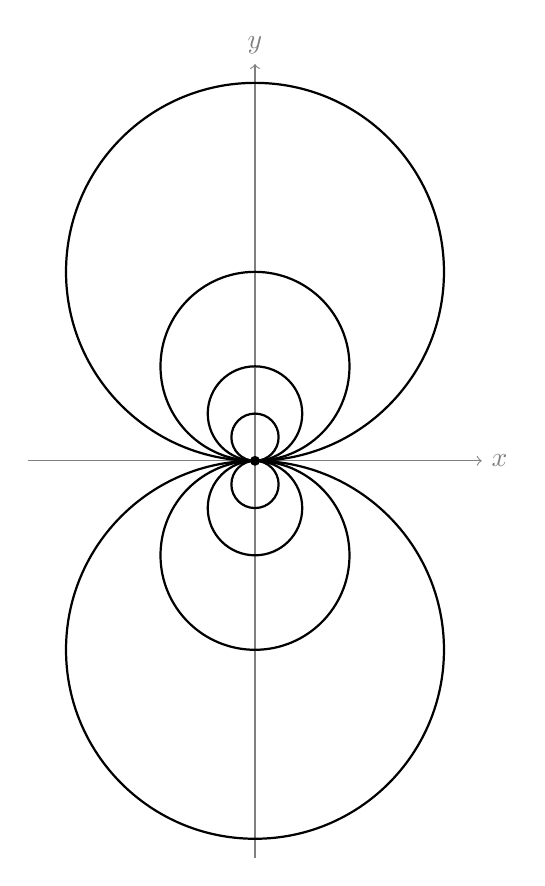
\begin{tikzpicture}[scale=1.2]
	\draw[->, gray] (-2.4,0) -- (2.4,0) node[right] {\( x \)};
	\draw[->, gray] (0,-4.2) -- (0,4.2) node[above] {\( y \)};
	\foreach \R in {0.25, 0.5, 1, 2} {
		\draw[thick] (0,\R) circle (\R);
		\draw[thick] (0,-\R) circle (\R);
	}
	\fill (0,0) circle (1.5pt);
\end{tikzpicture}
\end{center}

% QUESTION 28
\qs{2.5.28}{Solve Laplace's equation inside a rectangle:
\[
	\nabla^{2}u = \frac{\partial^2 u}{\partial x^2} + \frac{\partial^2 u}{\partial y^2} = 0 
\]
subject to the boundary conditions
\begin{alignat*}{3}
	u \!\left( 0,y \right) & = g \!\left( y \right) & \qquad u \!\left( x,0 \right) & = 0 \\
	u \!\left( L,y \right) & = 0 & \qquad u \!\left( x,H \right) & = 0
\end{alignat*}}

Let \( u \!\left( x,y \right) = \phi \!\left( x \right) G \!\left( y \right) \). Substitute into Laplace's equation to find
\[
	G \!\left( y \right)\frac{d^2 \phi}{d x^2} + \phi \!\left( x \right)\frac{d^2 G}{d y^2} = 0 
\]
Divide through by \( \phi \!\left( x \right)G \!\left( y \right) \) and subtract the \( y \) term to find
\[
	\frac{1}{\phi \!\left( x \right)}\frac{d^2 \phi}{d x^2} = -\frac{1}{G \!\left( y \right)}\frac{d^2 G}{d y^2} 
\]
Since our boundary conditions are homogeneous in \( y \), we want the eigenfunctions in that variable to oscillate, so we set both \( x \) and \( y \) terms equal to \( \lambda \):
\[
	\frac{1}{\phi \!\left( x \right)}\frac{d^2 \phi}{d x^2} = -\frac{1}{G \!\left( y \right)}\frac{d^2 G}{d y^2} = \lambda
\]
Suppose that \( \lambda > 0 \). Solve the \( y \) equation first. It is a simple second-order ordinary differential equation solved by
\[
	G \!\left( y \right) = c_{1}\cos\!\left(\sqrt{\lambda}y\right) + c_{2}\sin\!\left(\sqrt{\lambda}y\right) 
\]
Apply the boundary conditions in \( y \). We find
\begin{align*}
	G \!\left( 0 \right) & = c_{1} = 0 \\
	G \!\left( H \right) & = c_{2}\sin\!\left(\sqrt{\lambda}H\right) = 0
\end{align*}
and for a nontrivial solution to emerge, we can require
\[
	\lambda_{n} = \!\left( \frac{n \pi}{H} \right)^{2}, \quad n = 1, 2, ...
\]
which comprise our eigenvalues for this eigenfunction problem. Speaking of which, for \( \lambda > 0 \), we have corresponding eigenfunction
\[
	G \!\left( y \right) = \sin\!\left(\frac{n \pi y}{H}\right) 
\]
In the case where \( \lambda = 0 \), integrate the second derivative twice to find solution
\[
	G \!\left( y \right) = c_{1} + c_{2}y 
\]
Apply boundary conditions to see that only the trivial solution exists:
\begin{align*}
	G \!\left( 0 \right) & = c_{1} = 0 \\
	G \!\left( H \right) & = c_{2}H = 0 \quad \implies \quad c_{2} = 0
\end{align*}
And finally, suppose \( \lambda < 0 \). Then define \( s = -\lambda \), which is positive. Solve
\[
	\frac{1}{G \!\left( y \right)}\frac{d^2 G}{d y^2} = s 
\]
which has solution
\[
	G \!\left( y \right) = c_{1}\cosh\!\left(\sqrt{s}y\right) + c_{2}\sinh\!\left(\sqrt{s}y\right) 
\]
Applying the boundary conditions yields
\begin{align*}
	G \!\left( 0 \right) & = c_{1} = 0 \\
	G \!\left( H \right) & = c_{2}\sinh\!\left(\sqrt{s}H\right) = 0 \quad \implies \quad c_{2} = 0
\end{align*}
which merely produces the trivial solution yet again, enabling us to conclude that in this case, we only have positive eigenvalues. Next we solve the \( x \) problem with
\[
	\phi \!\left( x \right) = a_{1}\cosh\!\left[\frac{n \pi}{H}\!\left( x - L \right)\right] + a_{2}\sinh\!\left[\frac{n \pi}{H}\!\left( x - L \right)\right]
\]
Impose the zero boundary condition in \( x \) to derive our eigenfunction
\[
	\phi \!\left( L \right) = a_{1} = 0 \quad \implies \quad \phi \!\left( x \right) = \sinh\!\left[ \frac{n \pi}{H}\!\left( x - L \right) \right]
\]
Reassembling the product \( \phi \!\left( x \right)G \!\left( y \right) \) and taking the linear combination of all possible solutions, we have
\[
	u \!\left( x,y \right) = \sum^{\infty}_{n=1} A_{n}\sin\!\left(\frac{n \pi y}{H}\right)\sinh\!\left[\frac{n \pi}{H}\!\left( x - L \right)\right]
\]
To determine the coefficients \( A_{n} \), evaluate at \( x = 0 \) and multiply both sides by \( \sin\!\left(m \pi y / H\right) \) to find
\[
	u \!\left( 0,y \right) = \sum^{\infty}_{n=1} A_{n}\sin\!\left(\frac{n \pi y}{H}\right)\sin\!\left(\frac{m \pi y}{H}\right)\sinh\!\left[\frac{n \pi}{H}\!\left( - L \right)\right] = g \!\left( y \right)\sin\!\left(\frac{m \pi y}{H}\right)
\]
Integrate both sides over \( \!\left[ 0,H \right] \), and by orthogonality, all \( n \neq m \) terms will be eliminated, leaving us with
\[
	A_{m}\sinh\!\left[\frac{m \pi}{H}\!\left( -L \right)\right]\underbrace{\int^{H}_{0} \sin^{2}\!\left(\frac{m \pi y}{H}\right) \, dy}_{H / 2} = \int^{H}_{0} g \!\left( y \right)\sin\!\left(\frac{m \pi y}{H}\right) \, dy  
\]
Lastly, isolate \( A_{m} \) to get
\[
	A_{m} = \frac{2}{H \sinh\!\left(m \pi \!\left( -L \right) / H\right)} \int^{H}_{0} g \!\left( y \right)\sin\!\left(\frac{m \pi y}{H}\right) \, dy  
\]

% QUESTION 29
\qs{2.5.29}{Solve Laplace's equation inside a circle of radius \( a \),
\[
	\nabla^{2}u = \frac{1}{r}\frac{\partial }{\partial r}\!\left( r \frac{\partial u}{\partial r} \right) + \frac{1}{r^{2}}\frac{\partial^2 u}{\partial \theta^2} = 0, 
\]
subject to the boundary condition
\[
	u \!\left( a,\theta \right) = f \!\left( \theta \right) 
\]}
Let \( u \!\left( r,\theta \right) = \phi \!\left( \theta \right)G \!\left( r \right) \). We require periodic boundary conditions in \( \theta \) that ensure continuity of \( \phi \!\left( \theta \right) \); they are
\begin{align*}
	\phi \!\left( -\pi \right) & = \phi \!\left( \pi \right) \\
	\frac{d \phi}{d \theta}\!\left( -\pi \right) & = \frac{d \phi}{d \theta}\!\left( \pi \right)
\end{align*}
Now substitute \( \phi \!\left( \theta \right) G \!\left( r \right) \) into Laplace's equation:
\[
	\nabla^{2}u = \frac{\phi \!\left( \theta \right)}{r}\frac{d }{d r}\!\left( r \frac{d G}{d r} \right) + \frac{G \!\left( r \right)}{r^{2}}\frac{d^2 \phi}{d \theta^2} = 0
\]
Divide through by \( \displaystyle{\frac{1}{r^{2}}}\phi \!\left( \theta \right)G \!\left( r \right) \) and subtract the \( \theta \) equation to get
\[
	\frac{r}{G \!\left( r \right)}\frac{d }{d r}\!\left( r \frac{d G}{d r} \right) = -\frac{1}{\phi \!\left( \theta \right)}\frac{d^2 \phi}{d \theta^2} = \lambda
\]
where, since we require oscillation in \( \theta \) to satisfy the periodic boundary conditions, we set equal to \( \lambda \). So let's solve that eigenvalue problem; its solution is (assuming \( \lambda > 0 \))
\[
	\phi \!\left( \theta \right) = c_{1}\cos\!\left(\sqrt{\lambda}\theta\right) + c_{2}\sin\!\left(\sqrt{\lambda}\theta\right)
\]
Imposing the boundary conditions produces
\begin{align*}
	\phi \!\left( -\pi \right) & = c_{1}\cos\!\left(\sqrt{\lambda}\pi\right) - c_{2}\sin\!\left(\sqrt{\lambda}\pi\right) \\
	\phi \!\left( \pi \right) & = c_{1}\cos\!\left(\sqrt{\lambda}\pi\right) + c_{2}\sin\!\left(\sqrt{\lambda}\pi\right) \\ 
	\implies 0 & = 2c_{2}\sin\!\left(\sqrt{\lambda}\pi\right) \\
	\frac{d \phi}{d \theta}\!\left( -\pi \right) & = c_{1}\sqrt{\lambda}\sin\!\left(\sqrt{\lambda}\pi\right) + c_{2}\sqrt{\lambda}\cos\!\left(\sqrt{\lambda}\pi\right) \\
	\frac{d \phi}{d \theta}\!\left( \pi \right) & = -c_{1}\sqrt{\lambda}\sin\!\left(\sqrt{\lambda}\pi\right) + c_{2}\sqrt{\lambda}\cos\!\left(\sqrt{\lambda}\pi\right) \\
	\implies 0 & = c_{1}\sqrt{\lambda}\sin\!\left(\sqrt{\lambda}\pi\right)
\end{align*}
where a nontrivial solution exists when
\[
	\lambda_{n} = n^{2}, \quad n = 1, 2, ...
\]
Thus our eigenfunctions are
\[
	\phi \!\left( \theta \right) = \sin\!\left(n \theta\right), \cos\!\left(n \theta\right) 
\]
Next we solve the \( r \) equation (first assuming \( \lambda > 0 \)), which we now write as 
\[
	\frac{r}{G}\frac{d }{d r}\!\left( r \frac{d G}{d r} \right) = n^{2} \quad \implies \quad r^{2}\frac{d^2 G}{d r^2} + r \frac{d G}{d r} - n^{2}G = 0 
\]
to make its equidimensional form more apparent. One more boundedness condition is needed: require \( \abs{u \!\left( 0,\theta \right)} < \infty \), and particularly, \( \abs{G \!\left( 0 \right)} < \infty \). In other words, \( u \) must be finite at the origin. Let \( G \!\left( r \right) = r^{p} \). Solve as 
\[
	p \!\left( p - 1 \right)r^{p} + p r^{p} - n^{2} r^{p} = 0 \quad \implies \quad p^{2} - n^{2} = 0 \quad \implies \quad p = \pm n 
\]
which leaves us with solution
\[
	G \!\left( r \right) = a_{1}r^{n} + a_{2}r^{-n} 
\]
Applying the boundedness condition, we can conclude that \( a_{2} = 0 \) and eigenfunction
\[
	G \!\left( r \right) = r^{n} 
\]
In the second case where \( \lambda = 0 \), we endeavor to solve
\[
	\frac{r}{G}\frac{d }{d r}\!\left( r \frac{d G}{d r} \right) = 0 
\]
Dividing by \( r / G \) and integrating twice, derive solution
\[
	G \!\left( r \right) = b_{1} + b_{2}\ln\!\left(r\right) 
\]
and applying the boundedness condition once more forces \( b_{2} = 0 \), leaving the constant eigenfunction.

Taking the product of the eigenfunctions and assembling their linear combination, we have solution
\[
	u \!\left( r,\theta \right) = C + \sum^{\infty}_{n=1} A_{n}r^{n}\cos\!\left(n \theta\right) + \sum^{\infty}_{n=1} B_{n}r^{n}\sin\!\left(n \theta\right), \quad -\pi \le \theta \le \pi
\]
For our last (non-homogeneous!) boundary condition, set \( r = a \) and write
\[
	u \!\left( a,\theta \right) = C + \sum^{\infty}_{n=1} A_{n}a^{n}\cos\!\left(n \theta\right) + \sum^{\infty}_{n=1} B_{n}a^{n}\sin\!\left(n \theta\right) = f \!\left( \theta \right)
\]
Multiply through first by \( \cos\!\left(m \theta\right) \), integrate. Repeat with \( \sin\!\left(m \theta\right) \) and integrate. Lastly, for the constant term, no multiplication -- simply integrate over \( \!\left[ -\pi,\pi \right] \). Orthogonality produces for us the coefficients
\begin{align*}
	C & = \frac{1}{2 \pi}\int^{\pi}_{-\pi} f \!\left( \theta \right) \, d \theta \\
	A_{n}a^{n} & = \frac{1}{\pi}\int^{\pi}_{-\pi} f \!\left( \theta \right)\cos\!\left(n \theta\right) \, d \theta \\ 
	B_{n}a^{n} & = \frac{1}{\pi}\int^{\pi}_{-\pi} f \!\left( \theta \right)\sin\!\left(n \theta\right) \, d \theta 
\end{align*}



\newpage
\section{\textsf{3 - Fourier Series}}
\subsection{\textsf{3.2 - Statement of Convergence Theorem}}

% QUESTION 1
\qs{3.2.1}{For the following functions, sketch the Fourier series of \( f \!\left( x \right) \) (on the interval \( -L \le x \le L \). Compare \( f \!\left( x \right) \) to its Fourier series:
\begin{enumerate}[label=(\alph*)]
	\item \( f \!\left( x \right) = 1 \)
	\item \( f \!\left( x \right) = x^{2} \)
	\item \( f \!\left( x \right) = 1 + x \)
	\item \( f \!\left( x \right) = e^{x} \)
	\item \( f \!\left( x \right) = \begin{cases}
		x & x < 0 \\
		2x & x > 0 
	\end{cases} \)
	\item \( f \!\left( x \right) = \begin{cases}
		0 & x < 0 \\
		1 + x & x > 0 
	\end{cases} \)
	\item \( f \!\left( x \right) = \begin{cases}
		x & x < L / 2 \\
		0 & x > L / 2 
	\end{cases} \)
\end{enumerate}}

\begin{enumerate}[label=(\alph*)]
	\item 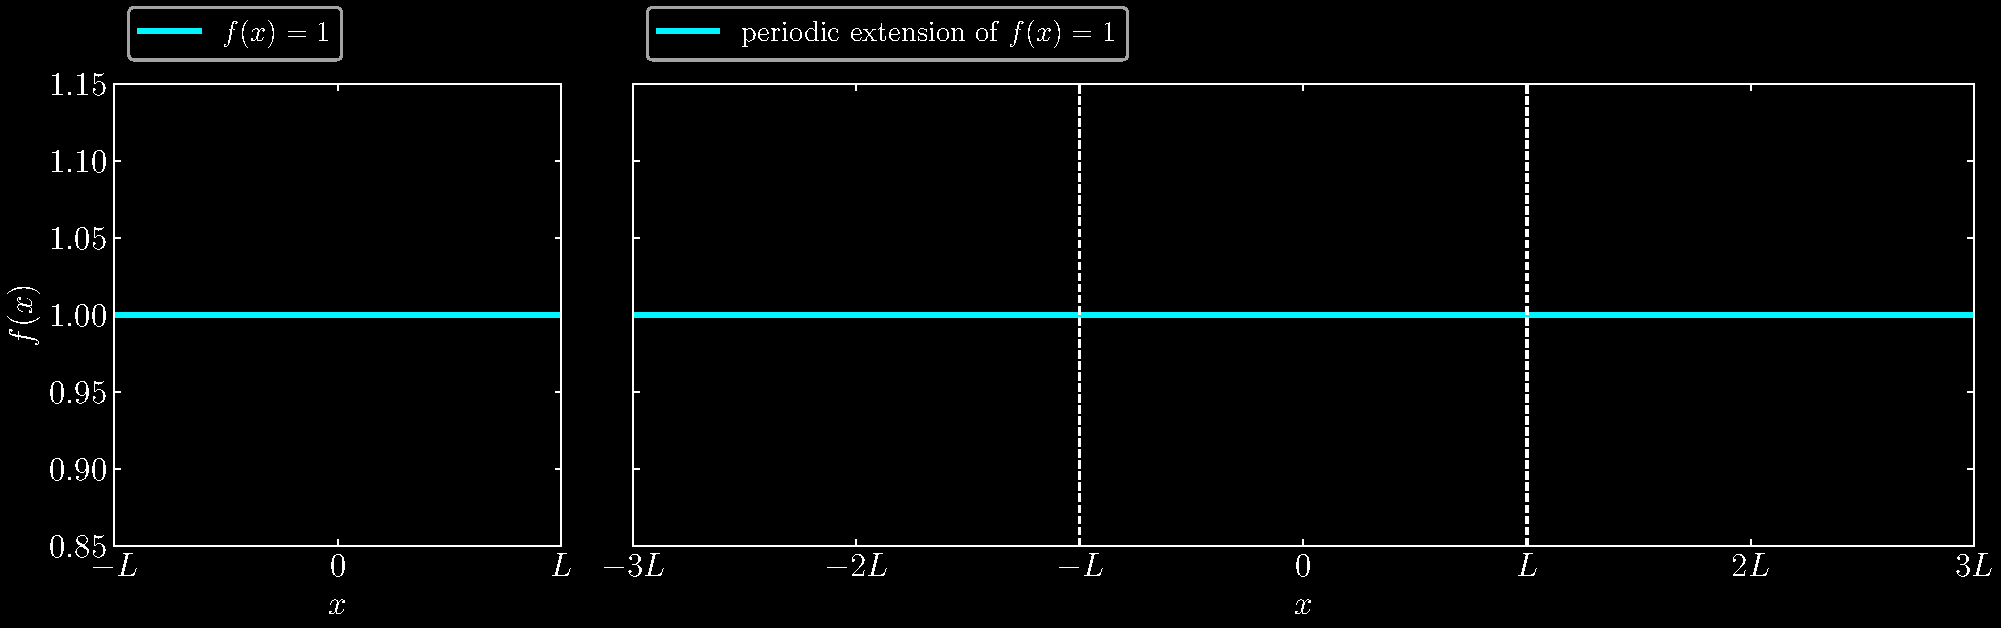
\includegraphics[width=0.9\textwidth]{../chap3/sec3.2/chap3sec3.2ex1a.pdf}
	\item 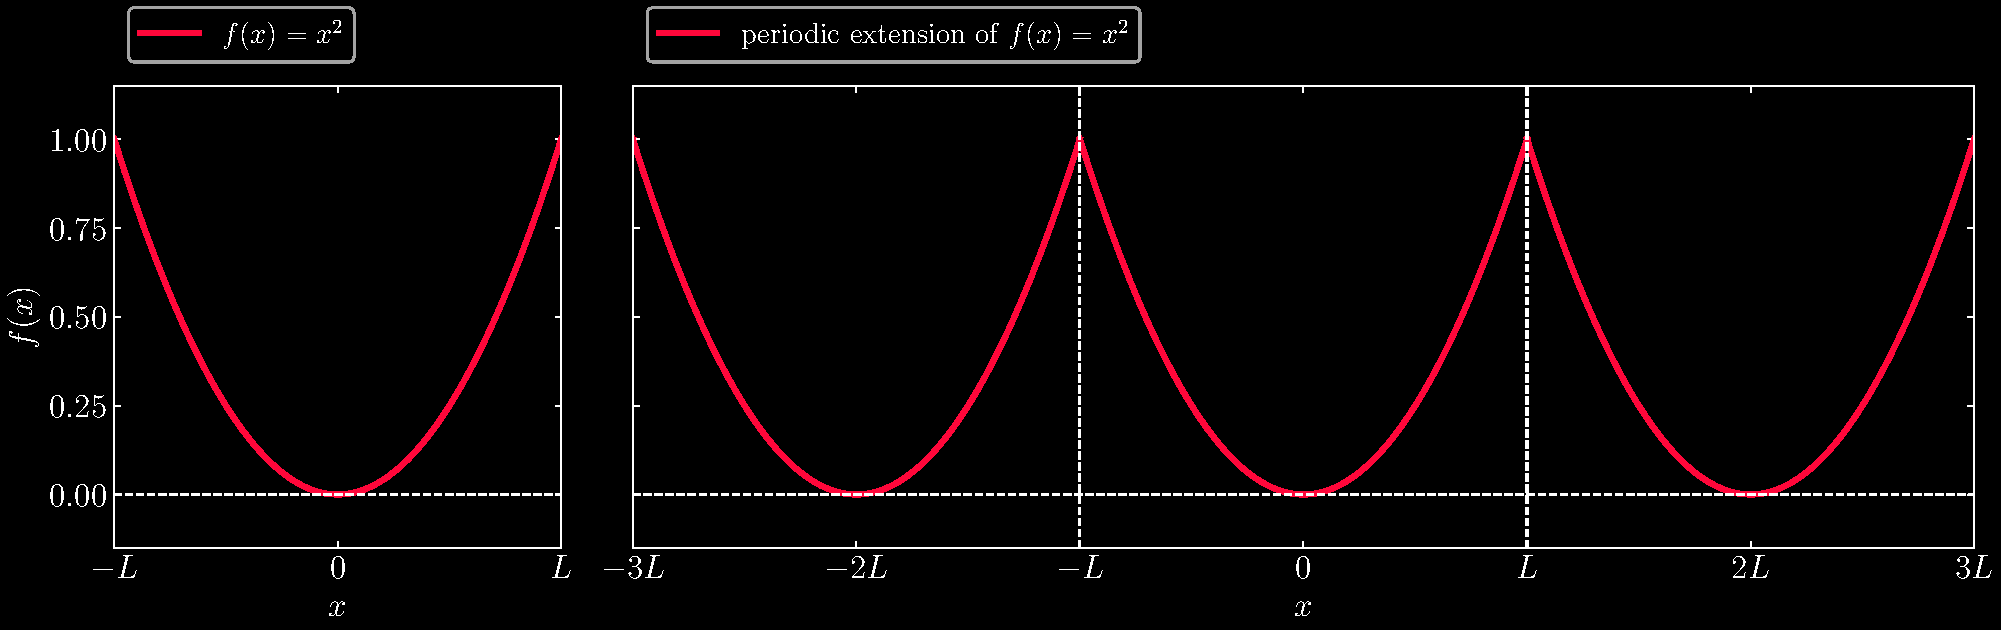
\includegraphics[width=0.9\textwidth]{../chap3/sec3.2/chap3sec3.2ex1b.pdf}
	\item 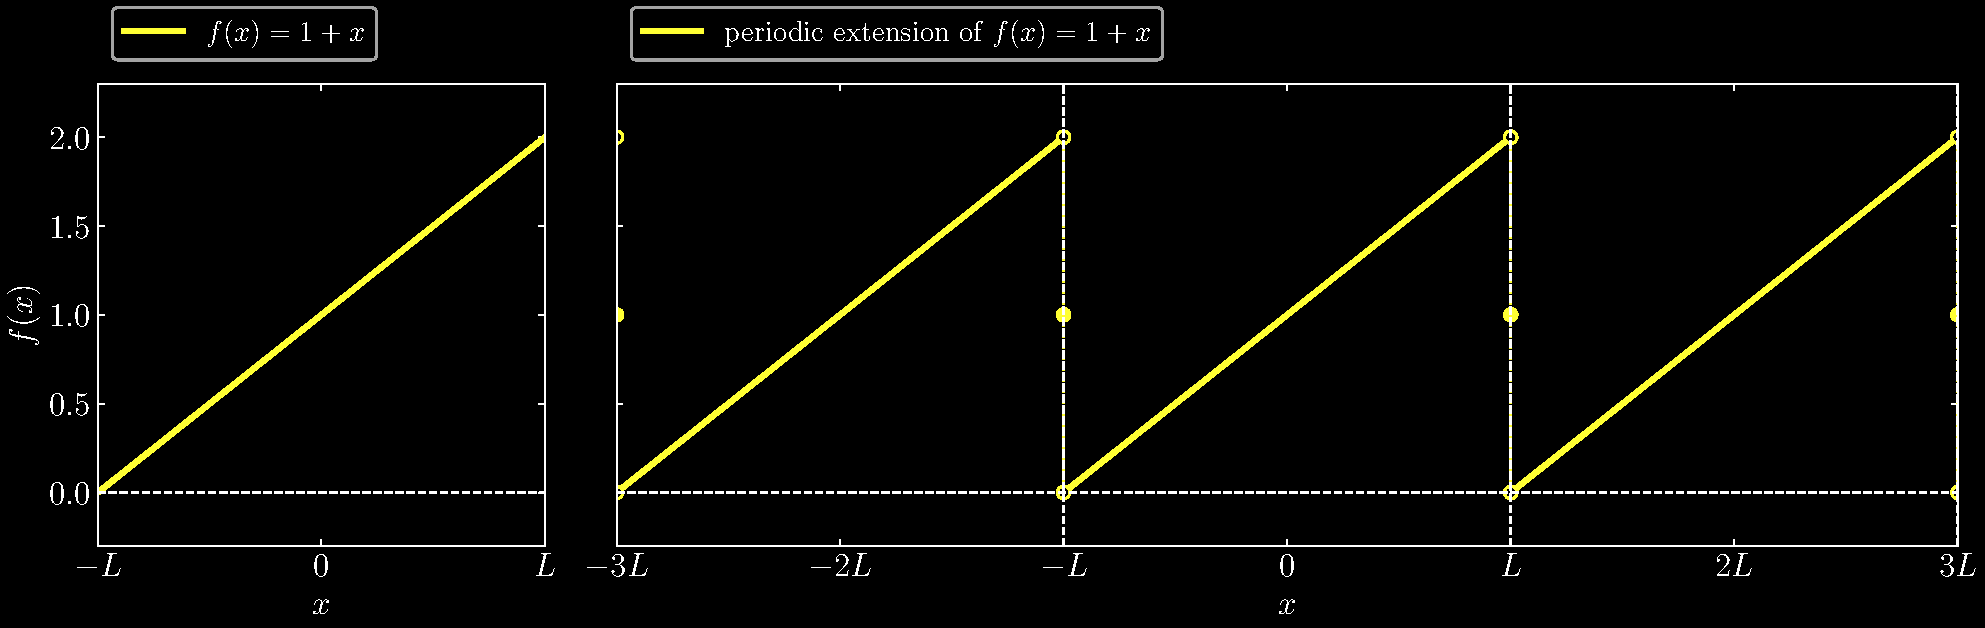
\includegraphics[width=0.9\textwidth]{../chap3/sec3.2/chap3sec3.2ex1c.pdf}
	\item 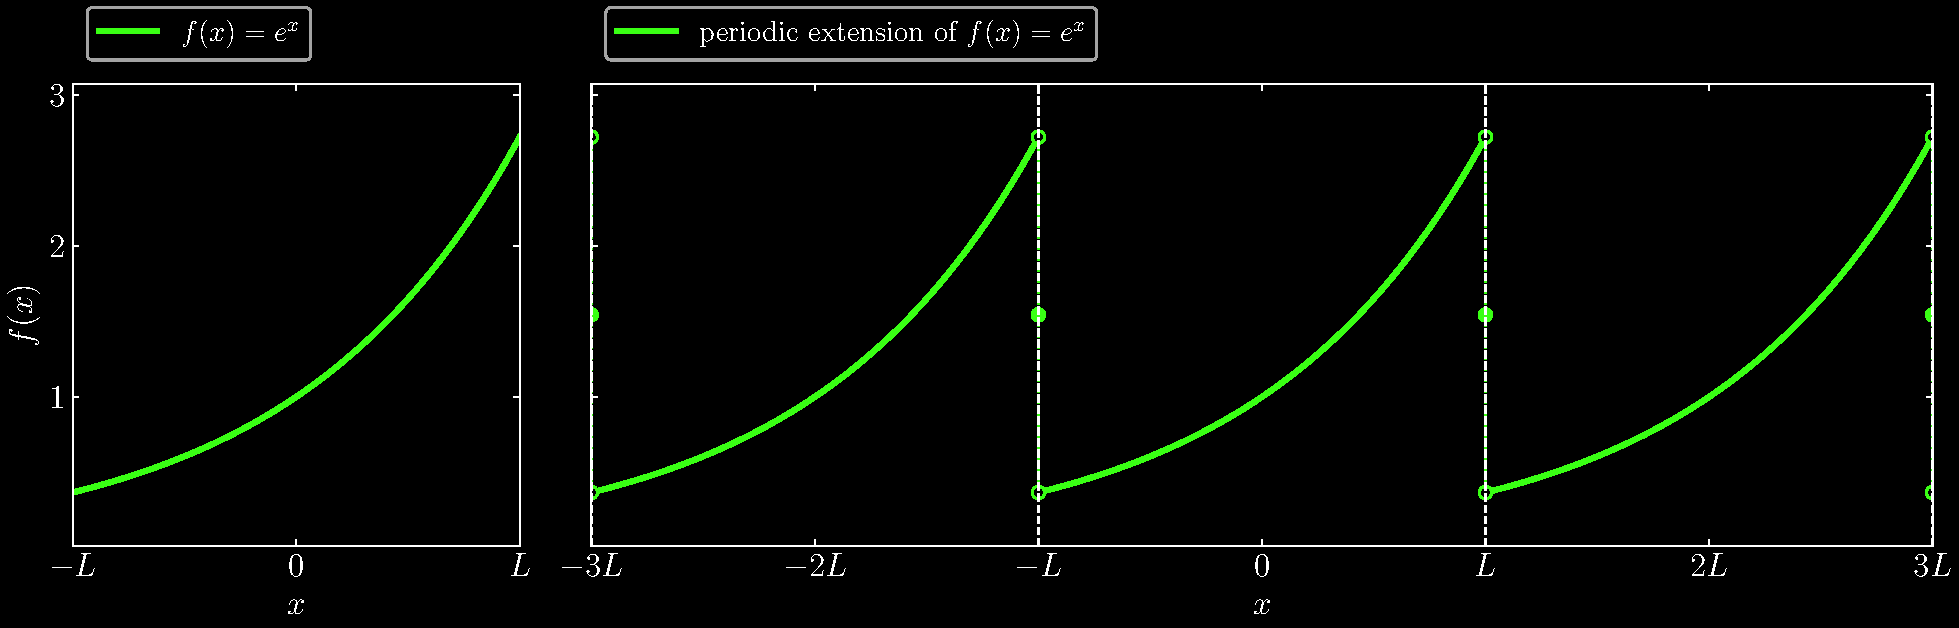
\includegraphics[width=0.9\textwidth]{../chap3/sec3.2/chap3sec3.2ex1d.pdf}
	\item 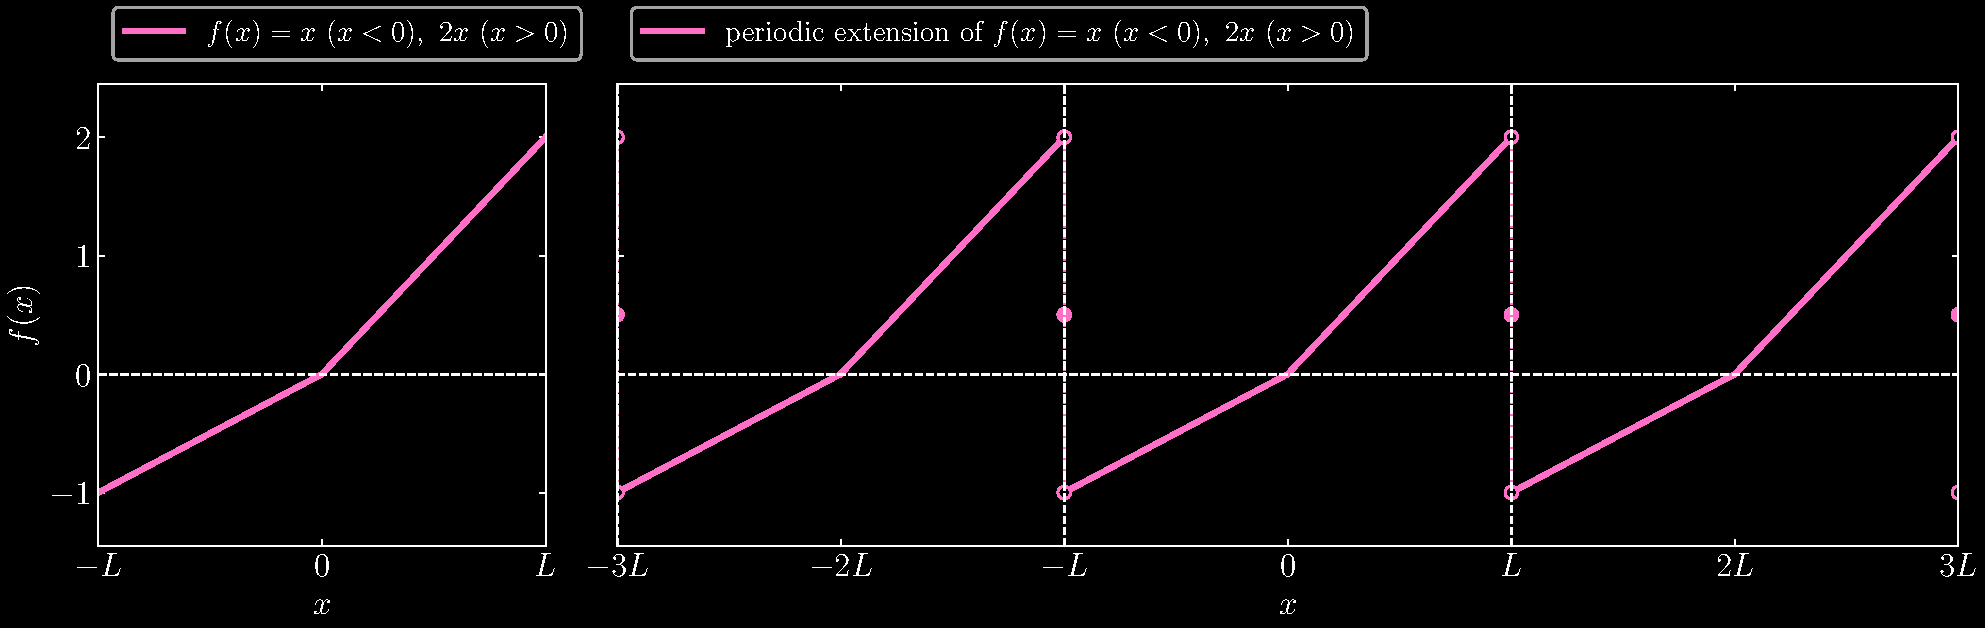
\includegraphics[width=0.9\textwidth]{../chap3/sec3.2/chap3sec3.2ex1e.pdf}
	\item 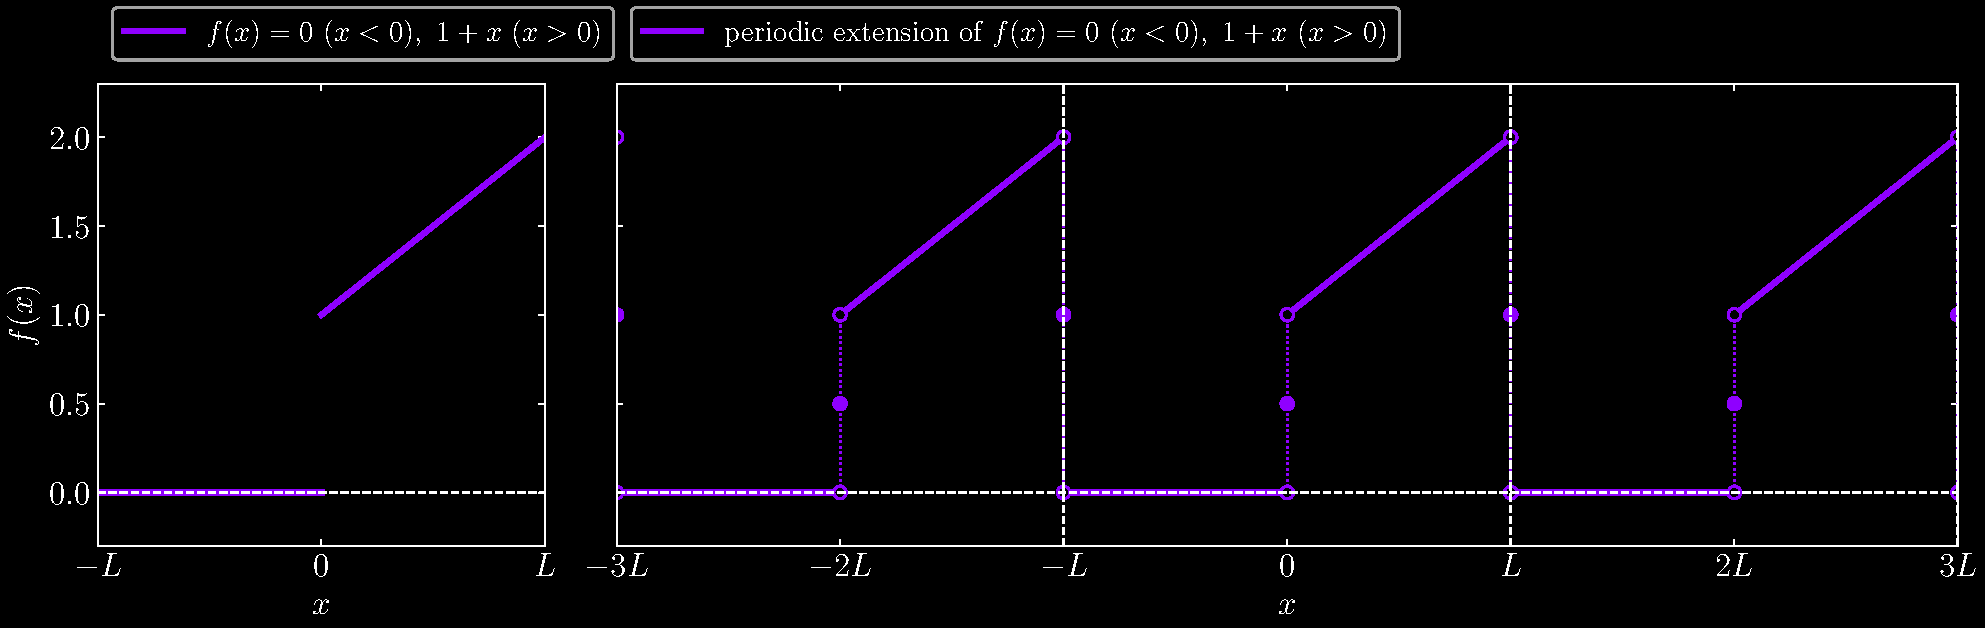
\includegraphics[width=0.9\textwidth]{../chap3/sec3.2/chap3sec3.2ex1f.pdf}
	\item 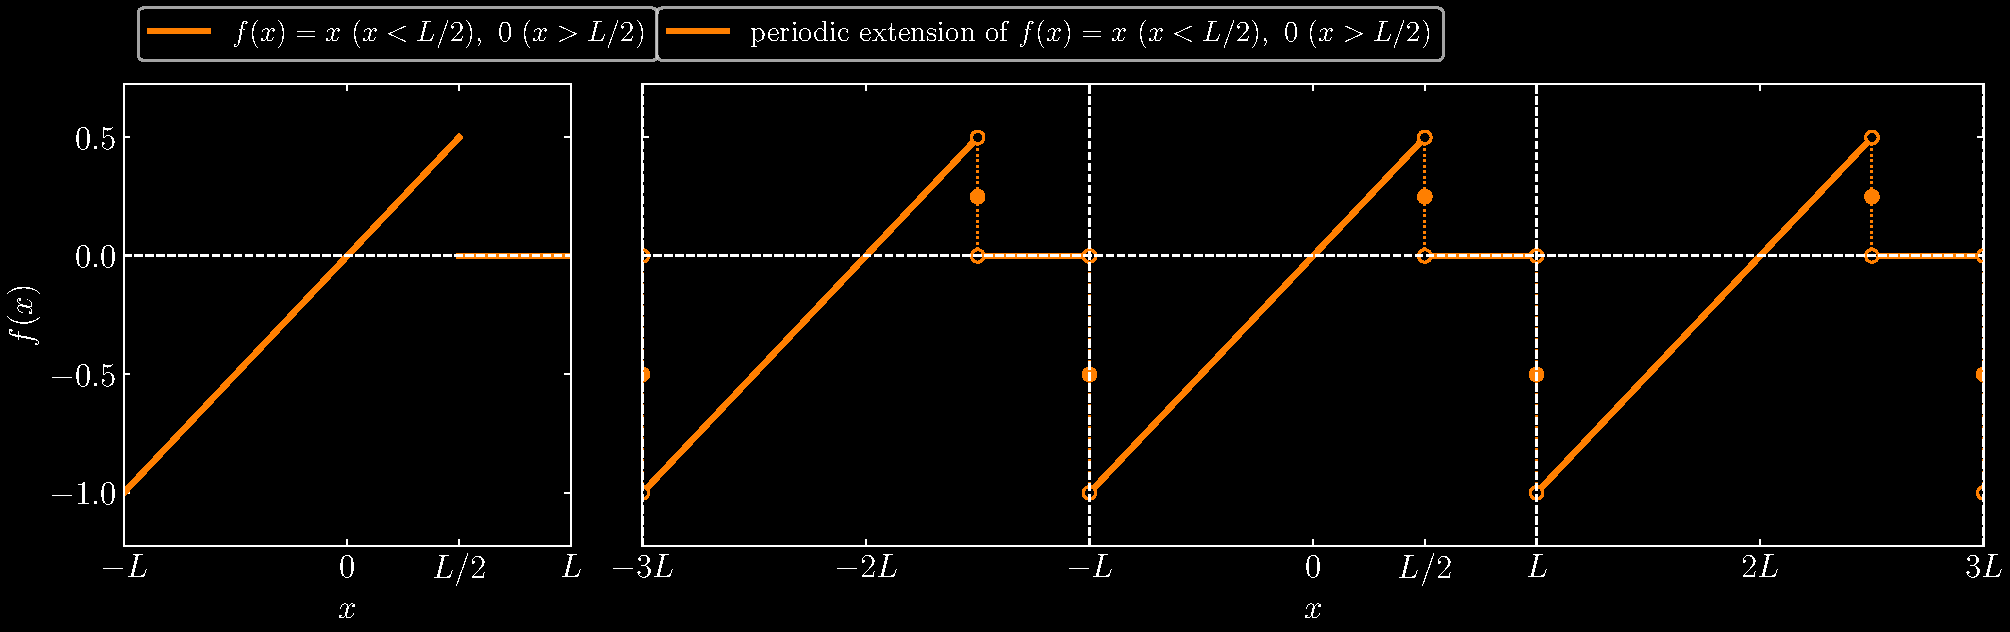
\includegraphics[width=0.9\textwidth]{../chap3/sec3.2/chap3sec3.2ex1g.pdf}
\end{enumerate}

% QUESTION 2
\qs{3.2.2}{For the following functions, sketch the Fourier series of \( f \!\left( x \right) \) (on the interval \( -L \le x \le L \) and determine the Fourier coefficients:
\begin{enumerate}[label=(\alph*)]
	\item \( f \!\left( x \right) = x \)
	\item \( f \!\left( x \right) = e^{-x} \)
	\item \( f \!\left( x \right) = \displaystyle{\sin\!\left(\frac{\pi x}{L}\right)} \)
	\item \( f \!\left( x \right) = \begin{cases}
		0 & x < 0 \\
		x & x > 0 
	\end{cases} \)
	\item \( f \!\left( x \right) = \begin{cases}
		1 & \abs{x} < L / 2 \\
		0 & \abs{x} > L / 2 
	\end{cases} \)
	\item \( f \!\left( x \right) = \begin{cases}
		0 & x < 0 \\
		1 & x > 0 
	\end{cases} \)
	\item \( f \!\left( x \right) = \begin{cases}
		1 & x < 0 \\
		2 & x > 0 
	\end{cases} \)
\end{enumerate}}

\begin{enumerate}[label=(\alph*)]
	\item Since \( f \!\left( x \right) \) is odd, we only have non-zero coefficients for the Fourier sine series:
	\begin{align*}
		b_{n} & = \frac{1}{L}\int^{L}_{-L} x \sin\!\left(\frac{n \pi x}{L}\right) \, dx \\
		 & = \frac{1}{L}\!\left[ -\frac{L}{n \pi}x \cos\!\left(\frac{n \pi x}{L}\right)\Big|^{L}_{-L} + \frac{L}{n \pi}\int^{L}_{-L} \cos\!\left(\frac{n \pi x}{L}\right) \, dx \right] \\ 
		 & = -\frac{2L}{n \pi}\cos\!\left(n \pi\right) \\
		 & = \frac{2L}{n \pi}\!\left( -1 \right)^{n + 1}
	\end{align*}
	\begin{center}
	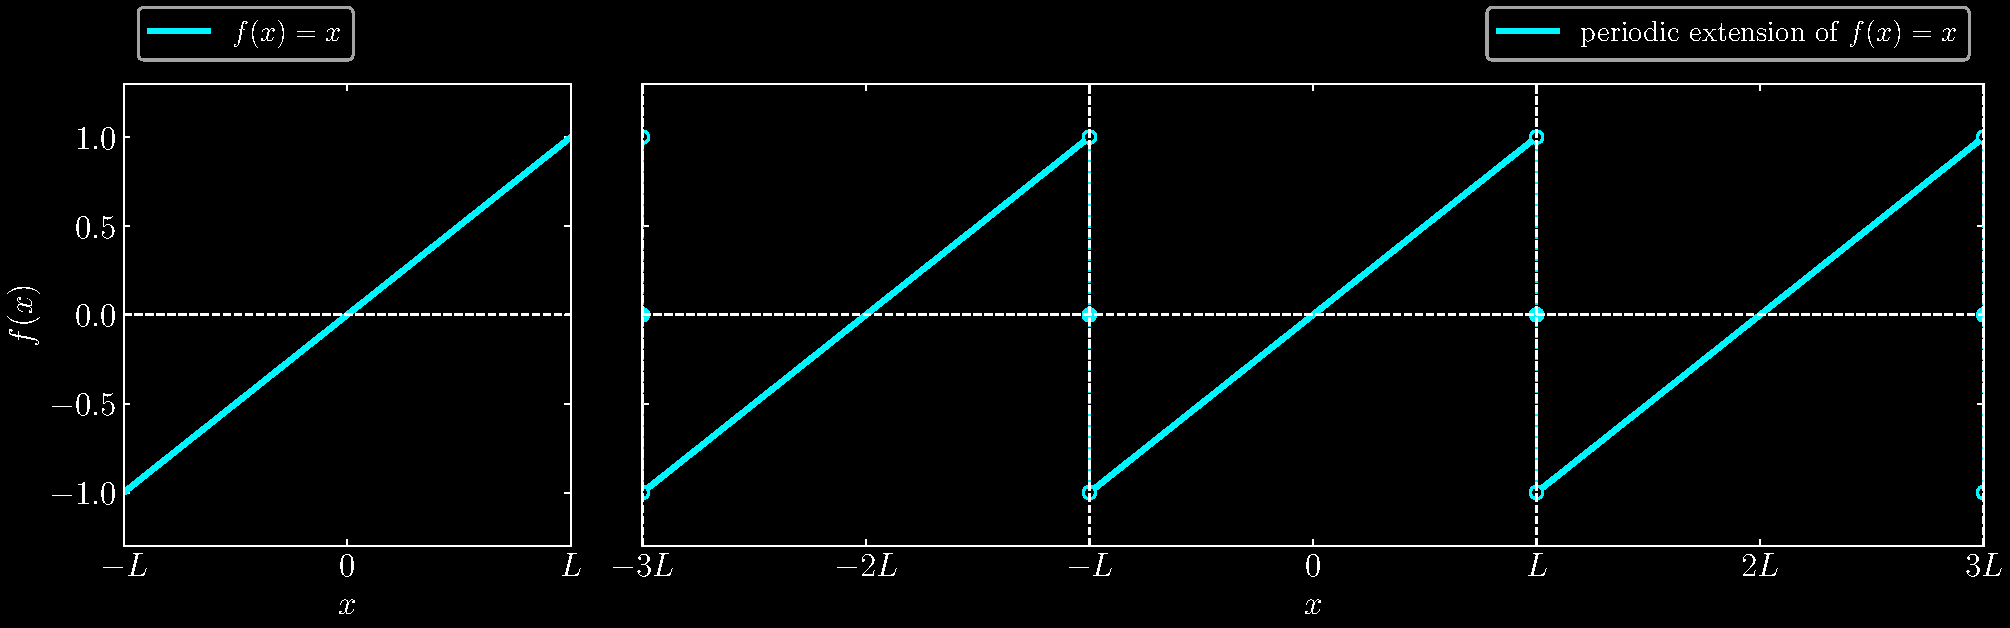
\includegraphics[width=0.9\textwidth]{../chap3/sec3.2/chap3sec3.2ex2a.pdf}
	\end{center}
	\item \begin{align*}
		a_{0} & = \frac{1}{2L}\int^{L}_{-L} e^{-x} \, dx \\
		 & = \frac{1}{2L}\!\left( e^{L} - e^{-L} \right) \\
		 & = \frac{1}{L}\sinh\!\left(L\right) \\
		a_{n} & = \frac{1}{L}\int^{L}_{-L} e^{-x}\cos\!\left(\frac{n \pi x}{L}\right) \, dx \\
		      & = \frac{1}{L}\left[\frac{e^{-x}\left(\frac{n\pi}{L}\sin\!\left(\frac{n \pi x}{L}\right) - \cos\!\left(\frac{n \pi x}{L}\right)\right)}{1+\frac{n^2\pi^2}{L^2}}\right]^{L}_{-L} \\
      & = \frac{(-1)^n\left(e^{L}-e^{-L}\right)}{L\left(1+\frac{n^2\pi^2}{L^2}\right)} \\
      & = \frac{2(-1)^n L\sinh\!\left( L \right)}{L^2+n^2\pi^2} \\
		b_{n} & = \frac{1}{L}\int^{L}_{-L} e^{-x}\sin\!\left(\frac{n \pi x}{L}\right) \, dx \\
		      & = -\frac{1}{L}\left[\frac{e^{-x}\left(\sin\!\left(\frac{n \pi x}{L}\right) + \frac{n\pi}{L}\cos\!\left(\frac{n \pi x}{L}\right)\right)}{1+\frac{n^2\pi^2}{L^2}}\right]^{L}_{-L} \\
      		      & = \frac{n\pi(-1)^n\left(e^{L}-e^{-L}\right)}{L^2\left(1+\frac{n^2\pi^2}{L^2}\right)} \\
      		      & = \frac{2(-1)^n\, n\pi \sinh\!\left(L\right)}{L^2+n^2\pi^2}
	\end{align*}
	\begin{center}
	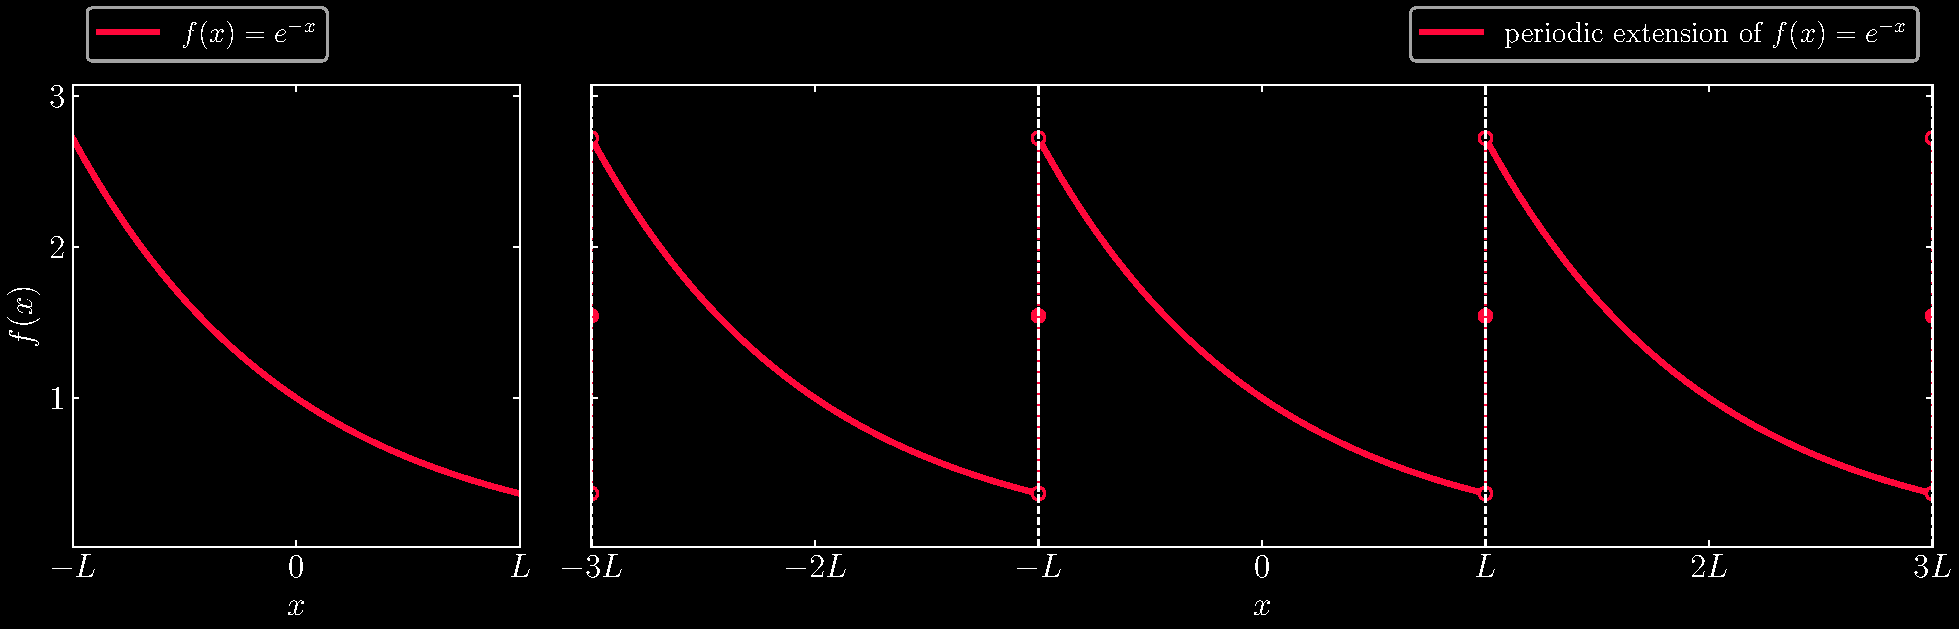
\includegraphics[width=0.9\textwidth]{../chap3/sec3.2/chap3sec3.2ex2b.pdf}
	\end{center}
	\item Since \( f \!\left( x \right) \) is odd, \( a_{0} = 0 \). By orthogonality, \( a_{n} = 0 \) for all \( n \), and \( b_{n} = 0 \), \( n \neq 1 \). We are left with
	\begin{align*}
		b_{1} & = \frac{1}{L}\int^{L}_{-L} \sin^{2}\!\left(\frac{\pi x}{L}\right) \, dx \\
		 & = 1
	\end{align*}
	\begin{center}
	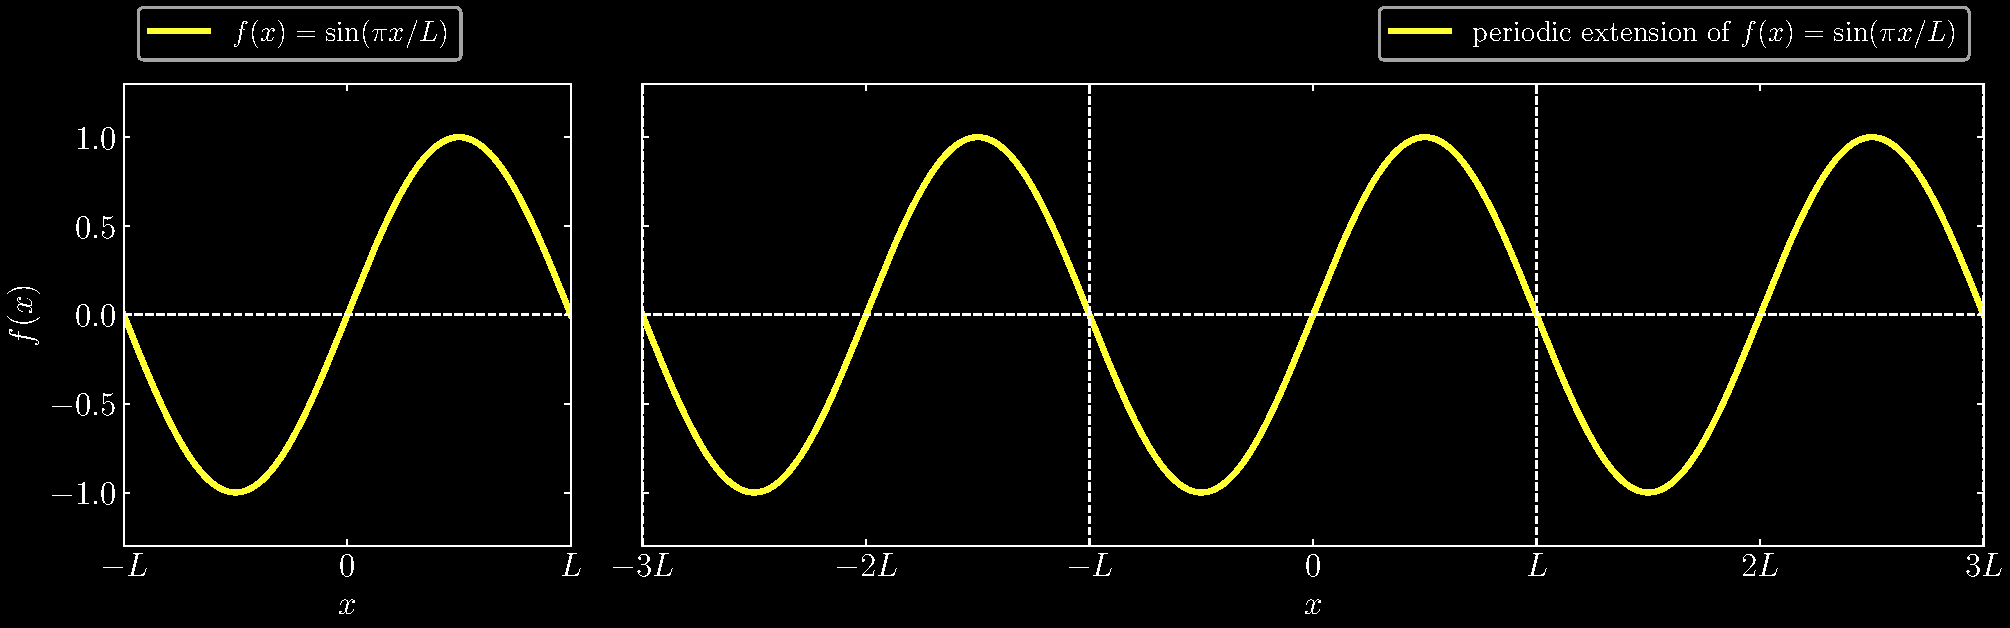
\includegraphics[width=0.9\textwidth]{../chap3/sec3.2/chap3sec3.2ex2c.pdf}
	\end{center}
	\item \begin{align*}
		a_{0} & = \frac{1}{2L}\int^{L}_{0} x \, dx \\
		 & = \frac{L}{4} \\
		a_{n} & = \frac{1}{L}\int^{L}_{0} x \cos\!\left(\frac{n \pi x}{L}\right) \, dx \\
      & = \frac{1}{L}\left[\frac{L}{n\pi}\,x\sin\!\left(\frac{n \pi x}{L}\right)\Big|^{L}_{0} - \frac{L}{n\pi}\int^{L}_{0} \sin\!\left(\frac{n \pi x}{L}\right) \, dx\right] \\
      & = \frac{1}{L}\cdot\frac{L^2}{n^2\pi^2}\cos\!\left(\frac{n \pi x}{L}\right)\Big|^{L}_{0} \\
      & = \frac{L}{n^2\pi^2}\left((-1)^n - 1\right) \\
		b_{n} & = \frac{1}{L}\int^{L}_{0} x \sin\!\left(\frac{n \pi x}{L}\right) \, dx \\
		      & = \frac{1}{L}\left[ -\frac{L}{n \pi}\,x \cos\!\left(\frac{n \pi x}{L}\right)\Big|^{L}_{0} + \frac{L}{n \pi}\int^{L}_{0} \cos\!\left(\frac{n \pi x}{L}\right) \, dx \right] \\
      & = \frac{1}{L}\left[ -\frac{L^2(-1)^n}{n \pi} + \frac{L^2}{n^2 \pi^2}\sin\!\left(\frac{n \pi x}{L}\right)\Big|^{L}_{0} \right] \\
      & = \frac{L(-1)^{n+1}}{n\pi}
	\end{align*}
	\begin{center}
	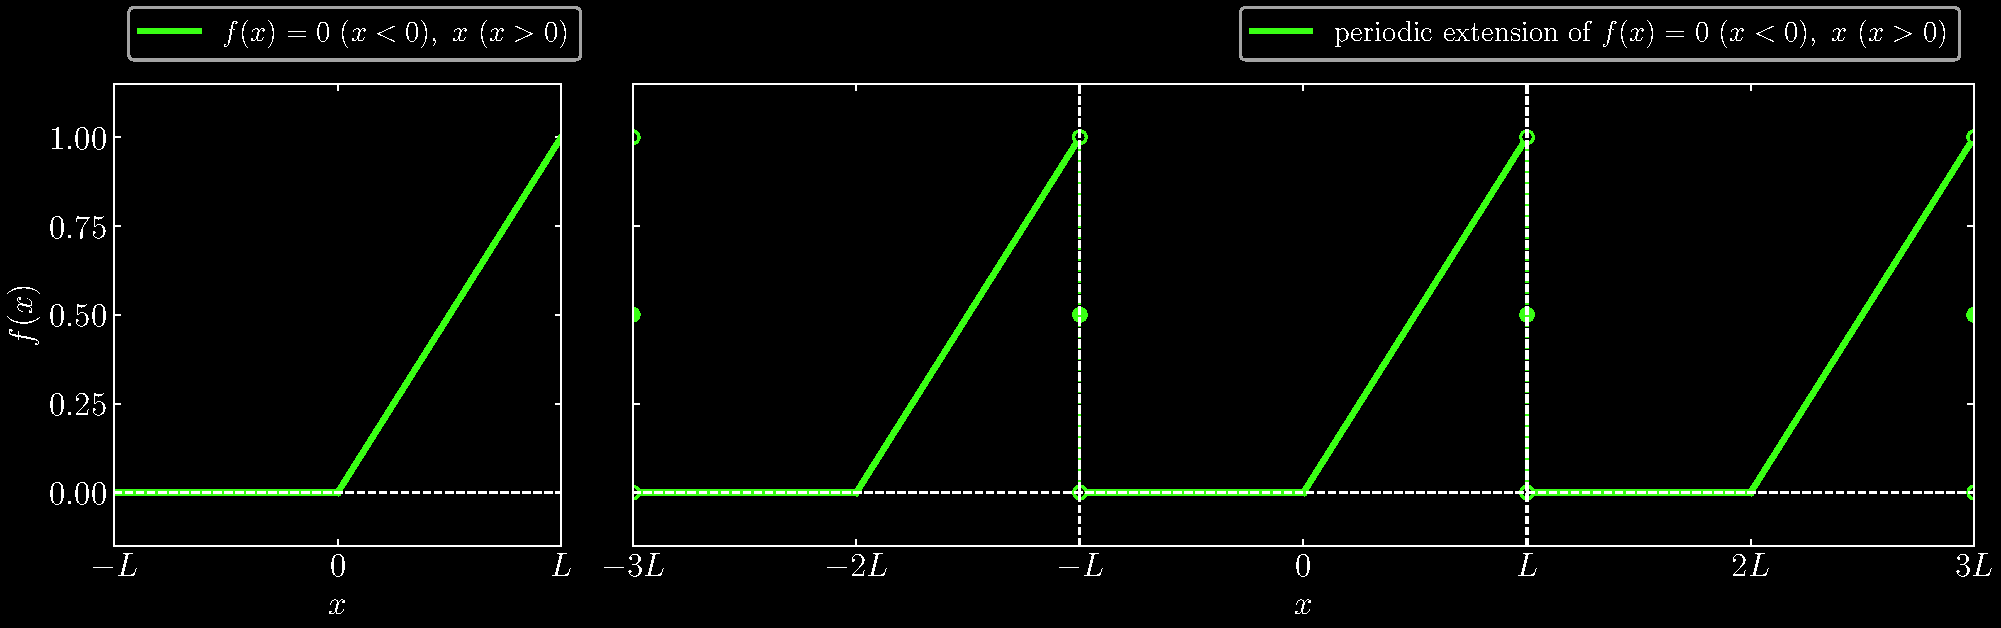
\includegraphics[width=0.9\textwidth]{../chap3/sec3.2/chap3sec3.2ex2d.pdf}
	\end{center}
	\item Since \( f \!\left( x \right) \) is even, the \( b_{n} \) coefficients vanish.
	\begin{align*}
		a_{0} & = \frac{1}{2L}\int^{L/2}_{-L/2}  \, dx \\
		 & = \frac{1}{2} \\ 
		a_{n} & = \frac{1}{L}\int^{L/2}_{-L/2} \cos\!\left(\frac{n \pi x}{L}\right) \, dx \\
		      & = \frac{1}{n \pi}\sin\!\left(\frac{n \pi x}{L}\right)\Big|^{L/2}_{-L/2} \\
		      & = \frac{2}{n \pi}\sin\!\left(\frac{n \pi}{2}\right) \\
		a_{2m - 1} & = \frac{2}{\!\left( 2m - 1 \right)\pi}\!\left( -1 \right)^{m + 1}
	\end{align*}
	where in the last line we change the index to reflect the fact that \( a_{n} = 0 \) for even \( n \).
	\begin{center}
	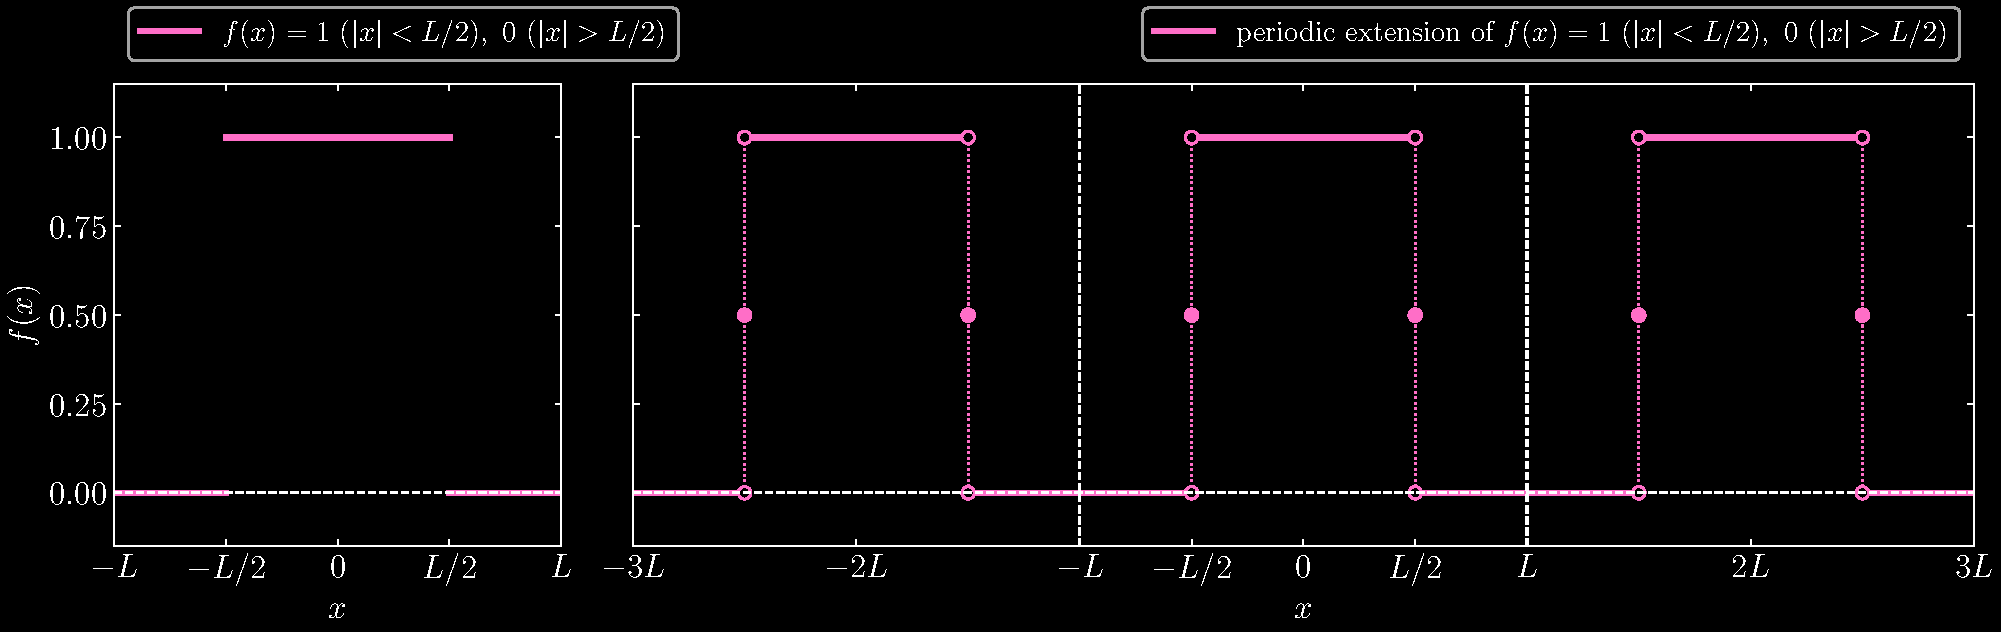
\includegraphics[width=0.9\textwidth]{../chap3/sec3.2/chap3sec3.2ex2e.pdf}
	\end{center}
	\item One intuitive observation is to see that \( f \!\left( x \right) \) is equal to
	\[
		f \!\left( x \right) = \frac{1}{2} + \frac{1}{2}\text{sgn}\!\left( x \right)
	\]
	which adds an odd function to a constant, rendering the \( a_{n} \) coefficients for \( n \ge 1 \) zero.
	\begin{align*}
		a_{0} & = \frac{1}{2L}\int^{L}_{0}  \, dx \\
		 & = \frac{1}{2} \\ 
		b_{n} & = \frac{1}{L}\int^{L}_{0} \sin\!\left(\frac{n \pi x}{L}\right) \, dx \\
		      & = -\frac{1}{n \pi}\cos\!\left(\frac{n \pi x}{L}\right)\Big|^{L}_{0} \\
      & = \frac{1 - (-1)^n}{n \pi}
	\end{align*}
	\begin{center}
	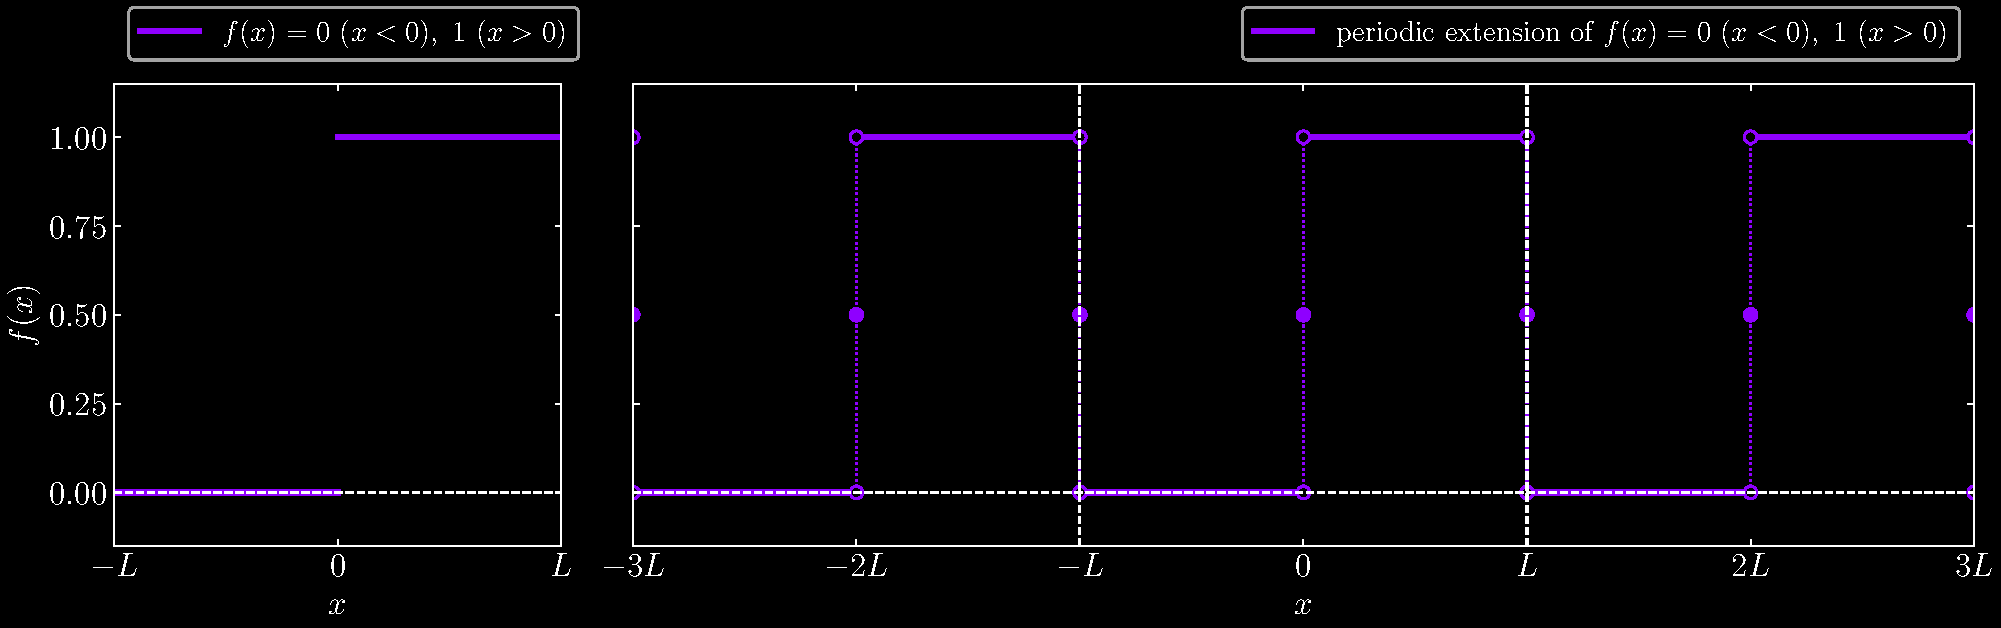
\includegraphics[width=0.9\textwidth]{../chap3/sec3.2/chap3sec3.2ex2f.pdf}
	\end{center}
	\item Here, the step function \( f \!\left( x \right) \) differs from the previous example only by an upward vertical shift of 1. We can equivalently write
	\[
		f \!\left( x \right) = \frac{3}{2} + \frac{1}{2}\text{sgn}\!\left( x \right)
	\]
	which, once more, is a constant added by an odd  function. Therefore the \( a_{n} \) coefficients remain zero, while the \( a_{0} \) coefficient simply is added by 1, which we can verify by
	\[
		a_{0} = \frac{1}{2L}\!\left[ \int^{0}_{-L}  \, dx + \int^{L}_{0} 2 \, dx \right] = \frac{3}{2}
	\]
	The \( b_{n} \) coefficients remain unchanged. The quick way to see this is by exploiting the oddness of sine:
	\begin{align*}
		b_{n} & = \frac{1}{L}\!\left[ \underbrace{\int^{0}_{-L} \sin\!\left(\frac{n \pi x}{L}\right) \, dx}_{= -\int^{L}_{0} \sin\!\left(\frac{n \pi x}{L}\right) \, dx} + 2 \int^{L}_{0} \sin\!\left(\frac{n \pi x}{L}\right) \, dx \right] \\
		 & = \frac{1}{L}\int^{L}_{0} \sin\!\left(\frac{n \pi x}{L}\right) \, dx
	\end{align*}
	\begin{center}
	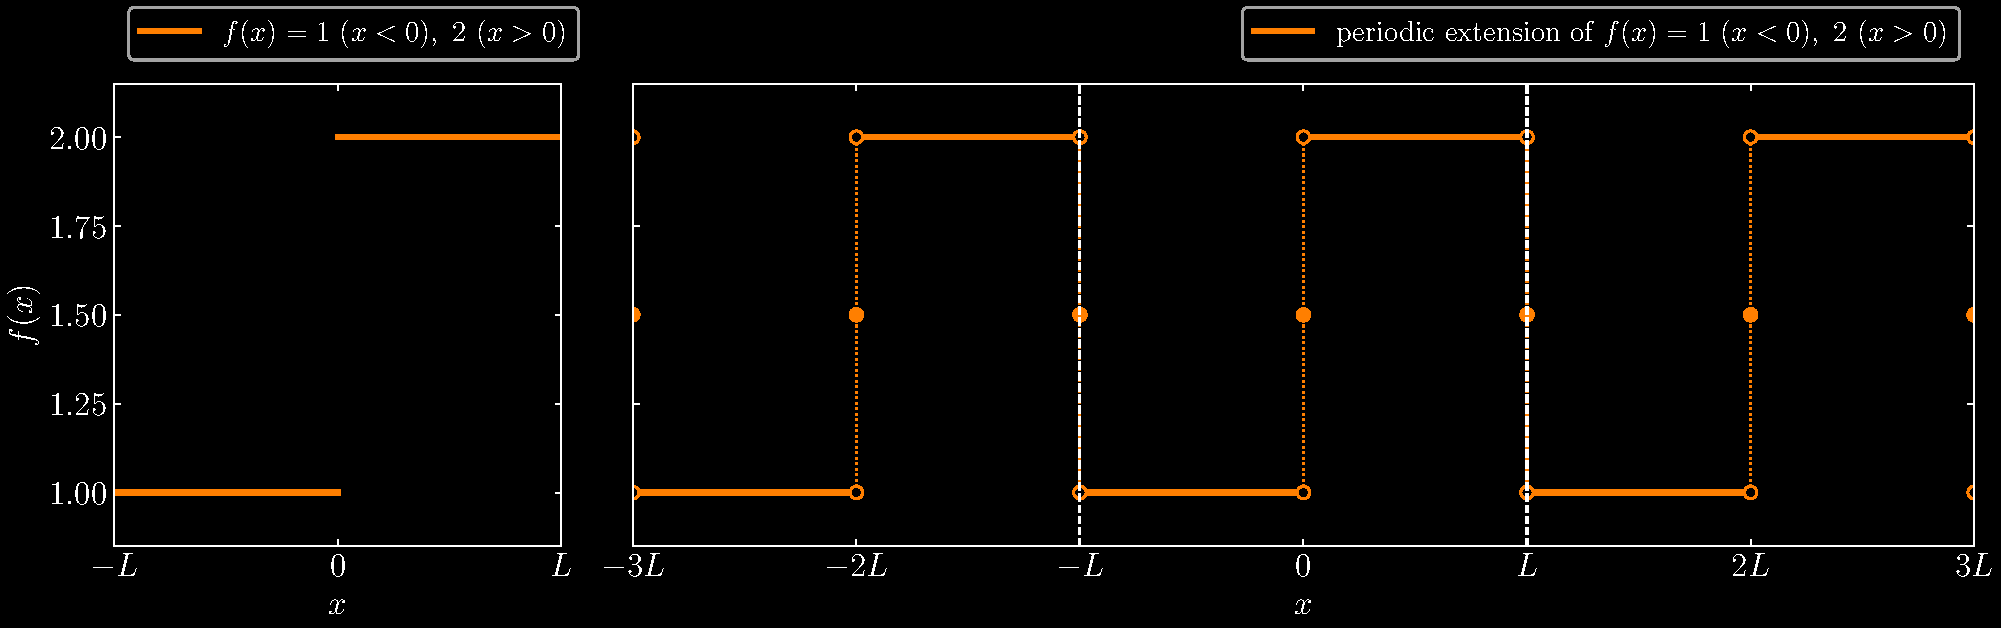
\includegraphics[width=0.9\textwidth]{../chap3/sec3.2/chap3sec3.2ex2g.pdf}
	\end{center}
\end{enumerate}

\newpage
% QUESTION 3
\qs{3.2.3}{Show that the Fourier series operation is linear: that is, show that the Fourier series of \( c_{1}f \!\left( x \right) + c_{2}g \!\left( x \right) \) is the sum of \( c_{1} \) times the Fourier series of \( f \!\left( x \right) \) and \( c_{2} \) times the Fourier series of \( g \!\left( x \right) \).}

Suppose that \( f \) and \( g \) have Fourier series defined over \( \!\left[ -L,L \right] \) with period \( 2L \). The respective coefficients for any function \( h \!\left( x \right) \) on the aforementioned interval are defined by
\begin{align*}
	\!\left[ a_{0} \right]_{h} & = \frac{1}{2L}\int^{L}_{-L} h \!\left( x \right) \, dx \\
	\!\left[ a_{n} \right]_{h} & = \frac{1}{L}\int^{L}_{-L} h \!\left( x \right)\cos\!\left(\frac{n \pi x}{L}\right) \, dx \\
	\!\left[ b_{n} \right]_{h} & = \frac{1}{L}\int^{L}_{-L} h \!\left( x \right)\sin\!\left(\frac{n \pi x}{L}\right) \, dx
\end{align*}
By linearity of integration, the coefficients for the linear combination are
\begin{align*}
	\!\left[ a_{n} \right]_{c_{1}f + c_{2}g} = \frac{1}{L}\int^{L}_{-L} \!\left[ c_{1}f \!\left( x \right) + c_{2}g \!\left( x \right) \right]\cos\!\left(\frac{n \pi x}{L}\right) \, dx & = c_{1}\!\left[ a_{n} \right]_{f} + c_{2}\!\left[ a_{n} \right]_{g} \\
	\!\left[ b_{n} \right]_{c_{1}f + c_{2}g} = \frac{1}{L}\int^{L}_{-L} \!\left[ c_{1}f \!\left( x \right) + c_{2}g \!\left( x \right) \right]\sin\!\left(\frac{n \pi x}{L}\right) \, dx & = c_{1}\!\left[ b_{n} \right]_{f} + c_{2}\!\left[ b_{n} \right]_{g}
\end{align*}
with an analogous calculation for \( \!\left[ a_{0} \right]_{h} \). Since the coefficients of the linear combination are the sum of \( c_{1} \) times the Fourier coefficients of \( f \) and \( c_{2} \) times the Fourier coefficients of \( g \), it follows that the Fourier series itself is composed of \( c_{1} \) times that of \( f \) plus \( c_{2} \) times that of \( g \), establishing that the Fourier series operation is linear.

\vspace{12pt}

% QUESTION 4
\qs{3.2.4}{Suppose that \( f \!\left( x \right) \) is piecewise smooth. What value does the Fourier series of \( f \!\left( x \right) \) converge to at the endpoint \( x = -L \)? at \( x = L \)?}

One subtlety to be mindful of is \( f \!\left( x \right) \) is defined over \( \!\left[ -L,L \right] \). Let the superscript \( + \) and \( - \) in \( f \!\left( x^{+} \right) \) and \( f \!\left( x^{-} \right) \) be defined as approaching \( x \) from above (the right) and below (the left). From the construction of our interval, however, it is impossible to have either \( f \!\left( -L^{-} \right) \) or \( f \!\left( L^{+} \right) \), for \( L \) and \( -L \) are the absolute maximum and minimum values of the interval. 

Fortunately, there is a workaround. Let \( F \) be the periodic extension of \( f \). Note that there is a difference in where \( F \) and \( f \) are defined; the former is over all \( x \), and the latter only on \( \!\left[ -L,L \right] \). By Fourier's theorem, the Fourier series of \( f \) converges to \( \frac{1}{2}\!\left[ F \!\left( x^{+} \right) + F \!\left( x^{-} \right) \right] \); by periodicity, this means that approaching the left boundary from below is akin to approaching the right boundary from below (and vice-versa for the other boundary). Equivalently,
\[
	F \!\left( -L^{-} \right) = f \!\left( L^{-} \right) \quad \text{and} \quad F \!\left( L^{+} \right) = f \!\left( -L^{+} \right)
\]
From this logic, it turns out that the point of convergence is the same at \( x = -L \) and \( x = L \), which is
\[
	\frac{1}{2}\!\left[ f \!\left( -L^{+} \right) + f \!\left( L^{-} \right) \right] 
\]

\newpage
\subsection{\textsf{3.3 - Fourier Cosine and Sine Series}}

% QUESTION 1
\qs{3.3.1}{For the following functions, sketch \( f \!\left( x \right) \), the Fourier series of \( f \!\left( x \right) \), the Fourier sine series of \( f \!\left( x \right) \), and the Fourier cosine series of \( f \!\left( x \right) \).
\begin{enumerate}[label=(\alph*)]
	\item \( f \!\left( x \right) = 1 \)
	\item \( f \!\left( x \right) = 1 + x \)
	\item \( f \!\left( x \right) = \begin{cases}
		x & x < 0 \\
		1 + x & x > 0 
	\end{cases} \)
	\item \( f \!\left( x \right) = e^{x} \)
	\item \( f \!\left( x \right) = \begin{cases}
		2 & x < 0 \\
		e^{-x} & x > 0 
	\end{cases} \)
\end{enumerate}}

\begin{enumerate}[label=(\alph*)]
	\item 
	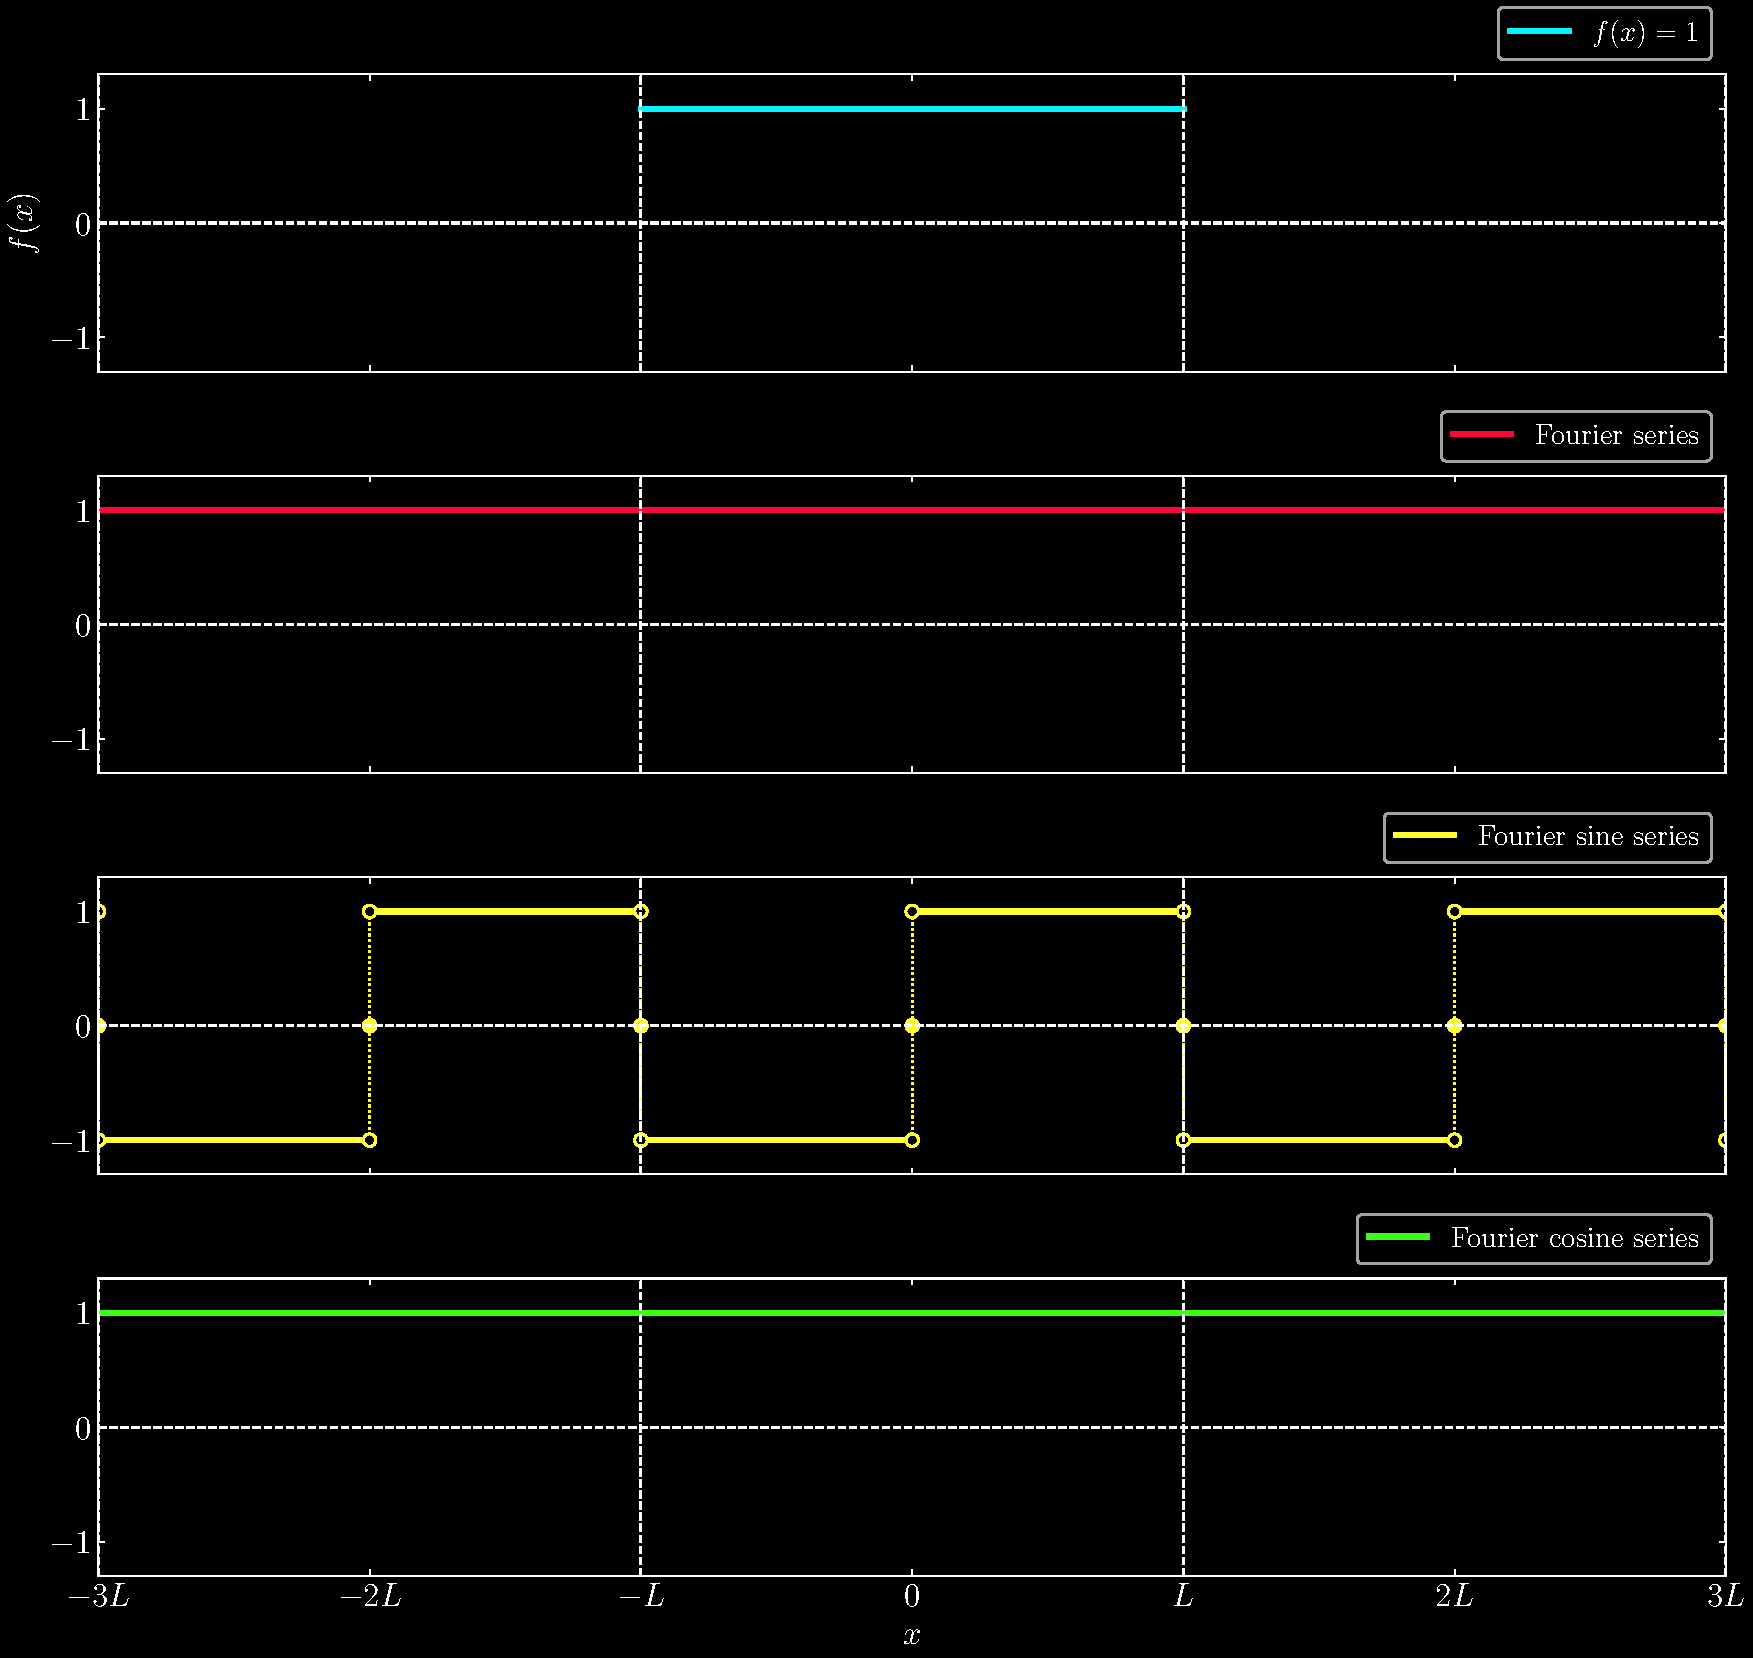
\includegraphics[width=0.9\textwidth]{../chap3/sec3.3/chap3sec3.3ex1a.pdf}
	\item 
	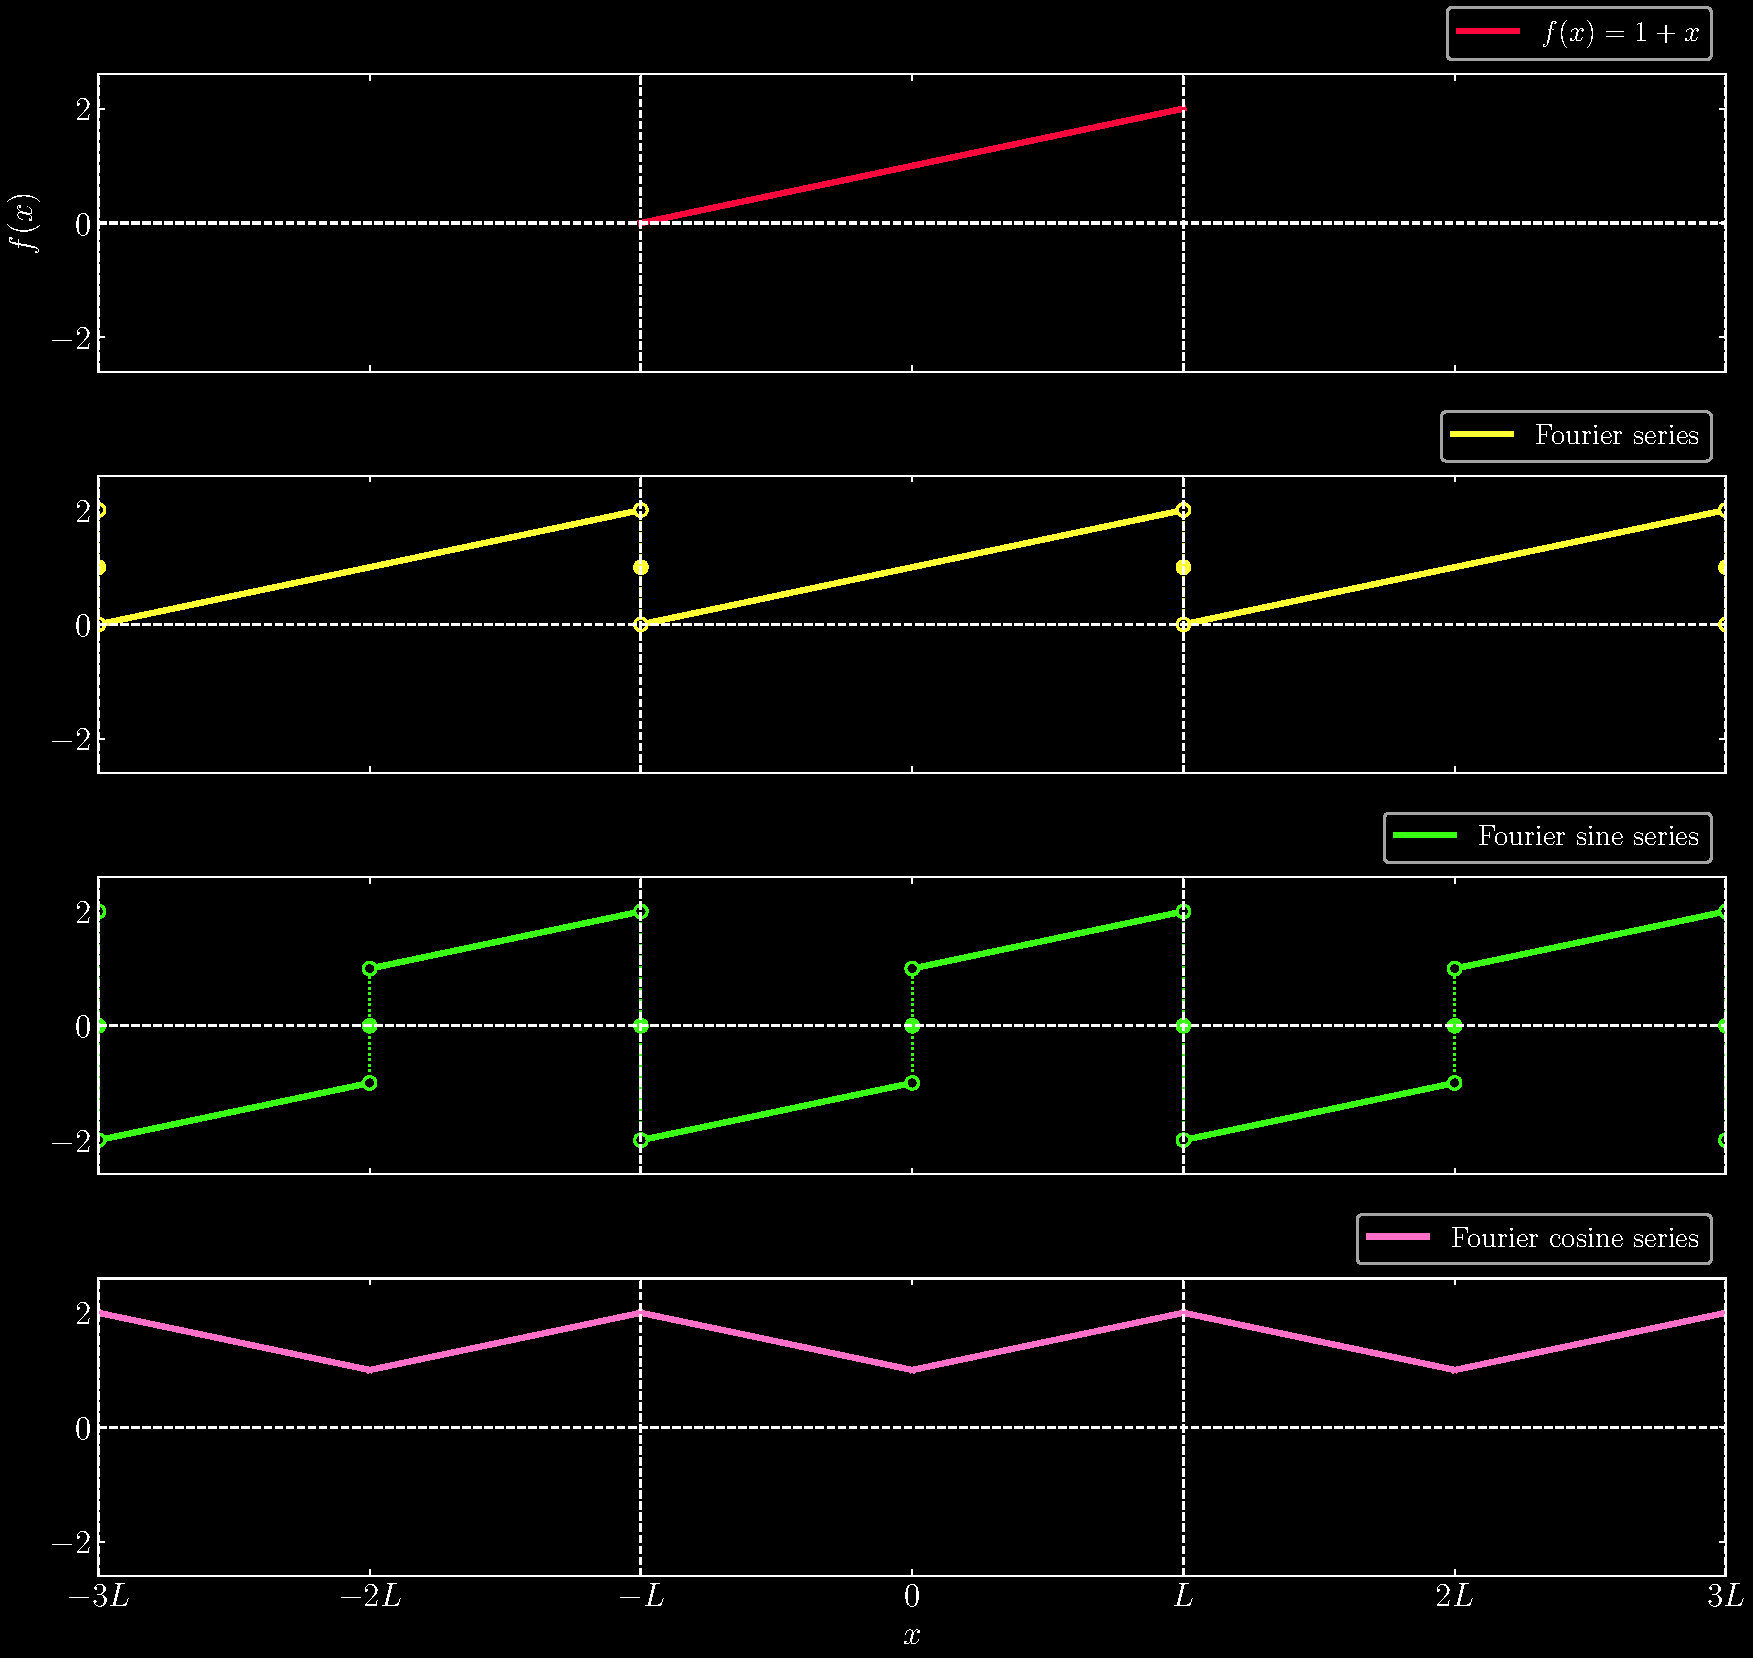
\includegraphics[width=0.9\textwidth]{../chap3/sec3.3/chap3sec3.3ex1b.pdf}
	\item 
	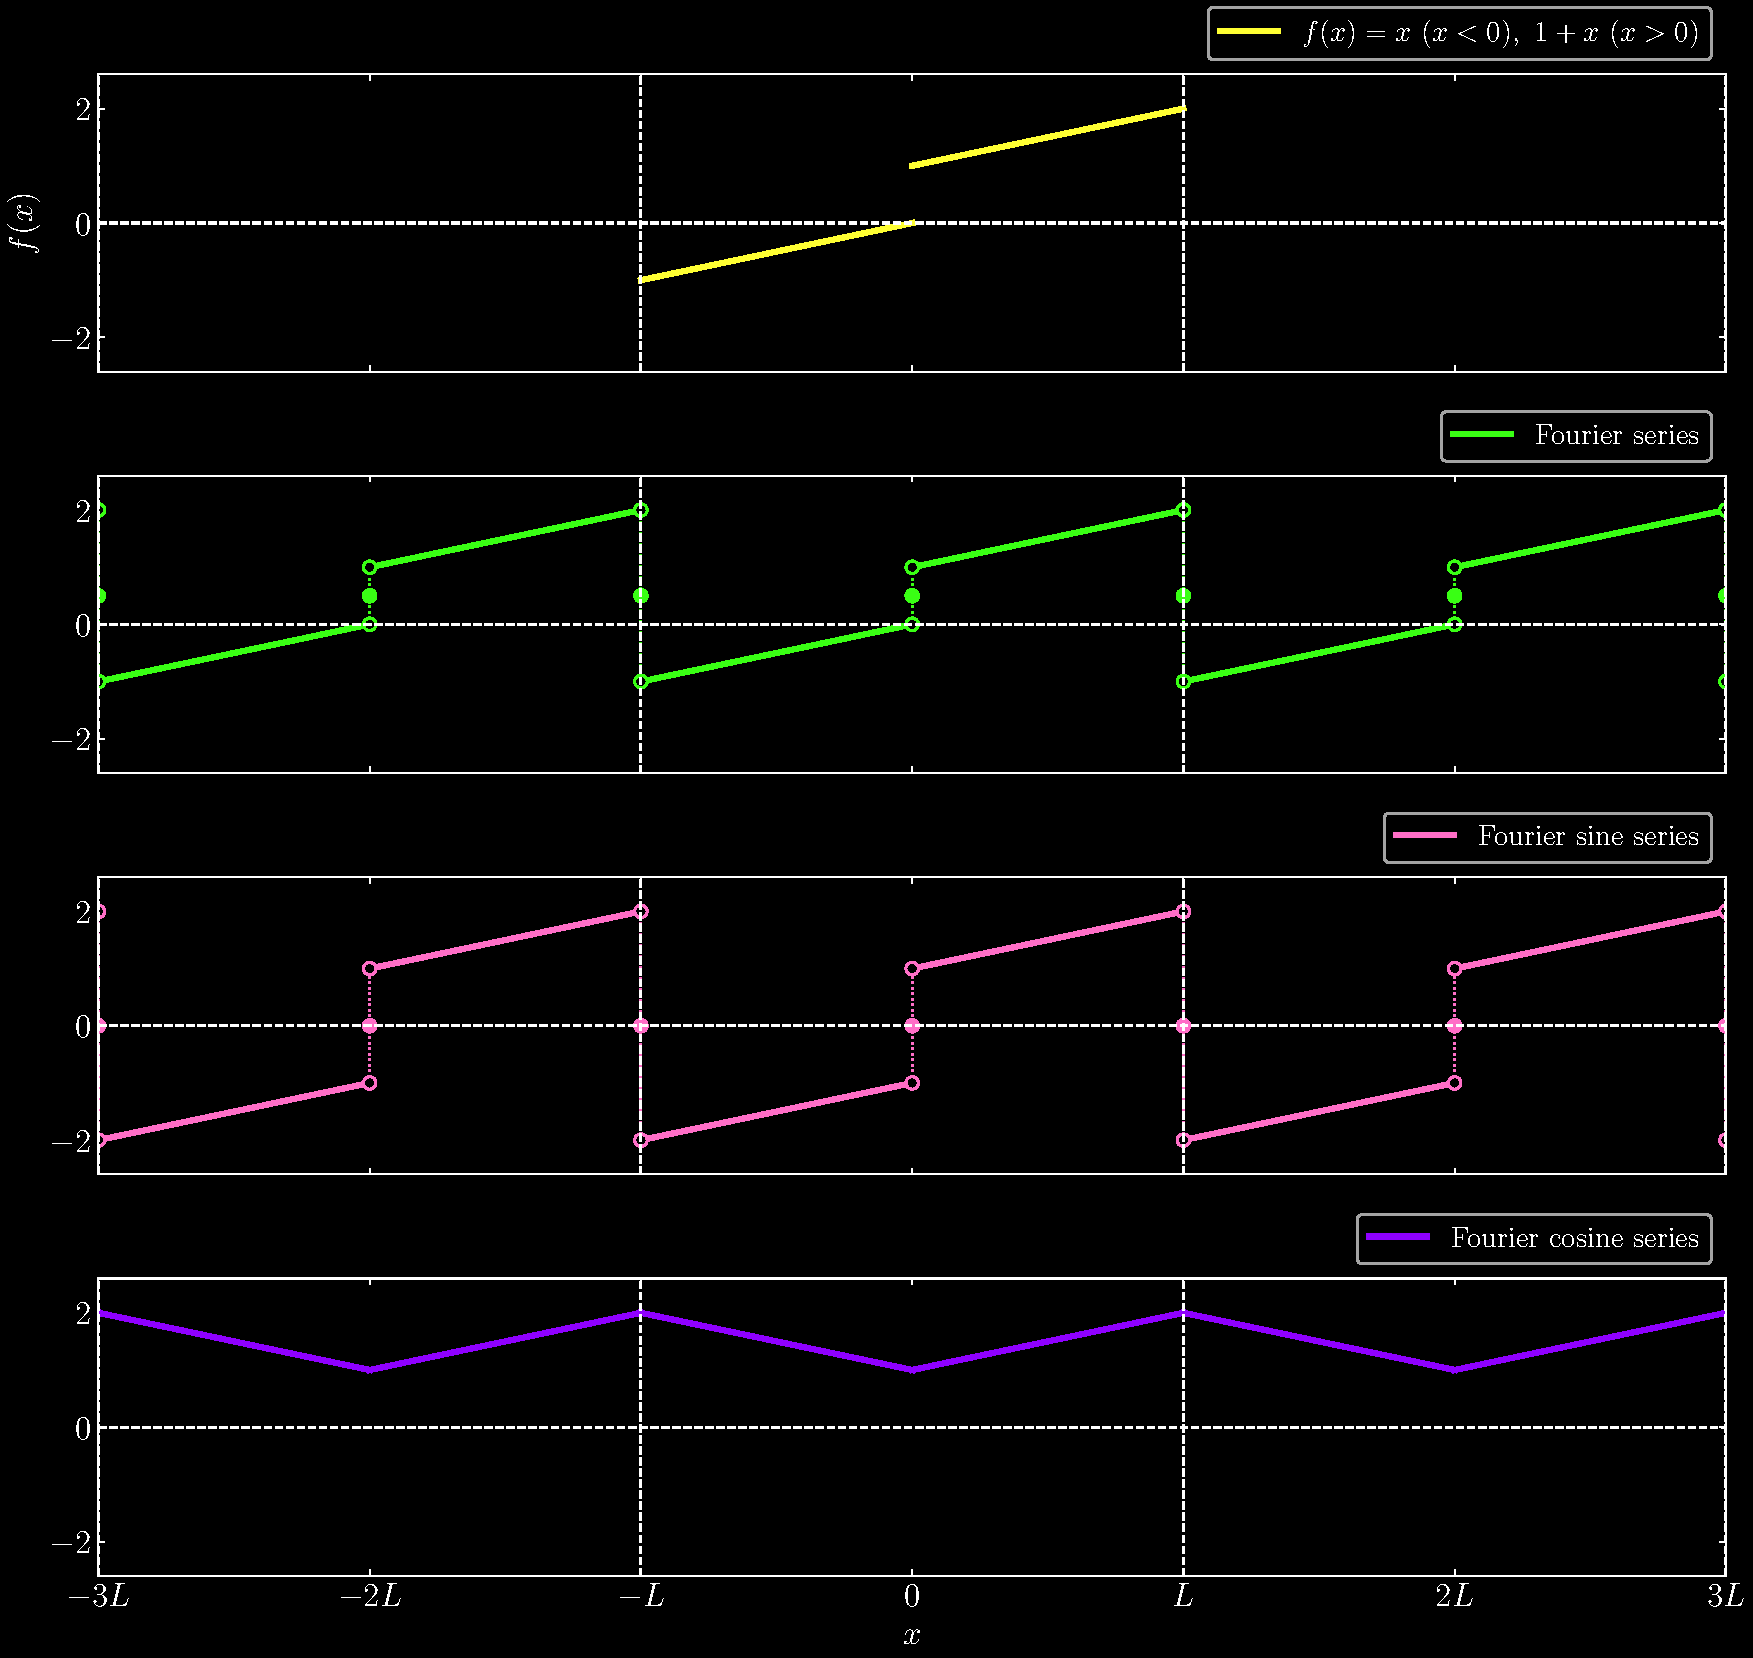
\includegraphics[width=0.9\textwidth]{../chap3/sec3.3/chap3sec3.3ex1c.pdf}
	\item 
	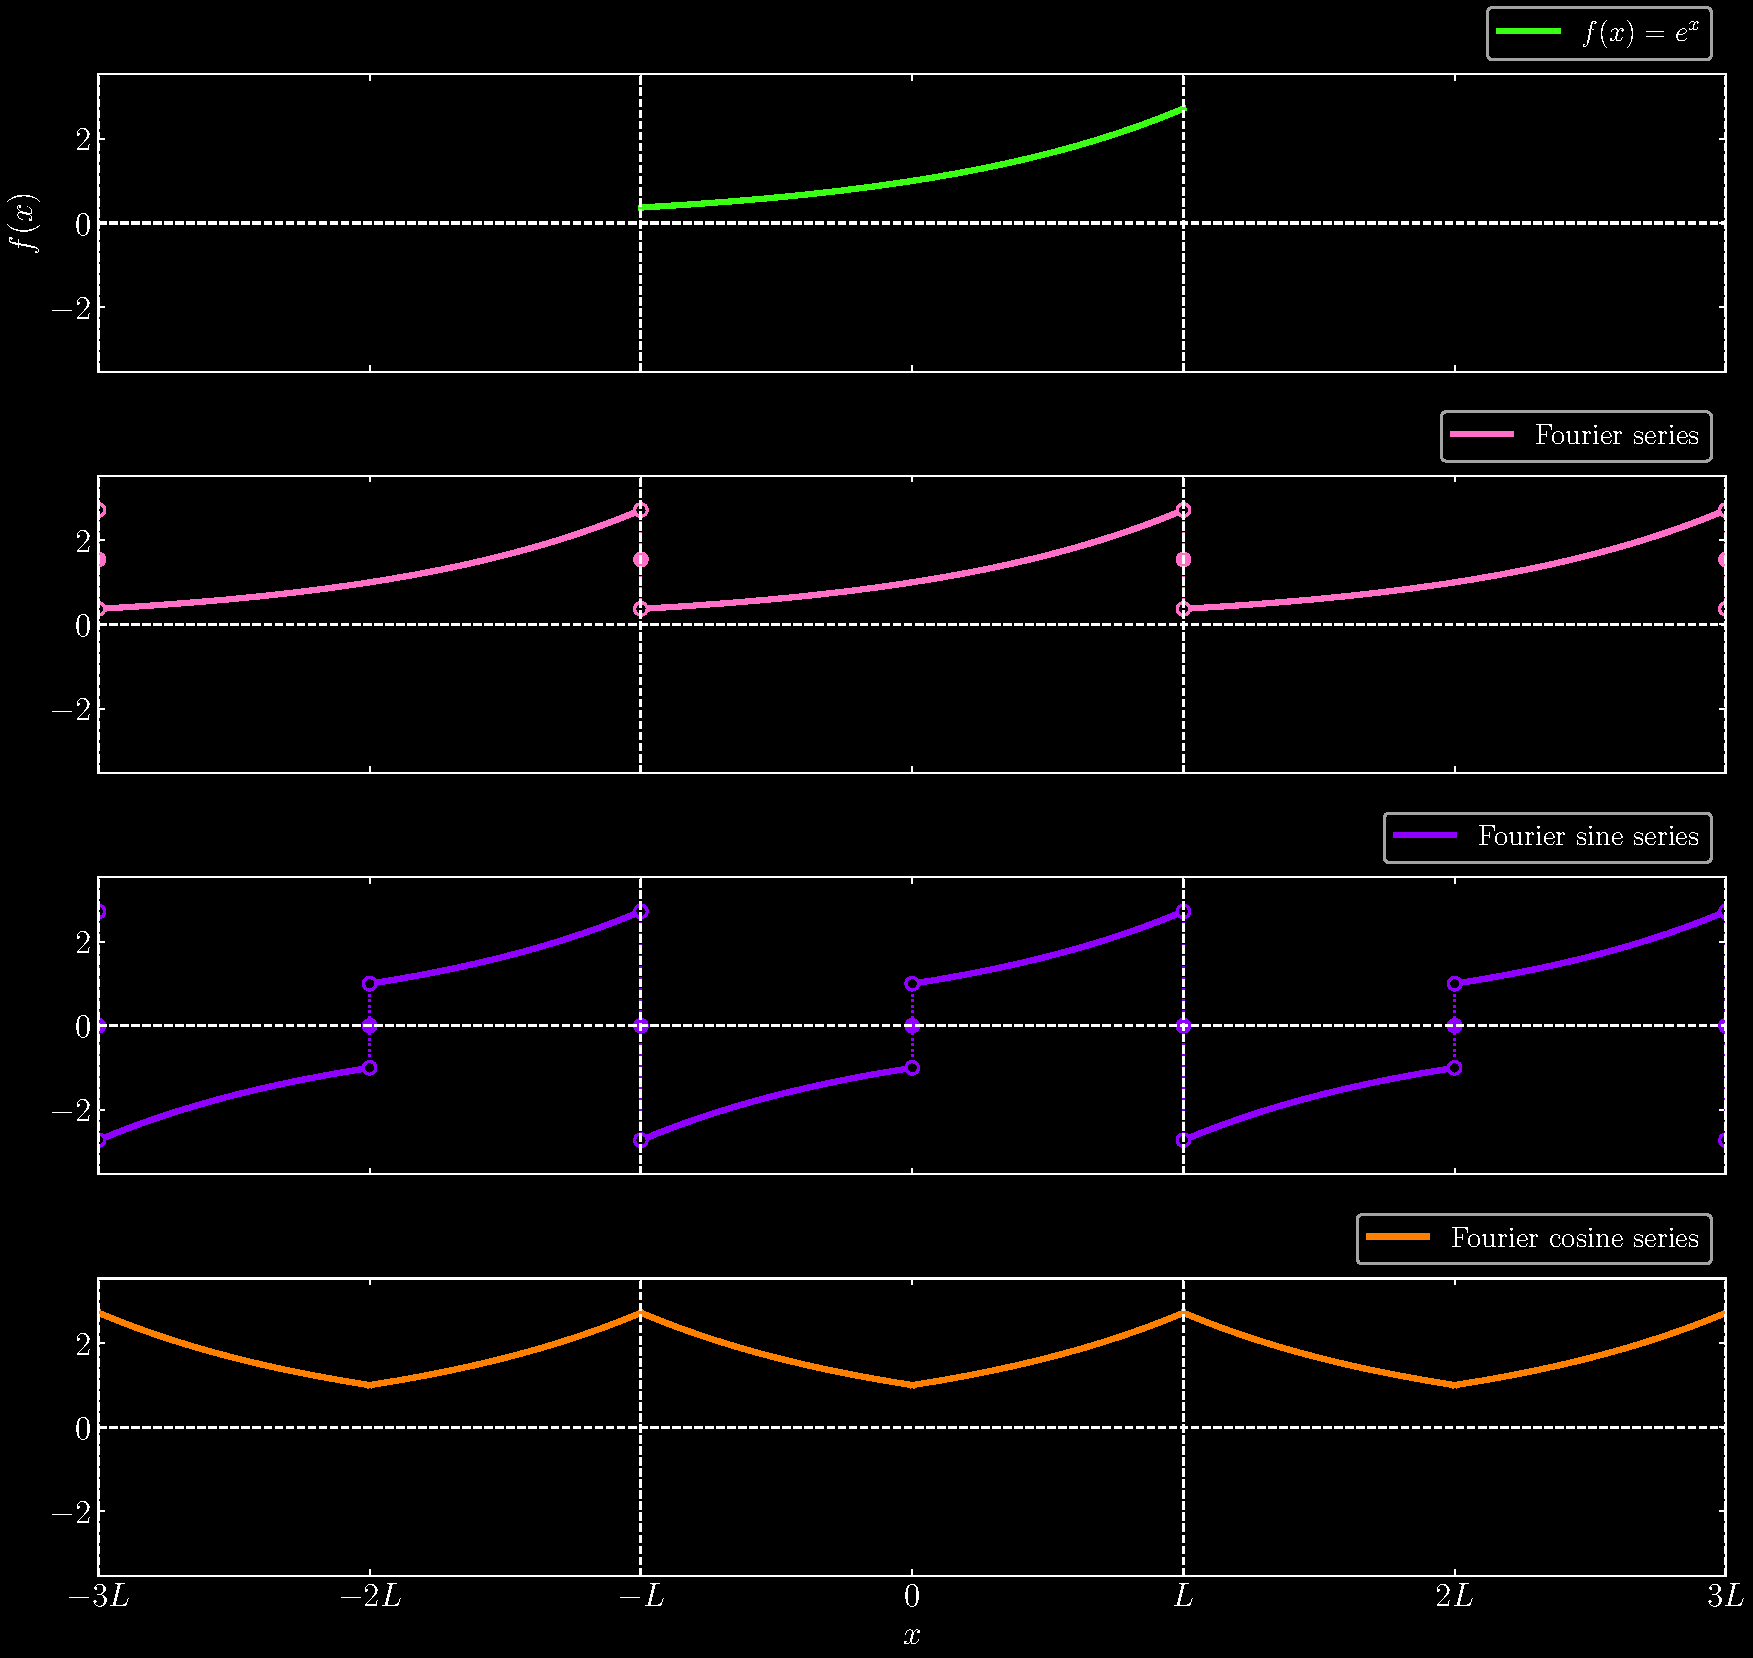
\includegraphics[width=0.9\textwidth]{../chap3/sec3.3/chap3sec3.3ex1d.pdf}
	\item 
	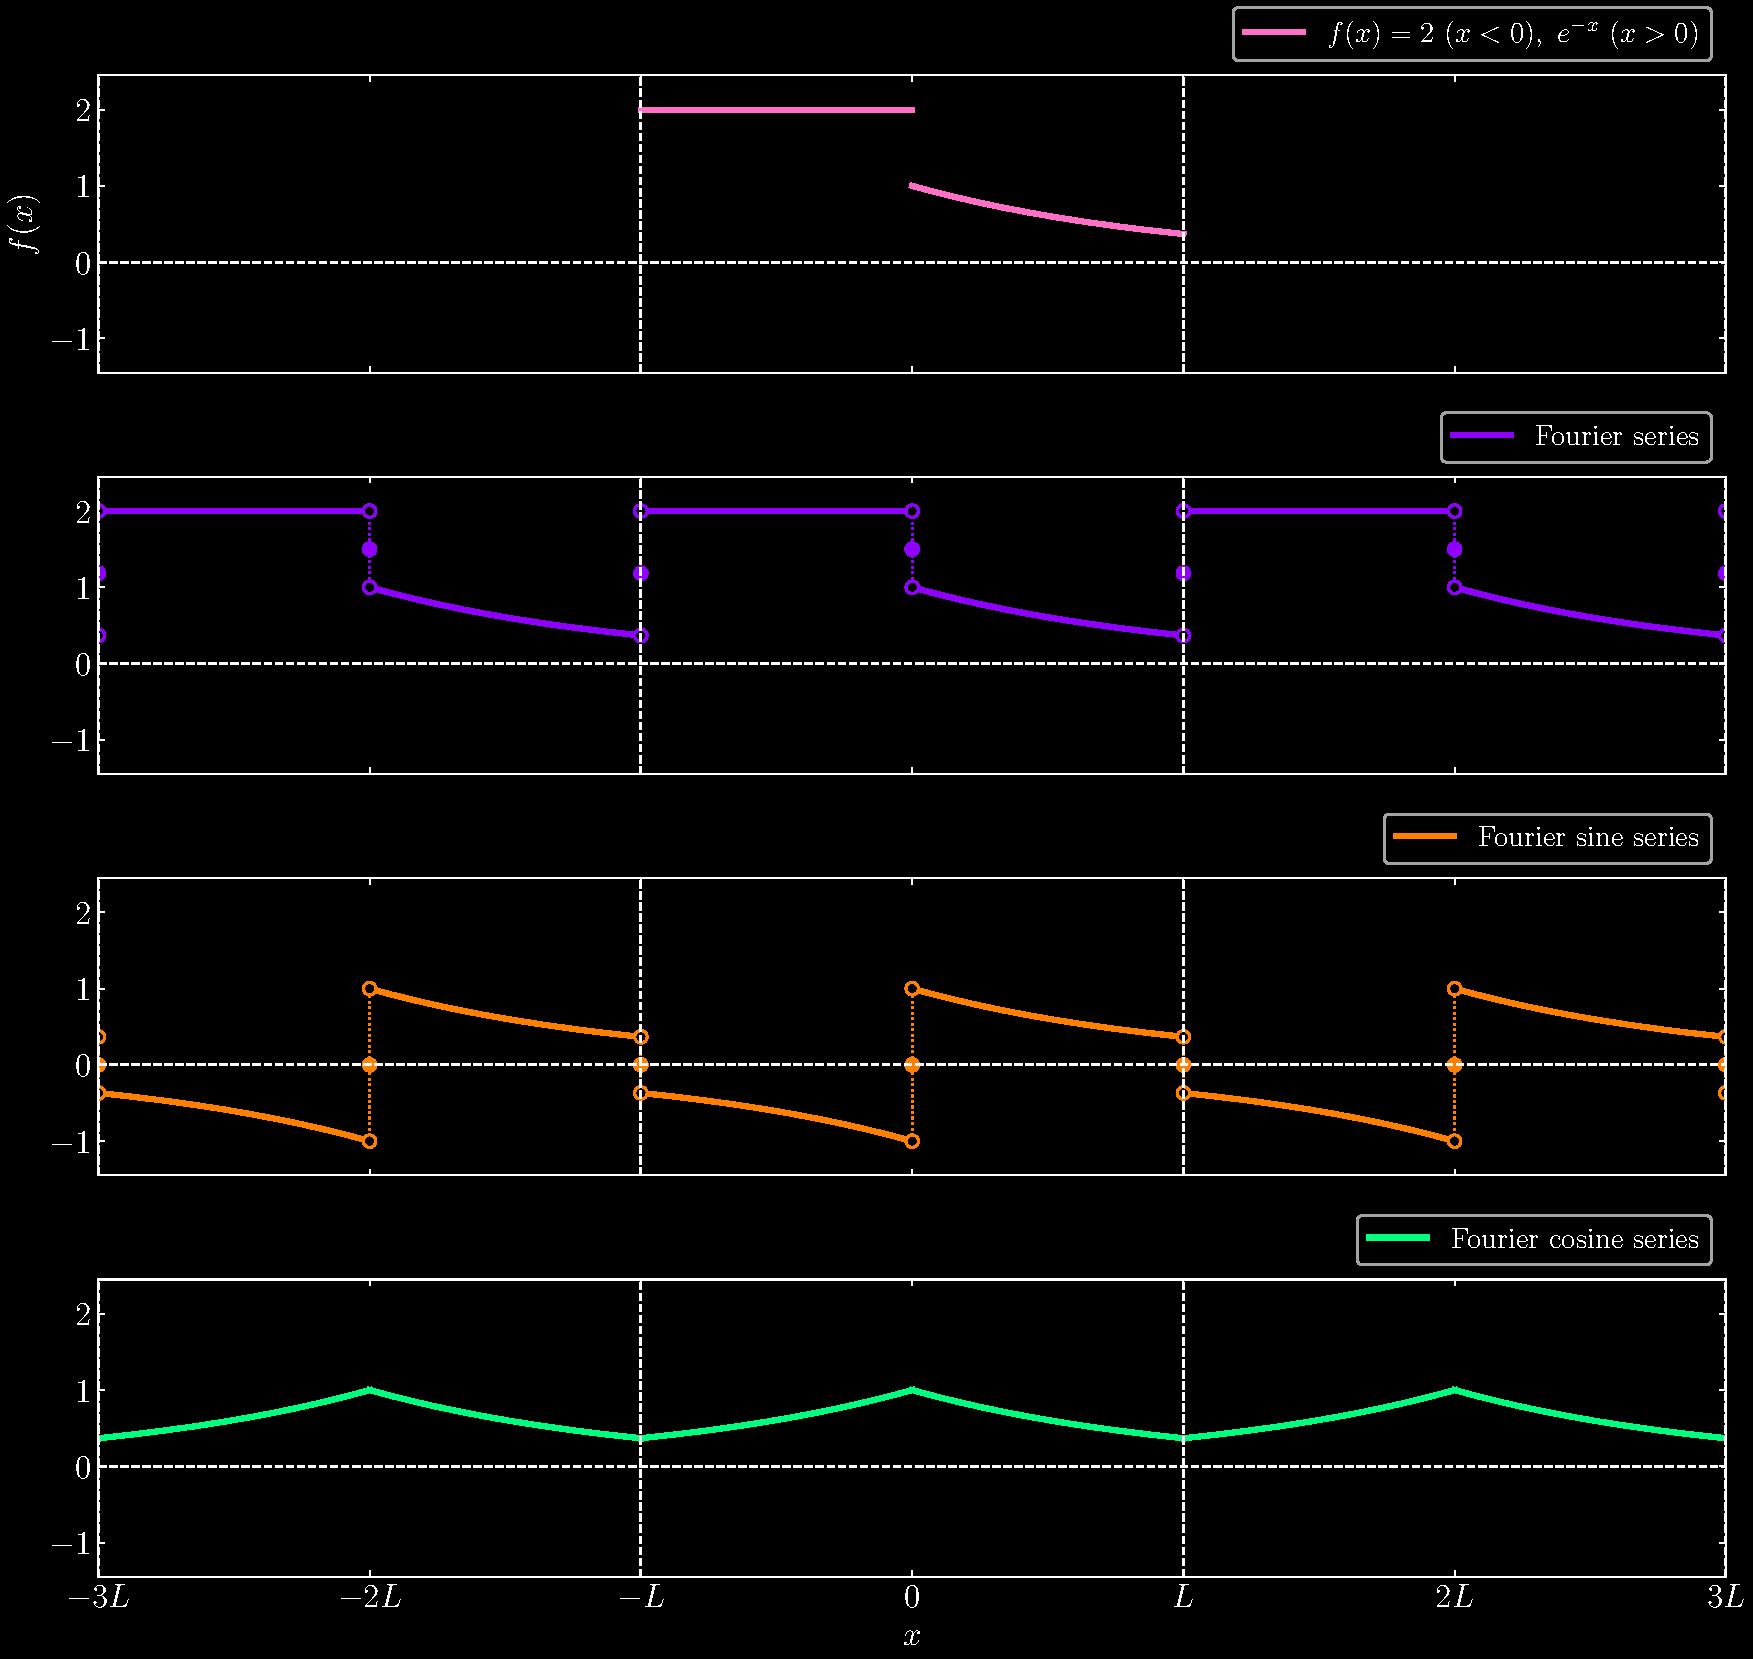
\includegraphics[width=0.9\textwidth]{../chap3/sec3.3/chap3sec3.3ex1e.pdf}
\end{enumerate}

% QUESTION 2
\qs{3.3.2}{For the following functions, sketch the Fourier sine series of \( f \!\left( x \right) \) and determine its Fourier coefficients:
\begin{enumerate}[label=(\alph*)]
	\item \( f \!\left( x \right) = \cos\!\left(\pi x / L\right) \) [Verify formula (3.3.13).]
	\item \( f \!\left( x \right) = \begin{cases}
		1 & x < L/6 \\
		3 & L/6 < x < L/2 \\
		0 & x > L/2
	\end{cases} \)
	\item \( f \!\left( x \right) = \begin{cases}
		0 & x < L/2 \\
		x & x > L/2 
	\end{cases} \)
	\item \( f \!\left( x \right) = \begin{cases}
		1 & x < L/2 \\
		0 & x > L/2 
	\end{cases} \)
\end{enumerate}}

\begin{enumerate}[label=(\alph*)]
	\item \begin{align*}
		B_{1} & = \frac{2}{L}\int^{L}_{0} \cos\!\left(\frac{\pi x}{L}\right)\sin\!\left(\frac{\pi x}{L}\right) \, dx \\
		      & = \frac{1}{L}\int^{L}_{0} \sin\!\left(\frac{2\pi x}{L}\right) \, dx \\
      & = -\frac{1}{2\pi}\cos\!\left(\frac{2\pi x}{L}\right)\Big|^{L}_{0} \\
      & = 0 \\
		B_{n} & = \frac{2}{L}\int^{L}_{0} \cos\!\left(\frac{\pi x}{L}\right)\sin\!\left(\frac{n \pi x}{L}\right) \, dx \\
		& = \frac{1}{L}\int^{L}_{0} \left[\sin\!\left(\frac{(n+1) \pi x}{L}\right) + \sin\!\left(\frac{(n-1) \pi x}{L}\right)\right] dx \\
      & = \frac{1}{\pi}\left(1 - (-1)^{n+1}\right)\left[\frac{1}{n+1} + \frac{1}{n-1}\right] \\
      & = \frac{2n\left(1 + (-1)^n\right)}{\pi\left(n^2 - 1\right)}, \qquad n \neq 1
	\end{align*}
	The \( B_{n} \) coefficients split into even and odd cases:
	\[
		B_{n} = \begin{cases}
			0 & n \text{ odd} \\
			\displaystyle{\frac{4n}{\pi \!\left( n^{2} - 1 \right)}} & n \text{ even} 
		\end{cases}
	\]
	verifying equation (3.3.13).

	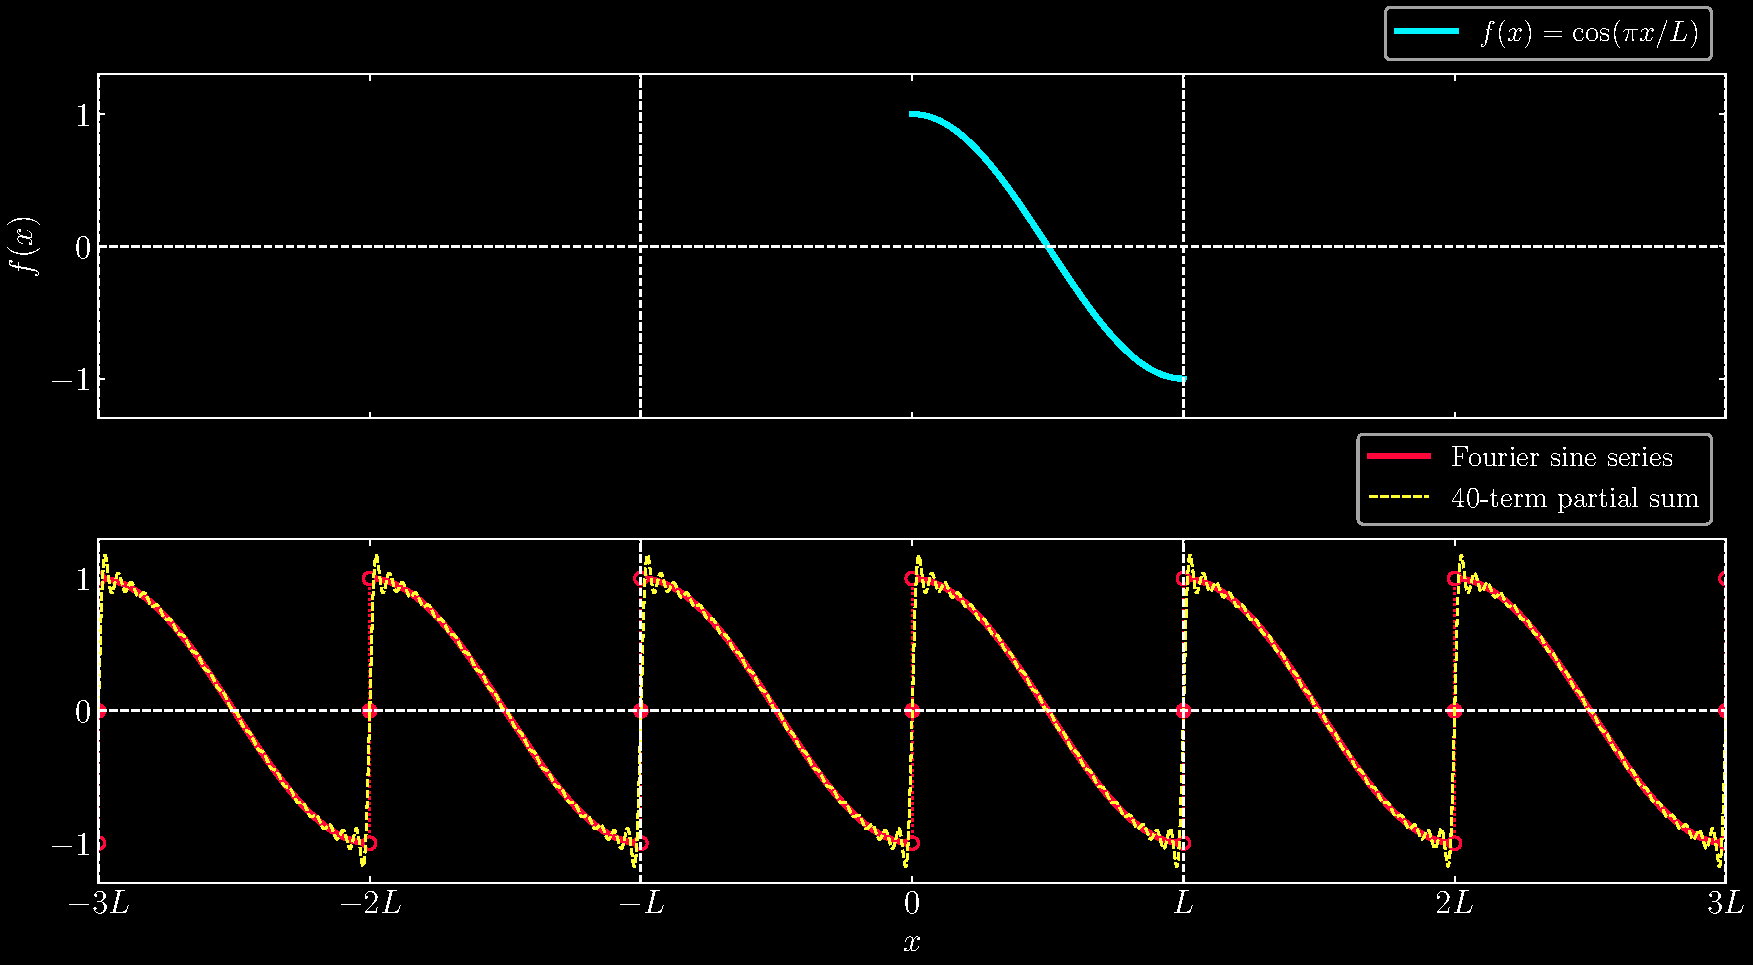
\includegraphics[width=0.9\textwidth]{../chap3/sec3.3/chap3sec3.3ex2a.pdf}
	\item \begin{align*}
			B_{n} & = \frac{2}{L}\!\left[ \int^{L/6}_{0} \sin\!\left(\frac{n \pi x}{L}\right) \, dx + 3\int^{L/2}_{L/6} \sin\!\left(\frac{n \pi x}{L}\right) \, dx \right] \\
			      & = \frac{2}{L}\cdot\frac{L}{n\pi}\left[ -\cos\!\left(\frac{n \pi x}{L}\right)\Big|^{L/6}_{0} - 3\cos\!\left(\frac{n \pi x}{L}\right)\Big|^{L/2}_{L/6} \right] \\
      & = \frac{2}{n\pi}\left[ \left(1 - \cos\!\left(\frac{n\pi}{6}\right)\right) + 3\left(\cos\!\left(\frac{n\pi}{6}\right) - \cos\!\left(\frac{n\pi}{2}\right)\right) \right] \\
      & = \frac{2}{n\pi}\left[ 1 + 2\cos\!\left(\frac{n\pi}{6}\right) - 3\cos\!\left(\frac{n\pi}{2}\right) \right]
	\end{align*}
	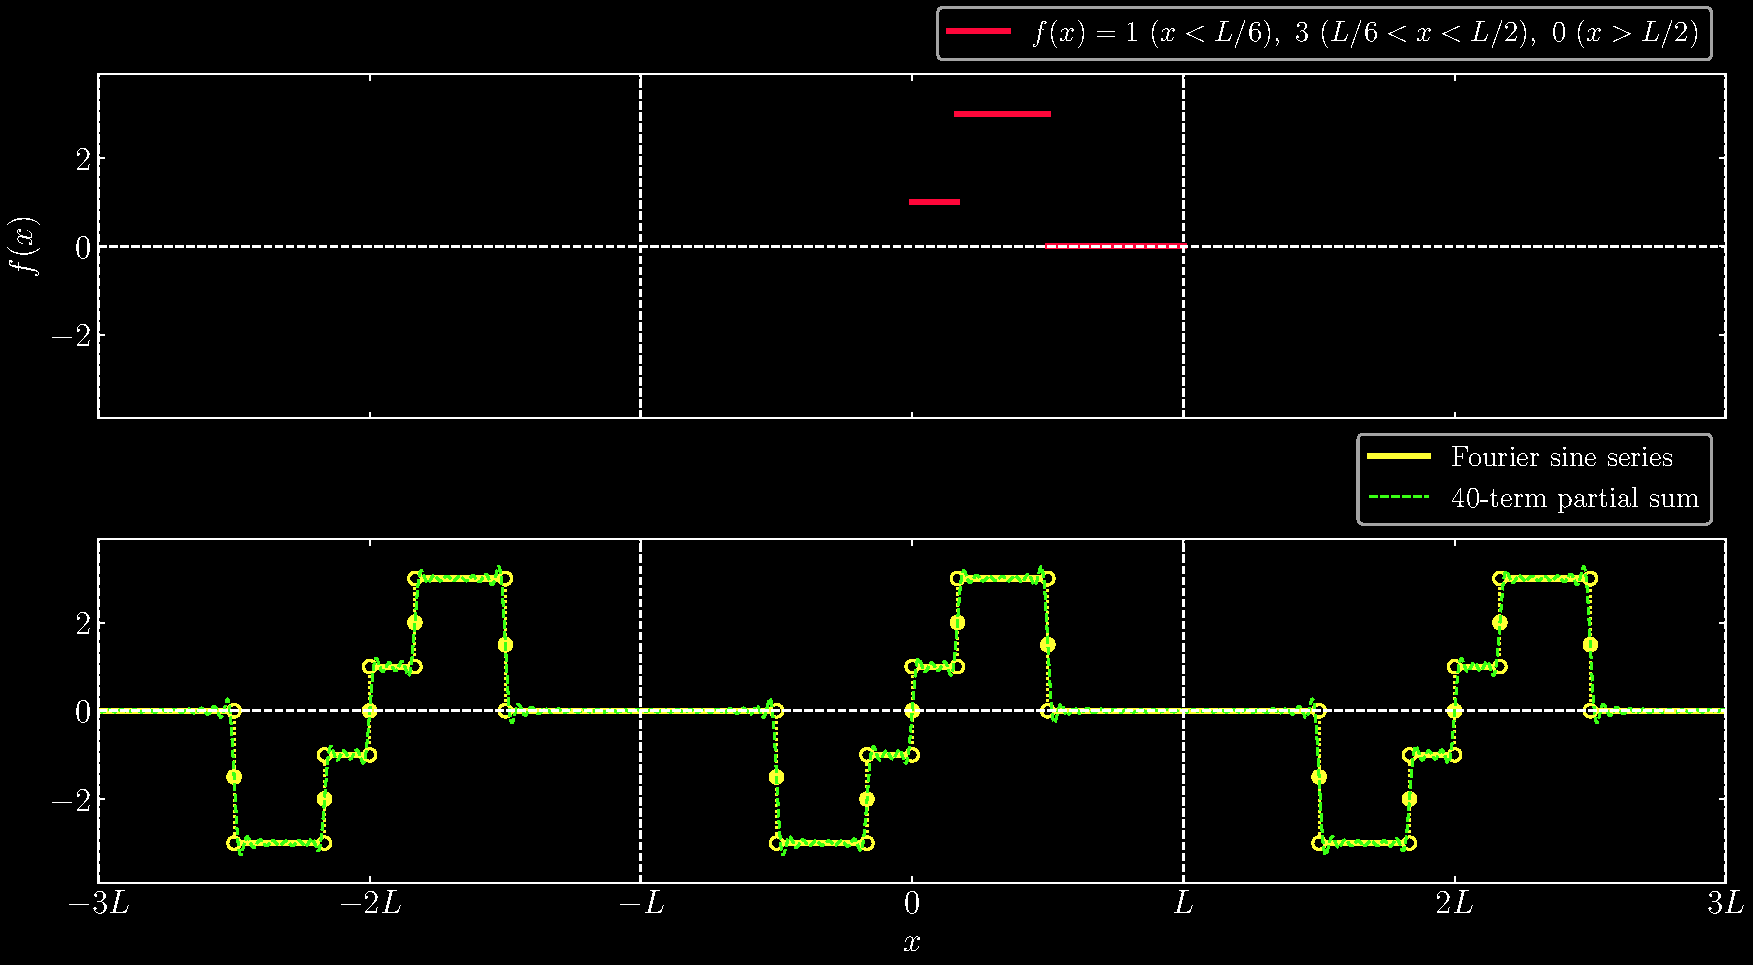
\includegraphics[width=0.9\textwidth]{../chap3/sec3.3/chap3sec3.3ex2b.pdf}
	\item \begin{align*}
		B_{n} & = \frac{2}{L}\int^{L}_{L/2} x \sin\!\left(\frac{n \pi x}{L}\right) \, dx \\
		& = \frac{2}{L}\left[ -\frac{L}{n\pi}\,x\cos\!\left(\frac{n \pi x}{L}\right)\Big|^{L}_{L/2} + \frac{L}{n\pi}\int^{L}_{L/2} \cos\!\left(\frac{n \pi x}{L}\right) \, dx \right] \\
      & = \frac{2}{L}\left[ -\frac{L}{n\pi}\left( L(-1)^n - \frac{L}{2}\cos\!\left(\frac{n\pi}{2}\right) \right) + \frac{L^2}{n^2\pi^2}\sin\!\left(\frac{n \pi x}{L}\right)\Big|^{L}_{L/2} \right] \\
      & = \frac{2L}{n\pi}\left[ \frac{1}{2}\cos\!\left(\frac{n\pi}{2}\right) - (-1)^n \right] - \frac{2L}{n^2\pi^2}\sin\!\left(\frac{n\pi}{2}\right)
	\end{align*}
	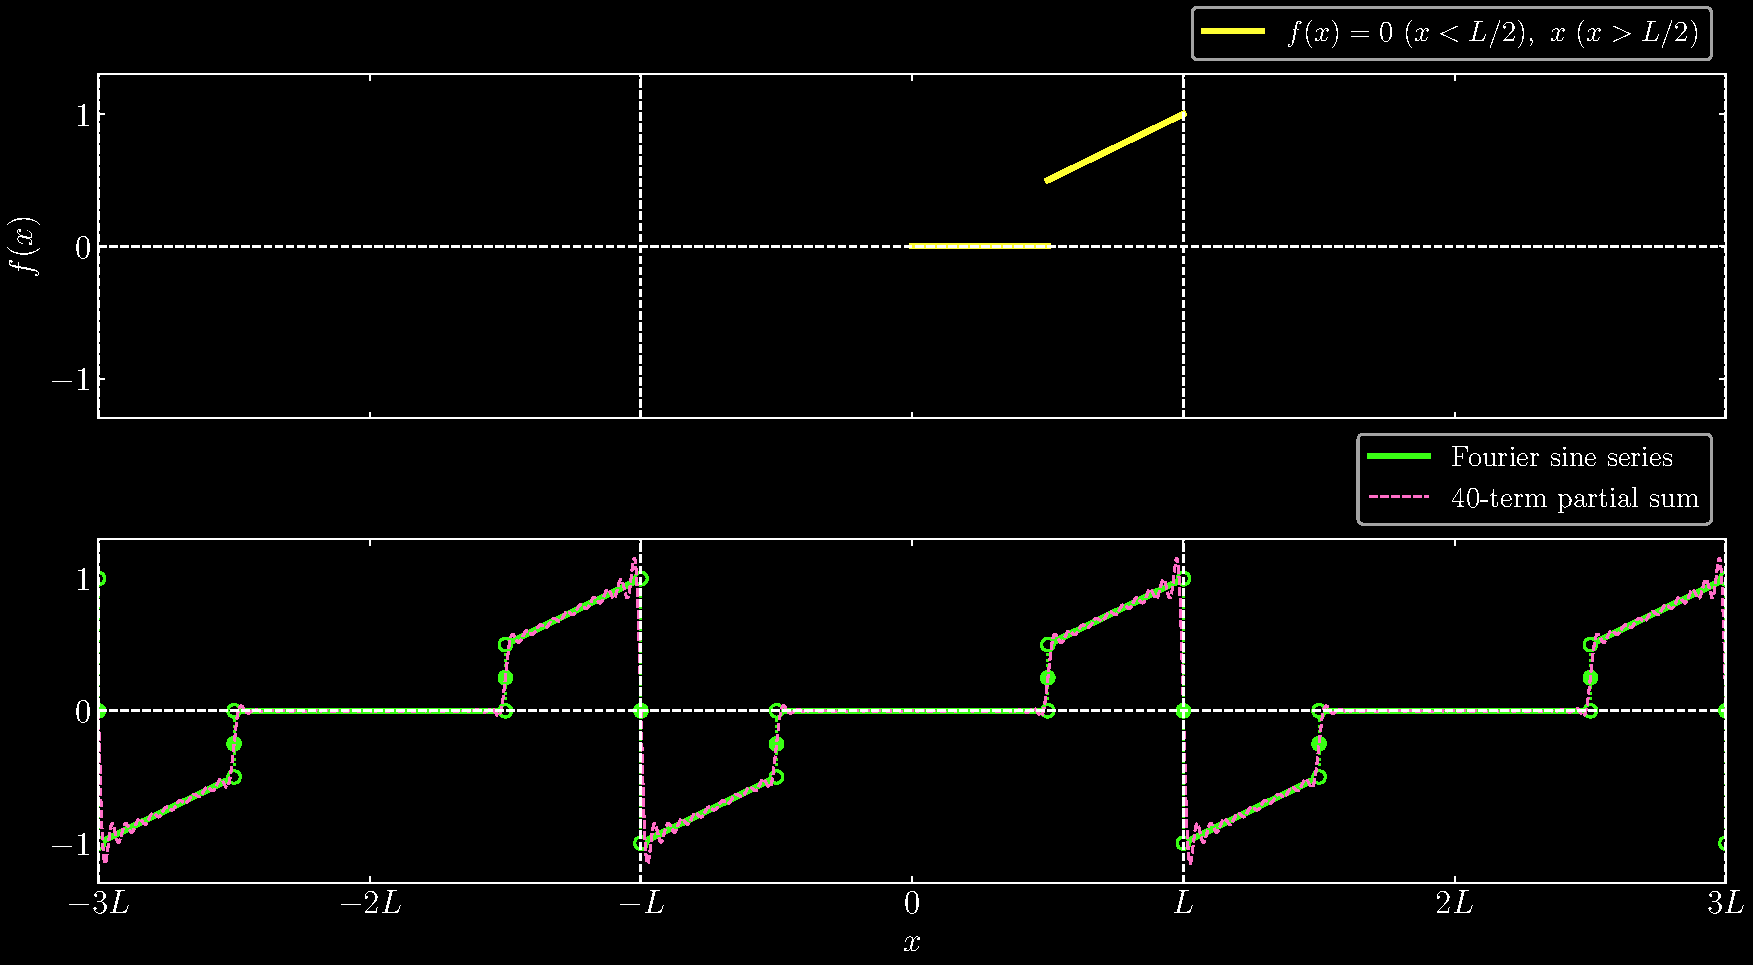
\includegraphics[width=0.9\textwidth]{../chap3/sec3.3/chap3sec3.3ex2c.pdf}
	\item \begin{align*}
		B_{n} & = \frac{2}{L}\int^{L/2}_{0} \sin\!\left(\frac{n \pi x}{L}\right) \, dx \\
		 & = -\frac{2}{n \pi}\cos\!\left(\frac{n \pi x}{L}\right)\Big|^{L/2}_{0} \\ 
		 & = \frac{2}{n \pi}\!\left[ 1 - \cos\!\left(\frac{n \pi}{2}\right) \right] \\
		 & = \begin{cases}
			 \displaystyle{\frac{2}{n \pi}} & n \text{ odd} \\[10pt]
			\displaystyle{\frac{1}{m \pi}\!\left( 1 - \!\left( -1 \right)^{m} \right)} & n = 2m 
		 \end{cases}
	\end{align*}
	where we substitute \( n = 2m \). 
	\vspace{6pt}

	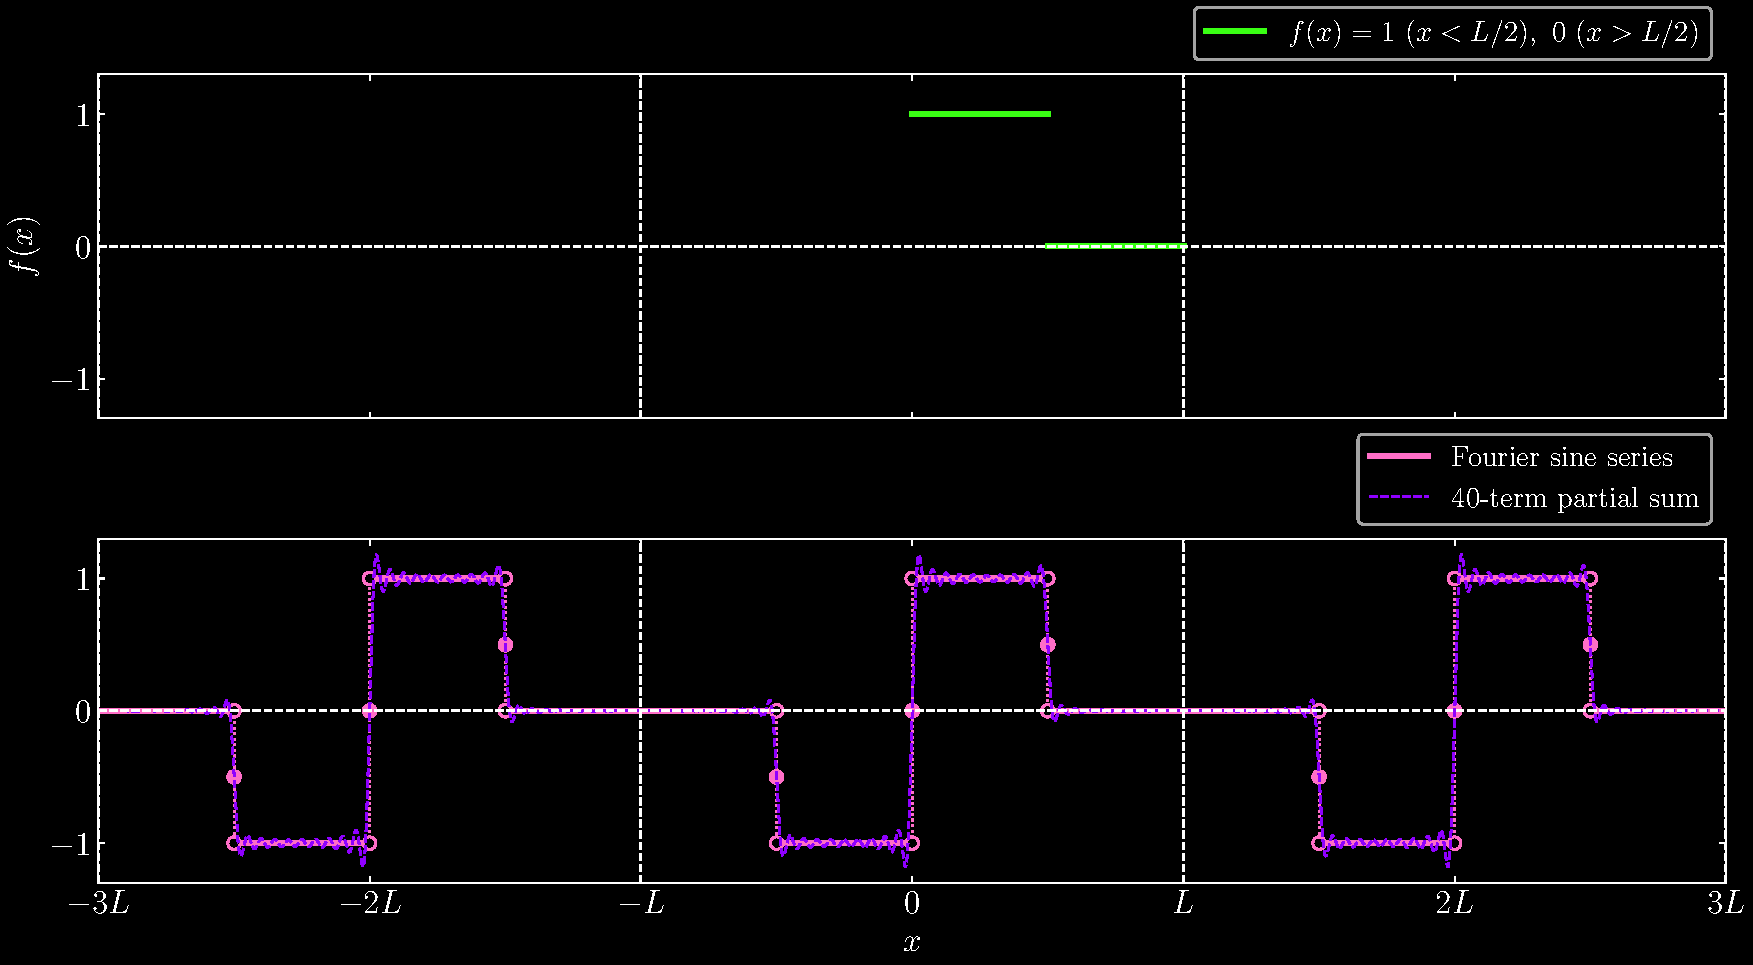
\includegraphics[width=0.9\textwidth]{../chap3/sec3.3/chap3sec3.3ex2d.pdf}
\end{enumerate}

\newpage
% QUESTION 3
\qs{3.3.3}{For the following functions, sketch the Fourier sine series of \( f \!\left( x \right) \). Also, roughly sketch the sum of a \textit{finite} number of nonzero terms (at least the first two) of the Fourier sine series:
\begin{enumerate}[label=(\alph*)]
	\item \( f \!\left( x \right) = \cos\!\left(\pi x / L\right) \) [Use formula (3.3.13).]
	\item \( f \!\left( x \right) = \begin{cases}
		1 & x < L/2 \\
		0 & x > L/2 
	\end{cases} \)
\item \( f \!\left( x \right) = x \) [Use formula (3.3.12).]
\end{enumerate}}

\begin{enumerate}[label=(\alph*)]
	\item 
	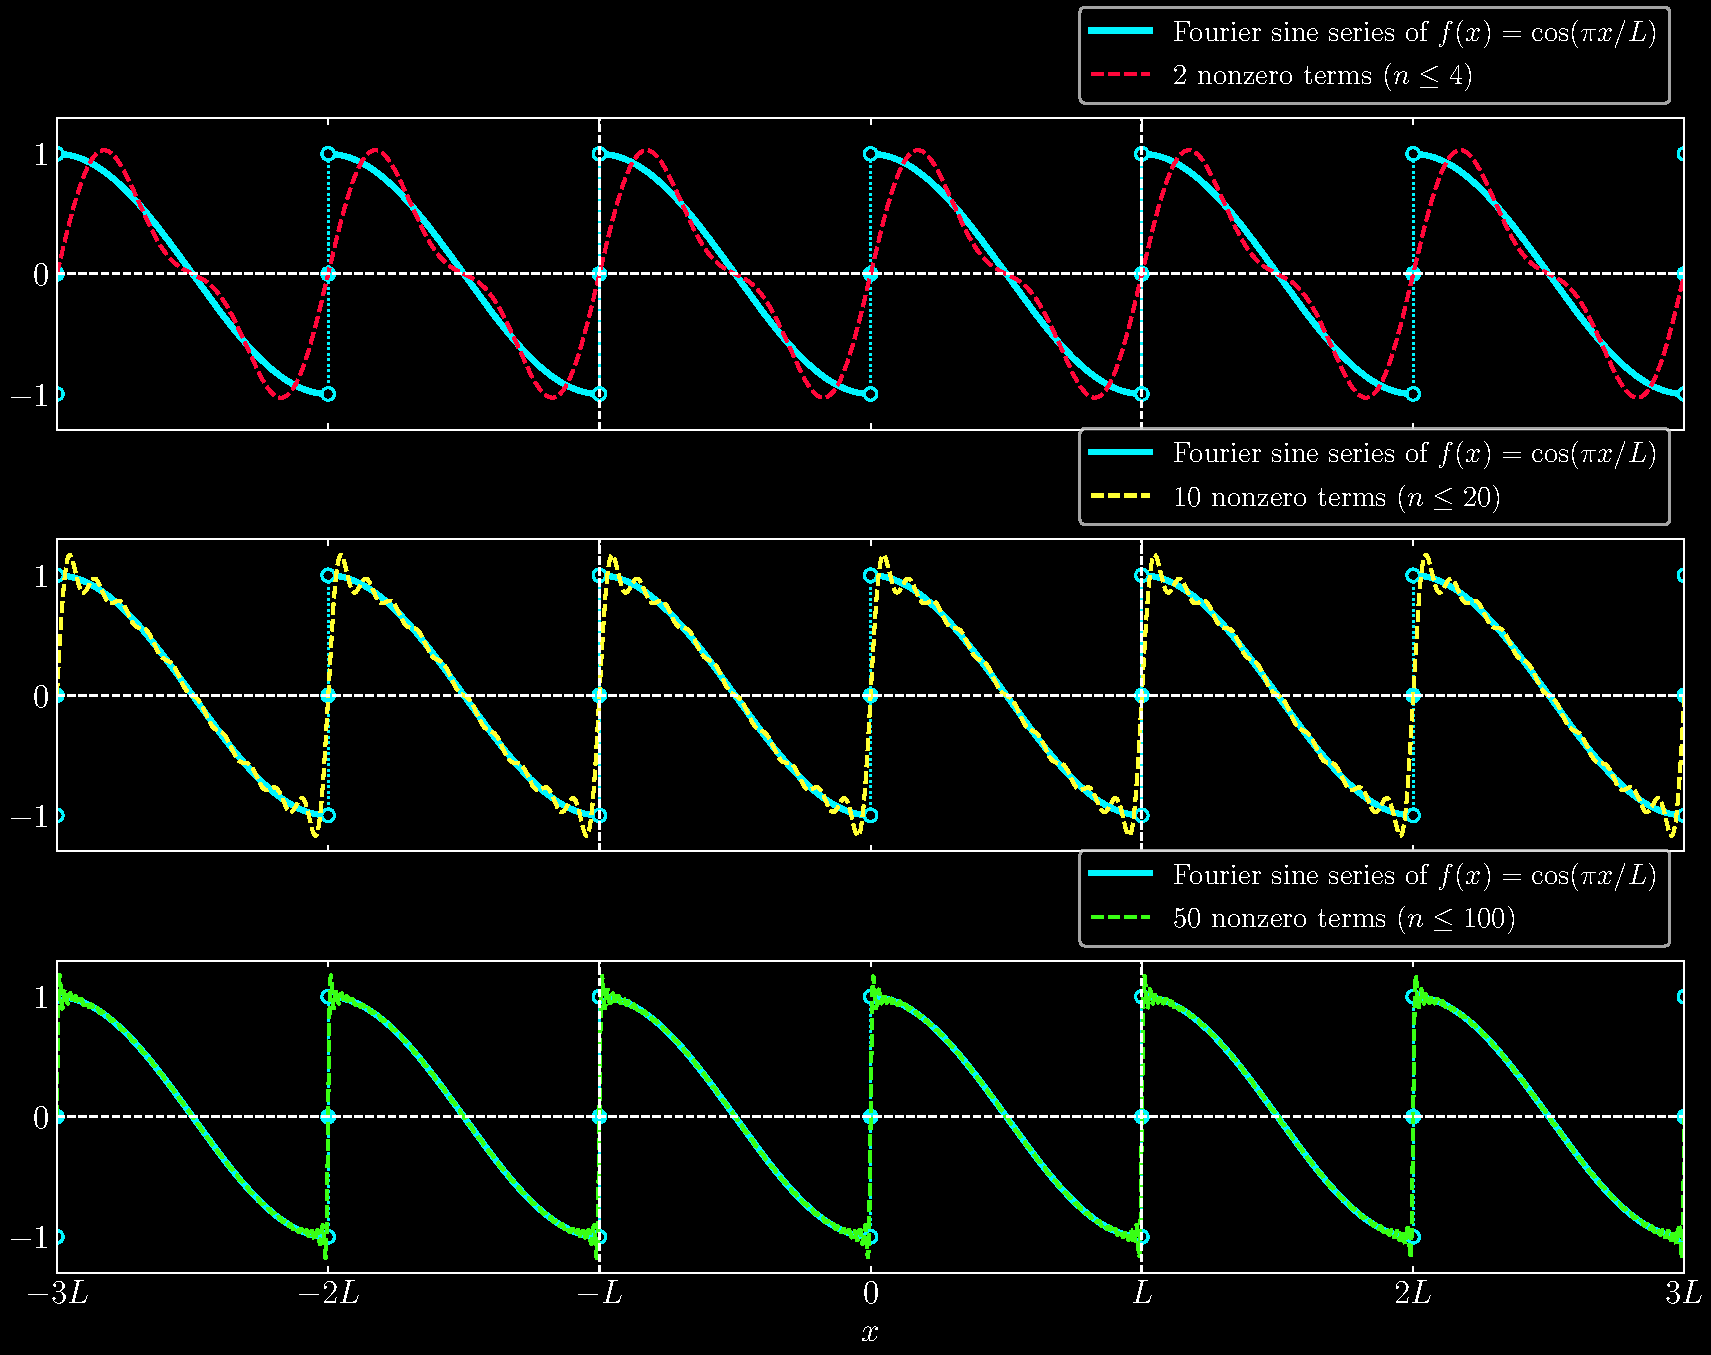
\includegraphics[width=0.9\textwidth]{../chap3/sec3.3/chap3sec3.3ex3a.pdf}
	\item
	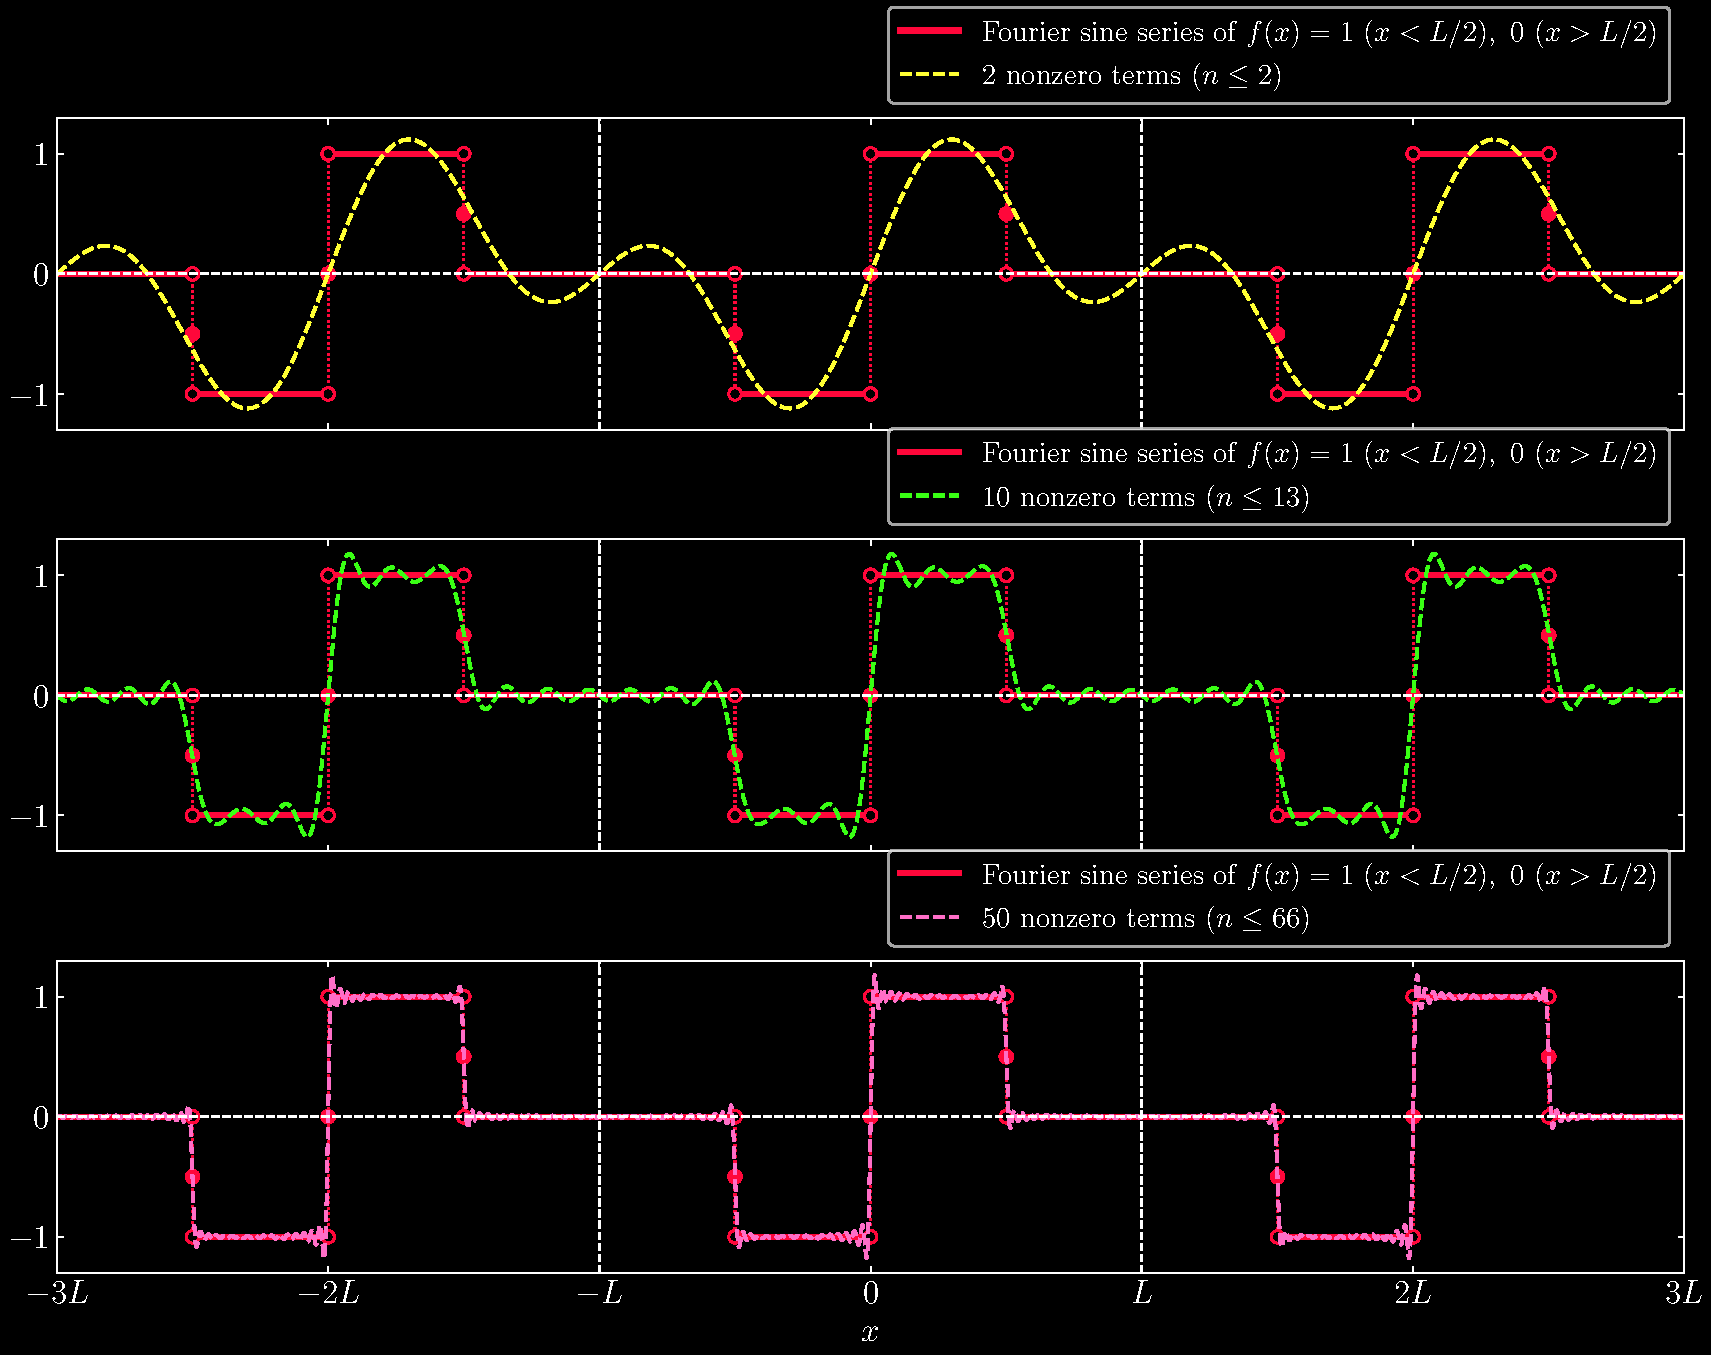
\includegraphics[width=0.9\textwidth]{../chap3/sec3.3/chap3sec3.3ex3b.pdf}
	\item
	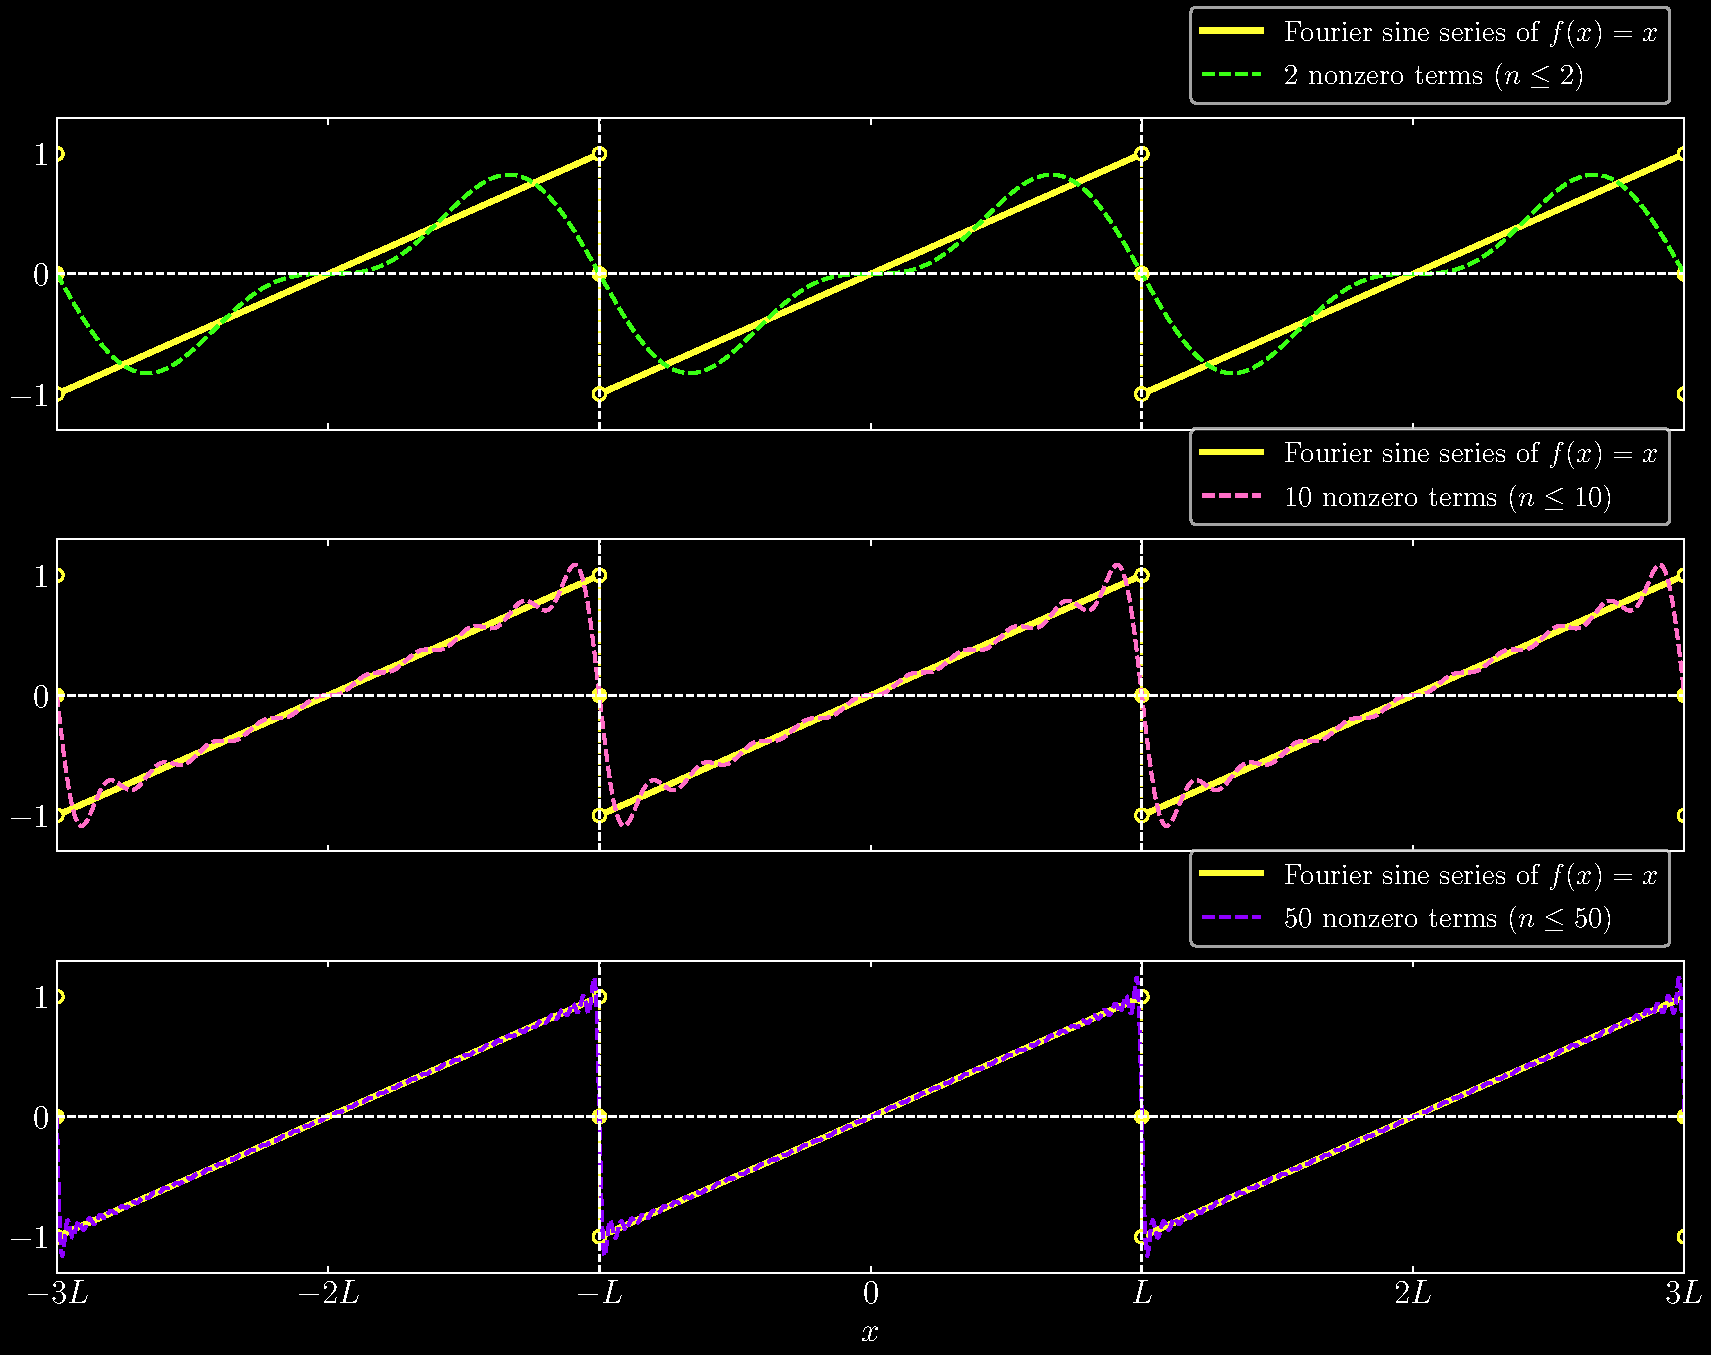
\includegraphics[width=0.9\textwidth]{../chap3/sec3.3/chap3sec3.3ex3c.pdf}
\end{enumerate}

\newpage
% QUESTION 4
\qs{3.3.4}{Sketch the Fourier cosine series of \( f \!\left( x \right) = \sin\!\left(\pi x / L\right) \). Briefly discuss.}

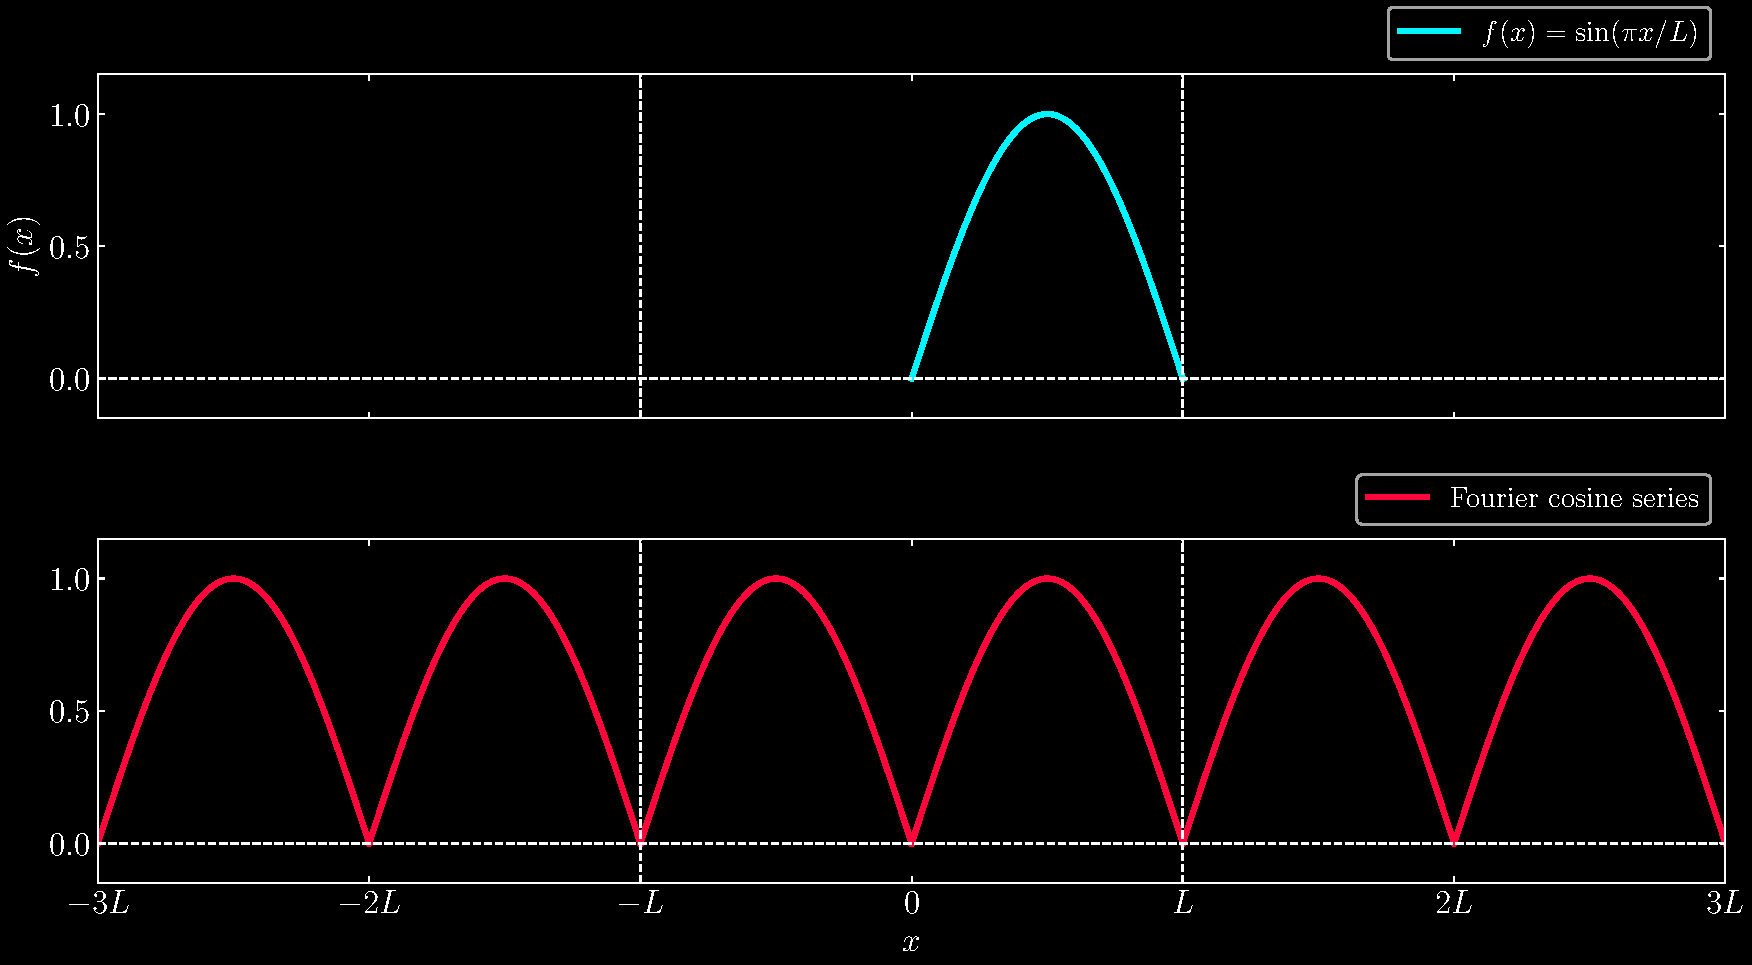
\includegraphics[width=1.0\textwidth]{../chap3/sec3.3/chap3sec3.3ex4.pdf}

\vspace{12pt}

The Fourier cosine series looks exactly like \( \abs{\sin\!\left(\pi x / L\right)} \), having period \( L \). If we were to actually derive the Fourier series (and thus the even extension of \( f \!\left( x \right) \)), we would find

\begin{align*}
	A_{0} & = \frac{1}{L}\int^{L}_{0} \sin\!\left(\frac{\pi x}{L}\right) \, dx \\
	 & = -\frac{1}{\pi}\cos\!\left(\frac{\pi x}{L}\right)\Big|^{L}_{0} \\ 
	 & = \frac{2}{\pi} \\
	A_{1} & = \frac{2}{L}\int^{L}_{0} \sin\!\left(\frac{\pi x}{L}\right)\cos\!\left(\frac{\pi x}{L}\right) \, dx \\
	      & = \frac{1}{L}\int^{L}_{0} \sin\!\left(\frac{2\pi x}{L}\right) \, dx \\
      & = -\frac{1}{2\pi}\cos\!\left(\frac{2\pi x}{L}\right)\Big|^{L}_{0} \\
      & = 0 \\
	A_{n} & = \frac{2}{L}\int^{L}_{0} \sin\!\left(\frac{\pi x}{L}\right)\cos\!\left(\frac{n \pi x}{L}\right) \, dx \\
	      & = \frac{1}{L}\int^{L}_{0} \left[\sin\!\left(\frac{(n+1) \pi x}{L}\right) - \sin\!\left(\frac{(n-1) \pi x}{L}\right)\right] dx \\
      & = \frac{1}{\pi}\left(1 + (-1)^{n}\right)\left[\frac{1}{n+1} - \frac{1}{n-1}\right] \\
      & = -\frac{2\left(1 + (-1)^n\right)}{\pi\left(n^2 - 1\right)}, \qquad n \neq 1
\end{align*}
for the \( A_{n} \), let \( n = 2m \) and reindex as 
\[
	A_{m} = -\frac{4}{\pi \!\left( 4m^{2} - 1 \right)} 
\]
which combine to produce
\[
	f \!\left( x \right) \sim \frac{2}{\pi} - \frac{4}{\pi}\sum^{\infty}_{m=1} \frac{\cos\!\left(2m \pi x / L\right)}{4m^{2} - 1}
\]
Observe the pattern: \textit{the Fourier cosine series consists only of even terms}. Moreover, since \( \sin\!\left(\pi x / L\right) = 0 \) at \( x = 0 \) and \( x = L \), the Fourier series converges to \( f \!\left( x \right) \) for \textit{all} \( x \) over \( \!\left[ 0,L \right] \), not only \( \!\left( 0,L \right) \). Crucially, \textbf{there is no Gibbs overshoot at the boundary}, as we have no jump discontinuity. \textbf{This is a crucial point and one I would advise the reader to internalize!}

\vspace{12pt}

% QUESTION 5
\qs{3.3.5}{For the following functions, sketch the Fourier cosine series of \( f \!\left( x \right) \) and determine its Fourier coefficients:
\begin{enumerate}[label=(\alph*)]
	\item \( f \!\left( x \right) = x^{2} \)
	\item \( f \!\left( x \right) = \begin{cases}
		1 & x < L/6 \\
		3 & L/6 < x < L/2 \\
		0 & x > L/2
	\end{cases} \)
	\item \( f \!\left( x \right) = \begin{cases}
		0 & x < L/2 \\
		x & x > L/2 
	\end{cases} \)
\end{enumerate}}

\begin{enumerate}[label=(\alph*)]
	\item \begin{align*}
		A_{0} & = \frac{1}{L}\int^{L}_{0} x^{2} \, dx \\
		 & = \frac{L^{2}}{3} \\ 
		A_{n} & = \frac{2}{L}\int^{L}_{0} x^{2}\cos\!\left(\frac{n \pi x}{L}\right) \, dx \\
		      & = \frac{2}{L}\left[ \frac{L}{n\pi}\,x^{2}\sin\!\left(\frac{n \pi x}{L}\right)\Big|^{L}_{0} - \frac{2L}{n\pi}\int^{L}_{0} x\sin\!\left(\frac{n \pi x}{L}\right) \, dx \right] \\
      & = -\frac{4}{n\pi}\left[ -\frac{L}{n\pi}\,x\cos\!\left(\frac{n \pi x}{L}\right)\Big|^{L}_{0} + \frac{L}{n\pi}\int^{L}_{0} \cos\!\left(\frac{n \pi x}{L}\right) \, dx \right] \\
      & = -\frac{4}{n\pi}\left[ -\frac{L^{2}(-1)^n}{n\pi} + 0 \right] \\
      & = \frac{4L^{2}(-1)^{n}}{n^{2}\pi^{2}}
	\end{align*}
	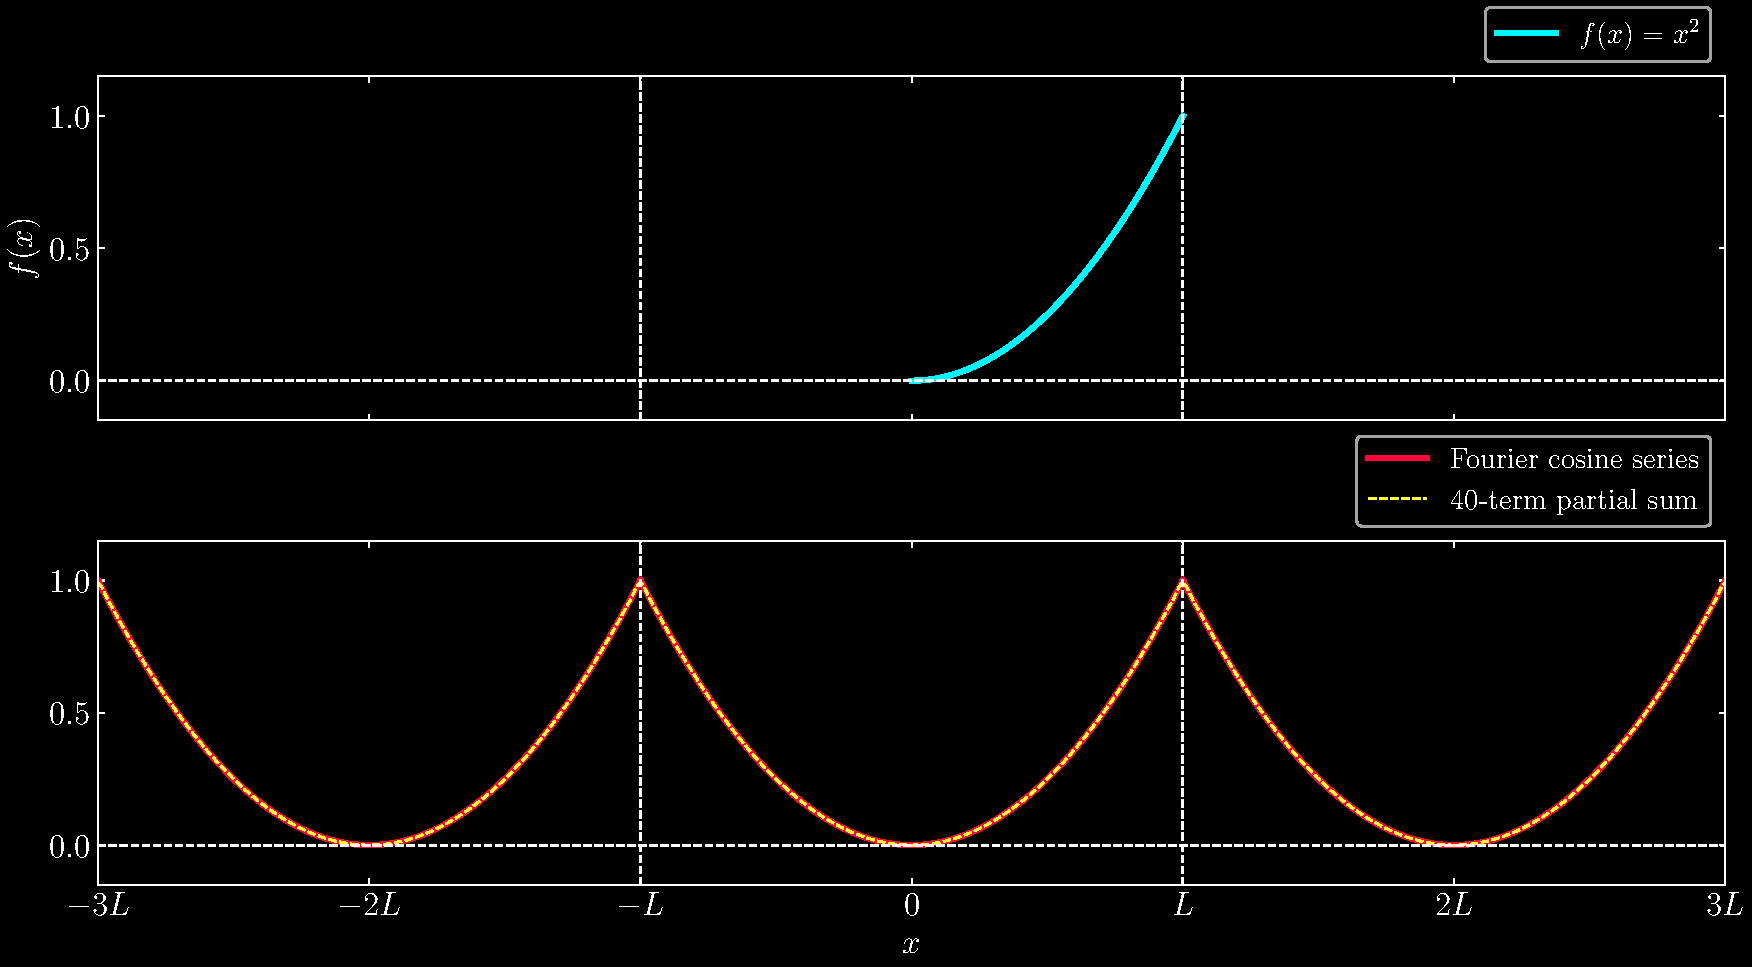
\includegraphics[width=1.0\textwidth]{../chap3/sec3.3/chap3sec3.3ex5a.pdf}
	\item \begin{align*}
			A_{0} & = \frac{1}{L}\!\left[ \int^{L/6}_{0} \, dx + \int^{L/2}_{L/6} 3 \, dx \right] \\
		 & = \frac{1}{L}\!\left( \frac{L}{6} + L \right) \\ 
		 & = \frac{7}{6} \\
		A_{n} & = \frac{2}{L}\!\left[ \int^{L/6}_{0} \cos\!\left(\frac{n \pi x}{L}\right) \, dx + 3\int^{L/2}_{L/6} \cos\!\left(\frac{n \pi x}{L}\right) \, dx \right] \\
      & = \frac{2}{n\pi}\left[ \sin\!\left(\frac{n \pi x}{L}\right)\Big|^{L/6}_{0} + 3\sin\!\left(\frac{n \pi x}{L}\right)\Big|^{L/2}_{L/6} \right] \\
      & = \frac{2}{n\pi}\left[ 3\sin\!\left(\frac{n\pi}{2}\right) - 2\sin\!\left(\frac{n\pi}{6}\right) \right]
	\end{align*}
	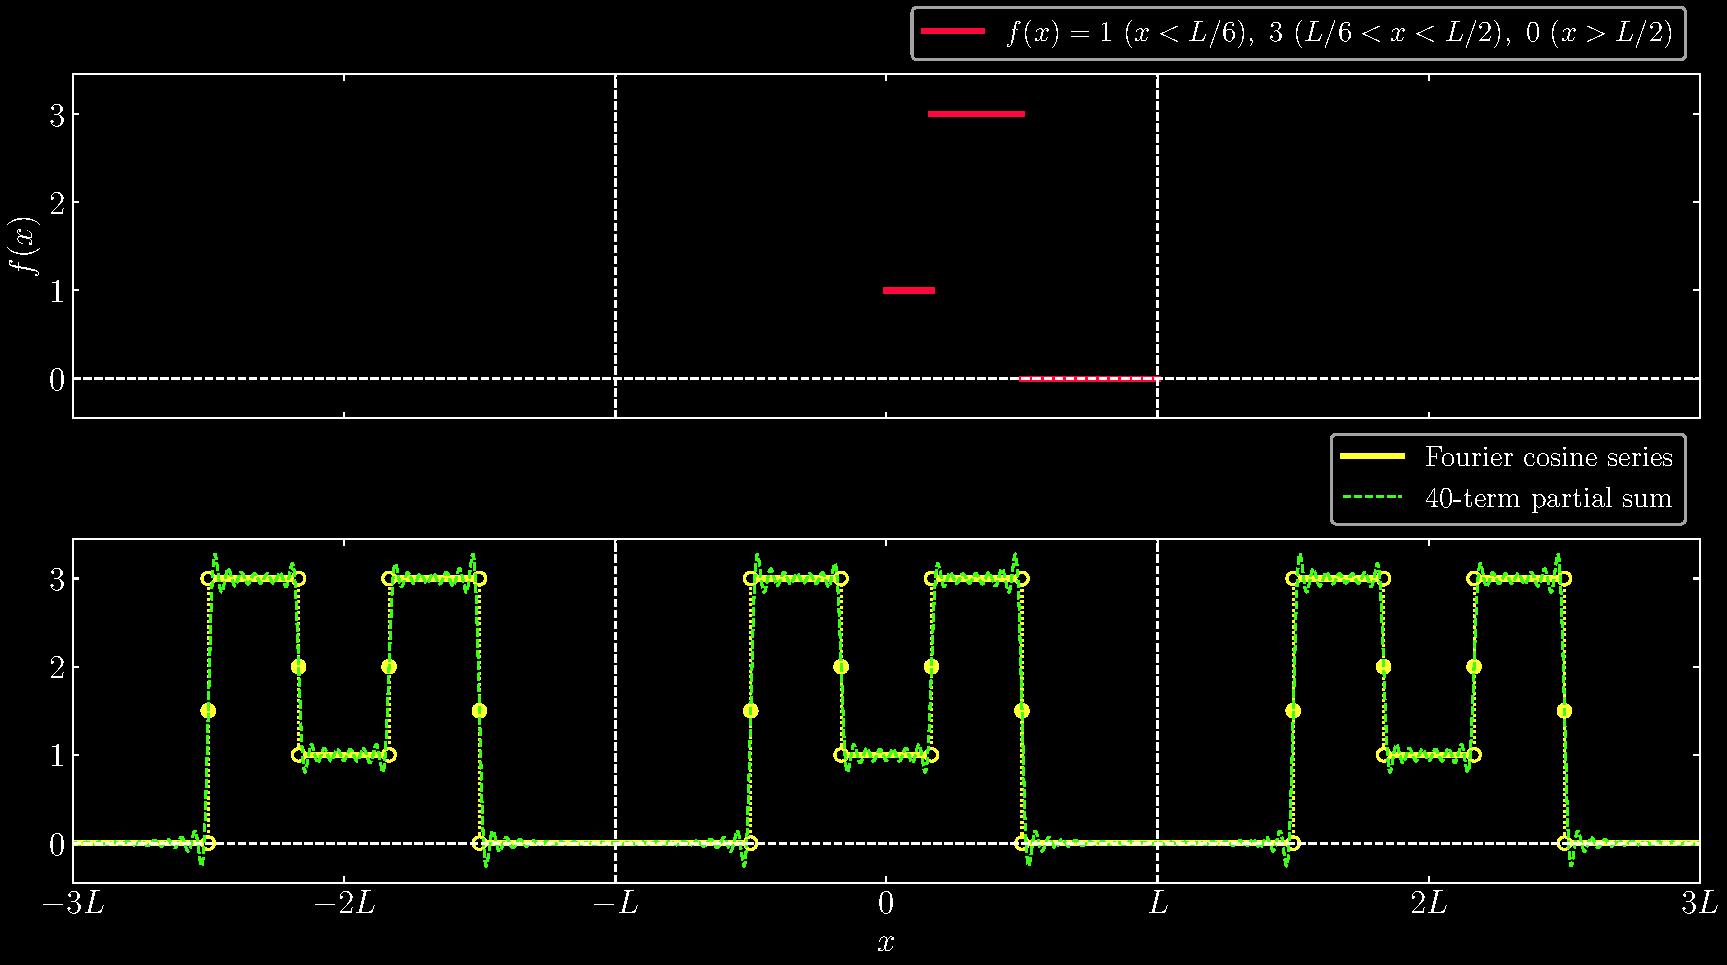
\includegraphics[width=1.0\textwidth]{../chap3/sec3.3/chap3sec3.3ex5b.pdf}
	\item \begin{align*}
		A_{0} & = \frac{1}{L}\int^{L}_{L/2} x \, dx \\
		 & = \frac{1}{L}\!\left( \frac{L^{2}}{2} - \frac{L^{2}}{8} \right) \\ 
		 & = \frac{3L}{8} \\
		A_{n} & = \frac{2}{L}\int^{L}_{L/2} x \cos\!\left(\frac{n \pi x}{L}\right) \, dx \\
		      & = \frac{2}{L}\left[ \frac{L}{n\pi}\,x\sin\!\left(\frac{n \pi x}{L}\right)\Big|^{L}_{L/2} - \frac{L}{n\pi}\int^{L}_{L/2} \sin\!\left(\frac{n \pi x}{L}\right) \, dx \right] \\
      & = \frac{2}{L}\left[ -\frac{L^{2}}{2n\pi}\sin\!\left(\frac{n\pi}{2}\right) + \frac{L^{2}}{n^{2}\pi^{2}}\cos\!\left(\frac{n \pi x}{L}\right)\Big|^{L}_{L/2} \right] \\
      & = -\frac{L}{n\pi}\sin\!\left(\frac{n\pi}{2}\right) + \frac{2L}{n^{2}\pi^{2}}\left[ (-1)^{n} - \cos\!\left(\frac{n\pi}{2}\right) \right]
	\end{align*}
	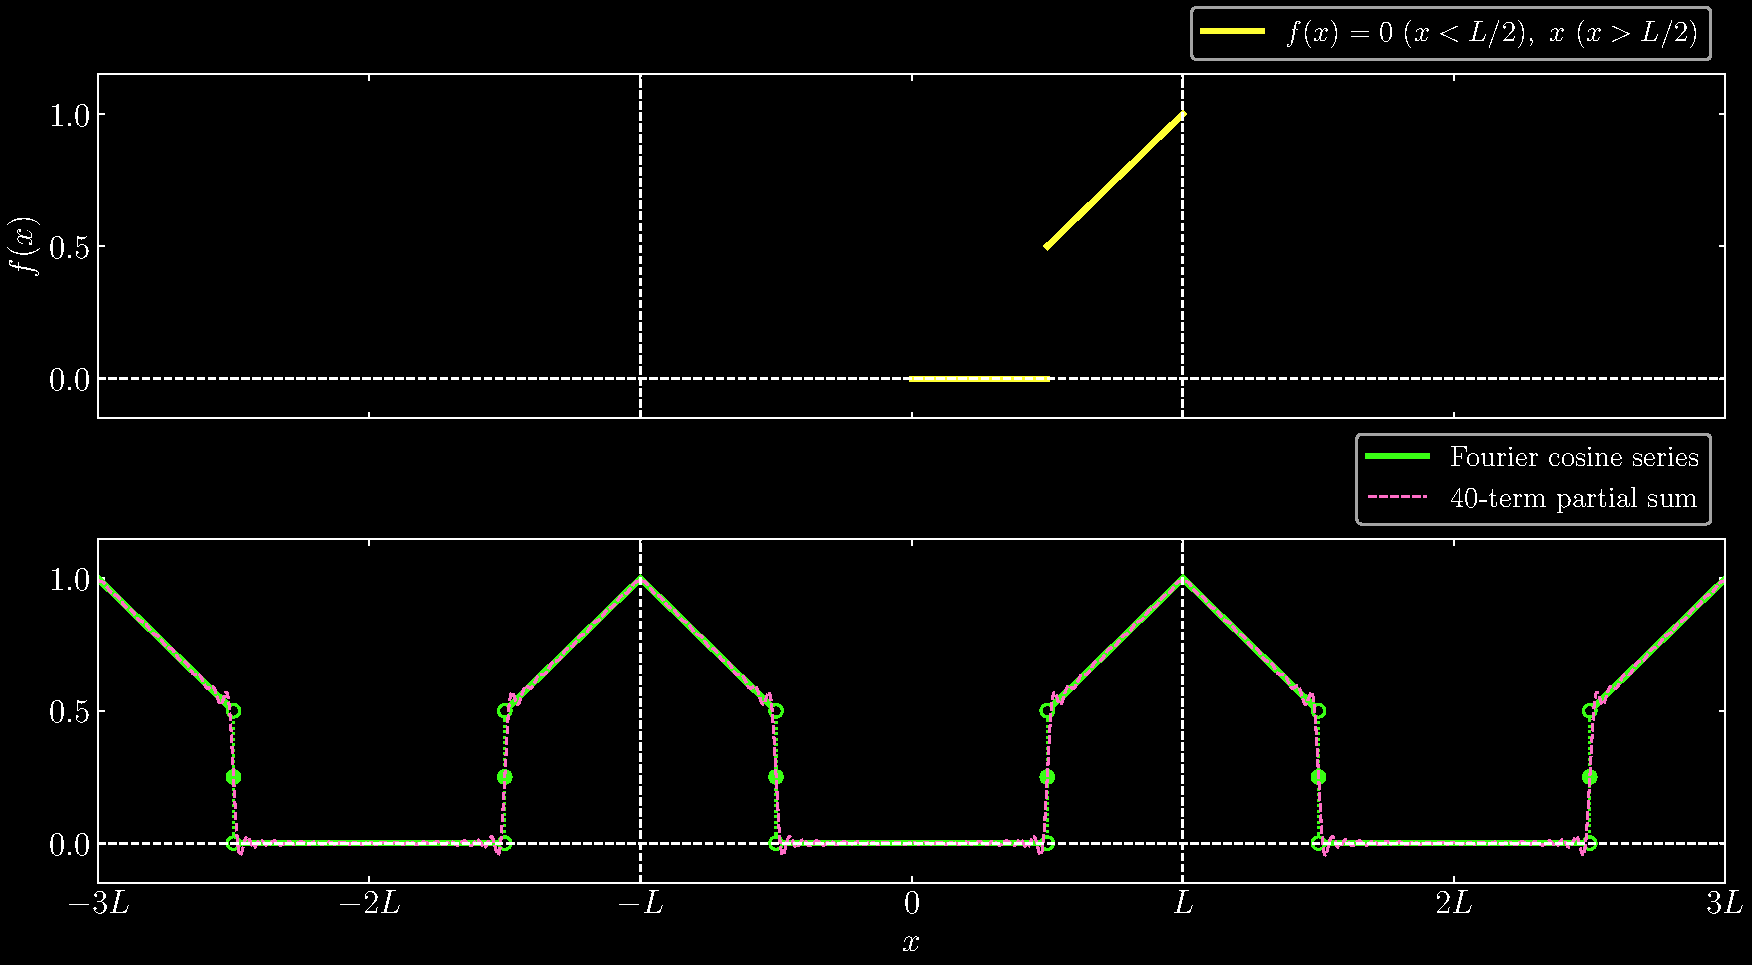
\includegraphics[width=1.0\textwidth]{../chap3/sec3.3/chap3sec3.3ex5c.pdf}
\end{enumerate}

\newpage
% QUESTION 6
\qs{3.3.6}{For the following functions, sketch the Fourier cosine series of \( f \!\left( x \right) \). Also, roughly sketch the sum of a finite number of nonzero terms (at least the first two) of the Fourier cosine series:
\begin{enumerate}[label=(\alph*)]
	\item \( f \!\left( x \right) = x \) [Use formulas (3.3.22) and (3.3.23)].
	\item \( f \!\left( x \right) = \begin{cases}
		0 & x < L/2 \\
		1 & x > L/2 
	\end{cases} \) [Use carefully formulas (3.2.6) and (3.2.7).]
	\item \( f \!\left( x \right) = \begin{cases}
		1 & x < L/2 \\
		0 & x > L/2 
	\end{cases} \) [\textit{Hint}: Add the functions in parts (b) and (c).]
\end{enumerate}}

Note that there is a typographical error in the text; what I have written here is the correct problem statement.

\begin{enumerate}[label=(\alph*)]
	\item \begin{align*}
		A_{0} & = \frac{1}{L}\int^{L}_{0} x \, dx \\
		 & = \frac{1}{L}\!\left( \frac{L^{2}}{2} \right) \\ 
		 & = \frac{L}{2} \\
		A_{n} & = \frac{2}{L}\int^{L}_{0} x \cos\!\left(\frac{n \pi x}{L}\right) \, dx \\
		      & = \frac{2}{L}\frac{L^{2}}{n^{2}\pi^{2}}\!\left[ \cos\!\left(\frac{n \pi x}{L}\right) + \frac{n \pi x}{L}\sin\!\left(\frac{n \pi x}{L}\right) \right]^{L}_{0} \\
		      & = \frac{2L}{\!\left( n \pi \right)^{2}}\!\left[ \cos\!\left(n \pi\right) - 1 \right]
	\end{align*}
	Since \( \cos\!\left(n \pi\right) - 1 \) is \( 0 \) for even \( n \) and \( -2 \) for odd \( n \), the even coefficients vanish and, writing \( n = 2m - 1 \),
	\[
		A_{2m-1} = -\frac{4L}{\pi^{2}\!\left( 2m-1 \right)^{2}} 
	\]
	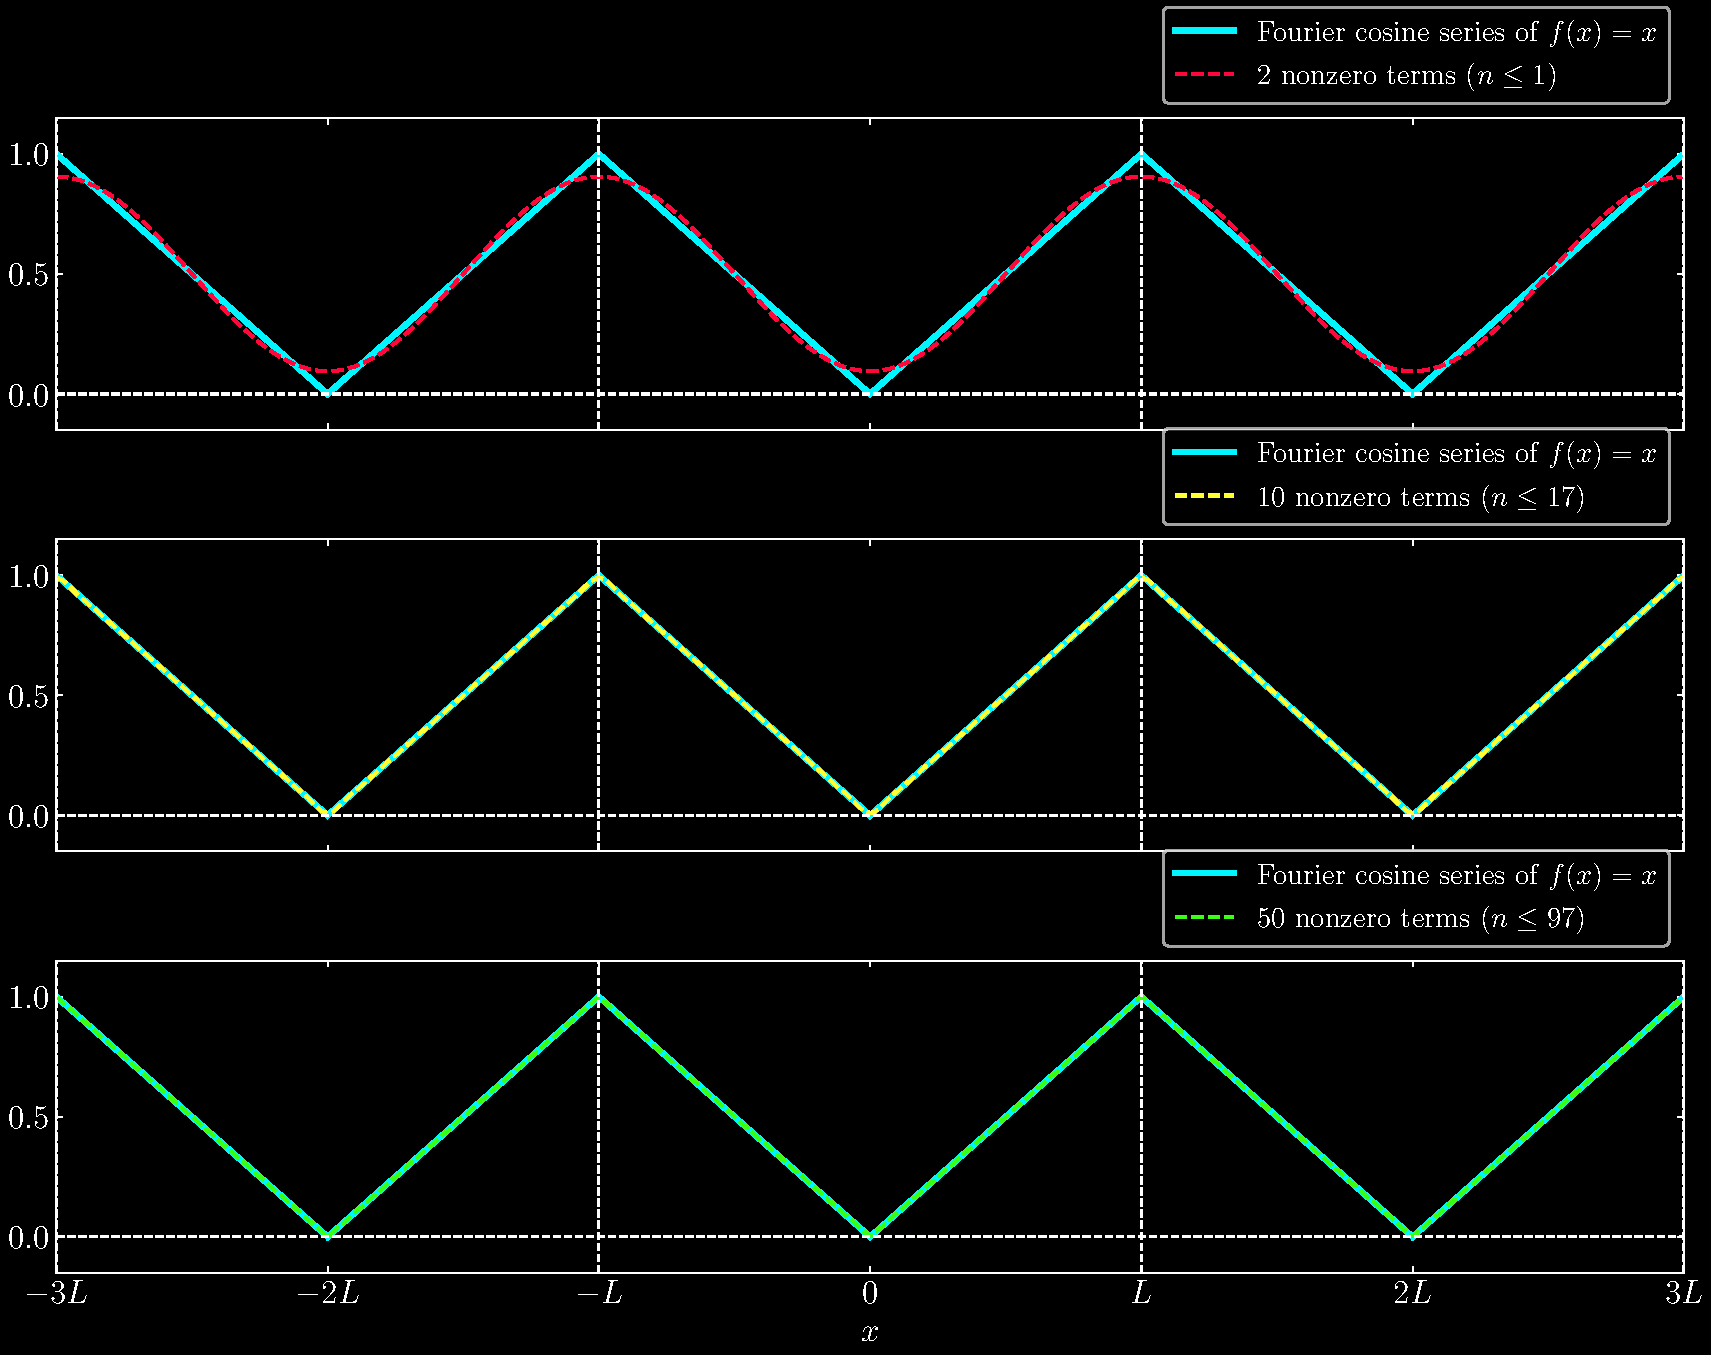
\includegraphics[width=0.9\textwidth]{../chap3/sec3.3/chap3sec3.3ex6a.pdf}
	\item \begin{align*}
		A_{0} & = \frac{1}{L}\int^{L}_{L/2} \, dx \\
		 & = \frac{1}{2} \\ 
		A_{n} & = \frac{2}{L}\int^{L}_{L/2} \cos\!\left(\frac{n \pi x}{L}\right) \, dx \\
		      & = \frac{2}{n \pi}\sin\!\left(\frac{n \pi x}{L}\right)\Big|^{L}_{L/2} \\
		      & = -\frac{2}{n \pi}\sin\!\left(\frac{n \pi}{2}\right)
	\end{align*}
	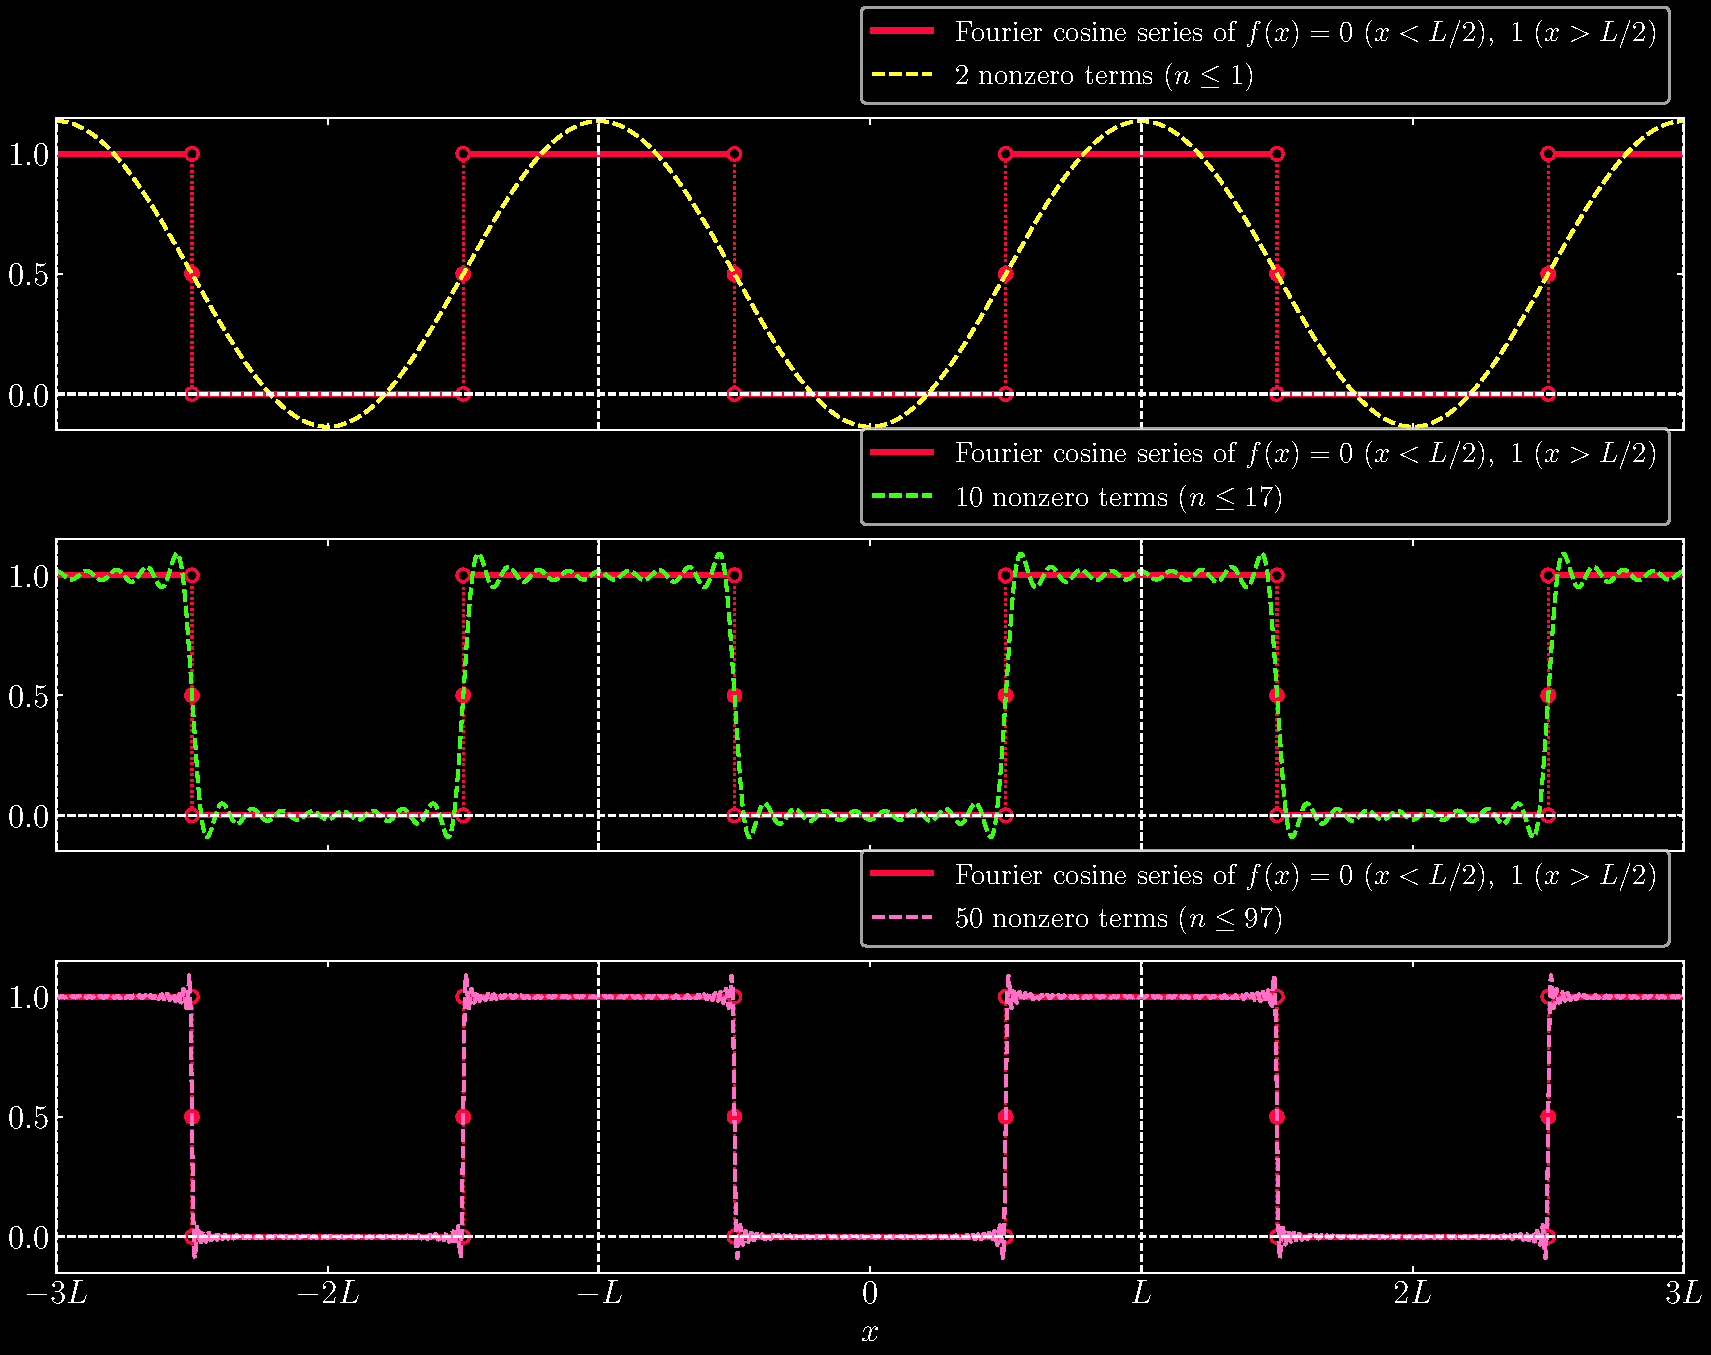
\includegraphics[width=0.9\textwidth]{../chap3/sec3.3/chap3sec3.3ex6b.pdf}
	\item \begin{align*}
		A_{0} & = \frac{1}{L}\int^{L/2}_{0} \, dx \\
		 & = \frac{1}{2} \\ 
		A_{n} & = \frac{2}{L}\int^{L/2}_{0} \cos\!\left(\frac{n \pi x}{L}\right) \, dx \\
		      & = \frac{2}{n \pi}\sin\!\left(\frac{n \pi x}{L}\right)\Big|^{L/2}_{0} \\
		      & = \frac{2}{n \pi}\sin\!\left(\frac{n \pi}{2}\right)
	\end{align*}
	Observe that adding the two Fourier series cancels the \( A_{n} \) terms from each, leaving only the \( A_{0} \) terms: \( 1/2 + 1/2 = 1 \).

	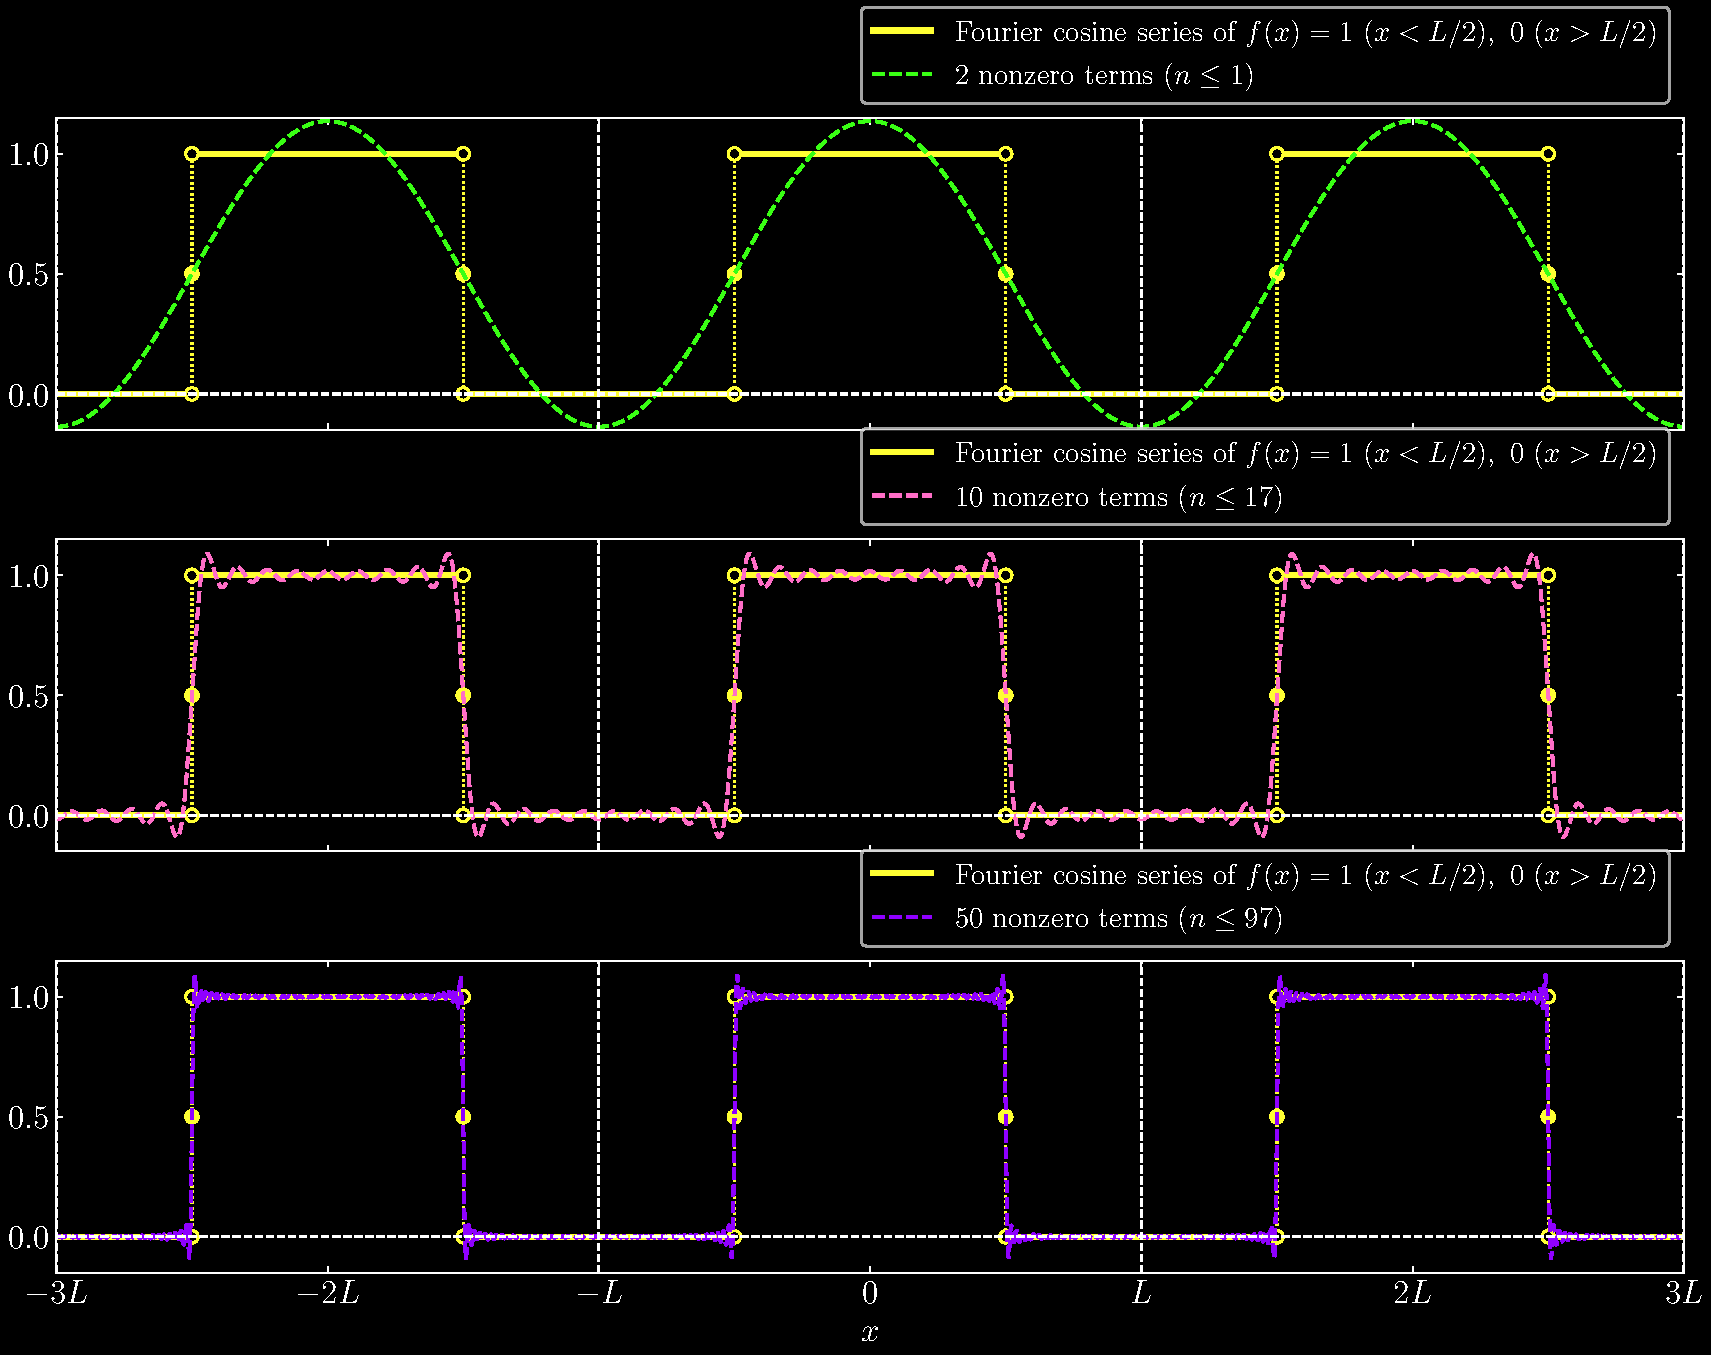
\includegraphics[width=0.9\textwidth]{../chap3/sec3.3/chap3sec3.3ex6c.pdf}
\end{enumerate}

% QUESTION 7
\qs{3.3.7}{Show that \( e^{x} \) is the sum of an even and an odd function.}
\[
	e^{x} = \underbrace{\frac{1}{2}\!\left( e^{x} + e^{-x} \right)}_{f_{\text{even}}} + \underbrace{\frac{1}{2}\!\left( e^{x} - e^{-x} \right)}_{f_{\text{odd}}} = \cosh\!\left(x\right) + \sinh\!\left(x\right)
\]
Observe that 
\[
	f_{\text{even}}\!\left( x \right) = \frac{1}{2}\!\left( e^{x} + e^{-x} \right) = \frac{1}{2}\!\left( e^{-x} + e^{x} \right) = f_{\text{even}}\!\left( -x \right) 
\]
and
\[
	f_{\text{odd}}\!\left( x \right) = \frac{1}{2}\!\left( e^{x} - e^{-x} \right) = -\frac{1}{2}\!\left( e^{-x} - e^{x} \right) = -f_{\text{odd}}\!\left( -x \right)
\]

\newpage
% QUESTION 8
\qs{3.3.8}{\begin{enumerate}[label=(\alph*)]
	\item Determine formulas for the even extension of any \( f \!\left( x \right) \). Compare to the formula for the even part of \( f \!\left( x \right) \).
	\item Do the same for the odd extension of \( f \!\left( x \right) \) and the odd part of \( f \!\left( x \right) \).
	\item Calculate and sketch the four functions of parts (a) and (b) if 
	\[
		f \!\left( x \right) = \begin{cases}
			x & x > 0 \\
			x^{2} & x < 0 
		\end{cases} 
	\]
	Graphically add the even and odd parts of \( f \!\left( x \right) \). What occurs? Similarly, add the even and odd extensions. What occurs then?
\end{enumerate}}

\begin{enumerate}[label=(\alph*)]
	\item The even extension of \( f \!\left( x \right) \) is given by
	\[
		f_{\text{even}}\!\left( x \right) = \begin{cases}
			f \!\left( x \right) & x > 0 \\
			f \!\left( -x \right) & x < 0 
		\end{cases} 
	\]
	As Haberman is emphatic about, do \textbf{not} confuse the even \textit{part} of \( f \!\left( x \right) \) with its \textit{extension}. They are equal, however, when \( f \!\left( x \right) \) is itself an even function. The part and extension differ in their construction: the extension performs a mirror reflection of \( f \!\left( x \right) \) about the vertical axis, while the part takes an arithmetic mean of \( f \!\left( x \right) \) evaluated at \textit{both} positive and negative \( x \).
	\item The odd extension of \( f \!\left( x \right) \) is given by
	\[
		f_{\text{odd}}\!\left( x \right) = \begin{cases}
			f \!\left( x \right) & x > 0 \\
			-f \!\left( -x \right) & x < 0 
		\end{cases} 
	\]
	Similarly, when \( f \!\left( x \right) \) is itself odd, the extension and part are equal. In their construction, the extension is a reflection through the origin (i.e. reflecting across the vertical axis \textit{and then} the horizontal axis), while the part is an arithmetic mean of \( f \!\left( x \right) \) and \( -f \!\left( -x \right) \).
	\item First, for clarity in evaluating \( f \!\left( -x \right) \), keep the following in mind: define \( y = -x \). When \( x < 0 \), then \( y > 0 \). When that is the case, \( f \!\left( y \right) = y = -x \). Alternatively, when \( x > 0 \), \( y < 0 \), and \(  f \!\left( y \right) = y^{2} = \!\left( -x \right)^{2} = x^{2} \).

	It is critical to not simply substitute in a negative sign in each branch. Instead, the sign of \( -x \) directs us to which case of \( f \!\left( x \right) \) we should be on.
	\[
		f \!\left( x \right) = \begin{cases}
			x & x > 0 \\
			x^{2} & x < 0 
		\end{cases},
		\quad
		f \!\left( -x \right) = \begin{cases}
			x^{2} & x > 0 \\
			-x & x < 0 
		\end{cases},
		\quad
		-f \!\left( -x \right) = \begin{cases}
			-x^{2} & x > 0 \\
			x & x < 0 
		\end{cases}
	\]
	Then we derive
	\begin{align*}
		f_{\text{even part}}\!\left( x \right) & = \frac{1}{2}\!\left( f \!\left( x \right) + f \!\left( -x \right) \right) =  \begin{cases}
			\frac{1}{2}\!\left( x + x^{2} \right) & x > 0 \\
			\frac{1}{2}\!\left( -x + x^{2} \right) & x < 0
		\end{cases} \\
		f_{\text{odd part}}\!\left( x \right) & = \frac{1}{2}\!\left( f \!\left( x \right) - f \!\left( -x \right) \right) = \begin{cases}
			\frac{1}{2}\!\left( x - x^{2} \right) & x > 0 \\
			\frac{1}{2}\!\left( x + x^{2} \right) & x < 0 
		\end{cases} \\ 
		f_{\text{even ext.}}\!\left( x \right) & = \begin{cases}
			x & x > 0 \\
			-x & x < 0 
		\end{cases} = \abs{x} \\
		f_{\text{odd ext.}}\!\left( x \right) & = \begin{cases}
			x & x > 0 \\
			x & x < 0 
		\end{cases} = x
	\end{align*}
	Adding the parts, we simply get back \( f \!\left( x \right) \), as expected. Adding the extensions produces
	\[
		f_{\text{even ext.}}\!\left( x \right) + f_{\text{odd ext.}}\!\left( x \right) = \begin{cases}
			2x & x > 0 \\
			0 & x < 0 
		\end{cases} 
	\]
	which we expect, as both extensions will agree on the \( x > 0 \) portion (in a sense, they double each other in the sum), but cancel each other out on the \( x < 0 \) portion, being mirror images of one another about the horizontal axis. See the graph below for all four equations and the sums of the parts and extensions graphed out alongside \( f \!\left( x \right) \).

	\vspace{12pt}
	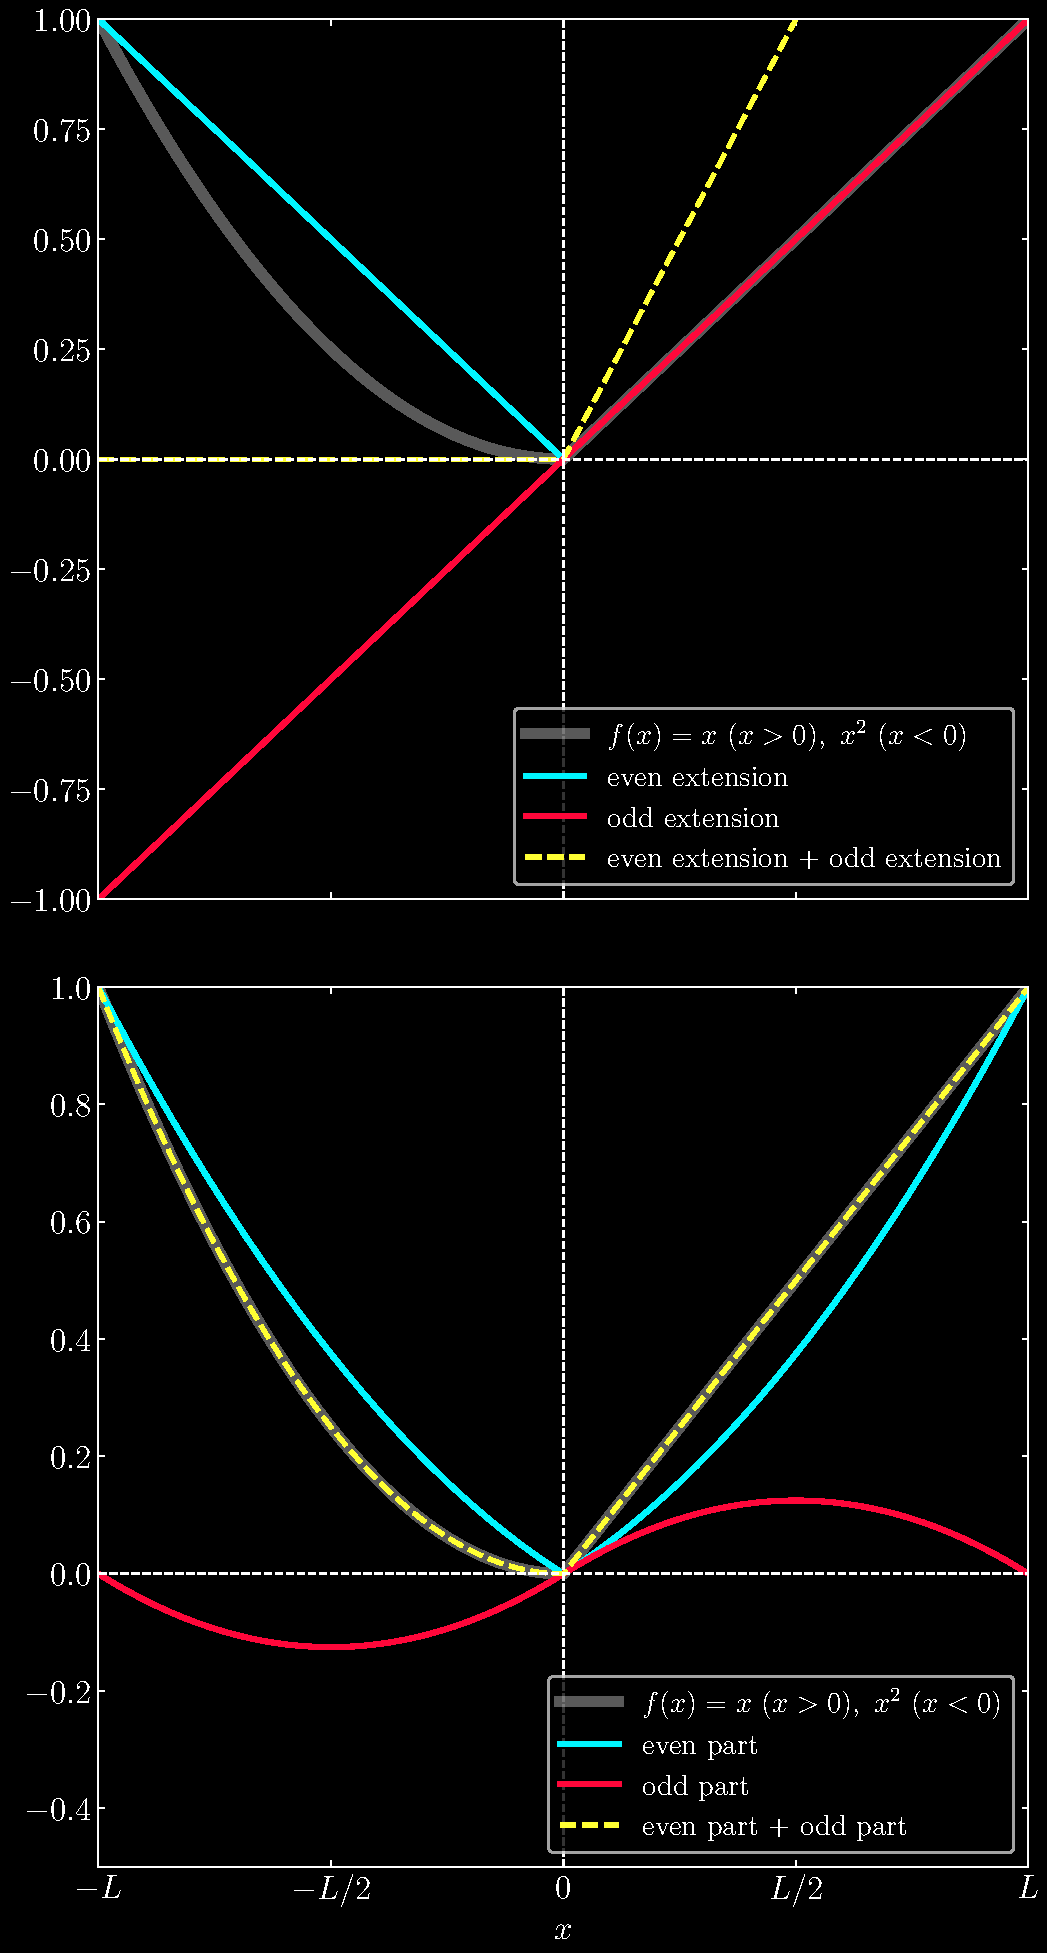
\includegraphics[width=1.0\textwidth]{../chap3/sec3.3/chap3sec3.3ex8c.pdf}
\end{enumerate}

% QUESTION 9
\qs{3.3.9}{What is the sum of the Fourier sine series of \( f \!\left( x \right) \) and the Fourier cosine series of \( f \!\left( x \right) \)? [What is the sum of the even and odd extensions of \( f \!\left( x \right) \)?]}

Akin to our solution from 3.3.8(c), the sum of the Fourier sine and cosine series will converge to 
\[
	g \!\left( x \right) = \begin{cases}
		2f \!\left( x \right) & 0 < x < L \\
		0 & -L < x < 0
	\end{cases} 
\]
and extended with period \( 2L \). This parallels the \( x < 0 \) segment vanishing in the previous problem. From the convergence theorem, we know that at the endpoints, the series converges to the arithmetic mean of \( g \!\left( x^{+} \right) \) and \( g \!\left( x^{-} \right) \).

\vspace{12pt}

% QUESTION 10
\qs{3.3.10}{If \( f \!\left( x \right) = \displaystyle{\begin{cases}
	x^{2} & x < 0 \\
	e^{-x} & x > 0 
\end{cases}} \), what are the even and odd parts of \( f \!\left( x \right) \)?}

When \( x < 0 \), then \( y = -x > 0 \), and \( f \!\left( y \right) = e^{y} = e^{x} \). Additionally, when \( x > 0 \), \( y = -x < 0 \), and \( f \!\left( y \right) = y^{2} = \!\left( -x \right)^{2} = x^{2} \). With these insights we can conclude
\[
	f \!\left( -x \right) = \begin{cases}
		e^{x} & x < 0 \\
		x^{2} & x > 0 
	\end{cases}, \qquad 
	-f \!\left( -x \right) = \begin{cases}
		-e^{x} & x < 0 \\
		-x^{2} & x > 0 
	\end{cases}
\]
Then we can compute 
\begin{alignat*}{2}
	f_{\text{even}}\!\left( x \right) & = \begin{cases}
		\frac{1}{2}\!\left( x^{2} + e^{x} \right) & x < 0 \\
		\frac{1}{2}\!\left( x^{2} + e^{-x} \right) & x > 0 
	\end{cases} && = \frac{1}{2}\!\left( x^{2} + e^{-\abs{x}} \right) \\
	f_{\text{odd}}\!\left( x \right) & = \begin{cases}
		\frac{1}{2}\!\left( x^{2} - e^{x} \right) & x < 0 \\
		\frac{1}{2}\!\left( -x^{2} + e^{-x} \right) & x > 0 
	\end{cases} && = \frac{1}{2}\text{sgn}\!\left( x \right)\!\left( e^{-\abs{x}} - x^{2} \right)
\end{alignat*}
As we anticipate, \( f_{\text{even}} + f_{\text{odd}} = f \).

\vspace{12pt}

% QUESTION 11
\qs{3.3.11}{Given a sketch of \( f \!\left( x \right) \), describe a procedure to sketch the even and odd parts of \( f \!\left( x \right) \).}

For the even part:
\begin{enumerate}[label=(\arabic*)]
	\item Draw the mirror image of \( f \!\left( x \right) \) about the vertical axis.
	\item Draw the even part, which is the vertical average of the original function and its mirror.
\end{enumerate}

For the odd part:
\begin{enumerate}[label=(\arabic*)]
	\item Rotate the graph of \( f \!\left( x \right) \) by \( 180^{\circ} \); that is what the mirror image of \( f \!\left( x \right) \) looks like on the original plot.
	\item Draw the odd part, which is the vertical average of the original function and its mirror.
\end{enumerate}

% QUESTION 12
\qs{3.3.12}{\begin{enumerate}[label=(\alph*)]
	\item Graphically show that the even terms (\( n \) even) of the Fourier sine series of any function on \( 0 \le x \le L \) are odd (antisymmetric) around \( x = L/2 \).
	\item Consider a function \( f \!\left( x \right) \) that is odd around \( x = L/2 \). Show that the odd coefficients (\( n \) odd) of the Fourier sine series of \( f \!\left( x \right) \) on \( 0 \le x \le L \) are zero.
\end{enumerate}}

\begin{enumerate}[label=(\alph*)]
	\item 
	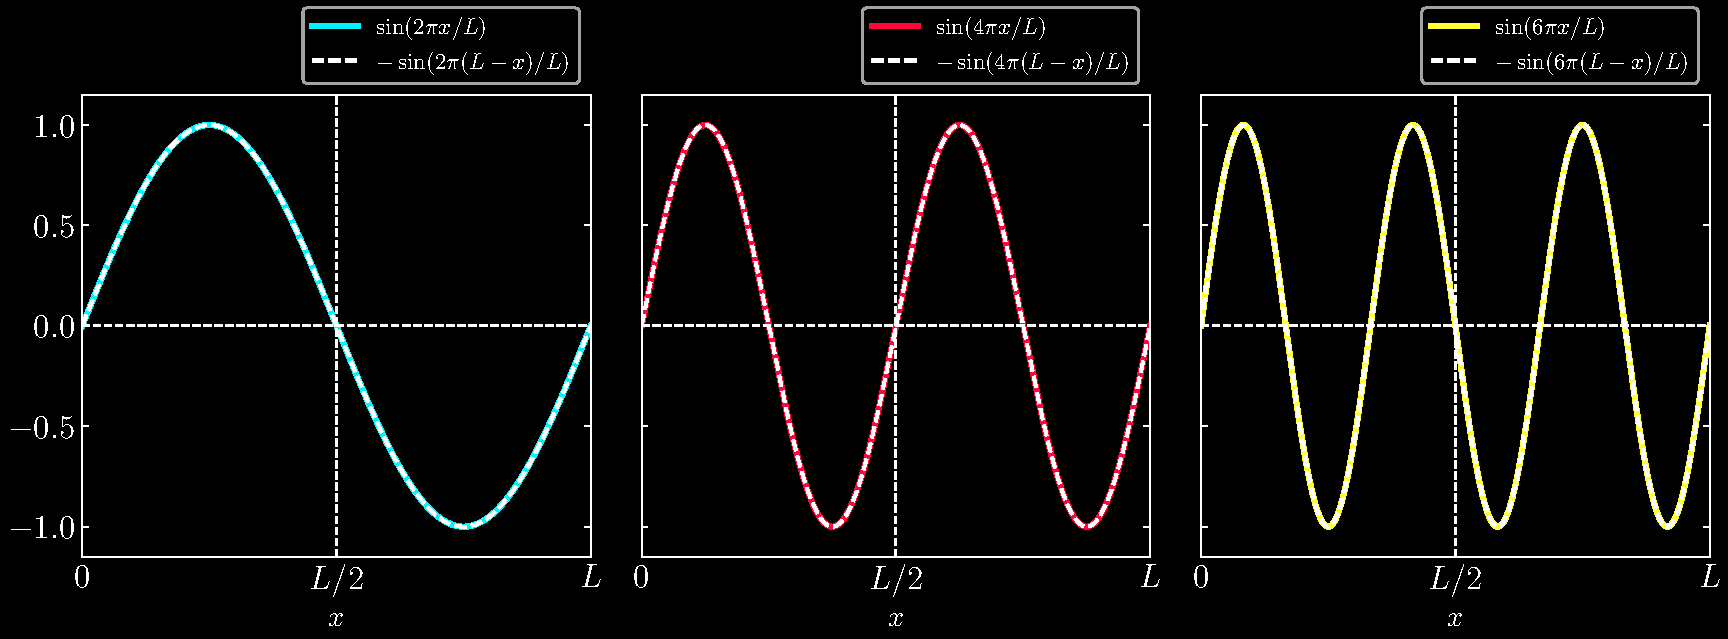
\includegraphics[width=0.9\textwidth]{../chap3/sec3.3/chap3sec3.3ex12a.pdf}
	\item The coefficients are given by 
	\[
		B_{n} = \frac{2}{L}\int^{L}_{0} f \!\left( x \right)\sin\!\left(\frac{n \pi x}{L}\right) \, dx 
	\]
	By premise, over \( \!\left[ 0,L \right] \), \( f \!\left( x \right) \) is odd about \( x = L/2 \). We wish to establish that for \( n \) odd, \( \sin\!\left(n \pi x / L\right) \) is even about \( L/2 \), as that would mean the integrand \( f \!\left( x \right)\sin\!\left(n \pi x / L\right) \) is odd about \( L/2 \) and vanishes when integrated over the symmetric interval \( \!\left[ 0,L \right] \). Equivalently, we can demonstrate that
	\[
		g \!\left( x \right) = \sin\!\left[\frac{n \pi}{L}\!\left( x + \frac{L}{2} \right)\right]
	\]
	is even about the origin. Let \( n = 2m + 1 \), \( m = 0, 1, ... \) and derive
	\begin{align*}
		g \!\left( x \right) & = \sin\!\left[\frac{\!\left( 2m + 1 \right)\pi}{L}\!\left( x + \frac{L}{2} \right)\right] = \sin\!\left[\frac{\!\left( 2m + 1 \right)\pi x}{L} + \frac{\!\left( 2m + 1 \right)\pi}{2} \right] \\
				     & = \!\left( -1 \right)^{m}\cos\!\left[\frac{\!\left( 2m + 1 \right)\pi x}{L}\right]
	\end{align*}
	Since cosine is even about the origin, we must also have \( g \!\left( x \right) \) is even, proving the result.
\end{enumerate}

% QUESTION 13
\qs{3.3.13}{Consider a function \( f \!\left( x \right) \) that is even around \( x = L/2 \). Show that the even coefficients (\( n \) even) of the Fourier sine series of \( f \!\left( x \right) \) on \( 0 \le x \le L \) are zero.}

The coefficients are given by
\[
	B_{n} = \frac{2}{L}\int^{L}_{0} f \!\left( x \right)\sin\!\left(\frac{n \pi x}{L}\right) \, dx  
\]
By premise, over \( \!\left[ 0,L \right] \), \( f \!\left( x \right) \) is even about \( x = L/2 \). The objective is to demonstrate that when \( n \) is even, \( f \!\left( x \right)\sin\!\left(n \pi x / L\right) \) is odd about \( x = L/2 \). Equivalently, we need only prove that \( \sin\!\left(n \pi
 x / L\right) \) is odd about that point (since an even times an odd function is odd), and an even easier way to frame this is to show that
\[
	g \!\left( x \right) = \sin\!\left[\frac{n \pi}{L}\!\left( x + \frac{L}{2} \right)\right]
\]
is odd about the origin. Let \( n = 2m \) and rewrite as 
\[
	g \!\left( x \right) = \sin\!\left[\frac{2m \pi}{L}\!\left( x + \frac{L}{2}\right)\right] = \sin\!\left(\frac{2m \pi x}{L} + m \pi\right) = \!\left( -1 \right)^{m}\sin\!\left(\frac{2m \pi x}{L}\right)
\]
Immediately we can deduce
\[
	g \!\left( -x \right) = \!\left( -1 \right)^{m + 1}\sin\!\left(\frac{2m \pi x}{L}\right) \implies -g \!\left( -x \right) = \!\left( -1 \right)^{m}\sin\!\left(\frac{2m \pi x}{L}\right) = g \!\left( x \right)
\]
Proving that \( g \!\left( x \right) \) is odd. Given that the integrand is established to be odd about \( x = L/2 \) for even \( n \), by symmetry of \( \!\left[ 0,L \right] \) about \( L/2 \), we have proven that \( B_{n} = 0 \).

\vspace{12pt}

% QUESTION 14
\qs{3.3.14}{\begin{enumerate}[label=(\alph*)]
	\item Consider a function \( f \!\left( x \right) \) that is even around \( x = L/2 \). Show that the odd coefficients (\( n \) odd) of the Fourier cosine series of \( f \!\left( x \right) \) on \( 0 \le x \le L \) are zero.
	\item Explain the result of part (a) by considering a Fourier cosine series of \( f \!\left( x \right) \) on the interval \( 0 \le x \le L/2 \).
\end{enumerate}}

\begin{enumerate}[label=(\alph*)]
	\item The coefficients are given by
	\[
		A_{n} = \frac{2}{L}\int^{L}_{0} f \!\left( x \right)\cos\!\left(\frac{n \pi x}{L}\right) \, dx 
	\]
	By premise, over \( \!\left[ 0,L \right] \), \( f \!\left( x \right) \) is even about \( x = L/2 \). We wish to prove that when \( n \) is odd, \( f \!\left( x \right)\cos\!\left(n \pi x / L\right) \) is odd about \( L/2 \). Put differently, we must prove that \( \cos\!\left(n \pi x / L\right) \) is odd about that point, or equivalently
	\[
		g \!\left( x \right) = \cos\!\left[\frac{n \pi}{L}\!\left( x + \frac{L}{2} \right)\right] 
	\]
	is odd about the origin. Let \( n = 2m + 1 \), \( m = 0,1,... \) and deduce
	\begin{align*}
		g \!\left( x \right) & = \cos\!\left[\frac{\!\left( 2m + 1 \right)\pi}{L}\!\left( x + \frac{L}{2} \right)\right] = \cos\!\left[\frac{\!\left( 2m + 1 \right)\pi x}{L} + \frac{\!\left( 2m + 1 \right)\pi}{2}\right] \\
				     & = \!\left( -1 \right)^{m + 1}\sin\!\left[\frac{\!\left( 2m + 1 \right)\pi x}{L}\right]
	\end{align*}
	and since sine is odd, we must also have \( g \!\left( x \right) \) is odd, establishing the result.
	\item It is good to motivate some geometric intuition: since \( f \!\left( x \right) \) is even about \( L/2 \), we know that the segments on \( \!\left[ 0,L/2 \right] \) and \( \!\left[ L/2,L \right] \) are mirror images of each other around \( x = L/2 \). If we replace the interval with \( \!\left[ 0,L/2 \right] \), our coefficients are written as 
	\[
		A_{n} = \frac{4}{L}\int^{L/2}_{0} f \!\left( x \right)\cos\!\left(\frac{2n \pi x}{L}\right) \, dx  
	\]
	In particular, observe that the basis functions \( \cos\!\left(2n \pi x / L\right) \) are only the even modes. The odd modes are nowhere to be found, which comports with our result from part (a). The Fourier cosine series built from these coefficients converges to \( f \!\left( x \right) \) on \( \!\left[ 0,L/2 \right] \). But we get two for the price of one: convince yourself that when we horizontally shift the cosine to the left by \( L/2 \), we can see that
	\[
		g \!\left( x \right) = \cos\!\left[\frac{2n \pi}{L}\!\left( x + \frac{L}{2} \right)\right] = \cos\!\left(\frac{2n \pi x}{L} + n \pi\right) = \!\left( -1 \right)^{n}\cos\!\left(\frac{2n \pi x}{L}\right)
	\]
	is even about the origin; by the translation, we can immediately deduce that \( \cos\!\left(2n \pi x / L\right) \) is even about \( L/2 \). Since both \( f \!\left( x \right) \) and the cosine basis functions are even about that point, \( A_{n} \) is exactly the same over \( \!\left[ 0,L/2 \right] \) \textit{and} \( \!\left[ L/2,L \right] \), and by even symmetry, \( \int^{L}_{0} = 2\int^{L/2}_{0}  \). This establishes
	\begin{align*}
		\frac{2}{L}\int^{L}_{0} f \!\left( x \right)\cos\!\left(\frac{2n \pi x}{L}\right) \, dx & = \frac{4}{L}\int^{L/2}_{0} f \!\left( x \right)\cos\!\left(\frac{2n \pi x}{L}\right) \, dx \\
													& = \frac{4}{L}\int^{L}_{L/2} f \!\left( x \right)\cos\!\left(\frac{2n \pi x}{L}\right) \, dx    
	\end{align*}
	where the left side includes only the even modes that match term-by-term with \( A_{n} \), proving that the odd modes must vanish as we established in part (a).
\end{enumerate}

% QUESTION 15
\qs{3.3.15}{Consider a function \( f \!\left( x \right) \) that is odd around \( x = L/2 \). Show that the even coefficients (\( n \) even) of the Fourier cosine series of \( f \!\left( x \right) \) on \( 0 \le x \le L \) are zero.}

The coefficients are given by
\[
	A_{n} = \frac{2}{L}\int^{L}_{0} f \!\left( x \right)\cos\!\left(\frac{n \pi x}{L}\right) \, dx 
\]
Our objective is to prove that \( f \!\left( x \right)\cos\!\left(n \pi x / L\right) \) is odd about \( L/2 \). By premise, \( f \!\left( x \right) \) is odd around that point, so we need only prove that \( \cos\!\left(n \pi x / L\right) \) is even about \( L/2 \). Equivalently, prove
\[
	g \!\left( x \right) = \cos\!\left[\frac{n \pi}{L}\!\left( x + \frac{L}{2} \right)\right]
\]
is even about the origin. Let \( n = 2m \) and deduce
\[
	g \!\left( x \right) = \cos\!\left(\frac{2m \pi x}{L} + m \pi \right) = \!\left( -1 \right)^{m}\cos\!\left(\frac{2m \pi x}{L}\right)
\]
Since cosine is even about the origin, so is \( g \!\left( x \right) \). Then \( f \!\left( x \right)\cos\!\left(n \pi x / L\right) \) is odd about \( L/2 \), and by symmetry of \( \!\left[ 0,L \right] \) around that point, \( A_{n} \) vanishes for all even \( n \).

\vspace{12pt}

% QUESTION 16
\qs{3.3.16}{Fourier series can be defined on other intervals besides \( -L \le x \le L \). Suppose that \( g \!\left( y \right) \) is defined for \( a \le y \le b \). Represent \( g \!\left( y \right) \) using periodic trigonometric functions with period \( b - a \). Determine formulas for coefficients. [\textit{Hint}: Use the linear transformation
\[
	y = \frac{a + b}{2} + \frac{b - a}{2L}x.] 
\]}

First, let us experiment with the book's hint for \( y \). Observe that \( y \!\left( L \right) = b \) and \( y \!\left( -L \right) = a \). Structurally, it is a sum of the average of the \( y \)-endpoints and a scaling term transforming between the \( 2L \) and \( b - a \) periods.

Expressing in terms of \( x \), do some algebraic manipulation to derive
\[
	x = \!\left( \frac{a + b}{a - b} \right)L + \frac{2L}{b - a}y
\]
where the differentials are related by
\[
	dx = \frac{2L}{b - a}dy
\]
Substituting into our full Fourier series, we have
\begin{align*}
	g \!\left( y \right) & \sim A_{0} + \sum^{\infty}_{n=1} A_{n}\cos\!\left[n \pi \!\left( \frac{a + b}{a - b} + \frac{2}{b - a}y \right) \right] + \sum^{\infty}_{n=1} B_{n}\sin\!\left[n \pi \!\left( \frac{a + b}{a - b} + \frac{2}{b - a}y \right) \right] \\
			     & \sim  A_{0} + \sum^{\infty}_{n=1} A_{n}\cos\!\left[ \frac{2n \pi}{b - a}\!\left( y - \frac{a + b}{2} \right) \right] + \sum^{\infty}_{n=1} B_{n}\sin\!\left[ \frac{2n \pi}{b - a}\!\left( y - \frac{a + b}{2} \right) \right]
\end{align*}
where the coefficients are 
\begin{align*}
	A_{0} & = \frac{1}{b - a}\int^{b}_{a} g \!\left( y \right) \, dy \\
	A_{n} & = \frac{2}{b - a}\int^{b}_{a} g \!\left( y \right)\cos\!\left[ \frac{2n \pi}{b - a}\!\left( y - \frac{a + b}{2} \right) \right] \, dy  \\
	B_{n} & = \frac{2}{b - a}\int^{b}_{a} g \!\left( y \right)\sin\!\left[ \frac{2n \pi}{b - a}\!\left( y - \frac{a + b}{2} \right) \right] \, dy 
\end{align*}
But since the coefficients and basis functions have the same phase shift, we can effectively get rid of the \( -\!\left( a + b \right) / 2 \) terms everywhere. All that matters is that the integrals in the coefficients cycle through the entire period over \( \!\left[ a,b \right] \).

\vspace{12pt}

% QUESTION 17
\qs{3.3.17}{Consider 
\[
	\int^{1}_{0} \frac{dx}{1 + x^{2}}  
\]
\begin{enumerate}[label=(\alph*)]
	\item Evaluate explicitly.
	\item Use the Taylor series of \( 1 / \!\left( 1 + x^{2} \right) \) (itself a geometric series) to obtain an infinite series for the integral.
	\item Equate part (a) to part (b) in order to derive a formula for \( \pi \).
\end{enumerate}}

\begin{enumerate}[label=(\alph*)]
	\item Let \( x = \tan\!\left(u\right) \). Then \( dx = \sec^{2}\!\left(u\right) \, du \). The bounds change to \( \!\left[ 0,\pi / 4 \right] \). Substituting, we get
	\[
		\int^{\pi / 4}_{0} \frac{\sec^{2}\!\left(u\right)}{1 + \tan^{2}\!\left(u\right)} \, du  
	\]
	Using the fact that \( 1 + \tan^{2}\!\left(u\right) = \sec^{2}\!\left(u\right) \), we have
	\[
		\int^{\pi / 4}_{0}  \, du = \frac{\pi}{4}
	\]
	\item The Taylor series is
	\[
		\frac{1}{1 + x^{2}} = \sum^{\infty}_{n=0} \!\left( -1 \right)^{n}x^{2n} 
	\]
	Note that a crucial point that Haberman omits is that this sum is valid only for \( \abs{x} < 1 \). We will handwave our way through this for now. Then the integral can be rewritten as 
	\begin{align*}
		\int^{1}_{0} \sum^{\infty}_{n=0} \!\left( -1 \right)^{n}x^{2n} \, dx & = \int^{1}_{0} \!\left( 1 - x^{2} + x^{4} - \cdots \right) \, dx = \!\left( x - \frac{x^{3}}{3} + \frac{x^{5}}{5} - \cdots \right)\Big|^{1}_{0} \\
										     & = \sum^{\infty}_{n=1} \frac{\!\left( -1 \right)^{n + 1}}{2n - 1}
	\end{align*}
	\item Combining the two results, derive
	\[
		\pi = 4 \sum^{\infty}_{n=1} \frac{\left( -1 \right)^{n + 1}}{2n - 1}
	\]
\end{enumerate}

\newpage
% QUESTION 18
\qs{3.3.18}{For continuous functions,
\begin{enumerate}[label=(\alph*)]
	\item Under what conditions does \( f \!\left( x \right) \) equal its Fourier series for all \( x \), \( -L \le x \le L \)?
	\item Under what conditions does \( f \!\left( x \right) \) equal its Fourier sine series for all \( x \), \( 0 \le x \le L \)?
	\item Under what conditions does \( f \!\left( x \right) \) equal its Fourier cosine series for all \( x \), \( 0 \le x \le L \)?
\end{enumerate}}

In all cases, \( f \!\left( x \right) \) must be continuous and piecewise smooth.
\begin{enumerate}[label=(\alph*)]
	\item \( f \!\left( -L \right) = f \!\left( L \right) \)
	\item \( f \!\left( 0 \right) = f \!\left( L \right) = 0 \)
	\item No extra condition required.
\end{enumerate}


\end{document}
